%%%%%%%%% DOCUMENT CLASS %%%%%%%%

\documentclass[parskip=half,
               fontsize=10pt,
               % chapterprefix=true,
               numbers=noenddot,
               DIV = calc,                                          
               bibliography=totoc]{scrbook}

              
%%%%%%%% IMPORT PACKAGES %%%%%%%%

%% Page layout
\usepackage[includemp,
            paperwidth=19.54cm,
            paperheight=25.22cm,
            % showframe,
            layoutwidth=18.90cm,
            layoutheight=24.58cm,
            layouthoffset=0.32cm,
            layoutvoffset=0.32cm,
            top=2.170cm,
            bottom=3.510cm,
            inner=2.1835cm,
            outer=2.1835cm,
            marginparwidth=4cm, % Fixed for now
            marginparsep=0.4cm]{geometry}
 
\usepackage{marginfix}            % Make marginpars float freely
\usepackage{scrlayer-scrpage}     % Customise head and foot regions
\usepackage{pdflscape}            % Change page orientation 
\usepackage{setspace}             % Space between lines
%\onehalfspacing
%\doublespacing

%% Colors
\usepackage[dvipsnames]{xcolor}


%% Titles and Toc
\usepackage{sectsty}
\chapterfont{\Large\color{blue}}        % sets colour of chapters
\sectionfont{\large\color{blue}}        % sets colour of sections
\subsectionfont{\normalsize\color{blue}}     % sets colour of subsections
\subsubsectionfont{\color{blue}}  % sets colour of subsubsections
\paragraphfont{\color{blue}}      % sets colour of subsubsections
\usepackage[subfigure]{tocloft}
\usepackage{titlesec}
\setcounter{secnumdepth}{5}
\setcounter{tocdepth}{5}


%% Language and font encodings
\usepackage[english]{babel}
\usepackage[utf8]{inputenc}
\usepackage[T1]{fontenc}
\usepackage[per-mode=symbol]{siunitx}
%\usepackage{chemformula}
 
 
% Floats and captions
\usepackage{floatrow}               % Set up captions of floats
\extrafloats{100}
\usepackage[hypcap=false, font=normalsize, labelfont=bf]{caption}   % Correctly placed anchors for hyperlinks 

  
%% hyper references
\usepackage[colorlinks=true, allcolors=blue, pdffitwindow=true, plainpages=false]{hyperref}
\hypersetup{breaklinks=true} 
\usepackage[all]{hypcap}
  
%% Tables
\usepackage{booktabs,tabularx}
\usepackage{multirow}               % Cells occupying multiple rows in tables
\usepackage{multicol}               % Multiple columns in dictionary
\setlength\columnseprule{.4pt}
\usepackage{makecell}
\usepackage{tablefootnote}

\floatsetup[table]{margins=hangoutside,
                   facing=yes,
                   capposition=top,
                   capbesideposition={center,outside},
                   floatwidth=\textwidth}
\floatsetup[widetable]{margins=hangoutside,
                       facing=yes,
                       capposition=top}


%% Figures
\usepackage{graphicx}               % Required for inserting images
%\usepackage{subfig}
\usepackage{subfigure}

\floatsetup[figure]{margins=hangoutside,
                    facing=yes,
                    capposition=beside,
                    capbesideposition={center,outside},                    
                    floatwidth=\textwidth}
\floatsetup[widefigure]{margins=hangoutside,
                        facing=yes,
                        capposition=bottom}

 
            
%% Import pdf
\usepackage{pdfpages}   


%% Appendices
\usepackage{appendix}

 
%% Sidenotes
\usepackage{sidenotes}



%% Bibliography
\usepackage{natbib}
\bibliographystyle{apalike}
\setcitestyle{authoryear,open={(},close={)}}
\setcitestyle{notesep={: }}


%% Acronyms
\usepackage[savewrites,nopostdot,symbols,nogroupskip]{glossaries}
\renewcommand{\glsnamefont}[1]{\textbf{#1}}
\setlength\LTleft{0pt}
\setlength\LTright{0pt}
\setlength\glsdescwidth{0.8\hsize}

\newacronym{ANT}{ANT}{actor-network theory}
\newacronym{BB}{BB}{bone black}
\newacronym{BWS}{BWS}{blue wool standards}
\newacronym{BWSE}{BWSE}{blue wool standards equivalency}
\newacronym{bbg1}{bbg1}{black background position n$^\circ$1}
\newacronym{bbg2}{bbg2}{black background position n$^\circ$2}
\newacronym{CIE}{CIE}{Commission Internationale de l'Eclairage}
\newacronym{CL}{CL}{Centraal Laboratorium}
\newacronym{CYL2b}{CYL2b}{chrome yellow lemon n$^\circ$2b}
\newacronym{CYSig}{CYSig}{chrome yellow Sigma paint}
\newacronym{Eo1}{Eo1}{eosin n$^\circ$1 paint}
\newacronym{DL}{DL}{daylight experiments}
\newacronym{ICOM}{ICOM}{International Council of Museums}
\newacronym{IR}{IR}{infrared}
\newacronym{LB}{LB}{light box experiments}
\newacronym{LED}{LED}{light-emitting diode}
\newacronym{LW}{LW}{lead white}
\newacronym{ZW}{ZW}{zinc white}
\newacronym{MFT}{MFT}{microfading testers}
\newacronym{PO}{PO}{paint-outs}
\newacronym{REVIGO}{REVIGO}{Reassessing Vincent van Gogh’s colors}
\newacronym{Rev-Eo-1A}{Rev-Eo-1A}{Revigo project - Eosin - Sample 1A}
\newacronym{Rev-Eo-2A}{Rev-Eo-2A}{Revigo project - Eosin - Sample 2A}
\newacronym{UA}{UA}{Universiteit Antwerpen}
\newacronym{ZW1}{ZW1}{zinc white n$^\circ$1}
\newacronym{ZW2}{ZW2}{zinc white n$^\circ$2}
\newacronym{wbg1}{wbg1}{white background position n$^\circ$1}
\newacronym{wbg2}{wbg2}{white background position n$^\circ$2}
\newacronym{SBMK}{SBMK}{Dutch Foundation for the Conservation of Contemporary Art}
\newacronym{XRF}{XRF}{X-ray fluorescence spectrometry}
\newacronym{UV}{UV}{ultraviolet}
\newacronym{CRI}{CRI}{colour rendering index}
\newacronym{RVP}{RVP}{relative visual performance}
\newacronym{PT}{PT}{preservation target}
\newacronym{JND}{JND}{just noticeable difference}
\newacronym{HPLC}{HPLC}{high performance liquid chromatography}
\newacronym{SEM-EDX}{SEM-EDX}{scanning electron microscopy-energy dispersive X-ray}
\newacronym{PDA}{PDA}{photodiode array}
\newacronym{GC-MS}{GC-MS}{gas chromatography-mass spectrometry}
\newacronym{PIXE}{PIXE}{proton-induced X-ray emission}
\newacronym{RBS}{RBS}{Rutherford backscattering spectrometry}
\newacronym{MA-XRF}{MA-XRF}{macroscopic X-ray fluorescence}
\newacronym{MA-XRPD}{MA-XRPD}{macroscopic X-ray powder diffraction}
\newacronym{RCE}{RCE}{Cultural Heritage Agency of the Netherlands}
\newacronym{AI}{AI}{artificial intelligence}
\newacronym{PVC}{PVC}{pigment volume concentration}
\newacronym{CMFs}{CMFs}{colour matching functions}
\newacronym{EMR}{EMR}{electromagnetic radiation}
\newacronym{BBL}{BBL}{Bouguer-Beert-Lambert laws}
\newacronym{BRDF}{BRDF}{bidirectional reflectance distribution function}
\newacronym{BTDF}{BTDF}{bidirectional transmittance distribution function}
\newacronym{CCD}{CCD}{charge-coupled device}
\newacronym{CCT}{CCT}{correlated colour temperature}
\newacronym{CMOS}{CMOS}{complementary metal-oxide semiconductor}
\newacronym{MCDM}{MCDM}{mean colour difference from the mean}
\newacronym{RMS}{RMS}{root mean square}
\newacronym{UK}{UK}{United Kingdom}
\newacronym{USA}{USA}{United States of America}
\newacronym{FW10M}{FW10M}{full width at 10\% maximum}
\newacronym{FWHM}{FWHM}{full width at half maximum}
\newacronym{MF}{MF}{microfading}
\newacronym{CML}{CML}{colour measurement light source}
\newacronym{FL}{FL}{fading light source}
\newacronym{TTL}{TTL}{Transistor-Transistor-Logic}
\newacronym{SPD}{SPD}{spectral power distribution}
\newacronym{HAL}{HAL}{halogen light source}
\newacronym{HPX}{HPX}{high-powered xenon light source}
\newacronym{LCW}{LCW}{liquid-core-waveguide}
\newacronym{SOP}{SOP}{synthetic organic pigments}

\makeglossaries 


%% Diverse packages
\usepackage{afterpage}
\usepackage{amsmath}
\usepackage[hyphenbreaks]{breakurl}
\usepackage{ccicons}                % Creative Commons icons
\usepackage[colorinlistoftodos]{todonotes}
\usepackage{blindtext}
%\usepackage{showlabels}             % Show labels
\usepackage{listings}  


\DeclareUnicodeCharacter{2212}{-}
\DeclareUnicodeCharacter{0313}{\"{U}}


%%%%%%%% NEW COMMANDS %%%%%%%%

% text
\newcommand{\ie}{i.e. }
\newcommand{\eg}{e.g. }

%% equations
\newcommand{\listequationsname}{List of Equations}
\newlistof{myequations}{equ}{\listequationsname}
\newcommand{\myequations}[1]{
\addcontentsline{equ}{myequations}{\protect\numberline{\theequation}#1}\par}

%% colorimetric commands
\newcommand{\dEab}{$\Delta{E}^{*}_{ab}$ }
\newcommand{\dEOO}{$\Delta{E}^{*}_{00}$ }
\newcommand{\dR}{$\Delta{R}$ }
\newcommand{\dRvis}{$\Delta{R}_{\textrm{VIS}}$ }
\newcommand{\dE}{$\Delta{E}$ }
\newcommand{\dL}{$\Delta{L}^{*}$ }
\newcommand{\da}{$\Delta{a}^{*}$ }
\newcommand{\db}{$\Delta{b}^{*}$ }
\newcommand{\dC}{$\Delta{C}^{*}$ }

%% tables
\usepackage{array}
\newcommand{\PreserveBackslash}[1]{\let\temp=\\#1\let\\=\temp}
\newcolumntype{C}[1]{>{\PreserveBackslash\centering}p{#1}}
\newcolumntype{R}[1]{>{\PreserveBackslash\raggedleft}p{#1}}
\newcolumntype{L}[1]{>{\PreserveBackslash\raggedright}p{#1}}

%% blankpage
\newcommand\blankpage{%
    \null
    \thispagestyle{empty}%
    \addtocounter{page}{-1}%
    \newpage} 

%% colours
\definecolor{mygray}{gray}{0.9}


%%%%%%%% CREATE DOCUMENT STRUCTURE %%%%%%%%
  
            
\begin{document}

%% Front cover
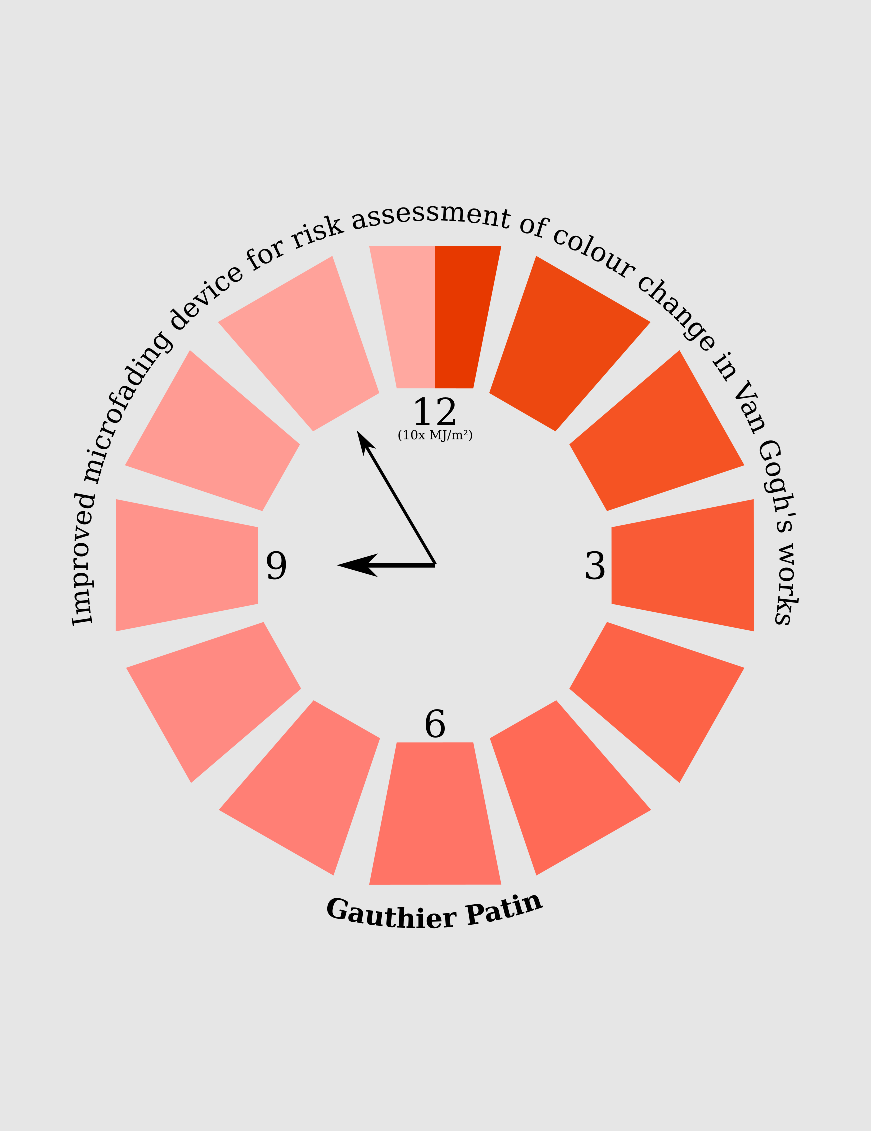
\includepdf[pages=1]{Covers/cover-front.pdf}

%% Title pages

% !TEX root = main.tex

\newgeometry{top=2.170cm,
            bottom=3.510cm,
            inner=2.1835cm,
            outer=2.1835cm,
            ignoremp}

%% Title page

\begin{titlepage}
   \begin{center}
       \vspace*{4cm}

       \textbf{\Huge Improved microfading device for risk assessment of colour change in Van Gogh's works}
           
       \vspace{7cm}
       
       \textbf{\Large Gauthier Patin}          
              
   \end{center}
\end{titlepage}


%% Copyright page

\null%
\label{thesis:colophon}
\vfill
\pdfbookmark[1]{Colophon}{thesis:colophon}

Written in 2018--2023 by Gauthier Patin 

ISBN: 978909037535

Copyright \copyright \hspace{0.1cm}2023 by Gauthier Patin

Printed by Proefschriftmaken, \url{https://www.proefschriftmaken.nl}\\

\vspace{0.5cm}

\textbf{Colophon} \\

This thesis was typeset with the help of \LaTeX{} and to a large extent uses the source code provided by Ken Arroyo Ohori for his PhD thesis (\url{https://github.com/kenohori/thesis}). Most of the figures were created using Inkscape or the Matplotlib and Searborn packages inside Jupyter notebooks.

The source code of this thesis is available at: \url{https://github.com/g-patin/PhD_thesis}

A digital version of this dissertation is available on the Digital Academic Repository of the University of Amsterdam (\url{https://dare.uva.nl}) as well on my PhD website (\url{https://microfadingphd.wordpress.com}). 

The data that have been used to create the figures in Chapters 3, 4, and 5 have been stored on a Zenodo repository (\url{https://zenodo.org/record/8216110}). \\

\vspace{0.5cm}

\textbf{Cover} \\

The front and back covers are based on the results of light ageing experiments conducted during this PhD using the methodology described in Chapter 4 (section \ref{sec:DL_methodology}) of this dissertation. Both covers display the results of daylight exposure on an eosin paint-out (PO098). The front cover shows visualization of colour patches as the light dose increases from 0 to 120 MJ/m\textsuperscript{2}, while the back cover shows differences in the reflectance spectra as the light dose increases from 0 to 120 MJ/m\textsuperscript{2}. A value of 120 MJ/m\textsuperscript{2} roughly corresponds to 50 years of continuous exposure in the galleries of the Van Gogh Museum (10 hours per day at 50 lux).



%% A two-page pdf provided to me by the UvA once my dissertation had been accepted.


\includepdf[pages=1]{P30_ATTACH_corrected.pdf}

\includepdf[pages=2]{P30_ATTACH_corrected.pdf}


%% Funding statement

\newpage
{\Large\textbf{Funding}}\\

The research for this thesis received financial assitance from the AXA Research Fund, the Van Gogh Museum-ASML Partnership in Science, the Rijksdienst voor het Cultureel Erfgoed, and the Rijksmuseum Amsterdam. 

\vspace{1.5cm}

\begin{figure}[!h]
\centering

\includegraphics[width=0.75\textwidth]{Logo_institutions.png}
\label{fig:colours_description}
\end{figure}

\newpage
\newpage


%% TOC - Figures - Tables - Equations - Acronyms
\newpage
\tableofcontents
\newpage
\listoffigures
\newpage
\listoftables

\listofmyequations

\printglossary[style=long, title=Acronyms]

% !TEX root = main.tex

\addchap{Abstract}

Over the past three decades, conservators and curators at the Van Gogh Museum have gathered increasing evidence of colour changes having occurred in Van Gogh’s paintings. Numerous research projects on colour change in Van Gogh’s works, conducted since the 1990s, have greatly deepened our knowledge on the issue and are reviewed in Chapter \ref{ch:ch1_general-intro}. For instance, the light-sensitive pigments responsible for these colour changes have been identified and their degradation mechanisms investigated. Additionally, light-ageing experiments on paint-outs were conducted and several attempts to estimate the original appearance of paintings carried out. Yet, our actual knowledge of the timescale of this problem is rather limited. To what extent has the observed fading and discolouration in Van Gogh’s paintings now stabilised? And if still ongoing, how fast does it occur? In other words, can we expect to see colour changes taking place in Van Gogh’s paintings over the next ten years or so? The work performed during the timeframe of this PhD contributes towards providing answers to these questions, by supplying reliable data for light fading risk assessment on which to base decisions regarding the long-term preservation of the paintings. \\

In the late 1990s, researchers in the \gls{USA} and \gls{UK} developed devices to monitor light-induced colour change at a microscale level. This technique, known as microfadeometry and thoroughly described in Chapter \ref{ch:ch2_MFT}, enables lightfastness analyses on objects, helping museum professionals to make decisions regarding the illumination of their collections. Nevertheless, the technique presents a number of limitations, which hinders reliable interpretation of the data. The specific aim of this PhD project is to improve microfading analyses on technical and methodological levels so that it can take us closer towards reliable colour change prediction. \\ 

In this respect, the PhD project focused on three topics related to microfadeometry. The first one aimed to make technical progress regarding the way microfading analyses are being performed (Chapter \ref{ch:ch3_MFT-advances}, section \ref{sec:stereo-MFT}). The second was intended to improve our knowledge on the rise of temperature at the surface of materials irradiated by a microfading beam (Chapter \ref{ch:ch3_MFT-advances}, section \ref{sec:MFT-Temp}). The third topic aimed to evaluate the accuracy of microfading data by assessing the validity of the reciprocity principle on several appropriate paint samples (Chapter \ref{ch:ch3_MFT-advances}, section \ref{sec:MFT-reciprocity}) and by comparing microfading data with traditional light-ageing methods (Chapter \ref{ch:ch4_light-ageing}). \\

The technical improvements accomplished led to the development of a new system called the stereo-MFT, which is presented in Chapter \ref{ch:ch3_MFT-advances}, section \ref{sec:stereo-MFT}. This new device uses a stereomicroscope as its central element for which the optics – in combination with a high-quality microscope camera – enables a better characterisation of the microfading beam. Ultimately, it improves the accuracy of our estimation of the amount of energy received by the sample, suggesting that dose-response microfading analyses can be performed with precision. Applications of the device on paint and textiles samples furthermore enabled us to outline several of its limitations that could potentially be resolved during future research projects to bring further improvements (Chapter \ref{ch:ch5_applications-MFT}). \\

The use of an infrared temperature sensor successfully provided surface temperature measurements of paint samples irradiated by a microfading beam (Chapter \ref{ch:ch3_MFT-advances}, section \ref{sec:MFT-Temp}). The results showed an increase of temperature significantly higher than most values reported in the literature. An increase of temperature ranging from 9\unit{\degreeCelsius} to 49\unit{\degreeCelsius} has been observed for the colours most frequently analysed with microfadeometry: yellow, oranges and reds. Additionally, the implementation of a mathematical model to simulate temperature changes and heat transfer inside irradiated materials proved to be a valuable tool to understand the influence of certain parameters on the heat transfer behaviour inside paint layers. For instance, parameters related to the light beam (power, size) or to the materials (thermal conductivity, specific heat capacity, heat transfer coefficient, density, etc.) can be studied. \\ 

The reliability of microfading data is directly related to the reciprocity principle. Research on this principle necessitates accurate characterization of the microfading beam in terms of spectral power distribution and light dose exposure, either in \unit{\lux\hour} or in \unit{\mega\joule\per\square\metre}. The reciprocity principle experiments (Chapter \ref{ch:ch3_MFT-advances}, section \ref{sec:MFT-reciprocity}) and the comparison with other light-ageing methods (Chapter \ref{ch:ch4_light-ageing}) confirmed failures of the principle and a lack of correlation with colour change occurring under normal conditions for half of the samples. Interpretation of the data enabled us to propose some technical and methodological ways to bypass this problem such as the use of colour change rate as a more appropriate metric for applying microfading data to works of art in the framework of lighting policies. \\

In a global way, all results obtained in this thesis converge on a single conclusion: microfadeometry is an effective and efficient technique for the detection and analysis of colour change phenomena. At the same time, it has not yet revealed its full potential, which, in my opinion, lies in its ability to correlate its point-wise results with other analytical data. Given the increasing importance of imaging techniques in cultural heritage science over the past decades, it seems relevant to orient microfading analyses in this direction with the intention of creating a computer-controlled motion system whereby microfading spots could be assigned $x$ and $y$ coordinates to precisely locate them on objects. While allowing a connection of microfading results with other data, this could also lead to image-based colour change prediction.

\addchap{Samenvattig}


In talrijke onderzoeksprojecten hebben restauratoren en conservatoren van het Van Gogh Museum in de afgelopen drie decennia steeds meer bewijs gevonden voor kleurveranderingen in de schilderijen van Van Gogh. Deze bevindingen hebben onze kennis over dit onderwerp aanzienlijk verdiept. De lichtgevoelige pigmenten die verantwoordelijk zijn voor deze kleurveranderingen zijn bijvoorbeeld geïdentificeerd en hun afbraakmechanismen zijn onderzocht. Daarnaast zijn lichtverouderingsexperimenten op verfmonsters uitgevoerd en verschillende pogingen om het oorspronkelijke uiterlijk van schilderijen te schatten. Toch is onze feitelijke kennis van de tijdschaal van dit probleem vrij beperkt. In hoeverre is de waargenomen verbleking en verkleuring van Van Gogh's schilderijen nu gestabiliseerd? En als het nog steeds doorgaat, hoe snel gaat het dan? Kunnen we bijvoorbeeld verwachten dat de kleurveranderingen op Van Gogh's schilderijen de komende ongeveer tien jaar zullen plaatsvinden? Deze aspecten worden in hoofdstuk \ref{ch:ch1_general-intro} besproken. Het werk dat in het kader van dit proefschrift is uitgevoerd, draagt bij aan de beantwoording van deze vragen door betrouwbare gegevens te leveren voor de beoordeling van het risico op verbleking en andere kleurveranderingen, op basis waarvan beslissingen kunnen worden genomen over de conservering van de schilderijen op de lange termijn.



Eind jaren 1990 ontwikkelden onderzoekers in de VS en het VK instrumenten om door licht veroorzaakte kleurverandering op microscopisch niveau te monitoren. Deze techniek, bekend als ‘microfadeometry’ en uitvoerig beschreven in hoofdstuk \ref{ch:ch2_MFT}, maakt analyses van de lichtechtheid van objecten mogelijk (vanaf hier genoemd microfadeometry of microfading analyses) en helpt ‘museum professionals’ om beslissingen te nemen over een optimale belichting van hun collecties. De techniek heeft echter een aantal beperkingen die een betrouwbare interpretatie van de gegevens in de weg staan. Het specifieke doel van dit PhD-project is om microfading analyses op technisch en methodologisch niveau te verbeteren, zodat het ons dichter bij een betrouwbare voorspelling van kleurveranderingen kan brengen. 

Hiervoor richtte het PhD-project zich op drie onderwerpen met betrekking tot microfadeometry. De eerste was gericht op het boeken van technische vooruitgang met betrekking tot de manier waarop microfading analyses worden uitgevoerd (Hoofdstuk \ref{ch:ch3_MFT-advances}, sectie \ref{sec:stereo-MFT}). Het tweede was gericht op het verbeteren van onze kennis over de temperatuurstijging aan het oppervlak van materialen die bestraald worden door een microfading lichtbundel (Hoofdstuk \ref{ch:ch3_MFT-advances}, sectie \ref{sec:MFT-Temp}). Het derde onderwerp was bedoeld om de nauwkeurigheid van microfading data te evalueren door de geldigheid van het reciprociteitsprincipe te beoordelen op verschillende geschikte verfmonsters (hoofdstuk \ref{ch:ch3_MFT-advances}, sectie \ref{sec:MFT-reciprocity} en door microfading data te vergelijken met traditionele lichtverouderingsmethoden (hoofdstuk \ref{ch:ch4_light-ageing}).


De bereikte technische verbeteringen leidden tot de ontwikkeling van een nieuw systeem genaamd de stereo-MFT, dat wordt gepresenteerd in hoofdstuk \ref{ch:ch3_MFT-advances}, sectie \ref{sec:stereo-MFT}. Dit nieuwe instrument maakt gebruik van een stereomicroscoop als centraal element waarvan de optiek - in combinatie met een hoogwaardige microscoopcamera - een betere karakterisering van de microfading lichtbundel mogelijk maakt. Uiteindelijk verbetert het de nauwkeurigheid van onze schatting van de hoeveelheid energie die het oppervlak van object ontvangt, wat suggereert dat dosis-respons microfading analyses met precisie kunnen worden uitgevoerd. Toepassingen van het apparaat op verf- en textielmonsters vermijden ons bovendien in staat om een aantal beperkingen aan te geven die mogelijk opgelost kunnen worden tijdens toekomstige onderzoeksprojecten (Hoofdstuk \ref{ch:ch5_applications-MFT}).

Het gebruik van een infrarood temperatuursensor leverde met succes metingen op van de oppervlaktetemperatuur van verfmonsters die bestraald werden door een microfading lichtbundel (hoofdstuk \ref{ch:ch3_MFT-advances}, sectie \ref{sec:MFT-Temp}). De resultaten toonden een temperatuurstijging die aanzienlijk hoger was dan de meeste waarden die in de literatuur werden gerapporteerd. Een temperatuurstijging van 9 tot 49 graden Celsius werd waargenomen voor de kleuren die het meest werden geanalyseerd met microfadeometrie: geel, oranje en rood. Daarnaast bleek de implementatie van een wiskundig model om temperatuurveranderingen en warmteoverdracht binnen bestraalde materialen te simuleren een waardevol hulpmiddel om de invloed van bepaalde parameters op het warmteoverdrachtsgedrag binnen verflagen te begrijpen. Zo kunnen bijvoorbeeld parameters met betrekking tot de lichtbundel (vermogen, grootte) of de materialen (warmtegeleidingsvermogen, specifieke warmtecapaciteit, warmteoverdrachtscoëfficiënt, dichtheid, enz.) worden bestudeerd. 

De betrouwbaarheid van gegevens over microfading houdt rechtstreeks verband met het reciprociteitsprincipe. Onderzoek naar dit principe vereist een nauwkeurige karakterisering van de microfadingsbundel in termen van spectrale vermogensverdeling en blootstelling aan lichtdosis, hetzij in \unit{\lux\hour} of in \unit{\mega\joule\per\square\metre}. De experimenten met het reciprociteitsprincipe (hoofdstuk \ref{ch:ch3_MFT-advances}, sectie \ref{sec:MFT-reciprocity}) en de vergelijking met andere lichtverouderingsmethoden (hoofdstuk \ref{ch:ch4_light-ageing}) bevestigden voor de helft van de monsters de tekortkomingen van het principe en een gebrek aan correlatie met kleurverandering onder normale omstandigheden. Door de gegevens te interpreteren konden enkele technische en methodologische manieren worden voorgesteld om dit probleem te omzeilen, zoals het gebruik van kleurveranderingssnelheid als een meer geschikte metriek voor het toepassen van microfading data op kunstwerken in het kader van verlichtingsbeleid.

Globaal gezien komen alle resultaten die in dit proefschrift zijn verkregen tot één conclusie: microfadeometrie is een effectieve en efficiënte techniek voor de detectie en analyse van kleurveranderingsverschijnselen. Tegelijkertijd heeft het nog niet zijn volledige potentieel laten zien, dat naar mijn mening ligt in het vermogen om de puntsgewijze resultaten te correleren met andere analytische gegevens. Gezien het toenemende belang van beeldvormingstechnieken in de culturele erfgoedwetenschappen in de afgelopen decennia, lijkt het relevant om de microfading analyses in deze richting te oriënteren met de bedoeling om een computergestuurd bewegingssysteem te creëren waarbij aan de microfading plekken $x,y$ coördinaten kunnen worden toegekend om ze precies op objecten te lokaliseren en te documenteren. Terwijl het een verbinding mogelijk maakt van microfading resultaten met andere gegevens, zou dit ook kunnen leiden tot beeldgebaseerde voorspelling van kleurveranderingen.




\addchap{Résumé}

Au cours des trois dernières décennies, les restaurateurs et les conservateurs du musée Van Gogh ont recueilli de plus en plus d'indices de changements de couleur dans les peintures de Van Gogh. De nombreux projets de recherche sur les changements de couleur dans les œuvres de Van Gogh, menés depuis les années 1990, ont considérablement approfondi nos connaissances sur la question et sont passés en revue au sein du chapitre \ref{ch:ch1_general-intro}. Ainsi, les pigments sensibles à la lumière responsables de ces changements de couleur ont été identifiés et leurs mécanismes de dégradation étudiés. En outre, des expériences de vieillissement à la lumière ont été menées sur des reconstructions et plusieurs tentatives d'estimation de l'aspect original des peintures ont été réalisées. Cependant, nos connaissances actuelles sur l'échelle de temps de ce problème sont plutôt limitées. Dans quelle mesure la décoloration observée dans les peintures de Van Gogh s'est-elle stabilisée ? Et si elles se poursuivent, à quelle vitesse se produisent-elles ? En d'autres termes, peut-on s'attendre à ce que les peintures de Van Gogh subissent des changements de couleur au cours des dix prochaines années environ ? Les travaux réalisés dans le cadre de cette thèse contribuent à apporter des réponses à ces questions, en fournissant des données fiables pour l'évaluation des risques d'altération par la lumière, sur lesquelles fonder les décisions relatives à la conservation à long terme des peintures. \\

À la fin des années 1990, des chercheurs américains et britanniques ont mis au point des dispositifs permettant d'évaluer les changements de couleur induits par la lumière à l'échelle microscopique. Cette technique, connue sous le nom de \textit{micro-décoloration} ou "microfadéométrie" (\textit{microfading test} ou \textit{microfadeometry} en anglais) et décrite en détail au chapitre \ref{ch:ch2_MFT}, permet d'analyser la résistance à la lumière des objets, aidant ainsi les professionnels des musées à prendre des décisions concernant l'éclairage de leurs collections. Néanmoins, la technique présente un certain nombre de limitations qui empêchent une interprétation fiable des données. L'objectif spécifique de ce projet de doctorat est d'améliorer les analyses de micro-décoloration sur les plans technique et méthodologique afin de nous rapprocher d'une prédiction plus fiable des changements de couleur. \\

À cet égard, le projet de doctorat s'est concentré sur trois sujets liés à la micro-décoloration. Le premier visait à réaliser des progrès techniques concernant la manière dont les analyses de micro-décoloration sont effectuées (chapitre 1, section \ref{sec:stereo-MFT}). Le second avait pour but d'améliorer nos connaissances sur l'augmentation de la température à la surface des matériaux irradiés par un faisceau lumineux intense (chapitre 3, section \ref{sec:MFT-Temp}). Le troisième sujet visait à évaluer la précision des données de micro-décoloration en évaluant la validité du principe de réciprocité sur plusieurs échantillons de peinture (chapitre 3, section \ref{sec:MFT-reciprocity}) et en comparant les données de micro-décoloration avec les méthodes traditionnelles de vieillissement à la lumière (chapitre 4). \\

Les améliorations techniques réalisées ont conduit au développement d'un nouveau système appelé stéréo-MFT, qui est présenté au chapitre \ref{ch:ch3_MFT-advances}, section \ref{sec:stereo-MFT}. Ce nouveau dispositif utilise un stéréomicroscope comme élément central pour lequel le système d'optique - en combinaison avec une caméra de microscope de haute qualité - permet une meilleure caractérisation du faisceau lumineux. En fin de compte, cela améliore la précision de notre estimation de la quantité d'énergie reçue par l'échantillon, suggérant que les analyses de micro-décoloration en fonction de la dose énergétique peuvent être effectuées avec précision. L'application de l'appareil sur des échantillons de peinture et de textile nous ont en outre permis de mettre en évidence plusieurs de ses limites, qui pourraient être résolues dans le cadre de futurs projets de recherche afin d'apporter de nouvelles améliorations (chapitre \ref{ch:ch5_applications-MFT}). \\

L'utilisation d'un capteur de température infrarouge a permis de mesurer la température de surface d'échantillons de peinture irradiés par un faisceau de micro-décoloration (chapitre \ref{ch:ch3_MFT-advances}, section \ref{sec:MFT-Temp}). Les résultats ont montré une augmentation de la température significativement plus élevée que la plupart des valeurs rapportées dans la littérature. Une augmentation de la température allant de 9\unit{\degreeCelsius} à 49\unit{\degreeCelsius} a été observée pour les couleurs les plus fréquemment analysées par microfadéométrie : le jaune, l'orange et le rouge. En outre, la mise en oeuvre d'un modèle mathématique pour simuler les changements de température et le transfert de chaleur à l'intérieur des matériaux irradiés s'est avérée être un outil précieux pour comprendre l'influence de certains paramètres sur le comportement du transfert de chaleur à l'intérieur des couches de peinture. Par exemple, les paramètres liés au faisceau lumineux (puissance, taille) ou aux matériaux (conductivité thermique, capacité thermique spécifique, coefficient de transfert de chaleur, densité, etc) peuvent être ainsi étudiés.\\


La fiabilité des données de micro-décoloration est directement liée au principe de réciprocité. La recherche sur ce principe nécessite une caractérisation précise du faisceau lumineux en termes de distribution de puissance énergétique et d'exposition à la dose de lumière, soit en lx.hr, soit en MJ/m\textsuperscript{2}. Les expériences sur le principe de réciprocité (chapitre \ref{ch:ch3_MFT-advances}, section \ref{sec:MFT-reciprocity}) et la comparaison avec d'autres méthodes de vieillissement par la lumière (chapitre \ref{ch:ch4_light-ageing}) ont confirmé les échecs du principe et l'absence de corrélation avec le changement de couleur survenant dans des conditions normales pour la moitié des échantillons. L'interprétation des données nous a permis de proposer des moyens techniques et méthodologiques pour contourner ce problème, comme l'utilisation du taux de changement de couleur en tant que mesure plus appropriée pour appliquer les données de micro-décoloration aux oeuvres d'art dans le cadre des politiques d'éclairage.\\

D'une manière générale, tous les résultats obtenus dans cette thèse convergent vers une seule conclusion : la micro-décoloration est une technique efficace pour la détection et l'analyse des phénomènes de changement de couleur. En même temps, elle n'a pas encore révélé tout son potentiel, qui, à mon avis, réside dans sa capacité à corréler ses résultats avec d'autres données analytiques. Étant donné l'importance croissante des techniques d'imagerie dans la science du patrimoine culturel au cours des dernières décennies, il semble pertinent d'orienter les analyses de micro-décoloration dans cette direction avec l'intention de créer un système contrôlé par ordinateur dans lequel chaque analyse de micro-décoloration pourrait être assignées à des coordonnées $x$ et $y$ afin de les localiser précisément sur les objets. Tout en permettant de relier les résultats de la décoloration à d'autres données, ce système pourrait également permettre de prédire les changements de couleur à l'échelle de l'une oeuvre dans sa globalité.
\afterpage{\blankpage}


%\newgeometry{top=2.170cm,
%            inner=2.1835cm,
%            outer=2.1835cm,
%            bottom=3.510cm,
%            ignoremp}
\restoregeometry


%% Chapters

\newpage
% !TEX root = main.tex

\newcommand{\HRule}{\rule{\linewidth}{0.5mm}} 	% horizontal line and its thickness

%%%% Title Page

\newgeometry{top=2.170cm,
            bottom=3.510cm,
            inner=2.1835cm,
            outer=2.1835cm,
            ignoremp}

\pagecolor{mygray}

\begin{titlepage}
   \begin{center}
       \vspace*{3cm}
       {\fontsize{40pt}{46pt}\selectfont \textbf{Chapter 1}}\\       
       \vspace*{3cm}
       {\fontsize{30pt}{36pt}\selectfont \textbf{General} \\[1cm] 
        \fontsize{30pt}{36pt}\selectfont \textbf{introduction}} \\           
   \end{center}
\end{titlepage}


\pagecolor{white}
\restoregeometry


\chapter{ General introduction}
\label{ch:ch1_general-intro}

This general introduction is divided into four main sections. It starts with a short explanation of light-induced colour change on cultural heritage objects as the central topic of this dissertation, going on to describe the latter in the next section. A third section on the challenge of light management in cultural heritage institutions gives the reader the ground knowledge necessary to connect the outcomes of this project to the practice of conservation in institutions. Finally, in order to place this research in a historical context, the last section provides an overview of past studies on colour changes in Van Gogh's works. \\



%%%%%%% The phenomenon of light-induced colour change on cultural heritage objects %%%%%%%

\section{The phenomenon of light-induced colour change on cultural heritage objects}


From a materials perspective, a colour change consists of a shift in colour perception of a surface over time. Although scientific tools and methods have been developed to mathematically express colours and colour changes in a precise and objective way, it is important to remember that colour and colour change are perceptual phenomena. This means that the appearance and interpretation of a colour or a colour shift also depends on the response of the observer from a physiological, psychological and cultural point of view. In other words, we can quantify a colour change in an objective way, but whether or not we find it to be disturbing or even consider it as damage  cannot be determined with exact science tools, as Salvador Mu\~noz Vi\~nas noted: 

\textit{It is very interesting to note that neither intention nor value are material, scientifically determinable factors, so that ultimately the all-important notion of damage is neither within the reach of science, nor is it a property of the object, but the result of a personal subjective judgement.} \citep[102]{munoz_vinas_contemporary_2005}. \\


\marginpar{
\captionsetup{type=figure}
\includegraphics[width=4cm]{Chapters/Chapter1_General_Introduction/Figures/Materials_values_1.png}
\caption[\hspace{0.3cm}Values-materials relationship]{Values-materials relationship.}
\label{fig:values_materials}
}


Cultural heritage objects are no more than the sum of various materials assembled together to which society attributes some specific values, making a difference between the bicycle wheel in your garage and the one displayed at the Centre Pompidou in Paris – although both wheels might be virtually identical from a material point of view. The interdependency between values and materials is a key aspect of cultural heritage artefacts (Figure \ref{fig:values_materials}). As a visitor, the interaction with these objects is initially visual in most cases, allowing access to the values of the objects. In conservation, we begin by establishing the values of the objects, so that our actions on the materials can influence the values appropriately. In other words, the materials of cultural heritage objects form both a carrier and a gateway to the values and information they convey. Environmental agents can directly affect materials and modify their aesthetics, which ultimately can cause a change in the values and meanings conveyed to the observer. For example, the ink on a letter can vanish hampering our ability to read its content, or the highlights on a painting may become less visible thereby modifying the effect of tonal contrast.\\


Among the many factors causing colour change on materials, exposure to optical radiation is responsible for the majority of colour change occurring on objects\sidenote{Exposure to optical radiation may also weaken the physical structure of objects through cracking and embrittlement \citep[p.126]{saunders_museum_2020}.}. Unlike other environmental agents – such as temperature, relative humidity and, oxygen concentration – light is the only one that cannot be removed without preventing visual access to the object. Any use of the object by a person requires it to be illuminated, which can potentially result in colour changes. \\


\begin{figure}[!h]
\centering
\includegraphics[width=0.8\textwidth]{Chapters/Chapter1_General_Introduction/Figures/colour_description_1.png}
\caption[\hspace{0.3cm}Description of colours]{Description of colours.}
\label{fig:colours_description}
\end{figure}


There are three main ways of describing colours and colour changes: verbally, visually and numerically (Figure \ref{fig:colours_description}). Although an abundant vocabulary gives us the possibility to convey a fair estimation of colour, in the context of a scientific research project, words lack precision and objectivity\sidenote{Limitations of language in the field of conservation have also been outlined by \citet{bucklow_description_1997} when studying craquelure patterns on paintings.}. This is why, in the framework of this PhD project, visual and numerical description of colours will mainly be used. From a colorimetric perspective, variations within a colour can be divided into three types of change, which are themselves derived from colourimetric characterisation of colours. A colour can vary in lightness ($L^*$  in the CIELAB colour space)\sidenote{More information about the \gls{CIE} colour spaces can be found in Chapter 2, section \ref{sec:colour_measurement}.}, becoming darker or lighter. It can also alter in saturation ($C^*$ metric); usually a colour becomes less saturated upon light exposure, thus appearing less intense or greyer. Finally, and more rarely seen, the hue of a colour can shift ($h$ metric). Such change is usually observed for thermochromic substances which undergo a reversible change of colour when heated or cooled. \\


Although the risk of colour change due to light exposure is higher than for any other risk factor causing colour change, it does not mean that the risks for museum objects today are higher than they were in the past. Over the last 25 years, the number of exhibited objects has not noticeably increased\sidenote{\url{https://www.egmus.eu/nc/en/statistics/complete_data/} (accessed 15/07/2021).} and the light intensity levels for exhibition have even tended to decrease. But our practices of conservation and our perception of colour change phenomena have evolved. Studies on colour changes conducted since the late 1990s have increased awareness among cultural heritage professionals\sidenote{A review of past studies in colour changes in Van Gogh is provided in section \ref{sec:overview_past_studies}} as well as the general audience\sidenote{Articles in mainstream newspapers help to bring the topic into the public space. An illustrative list of articles is given in Appendix \ref{app:ch1_articles_lid}}. In addition, the development of preventive conservation led to the need for more accurate predictive data in support of decision-making for collection care strategies. Moreover, lighting systems have evolved considerably over the last decades, with more frequent use made of \gls{LED} light sources in exhibition spaces. The dynamism of this latter technology forces the cultural heritage community to perform their own research in order to assess and validate the use of LEDs for the illumination of cultural objects \citep{michalski_led_2020}. All in all, the motivation to pursue this research topic in the form of a PhD was created by new \gls{LED} lighting installations in the exhibition spaces of the Van Gogh Museum\sidenote{In 2015–2016, the Van Gogh Museum replaced halogen light sources with \gls{LED} lamps: Domenico Casillo, light designer at the Van Gogh Museum, personal communication, 10/10/2018). } and increased awareness of the impact of light-induced colour change based on the research performed over the last decades on the Van Gogh Museum collections.\\



%%%%%%% About this thesis %%%%%%%

\newpage
\section{About this thesis}

\subsection{Subject}

\marginpar{
\captionsetup{type=figure}
\includegraphics[width=\marginparwidth]{Chapters/Chapter1_General_Introduction/Figures/PhD_intersection_fields.png}
\caption[\hspace{0.3cm}Fields of knowledge within the PhD project]{Fields of knowledge within the PhD.}
\label{fig:knowledge_fields}
}

The subject of this PhD lies at the intersection of three distinct fields of knowledge (Figure \ref{fig:knowledge_fields}). The first relates to the technical development of tools for studying the lightfastness of materials, specifically those used in works of art. Since the last decade of the 20\textsuperscript{th} century, our ability to assess the stability of coloured materials exposed to light has improved through the development of \gls{MFT} \citep{pretzel_determining_2000, whitmore_predicting_1999}. The second field concerns paint and colour technology, which is essential when attempting to understand the materiality of works of art. For example, 'historically accurate’\sidenote{There is an ongoing debate regarding use of the term 'historically accurate', other terms such as 'historically influenced, appropriate or informed' have been proposed instead \citep{carlyle_reconstructions_2020}.} paint reconstructions used in several research projects over the last two decades have proved to be an important element for interpreting phenomena observed on actual objects \citep{carlyle_historically_2007}. The last field of knowledge discussed in this thesis deals with the study of colour and colour changes in Van Gogh's paintings and works on paper. It is a known fact that some of the colours used by Van Gogh change upon light exposure and over the past three decades, conservators and curators have gathered increasing evidence of colour changes having occurred in Van Gogh’s paintings \citep{hendriks_paintings_2016} as well as in drawings (\citealp{meedendorp_hand--hand_2013,shelley_technical_2005}; \citealp[428]{vellekoop_van_2013}). While past studies on colour changes in Van Gogh’s works have greatly deepened our knowledge on the issue, they also raised more questions and opened up new avenues for conservation practice that have yet to be explored. This doctoral research aims to take a next step by combining knowledge from the three aforementioned fields linked to the study of light-induced colour change and focusing on the development and application of an improved microfading methodology to study colour changes in Van Gogh's works. \\

\subsection{Research questions and objectives}



Although, the light-sensitive pigments responsible for the colour changes occurring on Van Gogh's works have been identified and their degradation mechanisms investigated \citep{bommel_investigation_2005, burnstock_comparison_2005, monico_degradation_2013-1}, our actual knowledge of the timescale of this problem is rather limited. For example, to what extent has the observed fading and discolouration in Van Gogh’s paintings now stabilised? And if still ongoing, how fast does it occur – can we expect to see colour changes taking place in Van Gogh's artworks over the next ten or twenty years? Although answering these questions lies beyond the scope of this thesis, they were crucial for determining the direction of this work. To provide answers requires valid data on which to base decisions regarding the long-term preservation of the paintings. Supplying the museums with reliable data for light-fading risk assessment is the ultimate goal of this research (Figure \ref{fig:PhD_objectives}, yellow circle). Centred around this main objective, the project is structured in three main parts, each with its own goals (Figures \ref{fig:PhD_objectives} and \ref{fig:PhD_work_packages}, green rectangles). The first part aims to improve microfadeometry by implementing a new device along with its methodology. The purpose of the second part is to increase our knowledge and understanding of 19\textsuperscript{th} century paint materials as well as colour change phenomena. Once these two objectives have been met, a third part of the project will entail the application of microfadeometry to a variety of samples for which the light exposure risk can be modelled. \\

\begin{figure*} %[!h]
\centering
\includegraphics[width=\linewidth]{Chapters/Chapter1_General_Introduction/Figures/PhD_objectives.png}
\caption[\hspace{0.3cm}Objectives of the PhD]{Objectives of the PhD.}
\label{fig:PhD_objectives}
\end{figure*}

The three main parts of the project also aim for some longer-term goals (Figure \ref{fig:PhD_objectives}, blue rectangles). Firstly, through the communication of research outcomes as well as collaborative projects with other institutions, I hope that the improvements accomplished within the field of microfadeometry will carry forward into the conservation, scientific and industrial communities. For example, some of the technical improvements may be implemented by industrial partners for the next generation of microfading devices. Similarly, the knowledge acquired on colour changes observed in 19\textsuperscript{th} century paint materials in the second part of the project can be used for improved digital visualisations of artworks providing useful tools to solicit viewers’ opinion on perceived changes. Lastly, the provision of reliable microfading data will benefit the long-term conservation of artworks when utilised within the framework of a lighting policy.


\subsection{Structure and methodology}

In accordance with the previously described fields of knowledge and PhD objectives, the PhD work programme is structured in three main parts (Figure \ref{fig:PhD_work_packages}, green rectangles). Several interdependent sub-research projects (light blue rectangles) bind together the three main strands of research. For example, projects 1.3, 2.2, 2.3 and 3.1 all use model paint-outs that have been created in project 2.1. Chapter 3 of this thesis draws together all the projects from Part 1, while Chapter 4 compares the results of different light-ageing techniques therefore including sub-projects from parts 2 and 3, specifically 2.2, 2.3 and 3.1. The application of microfadeometry to museum objects is discussed briefly in Chapter 5. \\

The following subsections aim to introduce the types of sample and analytical methods employed for this PhD project. More detailed information about sample preparation and analytical parameters is given within the section of each research project.\\

\begin{figure} %[!h]
\centering
\includegraphics[width=0.9\linewidth]{Chapters/Chapter1_General_Introduction/Figures/PhD_working_structure.png}
\caption[\hspace{0.3cm}Structure of the PhD thesis]{Structure of the PhD.}
\label{fig:PhD_work_packages}
\end{figure}

\subsubsection{Objects of investigation}

A variety of objects has been used throughout this PhD. This section gives a clear terminology for each of them.

\begin{itemize}
    \item \textbf{Reference samples}: Samples used internationally as references in the field of colourimetry and microfadeometry. These are typically Pantone, Macbeth ColorChecker, or BS381C \citep{british_standards_institution_bs_1996} colour charts and \gls{BWS} (DIN EN ISO 105-B02, \citep{deutsches_institut_fur_normung_ev_din_2001}). 	
    \item \textbf{Model \gls{PO}/reconstructions}: Contemporary paint layers reconstructed according to the physical and chemical properties of Van Gogh paintings. They are not paint layers from actual Van Gogh paintings but historically informed reproductions.
    \item \textbf{Cross-section samples}: Paint samples, taken from model paint-outs or from an original work of art, embedded in polyester resin and prepared as cross-sections.
\end{itemize}
 
\subsubsection{Analytical methods}

Throughout this PhD project, visible reflectance spectroscopy was the main technique of investigation employed. It was used either with the help of a photospectrometer, such as the CM-2600d from Konica Minolta, or as a self-assembled system in which a spectrometer was combined with a light source. The latter option was implemented in the microfading device developed in this project (Chapter 3, section \ref{sec:stereo-MFT}). Other devices were also used, mainly to monitor the environmental conditions such as the light energy (in photometric and radiometric units), temperature or relative humidity and are mentioned in detail within their corresponding sections.\\


\subsubsection{Data processing methods}


The processing of every data acquired during this PhD followed three main and general rules:

\begin{itemize}
\item \textbf{The use of simple and open-source file format.} The durability of the scientist's work often depends on ensuring long-term access to the research results. Consequently, as elaborated in Chapter \ref{ch:ch3_MFT-advances}, page \hyperlink{page.136}{136}, it was chosen to use open file format for this study, seen as the best way to ensure that files can continue to be opened in the future.  

\item \textbf{The use of programming languages.} The data generated by the analysis of samples and works of art is becoming increasingly important in terms of quantity and size. In other words, the number of analyses increases as well as the amount of information for each measurement. Additionally, new techniques and devices are regularly developed adding to the increasing amount of data. Faced with this mass of data, I believe that it is relevant to use IT tools that enable the data to be processed quickly and efficiently. Although traditional and popular data processing and visualisation software, such as the Microsoft Office programs, offer certain significant advantages, it is clear that they are not suited to repeated, automatic processing of data. Hence the need to use programming languages to process and visualise data. There is a large number of computer languages, each with their own advantages and disadvantages depending on the context of use. The Python language seems well suited to the cultural heritage field and compared to other languages is fairly easy to learn and thus accessible to most scientists. It also offers a wide range of tools for data processing and visualisation which is particularly relevant when combining imaging and point-wise data.

\item \textbf{The use of a unique digital platform.} Most of the time, various observational and analytical techniques are used to study or characterise the materials used in works of art. Visualising the results and data acquired with each tool often requires the use of specific software developed by the company that manufactured or sold the device. In other words, there are as many digital platforms as there are analysis devices, which makes it difficult to relate the results of different types of analysis. In the framework of this PhD project, a unique digital platform has been used to process and visualise the data acquired from various devices. This digital environment, called \textit{Jupyter}\sidenote{See the Jupyter website for more information: \url{https://jupyter.org/}}, enables the use of programming languages such as Python and offers the possibility to open  various types of files and formats (images, text, numerical data, pdf, etc.), which makes the Jupyter ecosystem very versatile and flexible. 
\end{itemize}




%%%%%%% Challenges of light management in cultural heritage institutions %%%%%%%

\newpage
\section{Challenges of light management in cultural heritage institutions}

\vspace{0.3cm}

\begin{figure*}[!h]
\centering
\includegraphics[width=0.88\textwidth]{Chapters/Chapter1_General_Introduction/Figures/Risk_management_2.png}
\caption[\hspace{0.3cm}Risk management context applied to lighting policy]{Risk management context applied to lighting policy.}
\label{fig:risk_management}
\end{figure*}

\vspace{0.3cm}

This section looks at colour change as seen from a conservation perspective within the framework of cultural institutions. The purpose is to study how museums respond to the phenomenon of colour change. In other words, how do cultural institutions deal with this issue and what kinds of methodology and tools can they utilise to face up to this challenge? \\ 

More broadly, the issue can be approached from a risk management perspective for which standard protocols \citep{international_organization_for_standardization_isotc_262_iso_2018} and procedures have been developed, such as the ABC method \citep{michalski_abc_2016} and QuiskScan \citep{brokerhof_quiskscanquick_2016}\sidenote{For a good introduction to the topic of risk management applied to cultural heritage objects see \citet[9-16]{brokerhof_risk_2017}.}. Addressing light-induced colour change from a risk management perspective can be akin to implementing a lighting policy framework which contains the risk management steps\sidenote{Section \ref{sec:lighting policy framework} focuses on the risk management steps.}. These steps can be applied from either a category-based or an object-based perspective (Figure \ref{fig:risk_management}). Although both approaches follow risk management procedures, the two methods of application differ.  \\ 

In the category-based approach, the lighting policy is defined as a set of written recommendations or rules guiding the illumination of cultural objects, hence the common use of the term illumination guidelines\sidenote{It is interesting to note that most guidelines focus on illumination levels in an exhibition context, ignoring exposure during conservation treatments. To my knowledge, Garry Thomson’s The Museum Environment is one of the rare publications to discuss it \citep[44]{thomson_museum_1978}.}. Many institutions have produced such documents in which the main information is displayed in a table classifying materials according to their light sensitivity, with guideline light exposure levels and duration given for each category (\citealp[Tables 1 and 2]{ashley-smith_continuing_2002}; \citealp[10–11, Tables 2 and 3]{instituut_collectie_nederland_het_2005})\sidenote{For a good review of existing guidelines up to 2010 see \citet[28-35]{del_hoyo-melendez_study_2010}. While minor developments have occurred since 2010, nothing has changed radically since that date so the information and comments provided by Julio del Hoyo-Meléndez are still valid.}. Although the number of light-sensitivity categories and recommended illuminance values might slightly differ from one institution to the next, most classify the objects in three categories of light sensitivity – high, moderate, low – with, respectively, their corresponding recommended illuminance range values – 50, 75–150, 200 lux or above; which is quite similar to the categories defined by \citet[23]{thomson_museum_1978}. The lighting decision for each object is defined by the category assigned to it. In other words, the approach starts from a generic group and then transfers the properties relating to that group to individual objects. The method is relatively easy and fast to implement since it does not require analyses or measurements on the objects. \\ 



Conversely, the object-based approach starts with analysis of the object, providing data that can be used to make decisions leading to specific actions for each object. When several objects have similar characteristics, the original data can be extrapolated to a collection of objects. Contrary to the previous approach, this one goes from a single object to a group of similar items. However, since it requires more time, money, and knowledge than the first approach, only larger institutions have access to such resources. \\

The following subsections explore the structure of the lighting policy framework in detail. The first starts with a description of the general context, defining the actors in play and their relationships. A second subsection poses the problem of the light dilemma which is directly related to colour change phenomena. And lastly, in a third subsection, the methodology and tools available to cultural institutions in order to confront this matter are reviewed. Since very comprehensive and up-to-date publications on the aspect of light management by cultural heritage institutions are available, such as \citet{michalski_light_2018} and \citet{saunders_museum_2020}, I will refer to the state-of-the-art knowledge they present rather than repeating this information in this dissertation.\\

\subsection{Institutional context}

Although in 2022, the updated definition of a museum given by the \gls{ICOM} mentions several objectives\sidenote{“A museum is a not-for-profit, permanent institution in the service of society that researches, collects, conserves, interprets and exhibits tangible and intangible heritage. Open to the public, accessible and inclusive, museums foster diversity and sustainability. They operate and communicate ethically, professionally and with the participation of communities, offering varied experiences for education, enjoyment, reflection and knowledge sharing.” (ICOM definition adopted on August 24\textsuperscript{th} 2022)
(\url{https://icom.museum/en/resources/standards-guidelines/museum-definition/} , accessed on 05/01/2023).}, globally speaking, the objectives of cultural institutions can be summed up in just two words: preservation and dissemination. The primary mission of these institutions is the preservation of cultural heritage, first by collecting objects of interest and then by preserving their material integrity through conservation measures while enhancing their associated meanings and values through studies and research activities from a conservation, curatorial and scientific point of view. By dissemination, I mean all activities involving the collection and seeking for communication with external parties. It includes a broad range of activities such as sharing knowledge related to the objects and their makers, encouraging others to learn about the collection, inspiring people, supporting research projects on the collection, and is carried out through publications as well as through the organisation of periodic or permanent events, ranging from group workshops to temporary exhibitions on a specific subject.\\

Exhibiting objects, works of art or not, always involves four main actors\sidenote{The exhibition context can be approached through the \gls{ANT}, hence the use of the word actor to refer to both people and objects. More information about \gls{ANT} can be found on \url{https://en.wikipedia.org/wiki/Actor\%E2\%80\%93network_theory}, accessed on 06/01/2023.}: the item itself, a light source to be able to see the item, an observer that acknowledges the object's presence and a setting such as an institution that links the aforementioned actors in a single context (Figure \ref{fig:institution_exhibition} - a). Each actor within the exhibition ecosystem has a set of parameters (Figure \ref{fig:institution_exhibition} - b, italic text) that will need to be characterised by the institution. It is also important for the institution to fully and properly control the light source in order to optimise the relationship between the observer and the object: the better the viewing conditions, the more details and nuances the observer can perceive, therefore enabling him or her to fully access the values of the object. By controlling the object's exposure through management of the lighting system, the museum can partly deal with the colour change phenomena, but will inevitably be  confronted with the  dilemma  described in the following paragraphs.\\

\begin{figure*} %[!h]
\centering
\includegraphics[width=0.95\linewidth]{Chapters/Chapter1_General_Introduction/Figures/Institution_exhibition.png}
\caption[\hspace{0.3cm}The cultural institution context]{The cultural institution context: Actors involved in the exhibition of objects (a) ; Ecosystem of exhibition event (b).}
\label{fig:institution_exhibition}
\end{figure*}


\subsection{Light dilemma: saving versus seeing}

Light possesses the ambivalent capability to reveal the beauty of objects to an observer while simultaneously contributing to their decay. For some works of art – mostly those containing pigments and dyes – the optimal conservation environment would be to leave the object in complete darkness\sidenote{Some colour changes are known to take place in the dark, \eg darkening of oil binder in paint layers, which is a reversible process.}, which obviously prevents its visual appreciation by the observer. As \citet{henderson_beyond_2020} noted, the preservation of our cultural heritage for as long as possible should not be at the expense of present generations. This conflict of interest between the preservation of the item (\textit{saving}) and its display (\textit{seeing}) is designated as the light dilemma with which every cultural heritage institution that exhibits its collection is confronted (Figure \ref{fig:lighting_policy_framework}). Fully satisfying both sides of the equation is impossible, meaning that we cannot expect to exhibit a light-sensitive object under optimal viewing conditions – that is with no restrictions on the light intensity and exposure duration – without colour change taking place over time. Achieving a balance between the two therefore offers a compromise solution to the light dilemma. Two types of response have been developed to accomplish this solution: a category-based and a risk-based approach. The traditional category-based approach, mainly established by \citet{thomson_museum_1990}, divides materials or objects according to several categories of colour fastness and has provided the basis for the majority of lighting policies developed until now. However, in the context of this dissertation, I would like to place a greater focus on the second approach as a more appropriate way to strike a balance between saving and seeing, as will be explained. 


\subsection{Lighting policy framework}
\label{sec:lighting policy framework}

This subsection describes the lighting policy framework which consists of several steps to be undertaken in the context of risk management. As already mentioned, several different methods have been developed, but all include – with some degree of variation – the five steps described in the ISO guideline on risk management \citep{international_organization_for_standardization_isotc_262_iso_2018}:


\marginpar{
\captionsetup{type=figure}
\includegraphics[width=\marginparwidth]{Chapters/Chapter1_General_Introduction/Figures/Van_Driel_2018_Thesis-triangle.png}
\caption[\hspace{0.3cm}Risk management triangle]{Risk management triangle \citep[16]{van_driel_white_2018}.}
\label{fig:risk_management_triangle}
}


\begin{enumerate}
    \item Establish context.
    \item Identify risks.
    \item Analyse risks.
    \item Evaluate risks.
    \item Reduce risks.    
\end{enumerate}

These steps have been grouped in the risk management triangle (Figure \ref{fig:risk_management_triangle}) designed by Birgit van Driel and used as the methodology for her PhD  \citep[16]{van_driel_white_2018}. Here the idea is to apply this same methodology to the light dilemma, supporting the development of a lighting policy framework that ensures that a balance between the colour change phenomena (saving) and access to the object's values (seeing) is achieved (Figure \ref{fig:lighting_policy_framework}). The method’s first step is to characterise and understand both aspects; on the saving side, the objective is to gather reliable information that will help to minimise colour change, while on the other side, the aim is to maximise access to the values of the object. This initial phase often costs much time and energy but constitutes the important basis from which museum professionals can make informed decisions regarding the lighting of objects. In a next step, the gathered information is related to a time scale in order to make predictions about future change represented in the form of digital visualisations that can help institutions to define a preservation target for their collections. The last step deals with actions that can be taken to reduce/prevent risks, such as the choice of appropriate illuminance values and exposure durations (lighting exposure guidelines) and the monitoring of light levels and colours of objects on display. \\


\begin{figure*}[!h]
\centering
\includegraphics[width=\linewidth]{Chapters/Chapter1_General_Introduction/Figures/Lighting_policy_framework_steps.png}
\caption[\hspace{0.3cm}Lighting policy framework in a risk-based methodology]{Lighting policy framework in a risk-based methodology.}
\label{fig:lighting_policy_framework}
\end{figure*}

\newpage
\subsubsection{Characterise and understand}

The side of the balance dealing with minimising colour change involves three main types of information listed below:
\begin{itemize}
    \item Object values and colour-value function 
    \item Material composition
    \item Light sensitivity assessment (vulnerability)\sidenote{This is where micro-fadeometry can help to assess the light sensitivity. A section about micro-fadeometry in the context of light management is given in Chapter 2, section \ref{sec:MFT_heritage_field}}
\end{itemize}
	
Though the importance of assigning values to cultural objects (specifically monuments) had already been recognised by the Austrian art historian Alois Riegl (1858-1905) in his work \textit{Der moderne Denkmalkultus} \citep{riegl_moderne_2011}\sidenote{The book was first published in 1903.}, it took nearly a century before the notion of value-based decision-making entered conservation on a broader basis \citep{munoz_vinas_ethics_2020}. Dutch art historian and conservation philosopher, Ernst van de Wetering (1938-2021), put forward that all conservation decisions involve compromise as they are based on the outcome of negotiating different, usually conflicting values of objects among stakeholder groups. Around 1980, he represented these conflicting values as opposing forces that cannot be easily reconciled in the form of a circular decision-model for conservation \citep{van_de_wetering_roaming_1987}, which subsequently became incorporated in an expanded decision-model for contemporary artworks \citep{foundation_for_the_conservation_of_modern_art_decision-making_1999}, recently revised during a workshop organised by the Cologne Institute for Conservation Science \citep{giebeler_decision-making_2019}. With the development of preventive conservation, methodologies have been provided to help care-takers assess the values of their collections \citep{avrami_values_2019, avrami_values_2000, cultural_heritage_agency_assessing_2014, de_la_torre_assessing_2002, reed_reviewing_2018, russell_significance_2009}. In the context of colour change, the objective is to characterise the importance of colours for the significance of the object and how its values are affected by colour changes. Among the set of values assigned to an object or a collection, colour changes usually affect only a part of these values, hence the need to define which values are at risk \citep[63-65]{beltran_microfading_2021}. The colour-value function relates colour changes to variations in the values at risk (Figure \ref{fig:characterisation_functions} - a). The object's values and the colour-value function are perhaps the more complex parameters to identify as they cannot be measured by scientific tools and are largely dependent on the social context in which the object is perceived \citep{taylor_representation_2008}. The desired outcome should ideally take into account the point of view of all parties related to the object, ranging from curatorial staff to museum visitors\sidenote{Step 1 of the \gls{SBMK} model establishes what the mode of decision-making will be \citep[5]{giebeler_decision-making_2019}. Since different stakeholders may be given different degrees of involvement/power, the desired decision is not necessarily a consensus, it may be taken by an individual, by a majority vote, etc.}. Reaching this objective requires continual dialogue and discussion between all sides. The identification of the object's constituent materials usually requires analyses, either in-situ measurements and/or chemical analyses on samples taken from the object. In the last decades, methods for mapping chemical elements present across objects have been developed which not only give information about the materials present but also their location on the object\sidenote{For example, macro-\gls{XRF} scanning and hyperspectral visible spectrum imaging have been applied to Van Gogh's paintings (Chapter 1, section \ref{sec:ligth-sensitivity studies}).}. Information about the light sensitivity of materials (Figure \ref{fig:characterisation_functions} - b) can sometimes be found in the existing literature, or otherwise can be obtained with accelerated light ageing systems such as a light-ageing box or a \gls{MFT} system. Although light-ageing boxes can illuminate large areas if not the entire surface of a sample, applying the results to real objects is problematic. In the past decades, the emergence of "historically accurate" samples has reduced the gap between reconstruction samples and real objects, but even the best "historically accurate" sample cannot be compared with the materiality of a real object. On the other hand, micro-fadeometry allows for in-situ analyses avoiding the problems due to the use of reconstruction samples. Nevertheless, single spot analyses raise their own issues : how representative are analyses performed on tiny spots for the behaviour of the overall surface of the artwork? Even within uniformly perceived areas, there can be differences in thickness due to the brush movements of the artist, or slight variations in pigment concentration, which ultimately influence the local light-fastness properties of the paint. Moreover, inconsistencies in the formulation of commercial tube paints sold to artists in the late nineteenth century is another factor influencing colour change in their works.\\

\begin{figure*}
\centering
\includegraphics[width=\linewidth]{Chapters/Chapter1_General_Introduction/Figures/Functions_cc.png}
\caption[\hspace{0.3cm}Functions involved in the characterisation phase]{Functions involved in the characterisation phase. The curves have been added for illustration purposes; in practice, they differ from one application to another.}
\label{fig:characterisation_functions}
\end{figure*}

Based on the information provided by the characterisation, it becomes possible to outline a damage function that connects the exposure dose to the loss of values (Figure \ref{fig:characterisation_functions} - c). For example, Ella Hendriks and Agnes Brokerhof attempted to define the damage function taking Van Gogh’s painting of The Bedroom as a case-study (Inv. Nr. F0482, Van Gogh Museum). They found that a loss in value of 10\% over a period of 30 years (roughly corresponding to 4.8 \unit{\mega\lux\hour}\sidenote{With an illuminance of 50 lux and an exposure of 9 hours per day and 360 days per year.}) was considered an acceptable choice by the participants involved in the study \citep{hendriks_valuing_2017}.\\

There are two kinds of factors that influence damage on objects: external and internal factors. The first type is related to the environmental conditions in which the object is kept in terms of optical radiation (\acrshort{UV}-light-\acrshort{IR}), temperature (heat), relative humidity (moisture), oxygen concentration and pollutants. David Saunders provides an excellent summary of information on the damage of objects caused by each of the afore-mentioned factors \citep[Chapter 4, p.81-124]{saunders_museum_2020}. The damage due to optical radiation varies according to three parameters: the spectral power distribution, the intensity level and the exposure duration. It has been shown that both the presence of \gls{UV} radiation \citep{harrison_report_1953, mclaren_spectral_1956,padfield_control_1966} and the colour of the surface strongly influenced light-fastness properties \citep{saunders_light-induced_1994}. Similarly, the higher the intensity and the longer the exposure duration, the greater the colour change. Internal factors relating to damage mainly concern the material composition of objects, depending on which components are present and in which concentrations and how they affect the light sensitivity of the object. By cross-checking the data obtained from analysis of the object with information from the literature, our understanding of the contribution of each factor to our perception of damage improves.\\

On the ‘seeing’ side of the light dilemma (Figure \ref{fig:lighting_policy_framework}), the exhibition context requires the characterisation of three main elements: the object specifications, the lighting system and the observer. The object specifications, such as colours, glossiness, level of details, size, etc., can be determined by a careful examination of the object usually with the help of common tools such as a binocular microscope. Though there are many parameters that characterise light sources, only a few are used in the field of heritage conservation, such as the spectral power density, the illuminance and irradiance values and the \gls{CRI}, to name the most common ones. These parameters can be measured with various devices, such as spectrometers, luxmeters and radiometers\sidenote{A luxmeter gives photometric values (lumen or lux) while a radiometer expresses the output in terms of radiometric units (\unit{\watt\per\square\metre} or \unit{\joule\per\square\metre}). An actinometer measures the number of photons in a beam integrally or per unit time. This device is rarely used in the heritage field.}. The light sources can be characterised  on two scales - local or overall\sidenote{An overall scale assessment consists of the sum of several local measurements.} - in both cases measuring either at intervals, or continuously. The local scale corresponds to a single measurement performed at a precise location, used for example to assess the level of light falling on a known light-sensitive object in the context of an exhibition. Alternatively, overall scales of measurement entail assessing the distribution of light levels across entire exhibition spaces\sidenote{This approach won't be detailed in this thesis - however, it has been thoroughly reviewed and applied elsewhere (\citealp[38-41]{del_hoyo-melendez_study_2010}; \citealp{del_hoyo-melendez_evaluation_2011}).}. Recording information about visitors, such as gender, age, purpose of visit, etc., enables the museum to focus on the needs of a specific category of visitors. For example, if the museum notices that on Mondays most visitors are elderly people, the museum could decide to increase the intensity of the lighting system by 20\% every first Monday of the month, so that visitors could properly see the objects and ultimately gain better access to their values. \label{par: light characterisation} \\



Understanding the 'seeing' side of the balance requires  knowing which parameters influence the visibility of an object and how. Visibility is directly linked to the visual performance of the observer\sidenote{Visual performance is usually defined as the speed and accuracy of visual processing, for which a metric called \gls{RVP} has been developed \citep{rea_relative_1991}).}, but one might ask; which parameters influence the visual performance of the observer and in what way? Since we still lack a comprehensive understanding of the influence of the parameters at play, presently we can only partly answer this question. \citet{saunders_museum_2020} provides a concise and clear overview of the main factors of influence on human visual performance\sidenote{See \citet[section 1.6 (p.33-38) and chapter 6 (p.156-176)]{saunders_museum_2020}. Chapter 9 in \citet{saunders_museum_2020} gives practical recommendations for cultural institutions in order to maximise the visibility.}, namely:  the age of the observer, the intensity of the light source, the level of detail, and the level of contrast of the object. He further points out that visual performance decreases with raised level of detail or age, while it increases as illuminance values and contrast increase. \\


\subsubsection{Predict}
\label{sec:predict}

The next section reviews two tools used for predicting colour change: digital visualisations and preservation targets. \\

The first colour change prediction image was enabled by using one of the first micro-fading devices that had been developed a few years earlier. In their article, \citet{morris_virtual_2007} virtually faded several paintings based on microfading measurements. Although their methodology and the technique presented some limitations \citep[224]{morris_virtual_2007}, their results clearly show our technical ability to achieve this. With the recent development of imaging techniques, some of the limitations they faced, especially concerning the representation of a spot measurement to the entire surface of a similar colour, could now surely be partially overcome. More recently, in her article on preservation targets, Pesme laid the theory that connects virtual faded images to the context of light management. Again, based on the results of microfading analyses, she virtually faded a digital image in order to illustrate the change of colour upon light exposure \citep[Figure 4]{pesme_presentation_2016}. Also in 2016, Ella Hendriks and Agnes Brokerhof organised the first of several workshops where the first virtual colour change prediction of a work by Van Gogh – The Bedroom (Inv. Nr. F0482, Van Gogh Museum) – was submitted to the judgement of various participants \citep[3, Figure 3]{hendriks_valuing_2017}. Compared to the earlier (2010 and 2013) visualisations of the former colours of the Bedroom, a less elaborate method was used to create the  virtual predictions of the painting’s future colours. Notwithstanding this simplification,  this first attempt on a van Gogh painting already facilitated a dialogue about the exhibition and preservation of the Van Gogh Museum collection over the long term, enabling the authors to define a preservation target for the collection. \\

A \gls{PT} is defined as a ‘minimum duration of stewardship during which a \gls{JND} in colour is considered acceptable to happen on the item surface’ \citep{pesme_setting_2016}. The notion of acceptability in the context of colour change is difficult to define. Two studies correlate the fact that the colour change acceptance is mainly dependent, among many other factors, on the colour and size of the faded surface. For example, for comparable amounts of changes in the blue and the red, most observers accept a longer time period for the red (\citealp[86]{brokerhof_optimum_2008}; \citealp{richardson_acceptable_2007}). In addition, the location of colour changes on the object also influences its appreciation: in a portrait, for instance, fading is found more disturbing in the flesh tones compared to the background area \citep{richardson_acceptable_2007}. The notion of just noticeable difference corresponds to the threshold above which a normal observer is able to distinguish the difference between two coloured patches viewed side-by-side under good lighting conditions (\citealp{crawford_just_1973}; \citealp[note 6]{pesme_presentation_2016}). In theory, one \gls{JND} is approximately equal to 1.6–1.8 \dEOO  (\citealp{michalski_light_2018}; \citealp[21]{cie_technical_committee_3-22_control_2004}) but in practice, a colour difference can already be observed with a \dEOO below one in many cases\sidenote{For example, I was able to observe a difference in colour on chrome yellow samples for which a \dEOO of 0.8 had been reached when micro-fading the samples.}. Characterising the preservation target involves the use of digital visualisations and is achieved by constant communication between all actors related to the artworks, ranging from the curatorial department to museum visitors. As an example, a workshop organised at the Van Gogh Museum in 2017 came to the value of one \gls{JND} in 30 years when using \textit{The Bedroom} (Inv. Nr. F0482, Van Gogh Museum) as a case study \citep{hendriks_valuing_2017}. \\

\begin{figure*}[!h]
\centering
\includegraphics[width=0.8\textwidth]{Chapters/Chapter1_General_Introduction/Figures/PT_exp-dose.png}
\caption[\hspace{0.3cm}Relating the fading data to the preservation target]{Relating the fading data to the preservation target.}
\label{fig:PT}
\end{figure*}

Combining the fading data with the \gls{PT} gives us a light budget, with a time constraint provided by the \gls{PT}, and which corresponds to the amount of exposure dose after which one \gls{JND} will occur (Figure \ref{fig:PT}). Obtaining the fading data can be achieved by two methods: literature comparison or artificial light ageing analysis, \ie microfadeometry. Identification of the materials enables the researcher to find information about their respective light sensitivity. Defining the energy value with microfadeometry can be done directly if the energy of the fading beam has been characterised with a photometer/radiometer or indirectly by comparison with reference fading materials, \ie blue wool standards, as performed by \citet[803–4]{fieberg_paintings_2017}. \\



\subsubsection{Prevent}

The only way to fully prevent light-induced colour changes is to store the objects in complete darkness. As such drastic measures are not always possible, the prevention step contains a set of measures in order to control and optimise the rate of colour change on objects – a list of measures can be found in \citet[279, Table 10.3]{saunders_museum_2020}. Some of the measures such as the elimination of \gls{UV} and \gls{IR} radiation are fairly straightforward, their negative effects on objects having been known for a long time by conservators and scientists \citep{feller_controeffets_1964,feller_speeding_1975, padfield_control_1966} while their removal does not impact the visibility of the viewer. In contrast, the choice of lighting parameters, such as the illuminance values and the duration of exposure is more challenging. Starting from the preservation target mentioned above, the institution can manage the exposure of its collections within the limit set by the light budget. The museum can either choose a fixed illuminance value and then calculate the recommended exposure duration, or add some flexibility according to the situation. As Michalski stated, referring to Thomson, the system requires some flexibility in order to render it efficient in practice \citep[97]{michalski_lighting_1997}. When a lighting policy is mainly focused on illumination levels in order to control the colour changes, it lacks flexibility. For example, it is often stated that highly light-sensitive objects should never be exposed to intensity levels above 50 lux. But exposing such objects to 50 lux for 3 months is no better or worse than exposing them to 150 lux for 1 month; in fact, it might even be preferable if it allows persons with low vision abilities to see the objects more clearly. Referring to an illuminance level on its own does not mean much. Instead, we need to think in terms of exposure dose (\unit{\lux\hour} or \unit{\joule\per\square\metre}) and give a similar level of importance to both the vulnerability and the visibility parameters in our lighting policy, as illustrated in the table provided by \citet[Table 1]{michalski_lighting_1997} and the chapter on this issue by \citet[Chapter 10]{saunders_museum_2020}. \\

Although choosing the lighting parameters in the framework of a risk-based methodology gives more flexibility, it also requires a closer monitoring of the illumination history over a long period of time. While the idea seemed unachievable a few years ago, I believe that in the following decades it could become possible, at least for individual objects. Exhibition spaces usually tend to be enclosed spaces illuminated by \gls{LED} lamps, meaning that the illumination levels can be monitored more closely. For example, during the exhibition \textit{Van Gogh and the Sunflowers}\sidenote{Held at the Van Gogh Museum 21 June–1 September 2019.}, the total exposure dose recorded was 37 600 \unit{\lux\hour}\sidenote{Kees van den Meiracker, former Head of Conservation at the Van Gogh Museum, personal communication, 24/10/2019.}. For the exhibition, the Van Gogh Museum commissioned an artist and trained conservator, Charlotte Caspers, to make a partial reconstruction of the top right quadrant of the \textit{Sunflowers} painting (Inv. Nr. F0458, Van Gogh Museum) using historically accurate paints for part of the reconstructed area. Since Caspers created the reconstruction in May/June 2019, the Van Gogh Museum has kept track of its illumination history and regularly measures the colours at a series of agreed spots on the painting. While it is feasible to monitor a single object, it does not seem possible (at least for now) and perhaps not even relevant\sidenote{Assessment of the costs and benefits of monitoring, as well as the importance of the objects in question should be conducted prior to establishing monitoring systems.} to monitor entire collections. However, a museum could easily select a smaller group of high value objects in the collection and monitor their illumination history\sidenote{The Van Gogh Museum currently collaborates with ASML on the issue of environmental monitoring of the on-display collection (ASML-Van Gogh Museum Partnership in Science).}. \\

The most accurate way to monitor light levels is to use an electronic device, as was mentioned on page \pageref{par: light characterisation}. Another possibility relies on the use of blue wool standards (ISO Standard R 105; British Standard BS 1006), currently the only dosimeter system available in the field of cultural heritage\sidenote{A series of promising light dosimeters developed and implemented in the past \citep{bacci_lightcheck_2005, dupont_development_2008, lavedrine_blue_1998}, are, unfortunately, no longer available.}. They have been used from the start in microfadeometry in order to rank the lightfastness of materials\sidenote{For more information on the use of blue wool standards in microfadeometry see Chapter 2, section \ref{sec:dosimeter}.}. Several aspects of the \gls{BWS} have been studied since they were first introduced to the field of cultural heritage in the 1970s by Robert L. Feller (1919–2018) \citep{feller_use_1978,feller_further_1978, feller_continued_1981}. Publications report on their practical use in cultural institutions \citep{bullock_measurement_1999, tennent_light_1987}, on studies on their wavelength sensitivity \citep{hattori_wavelength_2012} and on their behaviour towards the reciprocity principle \citep{del_hoyo-melendez_investigation_2011}. \\


\newpage
\section{Light-induced colour changes in Van Gogh’s works}

\subsection{An overview of past studies}
\label{sec:overview_past_studies}

This section gives the reader an overview of past studies on colour changes in Van Gogh's works\sidenote{A list of all published research projects on colour changes in Van Gogh's works as well as a chronological chart are given in Appendices \ref{app:ch1_timeline_VGM-projects}.}, so that this PhD research can be connected to previous research projects. The section has been structured in two main parts according to the materiality of the objects: paintings on the one hand and paper-based objects on the other. The types of studies conducted can themselves be divided into two groups that will each be reviewed for the paintings and paper-based objects. The first group of studies characterises the light sensitivity of the materials present in the objects (colourants, binding medium, support, etc.) followed by digital visualisation projects that mostly aim to reconstruct the original appearance of faded colours. Due to their complementary aspect, many research projects include both types of study. However, before turning to these examples, it is essential to address three overarching aspects that will help to understand and connect these past research projects to one another. The first aspect considers the broader historical framework in which these studies took place, the second deals with their justification, while the last aspect broadly addresses the research questions that were developed during these projects. \\

From a chronological perspective, all the research projects on colour changes in Van Gogh's works – except some chemical analyses performed around 1967 in the Laboratoire des musées de France \citep[17, note 7]{cadorin_colour_1991} – occurred from the mid-1980s onward. At first glance, this may seem surprising, as knowing that Van Gogh was aware of the light sensitivity of some of the paints he used\sidenote{Letters 595 and 765 \url{http://vangoghletters.org/vg/} (accessed 19/12/2020).}, we might expect this issue to have been investigated much earlier. Regardless of this insight, in fact the risk of colour changes in his works has not, and could not really have been considered a major issue for the owners and caretakers of the collection until the late 1990s. One reason was that up until the 1970s there was a lack of scientific knowledge and expertise on the topic among cultural heritage professionals, so that only simple protective measure could be taken\sidenote{The most common measures consisted of reducing the light intensity by lowering roller blinds in front of windows \citep[141]{brommelle_russell_1964} and applying \gls{UV} blocking filters \citep[91–2]{feller_controeffets_1964}.} While awareness that light can induce damage to materials used for artworks has been known since Antiquity\sidenote{In his book on architecture, Vitruvius (1\textsuperscript{st} century BC) mentioned the light-induced darkening of vermilion \citep[Chapters VIII and IX]{vitruvius_vitruvius_1914}. The book is available on the website: \url{http://www.perseus.tufts.edu/hopper/}, accessed 25/08/2023.}, the first major scientific report on the action of light on artefacts in museum collections was only written by Russell and Abney in 1888 \citep{brommelle_russell_1964}\sidenote{Previous experiments on similar topic by Dufay in 1733 and Field in 1808 are mentioned in the literature by Padfield and Harley respectively \citep{harley_fields_1979, padfield_light_1966} but unfortunately original detailed sources of these experiments have not yet been found so we do not know exactly what kind of experiments and results both Dufay and Field obtained.}. Additionally, most experiments on light ageing were conducted after 1950\sidenote{For a good review on light fading studies, see \citet[14–26]{del_hoyo-melendez_study_2010}.}, while the first academic training programmes for conservation only emerged in the 1970s, equipping conservators with the expertise to link outcomes from scientific experiments to conservation issues\sidenote{For example, in France the first educational programme for conservators was created in 1973 by the Panthéon-Sorbonne University (\url{https://www.icosaedreparis1.com/copie-de-qui-sommes-nous} (accessed 10/02/2023). It should however be noted that the involvement of science in conservation and collaboration between conservators and scientists took off much earlier, becoming wide scale especially in the period 1930-1950.  See, for instance \citet{dupre_histories_2022}.}. Lastly, while a permanent environment for housing the Van Gogh family collection was realised with the construction of the Van Gogh Museum that first opened its doors to the public in 1973, it would take more than a decade before a professional care of the collection was established in keeping with modern standards of conservation. A turning point was the first condition survey of the paintings collection performed in the mid-1980s, which can be considered as the starting point of systematic observation and monitoring of the collection. The outcome of the survey was used to advocate for the need for a permanent in-house conservator, leading to the appointment of Cornelia Peres in 1986 \citep[35–6]{hendriks_vincent_2011}. Tangible evidence of colour change was gathered in the decades that followed, often observed when unframing objects and comparing areas of colour covered by the frame or passe-partouts around the edges with parts exposed to light. For instance, Figure \ref{fig:VG_works_cc} shows examples of colour change in paintings and drawings documented during the \gls{REVIGO} project conducted in 2013–2017. Another example is the traces of colour preserved on the edge of Van Gogh’s \textit{The Garden of the Asylum} (November 1889, F0659) noted during an extensive technical and stylistic examination of the painting that took place in 1999 due to questions about its attribution \citep[Figures 26 and 27]{hendriks_van_2001}. \\


\begin{figure*}[!h]
\centering
\includegraphics[width=\linewidth]{Chapters/Chapter1_General_Introduction/Figures/VanGogh_works_colour-changes_lowres.png}
\caption[\hspace{0.3cm}Examples of colour changes on Van Gogh's works]{Examples of colour changes on Van Gogh's works: F0409(a), F1423(b) (\copyright Van Gogh Museum, Amsterdam (Vincent van Gogh Foundation)).}
\label{fig:VG_works_cc}
\end{figure*}

Over the past 30 years, the Van Gogh Museum has invested considerable time and energy on colour change research projects\sidenote{A timeline of the research projects carried out at the Van Gogh Museum is available in Appendix \ref{app:ch1_timeline_VGM-projects}.}. The justification of such commitment seems a legitimate question to ask: why is the topic of colour change that important to the Van Gogh Museum? It is first essential to realise that the Van Gogh Museum is a museum centred around the life and work of Vincent van Gogh, in other words the museum makes the connection between the visitor, the artist and his work, as implied by the mission statement of the  museum\sidenote{‘The Van Gogh Museum inspires a diverse audience with the life and work of Vincent van Gogh and his time’ (\url{https://www.vangoghmuseum.nl/en/about/organisation/mission-and-strategy;} (accessed 06/01/2023).}: it acts as an open door to the past, allowing us to ‘meet’ Vincent van Gogh and experience the historical and artistic context in which he lived. In other words, through the lens of the Van Gogh Museum, visitors are provided with knowledge of Van Gogh and his time that they can potentially use in their own lives (Figure \ref{fig:VG_observer}). Although knowledge of past events is never complete and there is always an element of interpretation, the museum aims to present a historical version that is as close to reality as possible, but is automatically confronted with the need to address notions such as truth, authenticity and original intent, which have been subject to extensive discussion \citep{munoz_vinas_ethics_2020,leveau_problemes_2009,price_historical_1996}.\\


\begin{figure*}
\centering
\includegraphics[width=0.6\linewidth]{Chapters/Chapter1_General_Introduction/Figures/VGM_lenses.png}
\caption[\hspace{0.3cm}Relationship observer - Van Gogh]{Relationship between observer and Van Gogh through the lens of the Van Gogh Museum.}
\label{fig:VG_observer}
\end{figure*}

To what extent do colour changes on Van Gogh’s works affect the mission of the museum and more precisely, how do colour changes relate to the aforementioned notions when applied in the context of Van Gogh’s works? If ‘truth’ is defined here as the original appearance of an object, then any changes in surface colour increase the $\alpha$ value on Figure \ref{fig:VG_observer} and drive us further away from the ‘truth’. Consequently, if we expect the colour of Van Gogh’s works to appear as they were originally, it does make the works appear ‘less authentic’. However, as \citet[24-7]{munoz_vinas_ethics_2020} noted, authenticity is strongly dependent on the expectations of the viewer. When colour change is perceived to diminish the authentic appearance, it does not necessarily make other aspects of an object less authentic; a faded painting created by Van Gogh is still considered as an ‘authentic’ Van Gogh\sidenote{In my opinion, it does not make sense to simply qualify objects as ‘authentic’. An object can be defined as an ‘authentic oil painting’, if it turns out that it is indeed an oil painting. The notion of authenticity should always refer to specific aspects or properties of an object and establish a correspondence between a given statement and the reality of what it is \citep[23]{munoz_vinas_ethics_2020}.}. Ernst van de Wetering reviewed the notion of the artist’s intent in the context of conservation activities on Van Gogh’s paintings, from which he concluded that ‘restoration has a certain autonomy independent, to some extent, from the artist’s intentions’ \citep[196]{van_de_wetering_autonomy_1996}\sidenote{This essay was first published in 1989 by \citet{van_de_wetering_autonomy_1989}.}. Although the Van Gogh Museum wishes to stay as close as possible to the appearance of the paintings when they left Vincent’s easel, it will never be possible to return to the original appearance of the paintings, since colour changes are irreversible phenomena. Nonetheless, digital visualisation tools allow us to estimate the original colours of faded objects virtually. However, yellowed varnish (tinted or not) on Van Gogh's French period paintings are commonly removed because they are considered as 20\textsuperscript{th} century taste rather than the true intention of Van Gogh, whose usual preference was to leave his works of the period unvarnished. Therefore their removal is considered to be an acceptable practice that brings us closer to the original appearance of the works of art provided that it can be safely accomplished without damaging the original paint\sidenote{Ella Hendriks, personal communication, 02/08/2020.}. In-depth study of sources including Van Gogh’s own correspondence provides a global understanding of the artist’s original intentions regarding the use of colour in his works \citep{dijk_van_2013, heugten_working_2003}. While Van Gogh’s use of colour evolved throughout his career, reflecting both his experimental mindset and his advancing skills as an artist, some constant elements provide coherence to his artistic practice seen as a whole. First of all, colour was an essential expressive medium for Van Gogh, mainly inspired by the example of Delacroix's paintings and his numerous readings on the subject\sidenote{The readings of Van Gogh included the following books: Armand Cassagne, Traité d'aquarelle \citeyearpar{cassagne_traite_1875}; Charles Blanc, Grammaire des arts du dessin: architecture, sculpture, peinture \citeyearpar{blanc_grammaire_1883}; Félix Bracquemond, Du dessin et de la couleur \citeyearpar{bracquemond_du_1885}; \citep{dijk_van_2013, heugten_working_2003}.}. Secondly, his bright use of colour was essentially based on the theory of simultaneous colour contrast, where the juxtaposition of a primary colour with a secondary colour made by mixing the two other primary colours intensifies the contrast\sidenote{Theory developed in the 19\textsuperscript{th} century by Michel Eugène Chevreul (1786–1889).}. The application of this theory, which he often mentioned in his letters\sidenote{See letters 494, 536, 622, 634 (\url{http://vangoghletters.org/vg/;}, accessed 18/01/2023).}, can be appreciated especially in his paintings of the French period, although today the effect has often become less pronounced. Applying steps 3–5 for determining a discrepancy between the physical condition and the meaning of an object in the SBMK decision-making model \citep[8–14]{giebeler_decision-making_2019} to consider colour change in Van Gogh's works enables us to target a main question: how does the meaning of Van Gogh's works and the representation of his artistic intent change as a result of colour change? In the case of simultaneous colour contrast, when at least one of the two juxtaposed colours decreases in intensity, this immediately affects the contrast between them. As a consequence, the original intention of vibrant colours desired by Van Gogh can no longer be appreciated, at least not to its full extent, which inherently impacts the mood that he wanted to convey through his paintings. Partial loss of meaning of an object due to colour change deprives the observer of the full ‘Van Gogh experience’, which ultimately explains why the museum invests in research projects aimed to understand and control colour change phenomena in the works in its care.\\



\subsubsection{Light-sensitivity studies}
\label{sec:ligth-sensitivity studies}


All studies on light sensitivity aim to answer at least one of the questions on the following list (not exhaustive). Most of these questions have been partially answered, providing us with a fair understanding of the phenomena involved.\\

\begin{itemize}
    \item What? Are there any light-sensitive materials present in the object? If so, which materials are considered to be light-sensitive? Are there any ingredients present in the object that might foster, or slow down the rate of colour change?
    \item Where? Where are these light-sensitive ingredients located on the surface of the object?
    \item How? How light-sensitive are they and can we characterise the kinetic properties of their colour change behaviour? Which parameters influence their colour change behaviour? How do these changes impact the overall appearance of the object? 	
\end{itemize}

\vspace{0.5cm}

\textit{\underline{Paintings}}


Most light-sensitivity studies on paintings have investigated the fading/darkening properties of red and yellow paint layers as both contain some of the most fugitive classes of red lake\sidenote{Besides red lakes, red lead and vermilion have also been investigated. Both pigments have been found in paintings by Van Gogh \citep{bommel_investigation_2005, hendriks_van_2019} and used in light-sensitivity experiments \citep{monico_chemical_2019}. For more information on these pigments see \citet{feller_studies_1967, gettens_vermilion_1993, west_fitzhugh_read_1986}.} and chrome yellow pigments. Other factors, such as the type of ground layer or binding medium and the impact of past conservation treatments, may also influence the colour appearance of an object. One example that will be returned to later in this section is the study by \citet{nieder_colour_2011} on colour change in canvas and ground layers as a consequence of wax-resin lining and varnishing conservation treatments.\\

Past research projects share three, often combined, complementary methods used to investigate the light sensitivity of Van Gogh's works: 

\begin{itemize}
    \item Visual comparison
    \item Chemical analysis
    \item Light-fading experiments
\end{itemize}


The most straightforward way to assess colour shifts over time consists of a visual comparison of the painting at intervals, starting from the moment of its creation up to the present day, with the help of photographs. One example of this approach is the research that took place for the exhibition, \textit{Van Gogh: Irises and Roses}, held at the Metropolitan Museum in New York in 2015\sidenote{MET Inv. Nr. 58.187 and 1993.400.5. More information is available on the following websites: \url{https://www.metmuseum.org/exhibitions/listings/2015/van-gogh} and \url{https://www.youtube.com/watch?v=wJM3JhAfad8} (accessed 28/06/2023).}. Combining such macroscale information with microscale analyses can improve our understanding of colour change phenomena by creating a bridge between observation and chemical processes. However, while photographs may clearly reveal loss of colour, it is important to bear in mind that the observed colour differences may be influenced by the specific photographic technique employed and by ageing of the photographs themselves. Furthermore, quantitative assessment of the extent of colour change using photographs can be quite ambiguous, limiting their usefulness for interpretation. Nevertheless, the approach can give us a good general sense of the phenomenon.\\

The second approach relies on chemical analyses and light microscopy observations of cross-section samples in order to identify the materials present in the object. This is often combined with information on the light sensitivity of those materials derived from the literature or from light-ageing experiments. Most research projects have exploited the new range of scientific tools that became available in the cultural heritage field in the course of the 20\textsuperscript{th} and 21\textsuperscript{st} centuries. While full consideration of each application of these tools in the context of Van Gogh's works lies beyond the scope of this thesis, this paragraph offers a brief summary of the main developments and outcomes\sidenote{A brief summary of the main research projects is given as a table in Appendix \ref{app:ch1_timeline_VGM-projects}.}. The first thing to notice is the multitude of analytical techniques that are available, offering different means to identify the composition of materials; for example, \citet[271]{geldof_van_2013-3} mentions five techniques used to identify eosin in a painting. The range is needed since a single technique cannot be used to characterise all the materials present, instead researchers must often combine several methods to identify the full palette used by a painter. For instance, while \gls{XRF} can detect heavy elements such as zinc, lead, or iron, \gls{HPLC} is needed to reveal the presence of organic dyes. A second trend to note is that scientific tools have become more precise and powerful over the years. From the 1980s onwards, scientific techniques were used qualitatively in order to identify the presence of specific elements in Van Gogh’s paintings. For example, \citet{cadorin_decoloration_1987} found geranium lake (eosin) in a painting by detecting the presence of bromine with \gls{SEM-EDX} analyses. With the same technique Rioux identified eosin and cochineal lake in several paintings from the collection of Doctor Gachet \citep[406]{rioux_caracterisation_1999}. \gls{HPLC} coupled with \gls{PDA} detection was also mainly used during the ‘Red Lakes’ project (2000–2005) in order to distinguish the various red lakes \citep{bommel_investigation_2005}. In addition, new information on the paint composition has been revealed with the implementation of other analytical techniques. For instance, while \gls{XRF} and \gls{SEM-EDX} were used extensively during the ‘Studio Practice’ project in order to identify pigments and determine the substrate of red lakes \citep{geldof_van_2013-3, geldof_van_2013-1, geldof_van_2013}, \gls{GC-MS} enabled the identification of the binding medium \citet[277-8]{geldof_van_2013-3}. An estimation of the composition ratio was also performed on a geranium lake paint tube from Tasset et L'H\^{o}te with \gls{PIXE} and \gls{RBS} \citet[284-5]{geldof_van_2013-3}. Finally, recent tools allowed us to obtain elemental mapping of an artwork by using \gls{MA-XRF} and \gls{MA-XRPD} scanners. For instance, several research projects were able to map the presence of specific elements characteristic of certain pigments used in Van Gogh’s paintings (\citealp[Figures 1, 4 and 5]{vanmeert_chemical_2018,centeno_van_2017}; \citealp[107, Figure 4.11]{hendriks_methods_2019}). In conclusion, the chemical techniques now available allow us to characterise qualitatively, quantitatively and spatially the materials present in an object and enable us to identify the pigment palette used by Van Gogh. Such information provides a basis that can feed into the making of complex digital visualisations, as the next section will explain.\\

The last investigative method dealing with the light sensitivity of Van Gogh's works entails accelerated light-ageing experiments. It was first used during the Red Lakes project\sidenote{A more detailed description of this project is available in Appendix \ref{app:ch1_Red-lake_project}.}, which, as the name suggests, focused on the colour change behaviour of red lake samples. A main outcome of the study was to show that in a worst-case scenario, a complete loss of colour of an eosin-based lake could occur with an exposure dose equivalent to ten years of ageing under museum conditions \citep{burnstock_comparison_2005,van_den_berg_fading_2006}\sidenote{With an illuminance value of approximately 150 lux during 3600 hours per year.}. Such fugitive colours on Van Gogh's paintings likely faded away soon after the death of the artist, if not before. While during the Red Lakes project model paint-outs were faded with fluorescent lamps inside a light ageing box, \citet{fieberg_paintings_2017} is the only publication to date that used microfadeometry to study the light-ageing properties of Van Gogh painting materials. It is also the first and only published study to have assessed the light sensitivity on an original, aged paint layer. The single microfading analysis was performed on an eosin-based paint in a cross-section sample taken from the painting \textit{Undergrowth with Two Figures}\sidenote{The painting belongs to the collection of the Cleveland Museum of Art (USA) and is assigned the number F773 in Van Gogh’s raisonné \citep{de_la_faille_works_1970}.}. The substrate of this geranium lake sample seems to be lead(II) sulphate, which is quite rare as aluminium is usually detected in Van Gogh's eosin paint layers \citep{geldof_van_2013-3}. The results assigned a \gls{BWSE} of 2.5 resulting in one \gls{JND} after a 6-year period of illumination at 150 lux for 8 hours per day \citep[804]{fieberg_paintings_2017}. This is equivalent to one \gls{JND} after a 14-year period of illumination at 50 lux for 10 hours per day, which is half the time estimated by \citet{hendriks_valuing_2017}. In other words, if the museum sets a preservation target of one \gls{JND} every 30 years, the results of \citet{fieberg_paintings_2017} indicate that with the current lighting conditions, either the intensity of the spotlights or the duration of exposure would have to be reduced by half. However, these are the results of only one analysis on one of the most light-sensitive pigments. A better assessment of the risk of light-induced colour change requires data on all pigments. In other words, further microfading analyses, performed on original Van Gogh works, are needed to fill the information gap so that the museum can properly assess the risk of light-induced colour change.\\

Regarding the yellow pigments used by Van Gogh, past studies have mainly concerned the family of chrome yellow pigments. Although the instability of chrome yellows towards light exposure has been reported since early in the 19\textsuperscript{th} century\sidenote{For historical overviews of studies on chrome yellow degradation see \citet[20–21]{monico_degradation_2012} and \citet[87–90]{otero_historically_2018}.}, a good understanding of their fabrication processes and degradation mechanisms was only gained in the two first decades of the 21\textsuperscript{st} century through research led by Vanessa Otero at the NOVA University of Lisbon and Letizia Monico at the University of Perugia. They demonstrated that the darkening of chrome yellow paint layers was due to a reduction of the original Cr(VI) to Cr(III) ion \citep{monico_degradation_2011,monico_degradation_2011-1}. In addition, the work of Vanessa Otero revealed the influence of the manufacturing conditions, especially the pH of production of PbCr\textsubscript{1-x}S\textsubscript{x}O\textsubscript{4}, with 0.4 $\leq x \leq$ 0.5, on the photostability of the final paint product \citep[Chapter 4]{otero_historically_2018}. Her studies also demonstrated the importance of ‘historically accurate’ reconstructions for facilitating the interpretation of light-ageing results in connection with real artworks \citep{otero_nineteenth_2017}. Analysis of Van Gogh's works has confirmed the presence of three chrome yellows, designated as types 1, 2 and 3 in Van Gogh's paint orders and letters\sidenote{As a few examples, see the letters n$^\circ$0593, n$^\circ$595, n$^\circ$688 and n$^\circ$740 (\url{http://vangoghletters.org/vg/;} accessed 16/11/2020).} which corresponds to the current nomenclature of ‘lemon’, ‘middle yellow’ and ‘orange’ shades respectively \citep{monico_degradation_2013}. A relative assessment of their light sensitivity showed that the lemon chrome yellow (type 1) is prone to exhibit greater colour change upon light exposure compared to the two other types \citep{monico_degradation_2013-1}. The influence of different light sources – such as \gls{LED}, halogen and xenon – on the colour change behaviour of chrome yellow samples has also been tested, highlighting the risk of halogen and xenon light sources compared to warm white LEDs \citep[149–54]{monico_chemical_2019}. The research on chrome yellow used in \textit{The Sunflowers} painting (F0458) formed one part of a comprehensive campaign of examination and condition assessment that took place within the so-called ‘Sunflowers’ project led by Ella Hendriks from 2012 to 2019 \citep{hendriks_van_2019-1}. Two presentations took place as a result of this research, the first being a focused display of \textit{The Sunflowers} held at the National Gallery in London in 2016 \citep{ashok_van_2016} and the second an exhibition \textit{Van Gogh and the Sunflowers} held at the Van Gogh Museum in 2019. The opening of the exhibition was marked by an international symposium and the launch of the first issue of the Van Gogh Museum Studies series which focused on \textit{The Sunflowers} and provides a compilation of the research and findings from the last three decades of study \citep{hendriks_van_2019}. In both \textit{The Sunflowers} exhibition and accompanying publications, the topic of colour change and its implications for the condition and display of the paintings has been given particular attention. \\

Aside from pigments, using historically informed reconstructions, \citet{nieder_colour_2011} conducted research on colour change in canvas and ground layers as a consequence of wax-resin lining and varnishing conservation treatment of Van Gogh’s paintings. This study illustrates the fact that other factors besides light exposure can induce colour changes, and underlines the impact of human intervention on the visual appearance of artworks. In addition, the researchers highlighted other factors that have a major impact on the colour change phenomenon, including surface grime, natural discolouration of the oil binder in the paint, and the type of binding medium used for the ground. \\


\textit{\underline{Paper-based objects}}

\vspace{0.5cm}

\begin{figure*}[!h]
\centering
\includegraphics[width=0.8\linewidth]{Chapters/Chapter1_General_Introduction/Figures/stratigraphy_paper.png}
\caption[\hspace{0.3cm}Schematic stratigraphy of paper-based objects]{Schematic stratigraphy of paper-based objects.}
\label{fig:paper_stratigraphy}
\end{figure*}

Paper-based objects include the letters of Van Gogh as well as his drawings; the latter can be made up of a loose sheet of paper or bound together in the form of a notebook or book. The structure usually consists of two elements: the support (paper, board, etc.) and the media (ink, graphite, etc.). According to the method of application (liquid or solid-based media) and the characteristics of the support (fibre type and size, porosity, sizing agent, etc.), the media can be mostly located on top of the support or spread inside the fibres of the paper (Figure \ref{fig:paper_stratigraphy}), which ultimately has an influence on the overall light sensitivity of the object. Due to the fact that fading is a surface phenomenon, as shown by \citet{johnston-feller_kinetics_1984}, when the media is mostly located above the support (Figure \ref{fig:paper_stratigraphy} - c), the latter has relatively little influence on the fading behaviour of the media, in contrast to a situation where the media is intermingled with the fibres of the support (Figure \ref{fig:paper_stratigraphy} - a). In such cases, the fibres can either act as a protective barrier or foster the degradation\sidenote{A similar reasoning could be applied to paints, where the top layers protect the layers below.} \citep{launer_photochemical_1943, lee_damaging_1988, lee_influence_1986}. In addition, the support of paper-based objects is often visible and therefore exposed to external environmental agents. In our case, it means that it is not possible to simply assess the light sensitivity of the media in order to estimate the behaviour of the overall object; the light sensitivity of the support should also be taken into account.



Although the photochemistry of paper has been the subject of much research\sidenote{Reviews of past studies have been published by \citet{havermans_photo_1997} and \citet{padfield_deterioration_1969}.}, the light sensitivity of Van Gogh's paper – whether of his letters or drawings – has never been investigated. However, a characterisation of the papers and media used by Van Gogh has been made \citep{ives_vincent_2005, vellekoop_vincent_2007}, which is a necessary preliminary step before any further investigation on light sensitivity can be carried out. Regarding the inks, the research projects of \citet{neevel_non-invasive_2008} and \citet{neevel_identification_2013} characterised the type of inks present in the drawings and letters of different periods. The results reveal that although Van Gogh generally used similar inks for his drawings and letters, there is shift of ink between his Dutch and French periods with a predominant use of iron gall inks at first followed by a more frequent use of logwood inks during his stay in France \citep[Figures 10 and 11]{neevel_identification_2013}. While the chemical analyses enabled the identification of various inks, they also suggest a certain complexity that our current knowledge on early synthesis processes of synthetic inks is barely able to grasp. Indeed, the manufacture of synthetic inks was still in its infancy at that time; the raw materials were not always pure and the recipes could vary greatly from one batch to another, even within the same company\sidenote{Frank Ligterink, personal communication, 29/04/2020.}.\\

Regarding the light sensitivity of these inks, there is abundant literature on iron gall inks in contrast with other types of inks used in the 19\textsuperscript{th} century. Although studies on the behaviour of iron gall inks were not performed within the framework of Van Gogh's artistic process, it still gives us a good estimation of how iron gall inks on Van Gogh's letters behave upon light exposure. It has been demonstrated that iron gall inks applied on paper are light sensitive, as they tend to become lighter and yellower \citep[181-2]{reissland_light_2002}. Later studies, in which microfadeometry was used to assess the light sensitivity, confirmed the results obtained by Reissland and Cowan \citep{tse_microfade_2010} as well as the observation of a post-illumination colour reversion first mentioned by Han Neevel \citep{ford_accelerated_2014}.\\

In the case of synthetic inks, the study by \citet{confortin_study_2010} aimed to understand the degradation process of crystal violet ink, which is often found in letters and drawings of Van Gogh. Similar degradation products of the ink were observed among different types of paper while outlining differences of fading rates from one type of paper to another. Moreover, the importance of gum arabic in the lightfastness of the ink was also denoted, suggesting a need for further research. More recently, a group of researchers within the TooCold project\sidenote{More about the TooCold project can be found on the following website: \href{https://www.uva.nl/en/shared-content/faculteiten/en/faculteit-der-natuurwetenschappen-wiskunde-en-informatica/news/2017/11/combatting-light-induced-decay-of-art-food-and-more.html}{TooCold project} (accessed on 17/06/2023).} developed a novel method - based on a \gls{LCW} cell - to study the chemistry of light-induced degradation of coloured materials \citep{den_uijl_comparing_2022}. Application of this new technique on eosin and crystal violet inks showed comparable results with samples aged in standard light-ageing protocols (Xenotest and SprectoLinker). While opening new possibilities for the study of light-induced colour change phenomena, this new system could be a relevant asset in order to help researchers relate chemical processes to physical changes visible on objects.\\


    
\subsubsection{Digital visualisation projects}

\textit{\underline{Paintings}}

The identification of light-sensitive pigments and their susceptibility to colour change upon light exposure, laid out in the preceding section, can serve as the basis for making digital visualisations of faded paintings. Different terms have been used to describe such images, including digital ‘visualisations’, ‘reconstructions’ or ‘rejuvenations’. The terms ‘reconstruction’ and ‘rejuvenation’ imply a technique aiming to recover a younger or presumed original state, while the term ‘digital visualisation’ can also be used to predict the future appearance of works of art. Since we cannot guarantee that such digital images will truly correspond to the past or original appearance of artworks, and since ‘digital visualisation’ leaves more openings for varied nuances of interpretation, it is the preferred term that will mostly be used in this dissertation. The focus here is mainly on digital visualisations that look at past appearances of objects. By estimating their original appearance, this approach allows the viewer to visually assess the impact of colour change over time on the aesthetic appearance of the object. \\

The first published digital visualisation was accomplished by Roy S. Berns, in collaboration with the Art Institute of Chicago, on the painting \textit{Un dimanche après-midi à l'île de la Grande Jatte} by Georges Seurat \citep{berns_rejuvenating_2005,berns_rejuvenating_2006}\sidenote{A description of the project is also available at: \url{https://www.cis.rit.edu/people/faculty/berns/seurat/} (accessed 22/09/2020).}. Soon after the rejuvenation of Seurat's painting, a first reconstruction of a Van Gogh painting was made by Roy S. Berns and Ella Hendriks, reversing the fading of a pink ground (eosin and lead white) in \textit{Daubigny’s Garden} (Van Gogh Museum, F765)\sidenote{For the project on the Garden of Daubigny, see also: \url{https://www.cis.rit.edu/people/faculty/berns/research-vangogh-main.html} (accessed 22/09/2020).} \citep[179–80, Figures 7.7, 7.8a and b]{stoner_conservation_2012}. Based on the experience of this visualisation, in 2010 the Van Gogh Museum attempted a second one for the painting \textit{The Bedroom} (Van Gogh Museum, F0482) in the framework of the ‘The Bedroom’ project with later additions in 2013\sidenote{In 2013, a more accurate cochineal pigment was prepared during a reconstruction workshop leading to some modifications of the visualisation made in 2010.}. Later on, a reconstruction of the version kept at the Art Institute of Chicago (F0484) was made and presented during the exhibition \textit{Van Gogh’s Bedrooms} held at the Art Institute of Chicago in 2016 for which a book compiling the results of the whole project has been published with a section dedicated to the consequences of colour changes \citep[89–91]{fiedler_materials_2016}\sidenote{Two videos about the digital visualisation have been made, one by the \citet{rochester_institute_of_technology_artistic_2013} and the other by the \citet{van_gogh_museum_research_2012}.}.\\

From 2014 to 2018, the previously mentioned \gls{REVIGO} project focused on the digital reconstruction of the painting \textit{Field with Irises near Arles} (Van Gogh Museum, F0409). As the painting was undergoing full examination and treatment in the temporary Van Gogh Museum conservation studio in the \gls{RCE} building, this provided the ideal circumstances for collaborative investigation. Surface examination of the painting produced multiple evidence for colour change having taken place, besides the colour descriptions provided in Van Gogh’s letters and in a letter sketch, and historical reproductions of the painting. Reflectance measurements performed during the physical removal of the varnish were used to implement and validate the development of a digital varnish removal software \citep{kirchner_digitally_2018}. Based on multispectral reflectance data, the absorption $K$ and backscattering $S$ parameters of the Kubelka-Munk 2-constant theory were estimated for the whole palette of the painting, \ie 13 pigments, which was then used to calculate the concentration maps for each pigment \citep{kirchner_digitally_2017-1}. The original colours were determined with the use of model paint-outs \citep{kirchner_digitally_2017} for which the authors carefully made pigments and paints combining visual observations, chemical analyses data and historical 19\textsuperscript{th} century paint recipes \citep{geldof_reconstructing_2018}. By acquiring the spectral properties of Van Gogh's paints and developing a transparent methodology, this project prepared the groundwork for future reconstructions.\\

Two further digital reconstructions deserve mention; those performed at the Metropolitan Museum in 2015\sidenote{For an article describing the colour change assessment see \citet{centeno_van_2017}.} and at the Cleveland Museum of Art in 2016 \citep{fieberg_paintings_2017}. Altogether these projects are symptomatic of the growing interest in the technique of digital reconstructions, a trend that can be anticipated to continue into the next decades.\\

\vspace{1cm}

\textit{\underline{Paper-based objects}}


As part of the \gls{REVIGO} project, a group of researchers from TU Delft worked on digital reconstruction of faded drawings \citep{zeng_multi-scale_2019}. Their approach, based on the development of \gls{AI}, required the use of past reproductions of the drawings, for which interpretation of their visual aspect can be doubtful as mentioned earlier. During the project, tension arose between this approach and the material-based methodology followed in the digital reconstruction of the painting \textit{Field with Irises near Arles} (Inv. Nr. F0409, Van Gogh Museum) which negatively impacted the outcomes of the drawing digital reconstruction project. One issue with the \gls{AI} approach is that the computer needs to be trained with ‘valid’ data, a notion that can be quite difficult to define in the case of  cultural heritage, an area where there are many unknowns and subjectivities to be dealt with. Rather than thinking in absolute terms – generally the best we can do is to offer an interpretation. The essence of art and cultural heritage objects rests on the intimate connection held by the observer with a certain civilisation or artist, articulated through the materiality of the object. As a consequence, any scientific research project that ignores this link is prone to failure; in other words, computational tools cannot be developed solely in front of a screen without any observation and contact with the object. On the other hand, the museum community should recognise the rich potential of technology and science and embrace them both with an open mind, making the effort to understand scientific perspective and methodology. Despite the many differences between the two approaches encountered in \gls{REVIGO}, I believe that combining \gls{AI} technology with art technological studies is a relevant idea as a tool to study cultural heritage objects. \\


\newpage
\subsection{Challenges of retracing illumination history}


Just like humans, any object, such as a work of art, has a life: it starts with a time of creation, then follows its own path of evolution, and eventually dies, ending its (useful) life, either destroyed or placed inside a box to be kept. In other words, an analogy can be drawn between the existence of individuals and objects, a concept known as a biographical approach that was first developed in the fields of anthropology and study of material culture \citep{appadurai_social_1986, kopytoff_cultural_1986}. This approach has been applied to cultural heritage objects including archeological artefacts \citep{joy_reinvigorating_2009, pye_engaging_2019} and contemporary artworks \citep{quabeck_reframing_2021, van_de_vall_reflections_2011}. A development of the concept that takes into consideration the ‘mobility of things’ has been proposed by \citet{joyce_things_2015}, known as the ‘object-itinerary’ approach. The latter has, for example, been used by \citet{ford_revisiting_2022} in his PhD research at the National Museum of Art in Oslo, to track movements of the Edvard Munch collection displayed in the Munch Room. \\

Most attempts to recover the history of objects are rooted in a desire to improve our understanding of their current condition. For example, historical studies of past conservation treatments on objects provide valuable information that contributes to current decisions relating to conservation strategies. In the context of Van Gogh, \citet[28–36]{hendriks_vincent_2011} retraced a chronological history of conservation treatments performed on the collection of the Van Gogh Museum, with a focus on the conservation campaign performed by Jan Cornelis Traas between 1926 and 1933 \citep{hendriks_art_2022}. Similarly, the history of exhibitions for an object or a group of objects can be traced. Such a study would provide valuable historical information on several levels, including the history of the work, museum studies, and the diffusion of artistic ideas. From a conservation point of view, this information could also allow us to explain certain forms of degradation or traces of damage. For example, a work of art that has travelled regularly and been exposed frequently to fluctuating climatic conditions has necessarily been subjected to a high level of stress, with visible consequences for the appearance of the work. Certain details, made visible under appropriate conditions, may indicate exposure to a high level of mechanical stress, or provide information to unravel the process of fabricating the object\sidenote{This analogy between the work of a detective and that of an art historian or conservator has been studied extensively by \citet{ginzburg_morelli_1980}.}. \\

\newpage

The exhibition history of a given work only partially corresponds to its illumination history however. In other words, the display of works in temporary and permanent exhibitions only represents a small fraction of the total light exposure dose history. Assuming that we can identify all the exhibitions in which a work has participated, quantifying the dose of light energy received by the work at all these venues requires several assumptions (light intensity, duration of exposure, light spectrum) to be made, usually with a high degree of uncertainty\sidenote{However, recent lighting installations enable precise control and monitoring of lighting conditions, so that ultimately museums can precisely calculate the annual total exposure dose received by each object on display. This is the case for the Van Gogh Museum in Amsterdam: Kees van den Meiracker, personal communication, 21/01/2020.}. Furthermore, the assumption that the colour change of a work is mainly caused by exposure to optical radiation is not always valid. There are other factors than just light  leading to colour change and it is often difficult to distinguish the share of each one in the total colour change. This means that exposure of objects on display in galleries and museums only accounts for a small, if not negligible part of the total light-induced colour change. In the case of Van Gogh, this assertion is backed up by information in his correspondence. For instance, we know that the yellow house he rented in Arles was very bright and well exposed to the sun\sidenote{Letters n$^\circ$602 and n$^\circ$612 (\url{https://vangoghletters.org/vg/;} accessed 12/03/2023).}, which tells us that the paintings made and hung on the light-reflective, whitewashed walls of the house with studio, probably received a large dose of light energy early on. Other aspects of his working practice played a role, as he mentions that he sometimes laid his paintings outside to dry in the sun when he lived in the South of France\sidenote{Letters n$^\circ$696 and n$^\circ$780 (\url{https://vangoghletters.org/vg/;} accessed 12/03/2023).}.\\

If a historical approach is limited to determining the extent to which Van Gogh’s work was submitted to light, cross-referencing the results of historical information about the exhibitions of works of art with scientific analyses may be relevant. In his PhD dissertation, \citet[318–25]{del_hoyo-melendez_study_2010} developed a scientific methodology to estimate the total dose of light energy received by an object. By performing microfading analyses on degraded as well as light-shielded areas, he was able to quantify the exposure dose received by the paper of an envelope. It would be most interesting to apply his methodology to a range of materials and objects, but unfortunately time constraints meant that this could not be pursued within the context of this PhD.\\


\newpage
\section{Conclusion}

This introductory chapter has laid out a conceptual framework and historical foundation for the challenge of light management in cultural institutions and light-induced colour change studies on Van Gogh’s works respectively. \\ 

Over the years, theoretical and practical tools to manage the risk of colour change have been developed and integrated into conservation practices. The challenge of light-induced colour change on objects is treated from a risk management perspective for which standard procedures have been established. Altogether, it creates a coherent framework within which museum professionals can handle colour change issues with a certain degree of flexibility so that appropriate measures can be taken according to the context in place. \\

Numerous studies and projects have focused on colour changes in Van Gogh's works, from which three main outcomes can be stated. Firstly, a good estimation of the palette used for Van Gogh’s paintings and works on paper has been acquired. Secondly, working methodologies, especially involving digital visualisation and light-ageing experiments have been established, providing a solid groundwork upon which future research projects can build. Finally, the most light-sensitive pigments have been investigated, and their degradation paths and colour change behaviour have been characterised. Altogether, these research projects have promoted awareness and understanding of colour change among cultural heritage professionals, prompting museums to implement or adapt their lighting policy in view of the risk of future colour change. However, in the context of Van Gogh’s works, there is still a lack of colour change data obtained on original paintings and drawings that can support digital visualisations of predicted light-induced colour change. This doctoral thesis continues the line of previous research, building on the experiences and results gained since the first research on this subject took place. It focuses on the application and development of microfadeometry for the study of colour change in Van Gogh's work, continuing the initial attempts made by \citet{fieberg_paintings_2017}. \\

% !TEX root = main.tex

%%%% Title Page

\newgeometry{top=2.170cm,
            bottom=3.510cm,
            inner=2.1835cm,
            outer=2.1835cm,
            ignoremp}
            
\pagecolor{mygray}

\begin{titlepage}
   \begin{center}
       \vspace*{3cm}
       {\fontsize{40pt}{46pt}\selectfont \textbf{Chapter 2}}\\       
       \vspace*{3cm}
       {\fontsize{30pt}{36pt}\selectfont \textbf{Introduction} \\[1cm]
        \fontsize{30pt}{36pt}\selectfont \textbf{to} \\[1cm]
        \fontsize{30pt}{36pt}\selectfont \textbf{microfadeometry}} \\          
   \end{center}
\end{titlepage}


\pagecolor{white}
\restoregeometry

%%%% Main text

\chapter{ Introduction to microfadeometry}
\label{ch:ch2_MFT}



%%%%%%% Theory of colour change phenomena %%%%%%%

\section{Theory of colour change phenomena}

The purpose of this section is to establish the basic theoretical foundations necessary to understand colour change phenomena from a chemical and physical perspective. Ultimately, fundamental knowledge of the processes involved in colour change phenomena leads to a better comprehension and interpretation of microfading data.\\

\begin{figure*}[!h]
\centering
\includegraphics[width=\linewidth]{Chapters/Chapter2_Microfadeometry/Figures/light_matter_observer.png}
\caption[\hspace{0.3cm}Overview of colour change phenomenon]{Overview of colour change phenomenon (adapted from \copyright Alamy Stock Photo).}
\label{fig:light_matter_observer}
\end{figure*}

Colour change phenomena includes all processes related to the colour change of materials, ranging from the interaction between electromagnetic radiation and matter to the perception and interpretation of colour change by an observer (Figure \ref{fig:light_matter_observer})\sidenote{Although this research focuses on light-induced colour change, there are other factors influencing colour change phenomena, such as temperature, relative humidity, pollutants, dirt, etc.}. These processes can be grouped into two main categories, wherein the first consists of processes inducing colour change which mainly considers photochemical reactions due to interaction between light and matter (Figure \ref{fig:colour_change_steps}, dashed red line), whereas the second group concerns processes related to the assessment and perception of colour change (Figure \ref{fig:colour_change_steps}, dashed blue line). Three general statements can be deduced from Figures \ref{fig:light_matter_observer} and \ref{fig:colour_change_steps}:

\begin{itemize}
    \item Because it involves various fields of knowledge, the study of colour change is inherently multidisciplinary, especially when applied to the context of colour change on cultural heritage objects.
    \item Colour change of materials is the optical consequence of chemical changes within materials, initially induced by interactions between electromagnetic radiation and matter. In theory, it implies that early stages of colour change could be detected by looking at chemical changes.
    \item Physical changes of colour lie at the intersection between the photochemical process and the assessment process. This central position is our entry point into the phenomenon of colour change, and that is why this research is structured around this step.
\end{itemize}

\begin{figure*} %[!h]
\centering
\includegraphics[width=\linewidth]{Chapters/Chapter2_Microfadeometry/Figures/Phenomenon_general_pathways.png}
\caption[\hspace{0.3cm}Overall steps of colour change phenomenon]{Overall steps of colour change phenomenon.}
\label{fig:colour_change_steps}
\end{figure*}


\marginpar{
\captionsetup{type=figure}
\includegraphics[width=4cm]{Chapters/Chapter2_Microfadeometry/Figures/MFT_general_processes.png}
\caption[\hspace{0.3cm}Processes involved during microfading analyses]{Processes involved during microfading analyses.}
\label{fig:MFT_processes}
}



This PhD research focuses on the development and application of microfadeometry which belongs to the field of colour change phenomena. However, it will only cover a portion of the whole process shown in Figure \ref{fig:colour_change_steps} (black dashed rectangle). As a conservation scientist with a background in paper conservation, to me the materiality of the artwork is a crucial element, and therefore, impacts the choice of the scope for this PhD research. The scope includes similar steps to those involved in microfading analysis, which consists of two main technical operations – a light-fading process and a surface colour measurement process. The first operation entails irradiation of the surface of an object with an intense light beam (Figure \ref{fig:MFT_processes}, red arrow) and the second involves monitoring of the colour change induced by the same light beam (Figure \ref{fig:MFT_processes}, blue arrow). Although the interaction between light and matter can lead to colour change, it also constitutes the basis of spectroscopy, which, ironically, is used in this PhD project to study light-induced colour change phenomena. It should be noted that these two technical steps are comparable to the two colour change phenomena categories previously mentioned, and both will be reviewed separately in the following sections (\ref{sec:interaction_light-matter} and \ref{sec:interaction_light-matter}).\\



\subsection{Interaction between light and matter}
\label{sec:interaction_light-matter}

The interaction between light and matter has been the subject of numerous studies and experiments since the 19\textsuperscript{th} century, thanks to which our knowledge of this subject has deepened and become more specialised. A description of how light and matter interact involves complex processes and can only be given once the notions of light and matter are separately defined\sidenote{Overviews of light–matter interaction can be found in \citet[Chapter 1]{berns_billmeyer_2019}, \citet[Chapter 2]{suppan_chemistry_1994} and \citet[Chapter 1]{tilley_colour_2011}.}. This section introduces in a simplified way the main notions on this subject, avoiding as much as possible the complexity of mathematics and physics\sidenote{For a more physical and mathematical approach on the topic of light–matter interaction see \citet{stenzel_lightmatter_2022} ; \citet{nemova_field_2022}; \citet{tokmakoff_7_2020}.}. An analogy can be drawn between light–matter interaction and the production of a theatre piece. In both cases, there are actors interacting with each other according to defined rules in a known setting (Figure \ref{fig:actors_rules}). The following sections briefly describe the actors, the rules, and the interactions between them – the play.\\

\begin{figure*} %[!h]
\centering
\includegraphics[width=0.75\linewidth]{Chapters/Chapter2_Microfadeometry/Figures/Actors_rules.png}
\caption[\hspace{0.3cm}Actors and rules in play during colour change phenomena]{Actors and rules in play during colour change phenomena.}
\label{fig:actors_rules}
\end{figure*}

\subsubsection{Actors}

This subsection describes the two types of actors that are involved in light–matter interaction. The first includes the different types of \gls{EMR}, while the second consists of the components of the matter onto which the radiation is projected (Figure \ref{fig:actors_rules}). \\

\gls{EMR} can be viewed as some kind of energy that has an electric and a magnetic field. Each type of \gls{EMR} is defined and classified by a specific range of frequency ($v$) and wavelength ($\lambda$), all \gls{EMR} being encompassed within the electromagnetic spectrum (Figure \ref{fig:EM_spectrum}). In the context of colour change measurements, only the portion ranging from \gls{UV} to \gls{IR} is relevant. Light is defined as the portion of the electromagnetic spectrum that is visible to the human eye. As a consequence, the term 'visible' light is redundant and \gls{UV} light/\gls{IR} light is incorrect, as by definition, both ultraviolet and infrared are not visible to the human eye.\\

\begin{figure} %[!h]
\centering
\includegraphics[width=\linewidth]{Chapters/Chapter2_Microfadeometry/Figures/Electromagnetic_Spectrum.jpg}
\caption[\hspace{0.3cm}The electromagnetic spectrum]{The electromagnetic spectrum (\copyright Sapling Learning).}
\label{fig:EM_spectrum}
\end{figure}

There are numerous parameters that can be used to characterise \gls{EMR}. However, in the framework of colour change, the list can be reduced to a few core criteria\sidenote{For a more detail definition of the following terms, see \citet{braslavsky_glossary_2007}.}:

\begin{itemize}
    \item \textbf{Spectral power distribution} (SPD, unit: \unit{\watt\per\square\metre\per\nm}): describes the power per unit area per unit wavelength of a light source.
    \item \textbf{Radiant power} ($\Phi_E$, unit: \unit{\watt}): also designated as radiant flux, it corresponds to the amount of radiant energy (in \unit{\joule}) emitted, transmitted or received, per unit time. 
    \item\textbf{Luminous intensity} ($\Phi_v$, unit: \unit{\lumen}): equivalent to the radiant power but given in units adjusted to the sensitivity of the human eye.
    \item \textbf{Irradiance} ($E\textsubscript{e}$, unit: \unit{\watt\per\square\metre}): a radiometric measurement that corresponds to the amount of power received on a surface per unit area. In contrast to the radiance, the irradiance is distance dependent according to the inverse square law. The further away a surface is from the light source, the lower the amount of power per unit area, where $E_e$ is proportional to the square of the distance. Estimating the irradiance levels inside a beam of light is equivalent to characterise the power density distribution within the beam.
    \item \textbf{Illuminance} ($E\textsubscript{v}$, unit: \unit{\lux} or (\unit{\lumen\per\square\metre})): a photometric measurement that corresponds to the amount of power emitted by a light source on a known surface area. It is equivalent to the irradiance but given in units adjusted to the sensitivity of the human eye.
    \item \textbf{Radiant exposure} ($H\textsubscript{e}$, unit: \unit{\joule\per\square\metre}): radiometric light energy dose. It corresponds to the irradiance integrated over the time of irradiation.
    \item \textbf{Luminous exposure} ($H\textsubscript{v}$, unit: \unit{\lux\second} or \unit{\lux\hour}): photometric light energy dose. It is equivalent to the radiant exposure but given in units adjusted to the sensitivity of the human eye. 
    \item \textbf{Radiance} ($L\textsubscript{e}$, unit: \unit{\watt\per\square\metre\per\steradian}): a radiometric measurement that corresponds to the amount of power transmitted, reflected, or emitted by a surface per unit area per unit solid angle.   
    \item \textbf{Correlated colour temperature} (CCT, unit: \unit{\kelvin}): describes the colour of a light source ranging from warm reddish (down to 1000 \unit{\kelvin}) to cool bluish light sources (up to 10 000 \unit{\kelvin})\sidenote{ They are usually shown in the \gls{CIE} 1931 $x$, $y$ chromaticity space (Figure \ref{fig:CIE_1931}).}. It only has a meaning if the light source in question is relatively close to the radiation of a Planckian radiator.
    \item \textbf{Exposure duration}: duration in unit time during which the light source is projected onto the object’s surface.    
\end{itemize}

The second actor, designated as matter, encompasses any type of material in its broader meaning. In physics, it consists of anything that has a mass, a volume, and is made of molecules and atoms which can be charged positively or negatively. In the context of museum objects, it is constrained to the materials of works of art which can be characterised by a set of five parameters. Well-defined characterisation of the matter is often more difficult than for the electromagnetic radiation:

\begin{itemize}
    \item \textbf{Components concentration}: the ratio between identified components in the irradiated material. For example, in the case of a paint layer, four types of components are usually found: (1) one or several colourants, (2) a binding media, (3) a substrate, (4) various additives.
    \item \textbf{Reflectance factor} ($R$, dimensionless): ‘The reflectance factor is the ratio of the radiant flux reflected by a surface to that reflected into the same reflected-beam geometry and wavelength range by an ideal (lossless) and diffuse (Lambertian) standard surface, irradiated under the same conditions’ \citep[29]{schaepman-strub_reflectance_2006}. In colourimetry, the reflectance factor is used to calculate the colourimetric coordinates of the sample. 
    \item \textbf{$K$ and $S$ values}: absorption ($K$) and scattering ($S$) coefficients from the Kubelka-Munk theory that characterise the optical properties of a material. 
    \item \textbf{Particle size} (unit: \unit{\mm} or \unit{\um}): dimensions of the components present in materials.
    \item \textbf{Thickness} (unit: \unit{\mm} or \unit{\um}) of the material and its layers if any. 
\end{itemize}


\subsubsection{Rules}


The previously mentioned parameters are integral parts of several rules governing the interactions between electromagnetic radiation and matter which will be reviewed briefly in the following paragraphs.\\

\newpage
[A] \underline{Snell-Descartes Laws}

The Snell-Descartes laws, discovered by Willebrord Snell (1580–1626) and René Descartes (1596–1650) in the 17\textsuperscript{th} century, describe the behaviour of waves, such as light, when passing through a boundary between two isotropic media of different refractive indices. Each medium is characterised by its refractive index $n$, defined by the following equation:

\begin{equation}
    n = \frac{c}{v}
\end{equation}
\myequations{\hspace{0.7cm}Refractive index equation}

where $c$ is the speed of light in a vacuum and $v$ is the speed of light in the medium.\\

\begin{figure*}[!h]
\centering
\includegraphics[width=0.85\linewidth]{Chapters/Chapter2_Microfadeometry/Figures/Snell_Descartes_laws.png}
\caption[\hspace{0.3cm}Snell-Descartes reflection and refraction laws.]{Snell-Descartes reflection (a) and refraction (b) laws.}
\label{fig:Laws_snell-descartes}
\end{figure*}

There are two Snell-Descartes laws, one for reflection and another for refraction. Both predict the trajectory of waves crossing an interface between two media. The reflection law stipulates two conditions (Figure \ref{fig:Laws_snell-descartes} - a):
\begin{enumerate}
    \item The incident and reflected beams are both contained in the same media.
    \item The incident and reflective angles are equal in absolute value:
    \begin{equation}
        \lvert\theta\textsubscript1\rvert = \lvert\theta\textsubscript2\rvert
    \label{eq:reflection}
    \end{equation}
    \myequations{\hspace{0.7cm}Snell-Descartes reflection equation}
\end{enumerate}


Similarly, the refraction law postulates two conditions (Figure \ref{fig:Laws_snell-descartes} - b):
\begin{enumerate}
    \item The incident and refracted beams are located on each side of a normal.
    \item The refractive index of each media ($n\textsubscript{1}$ and $n\textsubscript{2}$) as well as the angles of incident ($\theta\textsubscript{1}$) and refraction ($\theta\textsubscript{2}$) are linked by the following equation: 
    \begin{equation}
        n\textsubscript{1}\sin{\theta\textsubscript{1}} = n\textsubscript{2}\sin{\theta\textsubscript{2}}
    \label{eq:refraction}
    \end{equation}   
    \myequations{\hspace{0.7cm}Snell-Descartes refraction equation}
\end{enumerate}

Although the Snell-Descartes laws are not used directly in the context of microfading analyses, it is important to realise that colours partly derive from the reflected portion of light that is being projected onto the object's surface.\\

\vspace{0.3cm}

[B] \underline{Fresnel equations}

The Fresnel equations, formulated by Augustin-Jean Fresnel (1788–1827), characterise the reflection and transmission of light when incident on an interface between two isotropic media of different refractive indices. The Fresnel equations are helpful to estimate the amount of light that is being reflected at the interface, where the reflectivity $R$ represents the fraction of incident light reflected at the surface. In other words, it allows us to quantify the reflected beam mentioned in the Snell-Descartes laws. This amount depends on the angle of incidence, the wavelength and the polarisation of the incident light, either parallel or perpendicular to the plane of the material \citep[5-6]{berns_billmeyer_2019}. In the simplest case, the incident ray arrives perpendicular to the surface and the reflected radiation can be estimated by one of the Fresnel equation given below (\ref{eq:fresnel}). Information about more complex cases can be found in \citet[6]{berns_billmeyer_2019} or online\sidenote{The following video explains in detail the Fresnel equations: \url{https://www.youtube.com/watch?v=ayxFyRF-SrM} (accessed 23/03/2023).}.

\begin{equation}
    R = \left(\frac{n\textsubscript{2} - n\textsubscript{1}}{n\textsubscript{2} + n\textsubscript{1}}\right)\textsuperscript{2}
\label{eq:fresnel}
\end{equation}
\myequations{\hspace{0.7cm}Fresnel equations}

where $n\textsubscript{2}$ is the reflective index of the material and $n\textsubscript{1}$ the reflective index of air usually.\\


\newpage
[C] \underline{Grotthus-Draper law}

The Grotthus-Draper law, also known as the principle of photochemical activation, was postulated independently in 1817 by Theodore von Grotthus (1785–1822) and in 1841 by J.W. Draper (1811–1882). It states that only the photons absorbed by a material can induce photochemical reactions within the system. However, the meaning of this law should not be taken literally, as Feller \citep[45]{feller_accelerated_1994} reported, since reflected photons can also indirectly cause photochemical changes. Indeed, photons reflected by a colourant particle inside a paint layer can be absorbed by other components which can then emit and pass on their energy to the aforementioned colourant particle, inducing a chemical change. This phenomenon is called photosensitised fading or indirect fading. The components or groups absorbing the photons are sometimes described as chromophoric groups or initiators because the absorbed photons will initiate a chain of reactions leading to chemical changes in the system.\\


[D] \underline{Stark-Einstein law}

The Stark-Einstein law, also known as the law of photo-equivalence, was formulated independently between 1908 and 1913 by Johannes Stark (1874–1957) and Albert Einstein (1879–1955). The law specifies that each absorbed photon can only initiate, or activate, one molecule, causing a primary chemical reaction\sidenote{ Primary chemical reactions, as opposed to secondary processes, are considered as direct interactions between a photon and a molecule \citep[49–51]{feller_accelerated_1994}.}. The activation process requires an amount of energy at least equal to or superior to the bond energy between the atoms of the molecule. The energy of each photon can be calculated by the Planck-Einstein equation:

\begin{equation}
  E = hv =\frac{hc}{\lambda}  
\end{equation}
\myequations{\hspace{0.7cm}Planck-Einstein equation}

where $h$ is Planck’s constant, $v$ is the frequency of the electromagnetic energy, $c$ is the speed of light in vacuum, and $\lambda$ the wavelength.\\

The Stark-Einstein law allows us to predict the quantum yield, or quantum efficiency, of a photochemical reaction. If each absorbed photon induces a primary chemical reaction, the quantum yield - a dimensionless quantity - is equal to one. However, due to the complexity of the system, the quantum yield of a paint layer is typically far lower than one \citep[50]{feller_accelerated_1994}. In other words, only a small proportion of the absorbed photons will induce primary chemical reactions.\\


[E] \underline{Bouguer-Beer-Lambert laws}

The \gls{BBL} encompass several laws that have been observed and formulated by a number of scientists from the 18\textsuperscript{th} century to the beginning of the 20\textsuperscript{th} century. In his \textit{Essai d’optique sur la gradation de la lumière} \citeyearpar{bouguer_essai_1729}, Pierre Bouguer (1698–1758) described the relationship between the intensity of a light source passing through a solution and the thickness of that solution (Figure \ref{fig:Laws_BBL}). His work was taken up in 1760 by the mathematician Jean-Henri Lambert (1728–1777), who stipulated that the absorbance of a solution is directly proportional to the thickness of the medium through which it passes. While there seems to be different opinions on the contribution of August Beer (1825–1863) to the \gls{BBL} laws, most sources seem to agree that the modern formulation of the \gls{BBL} laws appeared for the first time in an article written by Luther and Nikolopulos in \citeyear{luther_uber_1913}. \\

The \gls{BBL} laws establish a proportional relationship between the absorbance and the concentration of the various elements responsible for the absorption of the electromagnetic radiation passing through the material:
\begin{equation}
    A = log\textsubscript{10}\left(\frac{I\textsubscript{0}}{I}\right) = \epsilon c l
\end{equation}
\myequations{\hspace{0.7cm}Absorbance}
where $A$ is the absorbance, $I$ is the intensity of the optical radiation, $l$ is the path length of the solution (\unit{\cm}), $I_0$ the incident intensity, $\epsilon$ the wavelength-dependent molar absorptivity coefficient (\unit{\liter\per\mole\per\cm}), and $c$ the concentration of the solution (\unit{\mole\per\liter}).\\

The \gls{BBL} laws have been postulated for samples in the form of solutions and their linear property is limited in several cases:
\begin{itemize}
    \item When the concentration of the solution is greater than 0.01 M.
    \item When the solution emits fluorescence or phosphorescence.
    \item When the light source is non-monochromatic. 
    \item When scattering of the light source occurs due to particles in the solution.
    \item When there are shifts in chemical equilibria as a function of concentration. 
\end{itemize}

\begin{figure}
\centering
\includegraphics[width=0.8\linewidth]{Chapters/Chapter2_Microfadeometry/Figures/Beer_lambert_law.png}
\caption[\hspace{0.3cm}Transmission of radiation through matter]{Transmission of radiation through matter.}
\label{fig:Laws_BBL}
\end{figure}


In principle, the theory cannot be applied to solid samples, but there is still ongoing debate about this issue. Nevertheless, it seems straightforward to state that when a light beam passes through a material, whether liquid or solid, some of its energy is dissipated or absorbed by the material, so that the intensity of the beam passing through the sample decreases over the length of the sample. In the case of paint layers, it implies that the top layers receive more light energy than the deeper layers. If we assume that the more light a sample receives, the more it changes colour, then characterising the penetration of light through a sample could help us to estimate the amount of colour change as a function of depth, \ie the fading depth. For example, if a sample totally absorbs incident radiation when the thickness of the sample is greater than 100 \unit{\um}, we could assume that the layers deeply located, \ie below 100 \unit{\um}, are not exposed to light and are therefore not altered by optical radiation. Expressing the \gls{BBL} laws as given in equation (\ref{eq:BBL}) \citep[56, eq. 5.8]{feller_accelerated_1994} should allow us to estimate the light intensity at various depths in the sample. \\

\begin{equation}
    I = I\textsubscript{0}e^{-\alpha x}
\label{eq:BBL}
\end{equation}
\myequations{\hspace{0.7cm}Bouguer-Beert-Lambert laws}
where $I\textsubscript{0}$ is the incident intensity, $I$ the intensity at depth $x$, and $\alpha$ the absorption coefficient of the material.\\

In the context of light-fading phenomena, the \gls{BBL} laws can be applied to estimate the depth of fading in materials \citep[56]{feller_accelerated_1994} which ultimately could be useful for digital reconstructions of faded colours. The work of \citet{johnston-feller_reflections_1986} on the fading of alizarin lakes partly investigated the fading depth of illuminated samples. Her results showed that photochemical damage occurs mainly at the surface, specifically in the top 4–40 \unit{\um} of the material \citep[39]{johnston-feller_reflections_1986} and that the depth of fading increases as the \gls{PVC} of the scattering pigment, titanium white, decreases \citep[39-40]{johnston-feller_reflections_1986}.\\


[F] \underline{The reciprocity principle}

In the second half of the 19\textsuperscript{th} century, Robert Bunsen and Henry Roscoe worked on the photoresponse of materials as a function of radiant flux. In other words, they studied the effect of optical radiation on materials for which their results led them to conclude that photochemical reactions depend only on the total energy received by materials \citep{bunsen_photochemische_1859}. This hypothesis, currently known as the \textit{reciprocity principle}\sidenote{Although the literature might state the contrary, it is not a law but a principle. Unlike a law, a principle describes a relationship that is subjected to change according to the parameters of the system.}, stipulates that the product of the radiant intensity ($I$) and the time of exposure ($t$) is a constant (\ref{eq:reciprocity}) \citep[293]{martin_reciprocity_2003}.

\begin{equation}
    It = constant
\label{eq:reciprocity}
\end{equation}
\myequations{\hspace{0.7cm}Reciprocity principle - Bunsen and Roscoe}


In the context of light-induced colour change phenomena, this principle means that the amount of colour change, expressed in terms of $\Delta E$ values\sidenote{ More information about $\Delta E$ values is given later on in this chapter (section \ref{sec:colour_diff_eq}).
} does not depend on the intensity – expressed in \unit{\lux} or \unit{\watt\per\square\metre} – or on the duration of exposure but on their product, which corresponds to the exposure dose, usually given in \unit{\lux\hour} or in \unit{\joule\per\square\metre}. The principle holds when $\Delta E$ values are similar for different illuminance and time values as long as the exposure dose $H$ remains constant, i.e. $\Delta E\textsubscript{1} = \Delta E\textsubscript{2}$ for $H_1 = H_2$. In practice, this means that exposing a work of art to 1000 lux over 10 hours should result in a similar level of change as 100 lux exposure over 100 hours. Soon after Bunsen and Roscoe published their results, deviations from the principle were frequently observed, especially at either very low or very high radiant fluxes\sidenote{ A review of reciprocity failure experiments has been published by \citet{martin_reciprocity_2003}.
}. As a result, an astronomer, named Karl Schwarzschild, proposed a modification of the principle by adding a coefficient $p$ to the intensity value (\ref{eq:reciprocity_schwarzschild}) \citep[293]{martin_reciprocity_2003}\sidenote{Prof. Robert Erdmann pointed out that the Schwarzschild law (\ref{eq:reciprocity_schwarzschild}) contradicts the principle of dimensional homogeneity since the exponential function $t^p$ is not dimensionless (personal communication, 02/06/2022).}.

\begin{equation}
    It\textsuperscript{p} = constant
\label{eq:reciprocity_schwarzschild}
\end{equation}
\myequations{\hspace{0.7cm}Reciprocity principle - Schwarzschild law}


[G] \underline{Kubelka-Munk theory}

The Kubelka-Munk theory is a mathematical model that relates the pigment concentration to the reflectance spectrum of a mixed paint layer by the calculated absorption ($K$) and scattering ($S$) optical properties. The theory, presented in 1931 by Kubelka and Munk \citep{kubelka_beitrag_1931}, was based on the ideas developed by Arthur Schuster in 1905, hence it is also called the Schuster-Kubelka-Munk theory. In the 1950s, the complicated mathematical calculation was simplified \citep{atherton_relation_1955} allowing an efficient use of the theory to predict the colour of mixed pigment materials \citep{allen_fluorescent_1964, allen_basic_1974}. Originally used in the paint film industry, it has also been applied for colour-match prediction of printing inks \citep{hoffenberg_automated_1972, nobbs_colour-match_1997}. Detailed explanation of the theory can be found in several books and articles \citep{berns_billmeyer_2019, nobbs_kubelka-munk_1985, nobbs_colour-match_1997, zhao_image_2008}. At the dawn of the 21\textsuperscript{st} century, the theory started to be applied in the cultural heritage conservation field mainly for pigment identification based on spectral estimation \citep{berns_use_2002}. Thereafter, its application has continually expanded, ranging from image segmentation and pigment mapping of paintings \citep{zhao_image_2008, zhao_improvement_2005} to digital reconstruction of faded objects \citep{berns_rejuvenating_2006, geldof_reconstructing_2018, kirchner_digitally_2017}. \\


\subsubsection{Play}

Taking into account the above information on light and matter, it can be established that the interaction between light and matter is that between the electromagnetic field associated with light and the charged particles associated with the matter. When electromagnetic radiation hits the surface of a material, five mechanisms can take place, simultaneously or consecutively (Figure \ref{fig:light_matter_interactions}, 1–5). Each can happen either at the surface or within the material. Amongst the most influential parameters, the size of the particles that make up the material is probably one of the most important, impacting all five mechanisms.

\begin{figure*}[!h]
\centering
\includegraphics[width=0.9\linewidth]{Chapters/Chapter2_Microfadeometry/Figures/The_play.png}
\caption[\hspace{0.3cm}Light–matter interactions]{Light–matter interactions.}
\label{fig:light_matter_interactions}
\end{figure*}



\begin{enumerate}
    \item \textbf{Transmission}.  Radiation passing through a medium. When almost 100\% of the incident radiation is transmitted, the material is colourless and said to be transparent, \ie glass (Figure \ref{fig:ligth_interactions} - a). According to the refractive index of each medium, the transmitted radiation will be refracted, or not (Figure \ref{fig:light_matter_interactions}, 1).

    \item \textbf{Reflection}. Radiation that is reflected at the interface between two different media (Figure \ref{fig:light_matter_interactions}, 2). There are several types of reflection, specular and diffuse being the two main types\sidenote{Two other types of reflection among many include retroreflection, which is used in the microfading device (see section \ref{sec:retroreflective_MFT}), and multiple reflection.}. In specular reflection, the ray of light is reflected in a single direction according to the Snell-Descartes law of reflection (\ref{eq:reflection} and Figure \ref{fig:Laws_snell-descartes} - a). It occurs mainly when the surface is very smooth, such as a mirror. In diffuse reflection, due to the roughness and irregularity of the surface, the incident radiation is reflected in multiple directions. When most of the incident radiation is reflected at all angles, the object appears white and the material is said to be a perfect reflecting diffuser. Such a material does not exist in reality, although pressed BaSO\textsubscript{4} or pressed poly(tetrafluoroethylene) (Halon G-50) are close to achieving this effect \citep[11]{johnston-feller_color_2001}.

    The fraction of reflected radiation, \ie the reflectivity $R$, is a function of the refractive index $n$ of each material. The larger the difference in refractive index between two media the higher the amount of reflected radiation, which can be calculated with Fresnel equations. A general description of light reflection from surfaces is provided by the \gls{BRDF}. Developed in the 1960s and 70s \citep{nicodemus_directional_1965, nicodemus_geometrical_1977}, the theory is a fundamental concept of radiometry that is used in diverse applications ranging from computer vision to light modelling in spatial engineering. 

    \item \textbf{Scattering}. Like diffuse reflection, scattering is a phenomenon where incident radiation is reflected in multiple directions (Figure \ref{fig:light_matter_interactions}, 3). However, scattering is induced by the wave nature of the matter, the radiation first being absorbed and then re-emitted in multiple directions. There are numerous cases of scattering which depend mainly on two factors: (i) the size of the particles within the matter, and (ii) the wavelength of the incident radiation. Scattering of light is an important phenomenon that constitutes the main process in which light interacts with matter, but it involves complex mechanisms that fall outside the scope of this dissertation. Detailed information about scattering processes can be found in \citet{stover_optical_1995} and \citet{huang_1_2018}.

    \item \textbf{Refraction}. Deviation of the incident radiation beam when passing through the interface between two different media (Figure \ref{fig:light_matter_interactions}, 4). The trajectory of the refracted beam can be calculated using the Snell-Descartes laws and is dependent on the wavelength of the incident beam as well as on the refractive indices of the two media.

    \item \textbf{Absorption}. Lastly, part of the radiation is absorbed by individual components of the material (Figure \ref{fig:light_matter_interactions}, 5). When all radiation is absorbed regardless of the angle of the incident beam and its wavelength, the object is black and is called a black body (Figure \ref{fig:ligth_interactions} - c). A better understanding of absorption phenomena and their impact on colour change is provided by the Grotthus-Draper law, the Stark-Einstein law and Bouger-Beer-Lambert laws.
\end{enumerate}

\begin{table*}
\centering % instead of \begin{center}
\caption[\hspace{0.3cm}Phenomena and laws]{Relationship between phenomena and laws.}
\begin{tabular}{C{1.5cm}C{1.5cm}C{1.5cm}C{1.5cm}C{1.5cm}C{1.5cm}C{1cm}}
\toprule[0.4mm]
& Snell-Descartes laws & Fresnel equations & \acrshort{BRDF} - \acrshort{BTDF} & Grotthus-Draper law & Stark-Einstein law & \gls{BBL} \\\midrule
\textbf{Transmission} & & & x & & & x \\
\textbf{Reflection} & x & x & x & & & \\
\textbf{Scattering} & & & x & & & \\
\textbf{Refraction} & x & & x & & & \\
\textbf{Absorption} & & & & x & x & x \\
\bottomrule[0.4mm]
\end{tabular}
\label{tab:Lid_laws}
\end{table*}


\begin{figure*}
\centering
\includegraphics[width=\linewidth]{Chapters/Chapter2_Microfadeometry/Figures/Interaction_mechanisms_1.png}
\caption[\hspace{0.3cm}Interactions between radiation and objects]{Interactions between radiation and objects.}
\label{fig:ligth_interactions}
\end{figure*}


The absorption of wavelengths within the incident light implies that those not absorbed will either be reflected or transmitted, thus allowing an observer to perceive the colour of a material. In other words, the perceived colour is a result of a combination of all three phenomena in which only the transmitted and reflected radiation can reach the observer (Figure \ref{fig:ligth_interactions} - d). However, behind this simple view of the formation of colour lies a variety of complex mechanisms\sidenote{The framework of this thesis does not allow us to expand on the production of colour in materials. For more information see \citep{christie_colour_2001} ; \citep{nassau_physics_2003} ; \citep{orna_chemical_2013} ; \citep{zollinger_color_1999}}; \citet{nassau_physics_2003} described 15 different origins of colours while Zollinger and Christie categorised colour effects into five different groups (\citealp[50]{zollinger_color_2003}; \citealp[17]{christie_colour_2001}). Colour change can thus be viewed as the consequence of a change in the absorption properties of materials, which is itself the aftermath effect of a series of chemical processes that modified the structure of the material due to light exposure (Figure \ref{fig:process_struc_prop}). This light-induced process changing the colour of materials often falls under the generic term 'photochemical degradation'.


\marginpar{
\captionsetup{type=figure}
\includegraphics[width=4cm]{Chapters/Chapter2_Microfadeometry/Figures/process_structure_properties.png}
\caption[\hspace{0.3cm}Process-structure-properties relationship]{Process-structure-properties relationship.}
\label{fig:process_struc_prop}
}


\underline{Photochemical degradation}

Photo(chemical)degradation is formally defined as a ‘photochemical transformation of a molecule into lower molecular weight fragments, usually in an oxidation process’ \citep[389]{braslavsky_glossary_2007}. In simpler terms, it can be viewed as the transformation of chemical structures due to the absorption by materials of \gls{EMR} ranging from \gls{UV} to \gls{IR}. In the field of cultural heritage, the effect of light on most materials that constitute works of art has been investigated and reviews on these studies have been published \citep{desai_photodegradation_1968, havermans_photo_1997, miliani_photochemistry_2018, romani_photochemistry_2011}\sidenote{For more information on photochemistry see \citet{bowen_light_1950, egerton_photochemistry_1970, egerton_photochemistry_1970-1, coyle_introduction_1991, ramamurthy_organic_2006, klan_photochemistry_2009}}.\\

As mentioned for the Grotthus-Draper law, only the radiation that is absorbed by the material can directly lead to its chemical and physical modification. When a molecule absorbs electromagnetic radiation, several photochemical reactions can occur\sidenote{See \citet[389]{braslavsky_glossary_2007} for a definition of photochemical reactions.}. First, the electrons located in the molecular orbitals of the atoms can be excited from their lowest energy state, also called the ground state, to an excited state (Figure \ref{fig:photochemical_processes}, 1) (\citealp[18]{christie_colour_2001}; \citealp[176]{van_beek_light-induced_1983})\sidenote{The article by \citet{van_beek_light-induced_1983} describes these processes in more detail.}. Following absorption, a series of processes can occur, as outlined below (Figure \ref{fig:photochemical_processes}, 2–6) (\citealp[6]{schaeffer_effects_2001}; \citealp[49]{feller_accelerated_1994}). These mechanisms only describe photochemical degradation in a general way. When examined in detail, the degradation pathways are in fact much more complex, are specific to each material, and depend strongly on environmental conditions. \\



\begin{itemize}
    \item \textbf{Photolysis}: This process occurs when the amount of incident energy is equal to or greater than the dissociation energy\sidenote{ ‘The bond dissociation energy is defined as the amount of energy which is required to homolytically fracture a chemical bond. Homolytic cleavage usually produces radical species. Shorthand notation for this energy is BDE, D 0, or DH$^\circ$’ \citep{helmenstine_bond_2019} (\href{https://www.thoughtco.com/bond-dissociation-energy-definition-602118;}{website Thoughtco.com}, accessed on 11/02/2019).}, allowing a bond rupture to occur within the molecule. However, the amount of energy contained in the visible and \gls{IR} regions is usually insufficient to break most organic chemical bonds. Figure \ref{fig:photochemical_processes} shows how light does not have enough energy to break C-O, C-C and C-H bonds. Moreover, in the event that the incident radiation energy is sufficient, the quantum yield is often extremely low (Figure \ref{fig:photochemical_processes}, process n$^\circ$4, narrow arrow). Therefore, when light is projected onto a surface, photolysis is a rarely observed phenomenon (\citealp[51]{feller_accelerated_1994}; \citealp[178]{brill_light_1980}).

    In the following processes, the incident energy is smaller than the dissociation energy and therefore the excited electron returns to its ground state and the molecule loses the absorbed energy by the following mechanisms.\\

    \item \textbf{Energy emission}: The molecule emits the absorbed energy in the form of visible wavelengths (photoluminescence) (Figure \ref{fig:photochemical_processes}, 2). 
    
    \item \textbf{Heat release}: The molecule releases the absorbed energy as heat. This process is often encountered when light interacts with matter (Figure \ref{fig:photochemical_processes}, 3).

    \item \textbf{Chemical change}: The molecule undergoes a chemical change, such as the formation of radicals or isomerisation (Figure \ref{fig:photochemical_processes}, 5 and 6. 
    
    \item \textbf{Energy transfer}: The molecule passes its energy to a surrounding atom or molecule.
\end{itemize}


\begin{figure*}[!h]
\centering
\includegraphics[width=0.95\linewidth]{Chapters/Chapter2_Microfadeometry/Figures/Absorption_processes.png}
\caption[\hspace{0.3cm}Photochemical processes - Absorption phenomena]{Photochemical processes induced by the absorption of optical radiation\footnote{The figure is based on that in the article by \citet[178, Figure 1]{van_beek_light-induced_1983}. The bond dissociation energy values are from \citet[373, Table 8.4]{zumdahl_chemistry_2000}}.}
\label{fig:photochemical_processes}
\end{figure*}



When light interacts with matter, photolysis and chemical changes have a low quantum yield \citep[47–8]{feller_accelerated_1994}. Their occurrence is rare enough that they are not the main reasons behind photochemical degradation of materials. Although energy emission is a more frequent phenomenon, which influences the colour perception of materials, the visible radiation emitted does not induce degradation. Similarly, increases in temperature via heat release do not initiate photochemical reactions, though they can accelerate degradation processes. By deduction, the transfer of energy to surrounding elements seems to be the primary cause of photochemical degradation \citep[51]{feller_accelerated_1994}. In the context of paint layers, the colourant is often light stable, but an initially colourless binding media tends to yellow over time. Similarly, the substrate and additives present are very diverse and some can be light sensitive. Their degradation, due to direct absorption of photons or secondary processes, produces components that react with colourants affecting the conjugated bonds system of the colourant \citep[180]{van_beek_light-induced_1983}. Such a phenomenon is called photosensitisation and is believed to be the main reason for the discolouration of most paint layers.

\subsection{Colour measurement}
\label{sec:colour_measurement}

This section reviews the basic concepts of colourimetry. For a more thorough discussion, see: \cite{berns_billmeyer_2019}; \citet{johnston-feller_color_2001}; \citet{minolta_precise_2007}; \citet{schanda_colorimetry_2007}; \citet{wyszecki_color_1982}.\\

Colour perception and colour measurement are both the result of a combination of three elements: a light source, an object, and a sensor. The schematic in Figure \ref{fig:colour_perception-meas} applies equally to the observation of colour in everyday objects with the naked eye, as it does to perform colour measurements with a spectrophotometer. In the first case, the light source is the sun and the sensor the eyes of the observer in connection with his/her brain (Figure \ref{fig:colour_perception-meas} - a) whereas in the second case, an artificial light source and a photodetector replaces the sun and observer respectively (Figure \ref{fig:colour_perception-meas} - b). The artificial light source used inside spectrophotometers is usually a tungsten-halogen or xenon flash-tube lamp\sidenote{More recently, \gls{LED}s have been used in spectrophotometers as illumination light sources.}, while the detector can be a silicon photodiode, a photomultiplier tube or more often a \gls{CCD} or a \gls{CMOS}\sidenote{A more detailed description of spectrophotometers is given by \citet[6-11]{johnston-feller_color_2001}.}.

\begin{figure*}
\centering
\includegraphics[width=\linewidth]{Chapters/Chapter2_Microfadeometry/Figures/colour_perception_chain2.png}
\caption[\hspace{0.3cm}Colour perception and colour measurements]{(a) Colour perception and (b) colour measurement processes (adapted from \url{https://freerangestock.com/}).}
\label{fig:colour_perception-meas}
\end{figure*}

Unlike studies on human perception, the field of colourimetry does not attempt to fully describe the mechanisms of human colour vision. As defined by \citet{wyszecki_color_1982}, colourimetry is a ‘branch of color science concerned with specifying numerically the color of a physically defined visual stimulus’\sidenote{However, this definition can vary according to the field of research. For example, in analytical chemistry, it refers to the determination of concentrations in coloured solutions \citep[63]{zollinger_color_1999}.}. Numerical description of colours has to be performed within the context of a colorimetric system. Such a system can be seen as a ‘mathematical language’ in which each colour is quantified by a unique set of numerical values. Amongst the variety of colourimetric systems developed since the 19\textsuperscript{th} century, the \gls{CIE} system stands out as the internationally recognised language for which a thorough description has been written by \citet{schanda_colorimetry_2007}. This section will therefore focus on colour measurement using the methods developed by the \gls{CIE} in terms of colour spaces and colour difference equations.\\

\subsubsection{Colour spaces}

Roughly speaking, the retina of the human eye contains two types of photosensitive cells: the rods and the cones. The former are used mainly at low light levels (scotopic vision) while the latter are more active at high light levels (photopic vision). Cones are categorised into three different sizes – large (L), medium (M), and small (S) – that are sensitive to different wavelengths, allowing the perception of colour (Figure \ref{fig:SML_cones}). When electromagnetic radiation enters the eye and hits the retina, it stimulates the three cones beyond which the light is converted to a neural signal that is sent to the brain, resulting in the perception of colour by an observer. Surprisingly, radiation with different spectral distributions can result in similar stimuli of the cones so that observers perceive identical colours, which is a phenomenon called metamerism \citep[Chapter 6]{hunt_measuring_2011}.\\

\marginpar{
\captionsetup{type=figure}
\includegraphics[width=4cm]{Chapters/Chapter2_Microfadeometry/Figures/cones_eyes.png}
\caption[\hspace{0.3cm}Light sensitivity of the three cones (S, M and L)]{Light sensitivity of the three cones (S, M and L) (after the Colour Science package \citep{mansencal_colour_2022}).}
\label{fig:SML_cones}
}


This trichromatic process in the retina, related to the presence of three different types of cone, implies that a colourimetric system needs to be three-dimensional to reproduce as accurately as possible the colour perceived by an observer. In 1931, \citet{wright_re-determination_1929} and \citet{guild_colorimetric_1931} conducted colour-matching function experiments based on the use of three monochromatic light sources, called primaries: a red (700 nm), a green (546.1 nm), and a blue (435.8 nm). Based on their results, the \gls{CIE} developed the 1931 method whereby each colour is characterised by a set of three numbers ($X$, $Y$, $Z$), called the tristimulus values. To calculate these values, the \gls{CIE} developed a set of equations (\ref{eq:CIE_X}–\ref{eq:CIE_Z}) which combine the spectral power distribution $S(\lambda)$ of three standard light sources – called illuminants A, B and C\sidenote{Detailed information aboout the \gls{CIE} standard illuminants can be found on \url{https://en.wikipedia.org/wiki/Standard_illuminant} (accessed on 17/06/2023).} – the reflectance spectrum of the coloured surface $R(\lambda)$ and the colour matching functions ($\bar{x}$, $\bar{y}$, $\bar{z}$)\sidenote{The \gls{CMFs} $\bar{x}$, $\bar{y}$, $\bar{z}$, from 1931 were calculated from the $\bar{r}(\lambda)$, $\bar{g}(\lambda)$, $\bar{b}(\lambda)$ \gls{CMFs} obtained by \citeauthor{wright_re-determination_1929} and \citeauthor{guild_colorimetric_1931} according to a 2$^\circ$ field of view (Detailed information about the \gls{CMFs} can be found on \url{https://en.wikipedia.org/wiki/CIE_1931_color_space} (accessed on 17/06/2023).}. Looking back at Figure \ref{fig:colour_perception-meas}-a, we can see that the information deduced from each component (light source, object and sensor) is entered into the tristimulus equations.  \\

\begin{equation}
    X = k\int_{0}^{\infty} S(\lambda) R(\lambda) \bar{x}(\lambda) \,d\lambda \\
\label{eq:CIE_X}
\end{equation}  
\myequations{\hspace{0.7cm}CIE $X$}

\begin{equation}
    Y = k\int_{0}^{\infty} S(\lambda) R(\lambda) \bar{y}(\lambda) \,d\lambda \\
\label{eq:CIE_Y}
\end{equation} 
\myequations{\hspace{0.7cm}CIE $Y$}

\begin{equation}
    Z = k\int_{0}^{\infty} S(\lambda) R(\lambda) \bar{z}(\lambda) \,d\lambda
\label{eq:CIE_Z}
\end{equation}
\myequations{\hspace{0.7cm}CIE $Z$}
where $k$ is a normalising factor that sets the value of $Y$ to 100 when measured on a white reference standard such as the previoudly mentioned perfect reflecting diffuser.\\

In addition, the \gls{CIE} 1931 method created a chromaticity chart by converting the tristimulus values ($X$, $Y$, $Z$) into chromaticity coordinates ($x$, $y$,$z$) according to the following equations:

\begin{equation}
    x = \frac{X}{X+Y+Z}
\label{eq:CIE_x}
\end{equation}
\myequations{\hspace{0.7cm}CIE $x$}

\begin{equation}
    y = \frac{Y}{X+Y+Z}
\label{eq:CIE_y}
\end{equation}
\myequations{\hspace{0.7cm}CIE $y$}

\begin{equation}
    z = \frac{Z}{X+Y+Z}
\label{eq:CIE_z}
\end{equation}
\myequations{\hspace{0.7cm}CIE $z$}

\begin{equation}
    x+y+z = 1
\label{eq:CIE_sum_xyz}
\end{equation}
\myequations{\hspace{0.7cm}CIE sum of $xyz$}

These equations provide for a system with only two free variables, usually $x$ and $y$, therefore allowing a representation of the \gls{CIE} 1931 method in a 2D colour space (Figure \ref{fig:CIE_1931}) where the $z$ coordinate (deduced from $x$ and $y$) and the lightness $Y$ are left out of the chromaticity chart. For example, the chromaticity coordinates ($x$, $y$) of sample A on Figure \ref{fig:CIE_1931} are 0.5327 and 0.3955 respectively, which means that the stimulus of sample A corresponds to 53.27\% of $X$, 39,55\% of $Y$ and 7.18\% of $Z$. \\

\begin{figure}
\centering
\includegraphics[width=0.9\linewidth]{Chapters/Chapter2_Microfadeometry/Figures/CIE1931_chromaticity-diagram_Gamut.png}
\caption[\hspace{0.3cm}The CIE 1931 chromaticity diagram.]{The \gls{CIE} 1931 chromaticity diagram (adapted from the Colour Science package \citep{mansencal_colour_2022}).}
\label{fig:CIE_1931}
\end{figure}

The horseshoe shape of the chart appears when plotting the chromaticity coordinates $x$, $y$ for each wavelength and represents the gamut of human vision, \ie all the colours that can be perceived by a human eye. The edge of the gamut, called spectral locus, shows monochromatic light where each point is a saturated colour of a single wavelength between 450 and 700 nm. The bottom straight line, called the line of purples, are not spectral colours. The colour gamut of a specific system can be determined via the chromaticity coordinates of the three primaries of the system, as illustrated on Figure \ref{fig:CIE_1931}.\\

Nevertheless, the \gls{CIE} 1931 colour space presented some limitations that led the \gls{CIE} to develop a second colour space in 1976, known as CIE(1976) $L\textsuperscript{*}a\textsuperscript{*}b\textsuperscript{*}$ or CIELAB. One of the main drawbacks of \gls{CIE} 1931 concerned its lack of uniformity which has been revealed by MacAdam’s experiments in the 1940s where he demonstrated that a normal observer would be more sensitive to colour differences in the blue than the green region of the colour space (Figure \ref{fig:MacAdam_ellipses}) \citep{macadam_graphical_1943, macadam_specification_1943}\sidenote{Each ellipse on Figure \ref{fig:MacAdam_ellipses} represents the just noticeable difference area. In other words, within each ellipse a normal observer perceives a single colour.}. In practical terms, it means that two equal distances in the graph do not correspond to the same amount of visual stimuli perceived by an observer. Moreover, CIE 1931 is based on a 2$^\circ$ field of view which often proved to be inadequate for visual assessment, as most of the time, a larger field of view is used by the human eye. Thus, a second set of colour matching functions with a 10$^\circ$ field of view, based on the experiments of \citet{stiles_npl_1959} was implemented in 1964\sidenote{For information on the difference between a 2$^\circ$ and a 10$^\circ$ field of view, see: \url{https://www.konicaminolta.com/instruments/knowledge/color/part4/01.html} (accessed 25/09/2019).}. As such, the 10$^\circ$ is no better than the 2$^\circ$ field of view, but according to the context it should be used as the suitable field of view for the experiment \citep{cie_technical_committee_1-57_colorimetry_2007}. Lastly, \citet{vos_colorimetric_1978} reported and corrected some irregularities of the \gls{CIE} 1931 method in the short wavelength region.\\

\begin{figure*}[!h]
\centering
\includegraphics[width=0.6\linewidth]{Chapters/Chapter2_Microfadeometry/Figures/MacAdam_ellipses.jpg}
\caption[\hspace{0.3cm}MacAdam ellipses]{MacAdam ellipses plotted in the CIE 1931 chromaticity diagram (after \cite[Fig. 24.7]{schubert_light-emitting_2018}}
\label{fig:MacAdam_ellipses}
\end{figure*}


The CIELAB colour space is a 3D space that contains three axes: a vertical one characterising the brightness $L\textsuperscript{*}$ and two horizontal axes, $a\textsuperscript{*}$ and $b\textsuperscript{*}$, defining the chromaticity of the sample (Figure \ref{fig:CIELAB} - a). The $a\textsuperscript{*}$ values range from green to red, while the $b\textsuperscript{*}$ values range from blue to yellow. Although the colour space is 3D, a 2D representation of $a\textsuperscript{*}$ and $b\textsuperscript{*}$ at a fixed brightness is commonly used (Figure \ref{fig:CIELAB} - b). In this colour system, each colour is defined by a set of three values, $L^*a^*b^*$ or $L^*C^*h$, corresponding to the brightness ($L\textsuperscript{*}$) and two chromaticity coordinates ($a\textsuperscript{*}$ and $b\textsuperscript{*}$ or $C\textsuperscript{*}$ and $h$). The $L^*a^*b^*$ - calculated from the tristimulus values\sidenote{See \citet[61-62]{schanda_colorimetry_2007} or \citet{cie_technical_committee_1-57_colorimetry_2007} for a description of the calculation.} - and $L^*C^*h$ values define the same point in the CIELAB colour space, but the first one uses Cartesian coordinates while the second uses polar coordinates\sidenote{Most users prefer the $L^*C^*h$ coordinates because the concept of chroma ($C\textsuperscript{*}$) and hue ($h$) relates better to visual experience.}.


\begin{figure*}
\centering
\includegraphics[width=0.8\linewidth]{Chapters/Chapter2_Microfadeometry/Figures/CIELAB_space.png}
\caption[\hspace{0.3cm}CIELAB colour space]{CIELAB colour space: (a) 3D representation (image taken from \url{https://sensing.konicaminolta.asia/what-is-cie-1976-lab-color-space/}, accessed on 28/06/2023) ; (b) 2D representation (image taken from \url{http://meterglobal.com/info-1.html}, accessed on 28/06/2023).}
\label{fig:CIELAB}
\end{figure*}


\subsubsection{Colour differences equations}
\label{sec:colour_diff_eq}

Colour difference equations provide standardised methods, based on stimulus differences, to estimate the perceived colour difference between two coloured materials. The comparison can either be done in space (assess two different spots on the same object) or in time (monitor the colour change of a single spot). The idea is to quantify colour differences by using numerical values where the greater the number, the bigger the perceived colour difference. In the \gls{CIE} system, such a value is designated by the term $\Delta E$\sidenote{The letter $E$ refers to the German word \textit{Empfindung} meaning 'sensation'.}.\\

Since the implementation of the first \gls{CIE} colour difference equation in 1976, referred to as $\Delta E^*_{76}$ or \dEab, several improvements have been achieved which led to the development of new sets of equations, CIE94 and CIEDE2000 among others\sidenote{For a history of their developments see \citet[Chapter 6]{kuehni_color_2003} and \citet[Chapter 4]{schanda_colorimetry_2007}.}. The \dEab equation calculates the Euclidean distance between two points ($x$ and $y$) in the CIELAB colour space (\ref{eq:dE76}). Although anomalies were reported soon after its release \citep{kuehni_color-tolerance_1976, mclaren_cielab_1980}, this equation is still widely used, especially in the field of cultural heritage, mainly due to its ease of understanding and implementation.\\

\begin{equation}
    \Delta E^*_{ab} = \sqrt{(\Delta L)^2 + (\Delta a)^2 + (\Delta b)^2}
\label{eq:dE76}
\end{equation}
\myequations{\hspace{0.7cm}CIE $\Delta E^*_{ab}$}
where $\Delta L = L^*_x - L^*_y$, $\Delta a = a^*_x - a^*_y$, and $\Delta b = b^*_x - b^*_y$.\\

The CIE94 equation, often written as $\Delta E^*_{94}$, is defined with the $L^*C^*h$ values and also calculates an Euclidean distance within the colour space but weighting factors $K$ and $S$ have been added in front of each coordinate to correct for inhomogeneities in the neutral region \citep{luo_development_2001}. Depending on the application (textile or graphical art objects), the equation can be adapted slightly by changing some of the coefficients\sidenote{\url{http://www.brucelindbloom.com/index.html?Eqn_DeltaE_CIE94.html}, accessed on 10/06/2023.}. In 2001, the \gls{CIE} released the CIEDE2000 equation (\dEOO) within which a hue rotation term called $R_T$ has been added to the$\Delta E^*_{94}$ equation to correct the irregularities in the blue region of the colour space \citep{sharma_ciede2000_2005, cie_technical_committee_1-47_improvement_2001}\sidenote{The CIEDE2000 equation can be found on the following website: \url{http://www.brucelindbloom.com/index.html?Eqn_DeltaE_CIE2000.html}, accessed on 10/06/2023.}. This last equation is supposed to better reflect the reality of colour difference visualisations, especially in the low saturated and blue regions of the colour space, where human colour perception tends to be more precise than in other regions. Since this equation is currently recommended by \gls{CIE} \citep{cie_technical_committee_1-55_recommended_2016}, it was decided to use it throughout this PhD dissertation.\\

Most microfading studies pay little attention to reflectance spectra, although they contain information that could be useful for our understanding of colour change phenomena. A careful examination of reflectance spectra could be helpful to identify changes outside the visible region that might be a harbinger of future visible change. Additionally, looking at the kinetics of changes at different wavelengths can help us to see whether changes occur simultaneously across the whole spectrum, or at different moments in time. \citet[p.2]{liang_development_2011} defined $\Delta R$ as the sum of differences in reflectance at each wavelength averaged over the wavelength range. In our research, we took up the idea of calculating $\Delta R$ values but with slight differences. On the one hand, the absolute differences between reflectance values were used to avoid positive and negative changes cancelling each other out. On the other hand, different definitions of $\Delta R$ have been implemented according to the wavelength range \citep{american_national_standards_institute_aimm_1996}. While $\Delta R$ averages differences over the whole spectrum (\ref{eq:dR}), $\Delta R_{\textrm{vis}}$ only calculated differences between 400 and 780nm (\ref{eq:dR_vis}). $\Delta R$ as well as $\Delta E$ are quantitative metrics, in other words they tells how much variations there are, but there is no information regarding the direction of these changes. Two samples can present similar amount of total change but in different directions, hence the need for qualitative metrics, such differences in the $L^*a^*b^*$ values or differences in specific and narrow bands of the spectrum.


\begin{equation}
    \Delta R = \frac{\displaystyle\sum_{\lambda=350}^{1000} |R_\lambda(t) - R_\lambda(0)|}{n}
\label{eq:dR}
\end{equation}
\myequations{\hspace{0.7cm}$\Delta R$}

\begin{equation}
    \Delta R_{\textrm{vis}} = \frac{\displaystyle\sum_{\lambda=400}^{780} |R_\lambda(t) - R_\lambda(0)|}{n}
\label{eq:dR_vis}
\end{equation}
\myequations{\hspace{0.7cm}$\Delta R_{\textrm{vis}}$}
where $n$ is the number of wavelengths and $t$ the time.


\subsubsection{Uncertainties in colour measurements}

When performing colour measurements, there is always a range of uncertainties associated with the data for which \citet{gardner_uncertainties_2006} reviewed possible causes. Ultimately, uncertainties can affect the final assessment of the colour, which is why it is important to evaluate the ability of the device to perform colour measurements. Assessing the colour measurement performance of devices mainly involves of characterising uncertainties by means of statistical operations on spectral values and colourimetric coordinates, which can be rather complex. This section leaves out mathematical complexities in the process\sidenote{Mathematical statistics on colour measurement errors can be found in \citet[42-66 and 255-62]{volz_industrial_2002}.} and focuses instead on introducing the topic of uncertainties in colour measurements.\\

\vspace{1cm}

\begin{figure*}[!h]
\centering
\includegraphics[width=0.75\linewidth]{Chapters/Chapter2_Microfadeometry/Figures/uncertainties.png}
\caption[\hspace{0.3cm}Uncertainties concepts]{Uncertainties concepts (adapted from \citet[128-129]{berns_billmeyer_2019}.}
\label{fig:color_uncertainties}
\end{figure*}

On a general level, the \citet{joint_committee_for_guides_in_metrology_uncertainty_2008} produced standard definitions of uncertainties which have been used as a basis for the study of uncertainties in colour measurements \citep{early_uncertainty_2004}. Uncertainties can be divided into two main categories: precision and accuracy. Intuitively, precision tells us how consistent the device is: when performing repeated measurements on a sample, can we characterise the degree of variability between each measurement? On a deeper level, the notion of precision is composed of three concepts: repeatability, reproducibility and inter-reproducibility (Figure \ref{fig:color_uncertainties}). Accuracy measures the degree of variability between a measured value and a reference value provided by a metrological institution, such as the National Institute of Standards and Technology (NIST) in the \gls{USA} or the National Physical Laboratory (NPL) in the \gls{UK}. This indicates how well the system is performing colour measurement. In the context of microfadeometry, repeatability is the most relevant parameter and is detailed in the following paragraphs.\\

Repeatability is defined as the ‘closeness of the agreement between the results of successive measurements of the same measurand carried out under the same conditions of measurement’ \citep[35, B2.15]{joint_committee_for_guides_in_metrology_uncertainty_2008}. In other words, it reveals how well an instrument can repeat identical measurements. On a practical level, repeatability can be measured on a lightfast sample by taking $n$ successive measurements\sidenote{ The number of measurements has to be at least 10, although the \citet{astm_e1345-98_practice_2019} recommends a number of 30 measurements.} over a few seconds (short), hours (medium), days or weeks (long) \citep[125]{berns_billmeyer_2019}. The most straightforward way to assess repeatability is based on the central-limit theorem, where it is assumed that a series of reflectance values at each wavelength will form a normal (Gaussian) distribution. Hence the possibility of calculating the mean reflectance spectrum along with the standard deviation at each wavelength to quantify the repeatability: the lower the standard deviation, the better the precision of the device. A second approach, aiming to relate precision with visual tolerances, relies on the \gls{MCDM} metric, which can be calculated for any colour difference equations ($\Delta E^*_{ab}$, $\Delta E^*_{94}$, \dEOO, etc.) (\ref{eq:MCDM}) \citep{billmeyer_assessment_1981}.

\begin{equation}
    MCDM = \frac{\displaystyle\sum_{i=1}^{n} \Delta E^*_{00}([L^*_i,a^*_i,b^*_i],[L^*_{mean},a^*_{mean},b^*_{mean}])}{n}
\label{eq:MCDM}
\end{equation}
\myequations{\hspace{0.7cm}Mean colour difference from the mean}
Highly precise devices usually have a \gls{MCDM} value for short-term repeatability below a \dEOO of 0.10 \citep[98]{berns_billmeyer_2000}. In addition, the colour difference can also be calculated from the first measurement, which is particularly useful to outline thermochromism phenomena. The \gls{RMS} can also be calculated, whether from the mean or the first value. It is conceptually comparable to the \gls{MCDM} but applied to the reflectance spectrum at each wavelength.

\begin{equation}
    RMS = \frac{1}{m} \displaystyle\sum_{\lambda=1}^{m} \sqrt{\frac{1}{n}\displaystyle\sum_{i=1}^{n}(R_{\lambda,i}-R_x)^2}
\end{equation}
\myequations{\hspace{0.7cm}Root mean square}
where $m$ is the number of dimensions (\ie wavelengths) and $n$ the number of measurements. Usually $m$ is equal to 401 ($\lambda$ ranging from 380 to 780 nm). A few more methods (multivariate and univariate) exists, but these are more complex and rarely used in the field of cultural heritage \citep{clarke_recipe_2006, gardner_uncertainties_2006, wyble_evaluation_2007}.\\


\newpage
\section{History of microfadeometry}

Microfadeometry can be defined as an analytical technique that assesses the lightfastness properties of objects. In this section, the history of microfadeometry is approached from the history of microfading devices. Four main categories of instrument have been developed since the implementation of the first devices in the late 1990s. The first group is based on the Oriel device that was developed by Paul Whitmore and his colleagues in the \gls{USA} \citep{whitmore_predicting_1999}. The second type of device was developed in the late 2000s in the \gls{UK} and is referred to as the \textit{Tate device} \citep{lerwill_versatile_2007}, which was technically upgraded a few years later and became known as a retroreflective device \citep{liang_development_2011}. In the 2010s, the Preventive Conservation group from the GCI conservation science department made up of leader Jim Druzik with Christel Pesme, Vincent Beltran, and Andrew Lerwill worked on developing a smaller and less expensive set-up named the ball lens portable device to promote use of the instrument in conservation labs and by conservators to support lighting policy formulation \citep{pesme_development_2016}. Finally, the last generation of instruments has been created by a Polish firm called Fotonowy. While different types of device were developed, they all have in common the inclusion of three elements:
\begin{enumerate}
    \item An artificial light-ageing system, usually a high-power xenon light source, though recently \gls{LED} light sources have also been used.
    \item A spectrometer that collects reflectance spectra in order to assess colour change.
    \item Connectors, usually composed of a series of lenses, filters and fibre optics. 
\end{enumerate}


\subsection{The emergence of a new analytical tool}

In the 1990s, two different microfading devices were developed simultaneously on each side of the Atlantic. The first device was created under the auspices of Paul Whitmore at the Art Conservation Research Center at Carnegie Mellon University in Pittsburgh from 1996 to 1999 \citep{whitmore_predicting_1999}\sidenote{A detailed description of the system has been published by \citet[103–16]{del_hoyo-melendez_study_2010}.}. The second device was implemented at the Victoria and Albert Museum in London under the supervision of Boris Pretzel (\citeyear{pretzel_determining_2000}).\\

Before the 1990s, artificial light-ageing devices and spectrometers had been developed separately. Paul Whitmore had the idea of combining them, leading to the origin of the Oriel device (Figure \ref{fig:MFT_oriel}). The device, meant to be relatively simple and affordable, was sold by a company called Newport and manufactured by Oriel Instruments, which is part of Newport corporation brand\sidenote{The Newport Oriel company is now owned by MKS Instruments.} \citep[52–4]{del_hoyo-melendez_study_2010}.\\

\begin{figure*}
\centering
\includegraphics[width=0.7\linewidth]{Chapters/Chapter2_Microfadeometry/Figures/Oriel_device.png}
\caption[\hspace{0.3cm}The Oriel MFT]{Schematic representation of the Oriel MFT (adapted from \citet[Fig. 1]{whitmore_predicting_1999}).}
\label{fig:MFT_oriel}
\end{figure*}


It uses a high xenon light source positioned inside a metallic lamp housing with a rear reflector on its inner wall to reflect the xenon light beams into the optic fibre and to increase its output (Table \ref{tab:MFT_oriel}). The mirror, as well as the position of the xenon light bulb, can be modified using controls on the outside of the lamp housing. The intensity controller, as its name indicates, limits the intensity fluctuation of the xenon light source, while slightly lowering the intensity as a downside effect.\\

The illumination probe projects onto the object's surface an intense and vertical light beam through a pair of achromatic lenses connected by an optical fibre to the xenon light source. The collection head, positioned at a 45$^\circ$ angle from the normal, monitors at regular time intervals the colour of the illuminated spot (Figure \ref{fig:MFT_oriel}). This geometry, designated as (0$^\circ$ / 45$^\circ$), is suited to analyse the diffusely reflected light, providing colour information on the sample \citep[398]{whitmore_predicting_1999}. It can be noted that a single light source, \ie, the high-power xenon lamp, is used both for the fading and colour measurement processes. Both probes can also be adjusted manually with knobs or by using a translation stage system. The system is easy to use and quite flexible, which enables slight modifications to the original system according to the needs of each user. However, manual adjustment of the position of each part can be rather time-consuming and difficult to reproduce.\\


\begin{table*}[!h]
\centering % instead of \begin{center}
\caption[\hspace{0.3cm}Parameters of the Oriel MFT]{Parameters of the Oriel MFT (data obtained from \citet{whitmore_predicting_1999}).}
\begin{tabular}{R{5.5cm}L{7cm}}
\toprule[0.4mm]
\textbf{Parameter} &  \\\midrule
Light source & 75W xenon short arc lamp combined with an intensity controller\\
Luminous power (\unit{\lumen}) & 0.5-0.95\\
Illumination (\unit{\mega\lux}) & 4–7.6\\
Geometry (Illumination/Collection) & (0$^\circ$ / 45$^\circ$) \\
Filter & UVIR cut-off filter \\
Beam diameter (\unit{\mm}) & $\approx$ 0.4\\
Optic fibre core diameter (\unit{\um}) & 200 (illumination); 600 (collection) \\ \bottomrule[0.4mm]
\end{tabular}
\label{tab:MFT_oriel}
\end{table*}


\subsection{The development of microfading devices}


\subsubsection{The Tate device}

This device was implemented between 2008 and 2011 by Andrew Lerwill during his PhD research at Nottingham Trent University\sidenote{Thorough descriptions of this device can be found in Lerwill’s thesis (\citeyear{lerwill_micro-fading_2011}) and in \citet{lerwill_portable_2008}.}. In comparison with the Oriel MFT device, several improvements were made, such as the use of a more stable light source, a motorised XYZ stage to achieve a better alignment of the spots and, the facility to focus the device remotely \citep[25-6]{lerwill_micro-fading_2011}. The apparatus is also more compact, which facilitates its transport. Although the geometry remains similar to the Oriel device, the use of different confocal optics with achromatic lenses reduces the beam diameter and therefore increases the illuminance value (Figure \ref{fig:MFT_Tate} and Table \ref{tab:MFT_Tate}). In combination with linear variable filters, the system can filter the spectrum of the fading light source in order to investigate wavelength dependence of fading \citep{lerwill_micro-fading_2015}.

\begin{figure*}
\centering
\includegraphics[width=0.8\linewidth]{Chapters/Chapter2_Microfadeometry/Figures/Tate_device_figure.png}
\caption[\hspace{0.3cm}The Tate microfading device]{Schematic representation of the Tate microfading device (image obtained from \citet[23]{lerwill_micro-fading_2011}).}
\label{fig:MFT_Tate}
\end{figure*}

\begin{table*}
\centering % instead of \begin{center}
\caption[\hspace{0.3cm}Parameters of the Tate device]{Parameters of the Tate device (data obtained from \citet[22-9]{lerwill_micro-fading_2011}).}
\begin{tabular}{R{5.5cm}L{7cm}}
\toprule[0.4mm]
\textbf{Parameter} &  \\\midrule
Light source & High-powered continuous-wave xenon light source (Ocean Optics HPX2000) or Cold white LED (Thorlabs MCWHF1, CCT 5600 K)\\
Radiant power (\unit{\milli\watt}) & 2.59 (max) \\
Luminous power (\unit{\lumen}) & 0.59 (max) \\
Illumination (\unit{\mega\lux}) & 17.0 (max) \\
Geometry (Illumination/Collection) & (0$^\circ$ / 45$^\circ$) \\
Filter & UVIR cut-off filter \\
Beam diameter (\unit{\mm}) & $\approx$ 0.25\\
Optic fibre core diameter (\unit{\um}) & 600 (illumination); 600 (collection) \\ 
\bottomrule[0.4mm]
\end{tabular}
\label{tab:MFT_Tate}
\end{table*}



\subsubsection{The retroreflective device}
\label{sec:retroreflective_MFT}

The retroreflective device seems to be an improvement of the Tate system that was developed under the leadership of Haida Liang at Nottingham Trent University \citep{liang_development_2011}\sidenote{For a demonstration of the application of the retroreflective system see the video produced by the National Archives in the UK: \href{https://blog.nationalarchives.gov.uk/a-quick-guide-to-microfading/}{link video} (accessed on 20/03/2023).}. The system innovates by implementing a new geometry relying on the use of a beam splitter, which solves, in an elegant way, the alignment of the beams. \\

\begin{figure*}[!h]
\centering
\includegraphics[width=0.75\linewidth]{Chapters/Chapter2_Microfadeometry/Figures/Retroreflective_MFT_video_Archives-UK.png}
\caption[\hspace{0.3cm}The retroreflective device]{Photograph and schematic representation of the retroreflective device (\copyright National Archives, \gls{UK}).}
\label{fig:MFT_retroreflective}
\end{figure*}



\begin{table*}[!h]
\centering % instead of \begin{center}
\caption[\hspace{0.3cm}Parameters of the retroreflective device]{Parameters of the retroreflective device (data obtained from \cite{liang_development_2011}).}
\begin{tabular}{R{5.5cm}L{7cm}}
\toprule[0.4mm]
\textbf{Parameter} &  \\\midrule
Light source & High-powered continuous-wave xenon light source (Ocean Optics HPX2000)\\
Radiant power (\unit{\milli\watt}) & $\approx$ 2.0 \\
Irradiance (\unit{\watt\per\square\metre}) & $\approx$ 7000 \\
Geometry (Illumination/Collection) & (45$^\circ$ / 45$^\circ$) \\
Filter & UV/IR cut-off filter \\
Beam diameter (\unit{\mm}) & $\approx$ 0.46 x 0.76 (ellipse)\\
\bottomrule[0.4mm]
\end{tabular}
\label{tab:MFT_retroreflective}
\end{table*}




\subsubsection{The ball lens portable device}

The device was developed in the 2010s by the Preventive Conservation group from the GCI conservation science department \citep{pesme_development_2016} based on an original design by Andrew Lerwill. The system differs from previous set-ups in several aspects. Firstly, it projects light and collects reflected radiation through the use of a ball lens (Figure \ref{fig:MFT_ball_lens}) with a geometry of 0$^\circ$/8$^\circ$. The fading process still occurs vertically, but the colour measurement process now takes place at an 8$^\circ$ angle from the normal. Although the ball lens needs to be in contact with the surface of the object, it directly focuses the system which avoids the need to manually align the fading and collecting beams. Secondly, the system can be extremely compact due to use of a small \gls{LED} light source and a bifurcated optical fibre instead of two distinct fibres (Table \ref{tab:MFT_ball-lens}).\\

\begin{figure*}[!h]
\centering
\includegraphics[width=0.6\linewidth]{Chapters/Chapter2_Microfadeometry/Figures/Pesme_2016_ball_lens_device.png}
\caption[\hspace{0.3cm}The ball lens portable MFT]{Schematic representation of the ball lens portable MFT (from \citet[121]{pesme_development_2016}), based on original design from Andrew Lerwill.}
\label{fig:MFT_ball_lens}
\end{figure*}

Comparisons with benchmark devices have shown similar results in terms of \gls{BWSE}, confirming the ability of this device to assess the light sensitivity of coloured surfaces \citep[124]{pesme_development_2016}. Although the colourimetric values of the samples differ with this device \citep[125-6]{pesme_development_2016}, probably due to the use of a different geometry and a \gls{LED} light source, it does not affect the comparison of spectral changes in time. The development of the ball lens device demonstrates the possibility of performing microfading analyses in a different way.\\

\begin{table*}
\centering % instead of \begin{center}
\caption[\hspace{0.3cm}Parameters of the ball lens portable device]{Parameters of the ball lens portable device (data obtained from \cite[120]{pesme_development_2016}).}
\begin{tabular}{R{5.5cm}L{7cm}}
\toprule[0.4mm]
\textbf{Parameter} &  \\\midrule
Light source (2 options) & High-powered continuous-wave xenon light source (Ocean Optics HPX2000) or cold white LED (Thorlabs MCWHF1) \\
Luminous power (\unit{\lumen}) & $\approx$ 1.2 \\
Illuminance (\unit{\mega\lux}) & $\approx$ 6.12 \\
Geometry (Illumination/Collection) & (0$^\circ$ / 8$^\circ$) \\
Filter & UV/IR cut-off filter (when the xenon lamp is used) \\
Beam diameter (\unit{\mm}) & $\approx$ 0.5\\
Optic fibre core diameter (\unit{\um}) & Bifurcated optical fibre: 400 (illumination); 400 (collection) \\
\bottomrule[0.4mm]
\end{tabular}
\label{tab:MFT_ball-lens}
\end{table*}


\subsubsection{The Fotonowy device}

This device is the last generation of MFT currently available on the market (Figure \ref{fig:MFT_fotonowy} and Table \ref{tab:MFT_fotonowy}). It was developed by Jacob Thomas and Thomas \L ojewski and fabricated by the Polish company Fotonowy\sidenote{For more information, see \url{https://www.fotonowy.pl/products/micro-fading-tester/?lang=en}, accessed 15/10/2021.}. Unlike previous devices, the system has been designed from the user's perspective ; the full automatic functions and the user-friendliness of the software facilitate easy use of the device allowing a broad audience to perform microfading analyses\sidenote{It is the first microfading system that can be operated on a Linux OS.}. It has recently been applied on several paintings from Edward Munch held by the Munch Museum in Oslo \citep{chan_microfade_2022}. The fading process is induced by a high-power LED light source from which the user can choose between different \gls{CCT} values, ranging from cool white (2700\unit{\kelvin}) to cold white LED (5700\unit{\kelvin})\sidenote{Personal communication with Piotr Chomiuk from Fotonowy, 25/04/2023.}. The power of the light source can be precisely adjusted and the exposure dose delivered during each analysis is automatically calculated by the software\sidenote{This feature requires the use of a calibrator which is provided by the company.}. Just like the ball lens device, this system is easy to carry which facilitates on-site measurements. \\


While bringing numerous technological advances, the development of the Fotonowy device also represents a fundamental paradigm shift from a conceptual point of view. Until now, the technique was mainly developed by academic or cultural institutions where economic interests were subordinated to other interests. With Fotonowy, this is the first time that a private industrial partner has developed its own system. As the company has an economic interest in the sale of this device, it cannot afford to reveal all the information relating to the manufacture and operation of the device\sidenote{In our discussions, the company was always open to answering our practical and technical questions about the device.}. As a consequent, the device seems like an inaccessible ‘black box’, meaning that any possibility of adapting the device according to the individual needs of users will be difficult and that any maintenance services will have to be arranged through the company\sidenote{However, parts of the device can easily be opened so that one can attempt to gain a better understanding of the way the system is built and works.}. \\

\begin{figure}[!h]
\centering
\includegraphics[width=0.6\textwidth]{Chapters/Chapter2_Microfadeometry/Figures/Fotonowy_MFT.png}
\caption[\hspace{0.3cm}The Fotonowy device]{Photograph the Fotonowy device (\copyright Fotonowy).}
\label{fig:MFT_fotonowy}
\end{figure}

\vspace{0.3cm}

\begin{table*}[!h]
\centering % instead of \begin{center}
\caption[\hspace{0.3cm}Parameters of the Fotonowy device]{Parameters of the Fotonowy device\textsuperscript{a}.}
\begin{tabular}{R{5.5cm}L{7cm}}
\toprule[0.4mm]
\textbf{Parameter} &  \\\midrule
Light source  & white \gls{LED} ranging from 2700 to 5700\unit{\kelvin}  \\
Radiant power (\unit{\milli\watt}) & 4.0 (max) \\
Illuminance (\unit{\mega\lux}) & 8.0 (max) \\
Geometry (Illumination/Collection) & (0$^\circ$ / 45$^\circ$) \\
Beam diameter (\unit{\mm}) & $\approx$ 0.5\\
\bottomrule[0.4mm]
\end{tabular}
\footnotesize{\\ \textsuperscript{a} Values found on the Fotonowy website: \url{https://www.fotonowy.pl/products/micro-fading-tester/?lang=en} (accessed on 15/10/2021).}
\label{tab:MFT_fotonowy}
\end{table*}


\newpage
\section{Microfadeometry: an overview}

\subsection{Literature overview}

This subsection aims to provide the reader with a list of bibliographical references on specific issues related to microfadeometry. These lists are not exhaustive but can serve as a starting point for collecting information\sidenote{Bruce Ford’s website has a comprehensive bibliography section which is updated regularly: \url{https://www.microfading.com/resources.html} (accessed on 20/03/2023).}. A thorough state-of-the-art review on microfadeometry has been published by \citet{ford_microfading_2013} and in 2018, the Getty Conservation Institute (GCI) organised an expert meeting. The report of the meeting \citep{beltran_advancing_2019}, which provides a good summary of the field, was followed by a more complete document containing technical information and descriptions of microfading devices and analysis procedures (pre-processing and post-processing steps) as well as connections with conservation activities in the framework of lighting policies \citep{beltran_microfading_2021}. \\

For my overview, I have divided the field of microfadeometry into four main areas covering different topics, with a corresponding list of references provided:
\begin{itemize}
	\item Research and fundamental aspects (Table \ref{tab:MFT_ref_research})
    \item Measurement aspects (Table \ref{tab:MFT_ref_meas})    
    \item Technical aspects (Table \ref{tab:MFT_ref_technique})
    \item Conservation-related aspects (Table \ref{tab:MFT_ref_conservation})
\end{itemize}

\vspace{0.7cm}

\begin{table*}[!h]
\centering % instead of \begin{center}
\caption[\hspace{0.3cm}Bibliographic references - Research \& fundamental aspects]{Bibliographic references: Research and fundamental aspects.}
\begin{tabular}{L{4cm}L{9cm}}
\toprule[0.4mm]
\textbf{Topics} & \textbf{References} \\ \midrule
Reciprocity principle & \citep{del_hoyo-melendez_investigation_2011,whitmore_predicting_1999} \\
Surface temperature & \citep{whitmore_predicting_1999} \\
Wavelength dependency & \citep{lerwill_micro-fading_2015} \\
Data processing & \citep{prestel_classification_2017} \\
Thermochromism & \citep{del_hoyo-melendez_study_2010} \\
\bottomrule[0.4mm]
\end{tabular}
\label{tab:MFT_ref_research}
\end{table*}



\begin{table*}[!h]
\centering % instead of \begin{center}
\caption{\hspace{0.3cm}Bibliographic references - Measurement aspects}
\begin{tabular}{C{1.5cm}L{3cm}L{8cm}}
\toprule[0.5mm]
 \multicolumn{2}{c}{\textbf{References}} & \textbf{References}  \\\midrule
\multirow{9}*{Materials} & Dye & \citep{zweifel_exploring_2015}\\
& Ethnographic objects & \citep{daher_colored_2020, troalen_multi-analytical_2016,ford_lighting_2011, pearlstein_evaluating_2010, del_hoyo-melendez_survey_2010} \\
& Inks & \citep{smith_17_2020} \\
& Paintings & \citep{fieberg_paintings_2017} \\
& Paints & \citep{sobeck_shedding_2022} \\
& Papers & \citep{haddad_realizing_2023} \\ 
& Photographs & \citep{barro_exhibition_2020, freeman_monitoring_2014, columbia_application_2013} \\
& Rock paintings & \citep{carrion-ruiz_color_2021, del_hoyo-melendez_document_2015} \\
& Textiles & \citep{vannucci_micro_2023} \\
& Watercolours & \citep{pullano_microfading_2018} \\
& Woods & \citep{tse_study_2018} \\\hline
\multicolumn{2}{c}{Measurements under anoxia} & \citep{beltran_examination_2014} \\\hline
\multicolumn{2}{c}{Measurements through glass} & \citep{vannucci_micro_2023, prestel_microfading_2021, del_hoyo-melendez_measuring_2018} \\\hline
\multicolumn{2}{c}{Robin rounds} & \citep{druzik_comparison_2010} \\ \bottomrule[0.5mm]
\end{tabular}
\label{tab:MFT_ref_meas}
\vspace*{0.5cm}
\end{table*}



\begin{table*}[!h]
\centering % instead of \begin{center}
\caption[\hspace{0.3cm}Bibliographic references - Technical aspects]{Bibliographic references - Technical aspects.}
\begin{tabular}{L{4cm}L{9cm}}
\toprule[0.4mm]
\textbf{Topics} & \textbf{References} \\ \midrule
Device development & \citep{patin_enhanced_2022, pesme_development_2016, liang_development_2011, lojewski_note_2011, lavedrine_development_2011, tao_development_2010, lerwill_portable_2008, pretzel_determining_2000, whitmore_predicting_1999} \\
Device characterisation & \citep{swit_beam_2021} \\ \bottomrule[0.4mm]
\end{tabular}
\label{tab:MFT_ref_technique}
\vspace*{0.5cm}
\end{table*}


\begin{table*}[!h]
\centering % instead of \begin{center}
\caption[\hspace{0.3cm}Bibliographic references - Conservation related aspects]{Bibliographic references - Conservation related aspects.}
\begin{tabular}{L{3.5cm}L{9cm}}
\toprule[0.4mm]
\textbf{Topics} & \textbf{References} \\ \midrule
Lighting policies - Preservation target & \citep{beltran_microfading_2021, ford_reality_2017, pesme_presentation_2016, ford_lighting_2011, ford_development_2011} \\ \bottomrule[0.4mm]
\end{tabular}
\label{tab:MFT_ref_conservation}
\end{table*}

\newpage

\subsection{Microfadeometry in the field of cultural heritage}
\label{sec:MFT_heritage_field}

Over the last two decades, the use of microfading devices has grown consistently within cultural heritage institutions\sidenote{A recent survey undertaken at the Getty Conservation Institute under the leadership of Vincent Beltran identified 74 cultural heritage institutions that currently possess a microfading device \citep{beltran_microfading_2021}.}, up to a point where microfadeometry is currently fast becoming a key element when making decisions on light-fading risk assessment. In the light of such a development, it is important to understand to what extent microfadeometry can contribute to informing decisions about the lighting conditions of cultural objects. This can be accomplished in two steps, by defining the position and relationship of microfadeometry within the lighting policy framework previously reviewed (Chapter 1, section \ref{sec:lighting policy framework}) and by pointing out the consequences of microfadeometry for conservation practice, as discussed further below.\\

Chapter 1 demonstrated that a lighting policy can consist of a methodological framework in which a risk management approach can be applied. Within the characterising and understanding step of this methodology, one aspect deals with the vulnerability of objects which can be distinguished by two different methods: literature review or microfadeometry. Information on the light sensitivity of objects influences the prediction phase, which ultimately impacts the decisions taken in the prevention stage (see Figure \ref{fig:lighting_policy_framework}). Microfading data can be used as input for colour change prediction images of objects \citep{morris_virtual_2007} or colour patches \citep[Figure 4]{pesme_presentation_2016}\sidenote{This topic was previously discussed in Chapter 1, section \ref{sec:predict}.}. These digital visualisations can subsequently support institutions to define preservation targets for their collections which leads to a lighting budget that can be used to regulate the exposure of objects. Although microfadeometry only represents a small piece within a bigger puzzle, \ie the lighting policy framework, the information that it provides can be valuable and have repercussions for final decisions and actions taken. \\


The implementation of microfadeometry in cultural institutions has impacted conservation practice in several ways. Firstly, it has increased the awareness of professionals such as conservators and curators for light damage so that the topic is discussed more frequently in museums, which are more willing to dedicate the necessary time and energy to deal with it. Additionally, it has also influenced the balance of power between conservators, who have acquired new expertise, and curators, who most of the time have the last word regarding exhibition decisions. Though this influence on the interactions between conservators and curators may vary in amplitude and qualitatively from one institution to another, one can notice that over the past decades more and more curators now make decisions taking into consideration the recommendations of conservators based on microfading results\sidenote{Kirsten Dunne, National Galleries of Scotland, personal communication, 04/10/2019.}. Finally, it has allowed greater flexibility when applying the recommendations that stem from the lighting policy. As an example, an object previously considered as highly sensitive can now be exhibited longer or with a higher intensity if the results of a microfading analysis confirm the relative stability of the colours. A study by \citet[163-4]{ford_protecting_2010}  showed that in a majority of cases (52\%), microfadeometry permitted an extension of the exhibition duration. \\


\newpage
\section{Limitations}

\subsection{Reciprocity principle failure}
\label{sec:RP_failure}

In the context of colour change on cultural objects, failure of the reciprocity principle occurs when for similar exposure doses, \ie $D_1 \approx D_2$, the amount of respective colour changes differs, \ie  $\Delta E_1 \neq \Delta E_2$. Firstly, this failure not only contradicts the idea that light damage is cumulative but also means that the results of accelerated light-ageing experiments cannot be correlated to natural light ageing obtained under normal environmental conditions, such as a museum exhibition environment. In other words, the colour change monitored during microfading analyses does not always correspond to reality.\\

A summary of past studies on the topic of reciprocity failure, across all fields of research, has been published by \citet{martin_reciprocity_2003}. Focusing on the field of cultural heritage science, researchers mostly tested the validity of light-ageing tests on photographs and paintings. In the field of photograph conservation, an extensive amount of work has been done by \citet[Chapters 2 and 3]{wilhelm_permanence_2003} which has led to standardised light-ageing test procedures and reporting methods. A few years earlier, a series of light-ageing experiments using halogen lamps on diverse pigments was conducted at the National Gallery in London which confirmed that most samples followed the principle \citep[89]{saunders_light-induced_1996}. Three studies tested the reciprocity principle on microfading data. When comparing microfading data against conventional fading tests data on \gls{BWS} and gouache samples, the results of \citet{whitmore_predicting_1999} showed that microfading data tended to reach slightly lower \dEab values. Since the differences in \dEab values were relatively small and the lightfastness rankings were similar from one ageing method to another, the authors concluded that reciprocity seems to hold for microfading analyses \citep[404]{whitmore_predicting_1999}. A decade later, \citet{del_hoyo-melendez_investigation_2011} found that reciprocity failures occur for light-sensitive objects rated as BW1 and when using illuminance levels above one \unit{\mega\lux}. Failure of the reciprocity principle was also observed by \citet{liang_development_2011} in their microfading analyses on orpiment paint-outs.\\ 

In the context of microfadeometry, failure of the reciprocity principle is one of the main drawbacks that limits the reliable interpretation of data acquired and application of the technique. As a consequence, dose-response prediction of colour changes obtained by microfadeometry lacks reliability. Comparing microfading data of objects against microfading measurements on blue wool standards under similar conditions is one solution that is currently adopted in order to bypass this problem. However, it is rather time consuming and these blue wool standards also have their own limitations. Overcoming this issue will need decades of fundamental research in order to gain a better understanding of the failings of the reciprocity principle. Another crucial requirement is the obtention of fading reference curves for materials providing solid ground truth against which microfading data can be compared.\\


\subsection{Dosimeter and lightfastness ranking system}
\label{sec:dosimeter}

A clear distinction between the terms dosimeter and lightfastness ranking system has to be made. A dosimeter relates a specific amount of change to a dose value, either in terms of photometric (\unit{\lux\hour}) or radiometric units (\unit{\joule\per\square\metre}). For example, a specific amount of colour change on an ink exposed to light could correspond to a certain amount of energy received at the surface of the sample. On the other hand, a lightfastness ranking system provides a standardised scale within which the results of lightfastness on objects or samples can be compared. It is a classification system that helps us to easily identify and compare the lightfastness of several materials. These two functions are not mutually exclusive. For example the blue wool standards are used as a lightfastness scale in which the dose response of each grade has been characterised \citep{michalski_light_2018}.\\

Blue wool standards consist of eight different sets of dyed wool ranging from the most to the least light sensitive, BW1–BW8. The lightfastness degree between each subsequent set has a ratio of approximately 2:3. For instance, BW2 is two times more lightfast than BW1; therefore, under similar lighting conditions, one hour of exposure on a BW1 sample will result in comparable colour difference values with two hours of exposure on a BW2 sample. Analyses on \gls{BWS}, usually performed prior to analyses on objects, allow us to translate the final $\Delta E$ values into \gls{BWSE} values.\\


The works of Robert L. Feller and Ruth Johnston-Feller, conducted in the 1970s, aimed to introduce the use of ISO blue wool standards (British Standards BS1006:1971) in order to monitor and assess the light-fading behaviour of cultural heritage objects \citep{feller_further_1978, feller_use_1978, feller_continued_1981}. In the 1990s, blue wool standards – commonly used in cultural institutions \citep{bullock_measurement_1999, derbyshire_proposed_1999} – were chosen as a lightfastness ranking system for the microfading tester created by Paul Whitmore \citep[400-401]{whitmore_predicting_1999}. Although blue wool standards are useful in other aspects of conservation practice, their application in microfadeometry presents some drawbacks for which concerns are often raised in conferences and expert meetings (\citealp[13]{beltran_microfading_2021}; \citealp{del_hoyo-melendez_limitations_2016}). The main reason is the occurrence of differences in the data between measurements of similar standard level. This specific issue comes from the structure of the textile in itself. The intertwining of perpendicular threads, chaining and filling threads, creates an uneven surface alternating between bump and hollow spaces with dimensions comparable to the diameter of the fading beam. Depending on the location of the beam spot on the blue wool sample – bump, hollow or in between – the $L^*a^*b^*$ and $\Delta E$ values will differ \citep{prestel_alternative_2016}\sidenote{In the framework of an internship at the Rathgen Forschungslabor in Berlin, I faded 40 BW1 samples and also noticed differences in $L^*a^*b^*$ values before and after analysis (unpublished work).}. These inconsistencies when analysing BW1 samples have been reported by \citet[Figure 4]{mecklenburg_development_2012}, who developed a mathematical model to explain these variations. Moreover, an inconsistent behaviour of BW2 has been noted. To my knowledge, no other studies on the inconsistency of BW2 have been carried out, but it is a phenomenon that is occasionally observed by MFT users. Lastly, failure of the reciprocity principle for blue wool standards has been demonstrated in a study conducted by \cite{del_hoyo-melendez_investigation_2011}. They found a deviation from the reciprocity principle for BW1 when the illuminance value was greater than one \unit{\mega\lux}. Knowing that typical microfading analyses vary between 3 and 8 \unit{\mega\lux}, a correlation between real-time fading and microfading analyses cannot be made for blue wool standard samples.\\

In general, the use of \gls{BWS} allows a rough assessment of light sensitivity, which is sufficient for most users, but prevents more accurate and reliable assessments. Any further development of the technique will require better lightfastness ranking systems and dosimeters.\\

\newpage
\subsection{Spots alignment}

As stated previously, a microfading analysis consists of two processes: light exposure and colour measurement. Each process runs through its own optic fibre projecting a light beam onto the surface for the light fading (illumination fibre) and collecting of spectral reflectance information for the colour measurement (collection fibre). It is important to ensure that the spots of both fibres are aligned, meaning that their respective surfaces overlap each other so that the colour measurement is performed at exactly the same location where the fading process occurs.\\

There are two concerns regarding the alignment of the illumination and collection beam spots and solutions for both have been implemented in recent developments of the technique.

\begin{enumerate}
    \item Spots surface difference. Due to the 0$^\circ$:45$^\circ$ geometry of most microfading devices, the fading beam spot consists of a circle (Figure \ref{fig:MFT_spots_size}, continuous lines) whereas the colour measurement beam spot has an elliptic shape (Figure \ref{fig:MFT_spots_size}, dashed lines). As a consequence, the colour measurement beam spot may be too big, thus including unfaded area (Figure \ref{fig:MFT_spots_size} - a), or the fading spot may be larger than the colour measurement beam spot, resulting in unmeasured faded areas (Figure \ref{fig:MFT_spots_size} - b). Although this issue does not prevent microfading analyses, it certainly influences the results. In the first case (Figure \ref{fig:MFT_spots_size} - a), the measurements on the unfaded area will tend to minimise the results, meaning that a lower $\Delta E$ value can be expected. Unless the fading beam is evenly distributed, the opposite option (Figure \ref{fig:MFT_spots_size} - b) will perform measurements where the power density of the beam is the highest\sidenote{The power density in the centre of the fading beam is higher than in the edges.}. This issue was solved when implementing devices with a different geometry. For example, the ball lens portable device uses a 0$^\circ$:8$^\circ$ geometry \citep[120-121]{pesme_development_2016} and the retro-reflective device has a 45$^\circ$:4$^\circ$ geometry \citep[11]{beltran_advancing_2019}.
    \item Spots alignment. In the Oriel device, the alignment of the fading and colour measurement spots had to be done manually. It was assumed to be reached when the highest curve of the xenon light source spectrum would be measured with the spectrometer. Although such an operation could only be done once in weeks or months, aligning the spots was usually quite time-consuming and lacked repeatability. The devices developed after the Oriel set-up implemented a fixed mounting system for both probes, fading and colour measurement, thereby solving this issue \citep{lerwill_portable_2008, lojewski_note_2011}. In addition, the Tate and the Fotonowy devices use a remotely focused system which is controlled by the software.\\
\end{enumerate}


\begin{figure*}[!h]
\centering
\includegraphics[width=0.55\linewidth]{Chapters/Chapter2_Microfadeometry/Figures/spot_size_geometry.png}
\caption[\hspace{0.3cm}Spots size surface comparison]{Spots size surface comparison.}
\label{fig:MFT_spots_size}
\end{figure*}




\subsection{Temperature-related issues}
\label{sec:temperature_issues}

There are two issues related to the temperature when performing microfading analyses: the first concerns the potential degradation occurring at the surface due to temperature rise while the second deals with the thermochromic effect of paint layers.

The high amount of energy projected onto the surface during a microfading analysis inherently induces a rise of temperature. Past results show large variations from one study to another (Table \ref{tab:Temp_past_data}). While \citet[405]{whitmore_predicting_1999} reported an increase of 29\unit{\degreeCelsius} maximum, other researchers measured an increase of temperature around 5.5\unit{\degreeCelsius} above room temperature. Nonetheless, \citet[55]{ford_non-destructive_2011} pointed out that these latter results might underestimate the heating effect due to differences in thermal conductivity and emissions to real samples. While most studies used thermocouple devices coated with diverse paint materials, \citet{lerwill_micro-fading_2011} assessed the temperature with an additional thermometer made of thermochromic liquid crystals and \citet{whitmore_predicting_1999} used temperature indicating wax crayons. So far, infrared technology has not been used to measure surface temperature during microfading analyses. \\

\begin{table*}[!h]
\centering % instead of \begin{center}
\caption[\hspace{0.3cm}Past data on temperature increase during MFT analyses]{Results of past studies on temperature increase during microfading analyses.}
\begin{tabular}{L{4.6cm}L{2.7cm}L{4.7cm}}
\toprule[0.4mm]
\textbf{Study} & \textbf{T$^\circ$ rise above room T$^\circ$} & \textbf{Description} \\ \midrule
\citep[405]{whitmore_predicting_1999} & 29\unit{\degreeCelsius} (max) & black, blue, green, and red paints \\
\citep[143]{del_hoyo-melendez_study_2010} & smaller than 2\unit{\degreeCelsius} & red and orange ceramic tiles \\
\citep[37]{lerwill_micro-fading_2011} & 3 - 4\unit{\degreeCelsius} & diverse paint materials \\
\citep[55]{ford_non-destructive_2011} & 5 - 5.5\unit{\degreeCelsius} & black paint \\
\citep[122]{pesme_development_2016} & 1\unit{\degreeCelsius} ; 4\unit{\degreeCelsius} & black paint (\gls{LED} ; xenon) \\ \bottomrule[0.4mm]
\end{tabular}
\label{tab:Temp_past_data}
\end{table*}

Microfadeometry is fundamentally related to the degradation of materials at a local scale, which constitutes the basis on which to estimate the light sensitivity of materials. The small dimension of microfading spots as well as the possibility to stop analyses before it reaches a certain $\Delta E$ value prevents the spot from being visible to the naked eye. Although no studies have been carried out to estimate the impact of microfading analyses on the chemical and physical structure of materials due to temperature rise, it is likely that the risks induced by the light beam are relatively minimal for most materials. However, there is a risk for low-melting materials as mentioned by \citet[405]{whitmore_predicting_1999}. The main question regarding this issue is not really to quantify the risk of such analyses but to define if the results obtained are worth more than the damage that might be caused.\\




A material is defined as photochromic when its colour varies according to its temperature. As mentioned previously, the surface temperature of materials may rise during microfading analyses which ultimately influences the colour of photochromic materials, especially for warm colour materials (orange and red) \citep[93]{malkin_bcranpl_1997}. For example, \citep[141-4]{del_hoyo-melendez_study_2010} has demonstrated that the $L^*$ and $a^*$ coordinates on orange and red ceramic tiles remain constant over time, while the $b^*$ value decreases during a microfading analysis. As a consequence, it becomes difficult to distinguish between the colour change due to the light-induced degradation of the colourant or to the thermochromic properties of the material. Careful interpretation of the results is therefore required.\\


\subsection{Colour difference equations}

As mentioned earlier, since 1976, the \gls{CIE} has developed three distinct colour difference equations: CIELAB, CIE94 and CIEDE2000. As these equations are different, the calculated value for similar pairs of $L^*a^*b^*$ differs from one equation to another. The issue is that the relationship between these equations is not linear. In other words, it is not possible to multiply the output of one equation by a constant k in order to estimate the output of another equation (\ref{eq:dE_inequality}). Consequently, the choice of the colour difference equation can noticeably influence the assessment of the data and ultimately interpretation of the results. For example, the \gls{BWSE} calculated by \citet[23, Table 3]{druzik_comparison_2010} on 17 samples showed that in general, the use of the \dEOO formula tends to give lower \gls{BWSE} values.

\begin{equation}
    \Delta E^*_{00} \neq k \Delta E^*_{ab}
\label{eq:dE_inequality}
\end{equation}
\myequations{\hspace{0.7cm}Inequality between $\Delta E_{ab}$ and \dEOO}

\newpage
\subsection{Imaging}

The use of imaging systems integrated with microfading devices appeared a few years after the implementation of the Oriel device. It consisted of a pen camera (also called an endoscope camera), positioned at a \ang{45} angle to the normal (Figure \ref{fig:MFT_RF}, 5). Such a system enables the positioning of the fading spot on the object, but further has limited use. Later, \citet{lojewski_note_2011} introduced a higher-quality camera in their microfading system but without expanding its use outside of the common practice of recording the analysis position. With the development of image-based data in the field of cultural heritage, there are potentially interesting advances that could provide useful supplementary information on colour change and microfading measurements.\\

\begin{figure*}[!h]
\centering
\includegraphics[width=0.8\linewidth]{Chapters/Chapter2_Microfadeometry/Figures/MFT_set_up_head_RF.png}
\caption[\hspace{0.3cm}Details of an Oriel microfading system]{Details of an Oriel microfading system (courtesy of the Rathgen Forschungslabor, Berlin).}
\label{fig:MFT_RF}
\end{figure*}

%!TEX root = main.tex

%%%% Title Page

\newgeometry{top=2.170cm,
            bottom=3.510cm,
            inner=2.1835cm,
            outer=2.1835cm,
            ignoremp}

\pagecolor{mygray}


\begin{titlepage}
   \begin{center}
       \vspace*{3cm}
       {\fontsize{40pt}{46pt}\selectfont \textbf{Chapter 3}}\\       
       \vspace*{3cm}
       {\fontsize{30pt}{36pt}\selectfont \textbf{Advances} \\[1cm]
        \fontsize{30pt}{36pt}\selectfont \textbf{in} \\[1cm]
        \fontsize{30pt}{36pt}\selectfont \textbf{microfadeometry}} \\          
   \end{center}
\end{titlepage}


\restoregeometry
\pagecolor{white}

%%%%%%% Advances in microfadeometry %%%%%%%

\chapter{ Advances in microfadeometry}
\label{ch:ch3_MFT-advances}

This chapter presents the advances in microfadeometry accomplished through my PhD research. It is structured in three sections, each focussing on a different aspect of my research. The first part describes and evaluates the new microfading system developed during this project. The sections that follow focus on topics related to microfadeometry, such as the temperature behaviour of irradiated materials and the testing of the reciprocity principle on paint layers.\\


\section{Microfadeometry improvements}
\label{sec:stereo-MFT}


Within the framework of lighting policy, the main function of microfading analyses is to assess the colour stability of materials towards light exposure (see Figure \ref{fig:lighting_policy_framework}, vulnerability parameter). This step is crucial in regard to the creation of digital visualisations that predict the future appearance of objects. While the assessment of vulnerability has been well defined, the link between vulnerability and digital visualisation has not yet been fully characterised. Currently, there is no clear, transparent and satisfying methodology for the creation of digital light-induced colour change visualisations\sidenote{This issue was discussed in more detail in Chapter 1, section \ref{sec:predict}}. Establishing such a methodology is beyond the scope of this PhD project and probably requires a few more years of research. Still the data acquired during my research could be useful when applying such a method. Therefore, a main objective of the methodology of this PhD is to facilitate future use of this data. To accomplish this, the data and its processing must meet the following conditions, inspired by the FAIR guiding principles \citep{wilkinson_fair_2016}\sidenote{For more information visit: \url{https://www.go-fair.org/fair-principles/} (accessed 30/03/2022).}:\\

\begin{itemize}
    \item Ensure as much as possible long-term access to the files that contain the data.
    \item Establish a clear and strong link between data and metadata.
    \item Process raw data in a transparent and repeatable manner with standardised output files.
\end{itemize}

\begin{figure*}
\centering
\includegraphics[width=12cm]{Chapters/Chapter3_MFT_Advances/Figures/Cookiecutter_folder_structure.png}
\caption[\hspace{0.3cm}Folder structure]{Folder structure of each single project within this PhD research project.}
\label{fig:folder_structure}
\end{figure*}

Due to the obsolescence of some file formats as computational technology evolves, the researcher is sometimes confronted with the impossibility to access past data, simply because they have been stored in a specific proprietary format that can only be opened with software designed by the company who created the device. The best option to guarantee that files can still be opened in the long term, is to use the simplest open-source file format. This consists of text files (.txt) or comma-separated values files (.csv) for data and portable network graphic (.png) or tagged image file format (.TIFF or .TIF) for images. Long-term access to the data also implies that files can easily be found which is achieved with an efficient and logical organisation of folders and files. As a consequence, a standardised folder structure was employed for each sub-project within this PhD using the Cookiecutter data science tool\sidenote{More information on the Cookiecutter data science tool, see \url{https://www.cookiecutter.io/}, accessed on 11/06/2023}. The creation of a standardised and logical folder structure, as shown in Figure \ref{fig:folder_structure}, facilitated the retrieval of files and information.\\

%\label{par:file_formats}

The connection between data and metadata was achieved through the use of a unique identifier for each analysis, to be included in the filenames. A standard naming convention was used for every data file created\sidenote{More information about naming convention within the PhD project is given in Appendix \ref{app:ch3_naming_conventions}}. For example, the results of microfading analyses were stored in three files – a reflectance data file (\_SP.csv), a colourimetric file (\_dE.csv) and an information file (\_INFO.txt, i.e. the metadata) – with specific filenames as shown and explained in Figure \ref{fig:MFT_filenaming}. Encoding some of the parameters inside filenames enabled folders to be used as a database where each file corresponds to an entry. Consequently, it was possible to perform queries on filenames in order to retrieve the desired analyses.\\

\begin{figure*}[!h]
\centering
\includegraphics[width=14.5cm]{Chapters/Chapter3_MFT_Advances/Figures/MFT_files_naming.png}
\caption[\hspace{0.3cm}Naming of microfading analyses files]{Naming of microfading analyses files.}
\label{fig:MFT_filenaming}
\end{figure*}

In order to process raw data in a transparent and repeatable manner, programming tools written in Python were used in combination with Jupyter notebooks \citep{kluyver_jupyter_2016}\sidenote{ For more information on the Jupyter notebook environment see: \url{https://jupyter.org/} (accessed 30/03/2022).} with the help of the Colour Science package \citep{mansencal_colour_2022} in addition to other common packages such as Numpy \citep{harris_array_2020}, Pandas \citep{mckinney_data_2010} and Scikit-Learn \citep{pedregosa_scikit-learn_2011}. Similarly, data visualisations were created inside Jupyter notebooks with the Matplotlib \citep{hunter_matplotlib_2007} and Seaborn \citep{waskom_seaborn_2021} libraries.\\




\subsection{An enhanced optical microfading system: the stereo-MFT}

This PhD research project led to the construction of a new microfading device referred to herein as a \textit{stereo-microfading tester} (stereo-MFT). This section\sidenote{Parts of this section have been published by \citet{patin_enhanced_2022} and a video describing the stereo-MFT is available (\url{https://www.youtube.com/watch?v=FoW4cjhHpM8}).} provides a detailed description of the device as well as the results of analyses on blue wool samples (DIN EN ISO 105-B02, \cite{deutsches_institut_fur_normung_ev_din_2014}) in order to demonstrate its microfading abilities. This device was developped with the close collaboration of the \gls{RCE}\sidenote{Frank Ligterink and Johan G. Neevel from the RCE have been working in the field of microfadeometry since 2006 and provided guidance throughout the development of this new system.}.  \\

%\url{https://microfadingphd.wordpress.com/articles/}  \url{https://www.youtube.com/watch?v=FoW4cjhHpM8}. \\


\subsubsection{Description}

The central element of this new device is a stereomicroscope\sidenote{The idea of incorporating a microscope in microfading systems was first implemented around 2011 at the Centre de Recherche sur la Conservation des Collections by Bertrand Lavédrine (see \cite{lavedrine_development_2011}).} \citep{zeiss_sv6_2000} through which three main processes occur: fading, colour measurement and imaging (Figure \ref{fig:sMFT_description}). The set-up comprises four types of components – light sources, detectors, optics and connectors – where 3D printed technology has been used to manufacture the required connecting pieces with the help of an open-source software, \textit{FreeCad} \citep{riegel_freecad_2021} (Table \ref{tab:sMFT_components} and Figure \ref{fig:sMFT_3Dprints})\sidenote{A description of each 3D print is given in Appendix \ref{app:ch3_3D-prints}.}. Figures \ref{fig:sMFT_description} and \ref{fig:sMFT_2D} illustrate the set-up with 3D and 2D schematic representations respectively. \\

\vspace{1.2cm}

\begin{figure}[!h]
\centering
\includegraphics[width=\linewidth]{Chapters/Chapter3_MFT_Advances/Figures/sMFT_3Dprints.png}
\caption[\hspace{0.3cm}Description of the 3D prints used for the binocular tubes]{Description of the 3D prints used for the binocular tubes.}
\label{fig:sMFT_3Dprints}
\end{figure}

\begin{figure*}[!h]
\centering
\includegraphics[width=14.5cm]{Chapters/Chapter3_MFT_Advances/Figures/sMFT_photo-3D.png}
\caption[\hspace{0.3cm}Description of the stereo-MFT in the co-axial mode]{Description of the stereo-MFT in the co-axial mode: (a) photograph and (b) 3D representation.}
\label{fig:sMFT_description}
\end{figure*}



Most microfading devices have been created using a 0$^\circ$:45$^\circ$ geometry, where the fading (first value) happens vertically, and the colour measurement (second value) is performed at a 45$^\circ$ angle. With this new set-up, the user can choose between two different geometries. Indeed, in addition to the ‘traditional’ 0$^\circ$:45$^\circ$ geometry, the system can be modified in order to perform measurements with a 0$^\circ$:(45$^\circ$:0$^\circ$) geometry, referred to as \textit{co-axial} geometry\sidenote{The term \textit{co-axial} indicates that the fading light source and the spectrometer are both situated on a vertical axis above the sample.}. To switch from one geometry to another, only the position of the spectrometer has to be changed. In the co-axial mode (Figure \ref{fig:sMFT_2D} - a), it is connected to the right binocular of the stereomicroscope, while in the traditional configuration (Figure \ref{fig:sMFT_2D} - b) it is attached to the focusing head. In both cases, the fading light source remains in the same position: it is connected to the left binocular of the stereomicroscope by an optical fibre. However, due to the optics of the stereomicroscope, the fading beam does not quite fall perpendicular to the object's surface but at a small angle ($\theta$) (approximately 12.7$^\circ$)\sidenote{The value of $\theta$ was calculated using the following equation: $NA=n sin(\theta)$ where the numerical aperture $NA=0.22$ and the refractive index of air ($n$) equals to one.} relative to the normal. This, however, was found to have a negligible impact on the colour measurement. In addition, the position of the camera does not change from one geometry to another as it remains connected to the phototube S.\\

\begin{figure*}[!h]
\centering
\includegraphics[width=\linewidth]{Chapters/Chapter3_MFT_Advances/Figures/sMFT_2D.png}
\caption[\hspace{0.3cm}2D representation of the stereo-MFT]{2D representation of the stereo-MFT: (a) co-axial mode and (b) traditional mode.}
\label{fig:sMFT_2D}
\end{figure*}

On the technical side, the stereo-MFT was created such that most elements can easily be accessed or replaced. The device was built to increase modularity which can be achieved by separating the fading and colour measurement processes. The lack of interdependence between the two processes enables the user to modify one without influencing the other. First of all, it means that colour measurements can be performed on the object without having to fade it\sidenote{In the current version of the set-up, comparison of colour measurements at different moments cannot be done with a high level of precision since it is not possible to find the exact same spot on the object once the latter is moved.}, but it also opens up new possibilities for research, such as experimenting with the shutter of the fading light source in order to investigate colour reversion phenomena. Alternatively, the use of different light sources for fading could be compared as well as the use of various types of incident radiation to monitor changes. In the co-axial mode, a halogen source is used to perform colour measurements, but it could be replaced with a different lamp that is better suited to investigating changes that occur outside of the visible spectrum.\\

\begin{figure*}[!h]
\centering
\includegraphics[width=\linewidth]{Chapters/Chapter3_MFT_Advances/Figures/sMFT_processes-cycle_2.png}
\caption[\hspace{0.3cm}Processes performed during a microfading analysis]{Processes performed during a microfading analysis with the co-axial mode: (a) and (b) schematic representation and (c) cycle of actions.}
\label{fig:sMFT_processes}
\end{figure*}


The 0$^\circ$:(45$^\circ$:0$^\circ$) notation explicitly states that the colour measurement process (values in parenthesis) involves a \gls{CML} coupled with a focusing head that is placed to the side at a 45$^\circ$ angle while the spectrometer is positioned above the normal. In this configuration, the \gls{FL} is still positioned above the sample hence projecting a vertical beam (Figure \ref{fig:sMFT_processes} - a) and the 0$^\circ$ value on the left side of the notation. This means that when the fading lamp is left unshuttered, its light beam interferes with the colour measurement process. In other words, the reflected radiation of the fading beam cannot be directly collected by the spectrometer in order to monitor changes. Therefore, in this arrangement the fading beam needs to be blocked, \ie shuttered, and a separate light source (the \gls{CML}) is required in order to correctly perform colour measurements (Figure \ref{fig:sMFT_processes} - b). In contrast with regular \gls{MFT} devices where the fading and colour measurement processes happen simultaneously, the stereo-MFT has been designed to alternate between these two processes, which requires controlling the interval shutter of both light sources (\gls{FL} and \gls{CML}). The \gls{TTL} function on both lamps enables them to be controlled by an external spectrometer. In the present configuration, the software of the spectrometer (Tidas DAQ3) enables the user to write programming scripts that control the two light sources and the spectrometer, hence defining a cycle of actions that can be repeated as often as needed (Figure \ref{fig:sMFT_processes} - c).\\




\begin{table*}
\centering % instead of \begin{center}
\caption[\hspace{0.3cm}Components of the stereo-MFT.]{Components of the stereo-MFT.}
\begin{tabular}{C{1.2cm}C{2.5cm}C{3cm}C{6cm}}
\toprule[0.4mm]
\textbf{Category} & \textbf{Type} & \textbf{Company} & \textbf{Description} \\\midrule
\multirow{3}{1.2cm}{\centering Light source} & \multirow{2}{*}{\centering \gls{FL}} & Ocean Optics & HPX-2000-HP-DUV (HPX1) \\
& & Thorlabs & MWWHF2 (LED5) \\
& \gls{CML} & Ocean Optics & HL-2000-FHSA-LL (HAL3) \\\hline
\multirow{3}{1.2cm}{\centering Detector} & Spectrometer & J\&M Analytik AG & Tidas S MSP 400 \\
& Power meter & Thorlabs & PM100 USB + sensor S405C \\
& Camera & The Imaging Source & DFK 33UX183 \\\hline
\multirow{5}{1.2cm}{\centering Optics} & Stereomicroscope & Zeiss & Stemi SV11 \\
& \multirow{3}{2.5cm}{\centering Focusing head} & \multirow{3}{3cm}{\centering Edmund Optics} & 10mm aperture VIS/NIR Fibre optic collimator (\#88-180) \\
& & & 10mm aperture, 38mm focal length VIS/NIR fibre refocusing (\#88-184) \\
\bottomrule[0.4mm]
\end{tabular}
\label{tab:sMFT_components}
\end{table*}

Lack of precision regarding the characterisation and control of the beam’s dimensions and power hinders reliable monitoring of colour change as a function of energy. In the stereo-MFT, this issue has been overcome by combining the optics of the stereomicroscope with a high-quality imaging system and a power meter. The incorporation of a camera connected to the phototube S enables the user to capture photographs of the fading beam from which its dimensions can easily be calculated (Figure \ref{fig:sMFT_beams} - a and c). Combining photographs of the beam with total power values enables an estimation of the power density distribution within the fading beam (Figure \ref{fig:sMFT_beams} - b), from which a mean irradiance value can be calculated and multiplied by the duration of the analysis in order to provide a radiometric energy scale in joules per square metre (\unit{\joule\per\square\metre}), ultimately used to monitor colour change. In addition, photographs of the colour measurement spot in the traditional mode can be taken, so that the precise distribution of the light energy density within the colour measurement spot can be determined (Figure \ref{fig:sMFT_beams} - d and e)\sidenote{Unfortunately, this feature is currently only available for the traditional mode of the stereo-MFT.}. Coupling the camera with the stereomicroscope optics also facilitates the alignment and optimisation of the beams which can be done by focusing the stereomicroscope through the camera. In other words, when the image is sharp, the fading beam spot and the colour measurement spot are aligned so that the spectrometer measures the colour exactly where the fading process occurs. Finally, photographs of the samples could potentially provide useful information regarding interpretation of the data.\\


\begin{figure*}
\centering
\includegraphics[width=\linewidth]{Chapters/Chapter3_MFT_Advances/Figures/sMFT_Photographs-Beams.png}
\caption[\hspace{0.3cm}Beams characterisation]{Beams characterisation: (a) photograph of the fading spot; (b) power density distribution; (c) profile of the power density distribution; (d) photograph of the colour measurement spot; (e) power density distribution within the colour measurement spot.}
\label{fig:sMFT_beams}
\end{figure*}


Control over the beams' dimensions and power is achieved by changing the zoom setting on the stereomicroscope or by modifying the illumination distance ($d_{ill}$), \ie the distance between the output of the optical fibre and the objective of the left binocular (Figure \ref{fig:sMFT_3Dprints}). The ability to vary the dimensions of the fading beam spot and its power enables the user to adjust them according to experimental needs so that optimal values can be used. For example, for analyses on cultural heritage objects, the user might choose to minimise damage, thus prioritising a smaller spot size and requesting the ability to stop the analysis before any visible change occurs, while for experiments on mock-up samples, a larger spot size could be favoured in order to maximise features related to the spectral information collected.




\subsubsection{Characterisation}

\underline{\textit{Light sources}}

As mentioned, the stereo-MFT contains two light sources: one for the colour measurement process (\gls{CML}) and another for the fading process (\gls{FL}). For the colour measurement, a \gls*{HAL} was chosen as a suitable light source \citep[6]{johnston-feller_color_2001}. The relative \gls{SPD} for all light sources were measured with an Ocean Optics spectrometer (USB4000 VIS-NIR-ES) and a cosine corrector (Figure \ref{fig:sMFT_SP})\sidenote{Parameters of the measurements are provided in Appendix \ref{app:ch3_lamps_measurements}.}. Two fading light sources were tested in the framework of this project, both representative of museum lighting conditions: one is a high-power xenon light source from Ocean Optics which represents daylight conditions in museums with the possibility of blocking the \gls{UV} and \gls{IR} radiation with a filter (Linos Calflex\textsuperscript{TM}-C, G380 220 032), while the other is a high-power warm white \gls{LED} (4000 \unit{\kelvin}) from Thorlabs (Table \ref{tab:sMFT_components}). The latter is taken to represent a more recent source of illumination frequently adopted by museums\sidenote{Museums usually use warmer \gls{LED} lamps, \ie with a \gls*{CCT} around 3000 \unit{\kelvin}, but it proved too difficult to find a high-power \gls{LED} with a \gls{CCT} of 3000 \unit{\kelvin}.}. Using different types of light sources that reflect actual museum practice is preferable when applying microfading data to conservation challenges as performing microfading analyses with a high-power xenon lamp on objects that are exhibited with \gls{LED} light sources can limit interpretation of the acquired data.\\

\begin{figure*}
\centering
\includegraphics[width=\linewidth]{Chapters/Chapter3_MFT_Advances/Figures/sMFT_lamps_SP.png}
\caption[\hspace{0.3cm}Spectral power distribution of the light sources]{Spectral power distribution of the light sources used in the stereo-MFT.}
\label{fig:sMFT_SP}
\end{figure*}

\underline{\textit{Power values}}

Quantification of light energy received by an object during microfading analyses with the stereo-MFT can be estimated with the use of a power meter (Table \ref{tab:sMFT_components})\sidenote{A similar power meter has already been used by \citet{lojewski_note_2011}}, either positioned below the stereomicroscope (Figure \ref{fig:sMFT_power_metre} - a) or directly connected to the fading light source with one ‘leg’ of a bifurcated optical fibre (Figure  \ref{fig:sMFT_power_metre} - b). \\

\begin{figure*}
\centering
\includegraphics[width=11cm]{Chapters/Chapter3_MFT_Advances/Figures/MFT_power-measurements.png}
\caption[\hspace{0.3cm}Power measurement with the stereo-MFT]{Power measurement with the stereo-MFT: prior to analyses (a) ; during microfading analyses (b).}
\label{fig:sMFT_power_metre}
\end{figure*}

In the first case, the power is measured prior to the microfading analysis, thereby assuming that the power of the lamp remains relatively constant over a few hours. Indeed, previous researchers demonstrated that the signal of fading light sources remains relatively stable over short periods of time (usually a day or less) while slowly decreasing over a long period as the power of the light bulb gradually decreases with use \citep[106, Figure II.35]{del_hoyo-melendez_survey_2010}. In the case of the stereo-MFT, Figure \ref{fig:sMFT_lamp_power} shows the power behaviour of the fading light sources over the first 90 minutes. It can be seen that after a warming period of approximately 30 minutes, the power is relatively constant, although a drop in the long term is observed.\\

\begin{figure*}
\centering
\includegraphics[width=\linewidth]{Chapters/Chapter3_MFT_Advances/Figures/Fading-lamps_direct_noFilter_warming.png}
\caption[\hspace{0.3cm}Power values of the fading light sources]{Power values of the fading light sources (see Table \ref{tab:sMFT_components} for more information).}
\label{fig:sMFT_lamp_power}
\end{figure*}

In the second case, a bifurcated optical fibre splits the initial beam from the lamp into two equal beams (Figure \ref{fig:sMFT_2D}, dashed line ‘optional’) which enable the user to simultaneously measure the power while performing a microfading analysis. In cases where the energy output of the fading light source is unstable over time, the user would want to record the power levels during a microfading analysis. By knowing the influence of each component (optical fibre, filter and microscope) on the power, it is possible to back calculate the total amount of radiant power received by the object from the recorded values given by the power meter.\\

In order to assess the influence of each component, the power of the fading beam has been characterised at four different positions within the system (Figure \ref{fig:sMFT_power_values} - a, positions A–D). The first location, spot A, consists of placing the power meter just outside of the fading light source. At location B, the influence of the optical fibre is assessed, whereas at location C the effect of the \gls{UV}/\gls{IR} filter is evaluated. Finally, position D characterises the fading beam received by the object and allows us to establish the influence of the microscope's optics.\\

\begin{figure*}
\centering
\includegraphics[width=\linewidth]{Chapters/Chapter3_MFT_Advances/Figures/sMFT_Power_bar-schema_01.png}
\caption[\hspace{0.3cm}Variations of power values]{Variations of power according to the position within the stereo-MFT: (a) location of each position; (b) power values for each position.}
\label{fig:sMFT_power_values}
\end{figure*}

The results of the power indicate a strong decrease as light travels through the device for both types of light source (Figure \ref{fig:sMFT_power_values} - b). In the best-case scenario, only about 9 and 12\% of the initial light energy arrives on the sample’s surface for the \gls{LED} and \acrshort{HPX} lamps respectively (Figure \ref{fig:sMFT_power_values} - b, ratio A/D). A loss of energy first occurs when the emitted light enters the optical fibre (Figure \ref{fig:sMFT_power_values} - b, ratio A/B). A larger fibre diameter would increase the amount of energy transmitted but would also result in a larger beam size. The filter has a greater influence on the xenon light source than the \gls{LED} one. Looking at Figure \ref{fig:sMFT_SP}, it can be seen that all wavelengths below 400nm and above 750nm are cut off by the filter, explaining the decrease in power (ratio B/C). The multiple lenses contained in the stereomicroscope also reduce the light energy by an approximate factor of 1.6 (ratio C/D).\\

\vspace{0.5cm}

\underline{\textit{Influence of the illumination distance}}


As mentioned in the description of the stereo-MFT, the illumination distance ($d_{ill}$) influences several qualities of the fading spot, such as the size, power and the power density. In order to characterise the influence of $d_{ill}$, power values and images were taken at different dill ranging from 12.5 to 40mm\sidenote{Information on the power and camera are given in Table \ref{tab:sMFT_components}}, while the other parameters of the set-up remain constant (Table \ref{tab:sMFT_params_d-ill}). The \gls{FW10M} has been chosen as an approximation of the beam diameter and was calculated from photographs of the fading beam reflected by the surface of a perfect reflecting diffuser (barium sulphate pressed powder). The power density values were deduced from the combination of the beam spot photographs and the power meter values as shown in Figure \ref{fig:sMFT_beams}.\\


The influence of the illumination distance can be seen in Figure \ref{fig:sMFT_influence_d-ill}. The results show that the illumination distance significantly influences both the power and the \gls{FW10M} simultaneously and in a similar way, although the variations in power are clearly more affected by changes in the illumination distance than the \gls{FW10M} (Figure \ref{fig:sMFT_influence_d-ill} - a). On the contrary, the power density is more or less constant across the illumination distance range, at least between 12.5 and 31mm.\\

\vspace{1cm}

\begin{table*}[!h]
    \centering 
    \caption[\hspace{0.3cm}Parameters of the stereo-MFT when assessing the influence of $d_{ill}$.]{Parameters of the stereo-MFT when assessing the influence of $d_{ill}$.}
    \begin{tabular}{C{4cm}C{7cm}}
    \toprule[0.4mm]
    \textbf{Parameters} & \\\midrule
    Lamp & Ocean Optics, HPX-2000-HP-DUV (HPX1) \\
    Filter & Linos Calflex\textsuperscript{TM}-C Heat protection (VIS-25-01) \\
    Optical fibre (fading) & Avantes, UVIR400-ME-2 \\
    Zoom & 6.6x \\
    \bottomrule[0.4mm]
    \end{tabular}
    \label{tab:sMFT_params_d-ill}
\end{table*}

\vspace{1cm}

\begin{figure*}[!h]
\centering
\includegraphics[width=\linewidth]{Chapters/Chapter3_MFT_Advances/Figures/sMFT_influence_d-ill.png}
\caption[\hspace{0.3cm}High-power xenon lamp]{High-power xenon lamp: (a) influence of the illumination distance over the power and \acrshort{FW10M} and (b) over the power density.}
\label{fig:sMFT_influence_d-ill}
\end{figure*}


\subsubsection{Colour measurement assessment}

The assessment of the spectrometer to perform colour measurement consisted of evaluating the device in terms of repeatability, reproducibility and accuracy of the colour measurements, which have been previously defined (Chapter \ref{ch:ch2_MFT}). The repeatability was determined by performing successive measurements, without changing any parameters of the experimental conditions, on six different samples: four standard colour charts (BS381C: n$^\circ$309, 107, 262 and 564), and two ceramic tiles (black and white) available in most equipment stores. The whole set-up was configured in the co-axial mode where the fading light source was not used (Figure \ref{fig:sMFT_2D} - b)\sidenote{A detailed methodology of the measurements is available in Appendix \ref{app:ch3_colour_measurements}}. Of the various parameters to characterise the repeatability \citep{wyble_evaluation_2007}, the standard deviation and the \gls{MCDM} with the \dEOO formula (\ref{eq:MCDM}) were used as the main parameters. Although both metrics present some limitations \citep[126]{berns_billmeyer_2019}, their relative simplicity of use and their common use in the heritage science field led us to select them.\\

\vspace{0.8cm}

\begin{figure*}[!h]
\centering
\includegraphics[width=\linewidth]{Chapters/Chapter3_MFT_Advances/Figures/sMFT_Precision_MCDM.png}
\caption[\hspace{0.3cm}Precision assessment of the stereo-MFT]{Precision assessment of the stereo-MFT: \acrshort{MCDM} values.}
\label{fig:sMFT_precision}
\end{figure*}

\vspace{0.5cm}

Looking at the \gls{MCDM} values for repeatability, all are lower than 0.04, which is far below the human perception threshold of 1.6–1.8 \dEOO \citep[21]{cie_technical_committee_3-22_control_2004} (Figure \ref{fig:sMFT_precision} - a). Moreover, the standard deviation values of the reflectance spectrum for each sample measured is consistently low, less than 0.0005 between 400 and 800nm (Figure \ref{fig:sMFT_repeatability_SP} - b). These results indicate that the stereo-MFT is highly repeatable. In the context of microfading analyses, it implies that the influence of the spectrometer's variability in regards to the reflectance factor values is negligible. In other words, any colour changes greater than 0.06 \dEOO cannot be due to variability within the system.\\


\vspace{0.8cm}

\begin{figure*}[!h]
\centering
\includegraphics[width=\linewidth]{Chapters/Chapter3_MFT_Advances/Figures/2021-06-04_Repeatability_Tidas_HAL3_SP.png}
\caption[\hspace{0.3cm}Repeatability assessment of the stereo-MFT]{Repeatability assessment of the stereo-MFT: reflectance factors.}
\label{fig:sMFT_repeatability_SP}
\end{figure*}

\vspace{0.8cm}

\begin{figure*}[!h]
\centering
\includegraphics[width=\linewidth]{Chapters/Chapter3_MFT_Advances/Figures/2021-06-04_Reproducibility_Tidas_HAL3_SP.png}
\caption[\hspace{0.3cm}Reproducibility assessment of the stereo-MFT]{Reproducibility assessment of the stereo-MFT: reflectance factors.}
\label{fig:sMFT_reproducibility_SP}
\end{figure*}


The same six samples were also used for assessing the reproducibility of the spectrometer. The experimental conditions were similar to those used for the repeatability, except that between each measurement, the position of the measured spot on the sample’s surface was changed. In other words, $n$ measurements were performed at $n$ different locations on the samples. As previously, the standard deviation and \gls{MCDM} values were calculated in order to evaluate the reproducibility of the device. The results show greater variability than those in the repeatability assessment (Figure \ref{fig:sMFT_reproducibility_SP}), but still fall below the human perception threshold (Figure \ref{fig:sMFT_precision} - b). On the practical side, when comparing several microfading analyses on the same sample, colour differences above 0.4 \dEOO will not be due to variability in the device.\\

While the gold standard for assessing the accuracy of colour measurement devices requires the use of reference certified materials, such as the BCRA ceramic tiles or the Spectralon colour diffuse reflectance standards \citep[128-34]{berns_billmeyer_2019}, the price of these materials prompted the search for another solution. The chosen approach involved measuring the spectrum of monochromatic light, such as lasers, and comparing the measured wavelength peak with the data provided by the manufacturer. A green laser (Starlight lasers) and a red laser (Edmund Optics, item \#52-840) were attached consecutively at an angle of \ang{45} to the side of the stereomicroscope and projected a beam on a perfect reflecting diffuser material. The reflected signal was recorded through the stereomicroscope to the spectrometer (Table \ref{tab:sMFT_components}) connected to the right binocular with an optical fibre (Avantes, FC-UV400-2). Although the measured wavelength values of the peak are not precisely in agreement with the data provided by the manufacturers, especially for the red laser, they still fall within their respective manufacturers’ designated intervals (Figure \ref{fig:sMFT_accuracy}). As a consequence, the difference between the measured and the referred wavelength values can be viewed as negligible, and the accuracy of the device to perform colour measurements is considered sufficient for the purpose of this study. 

\begin{figure*}
\centering
\includegraphics[width=0.8\linewidth]{Chapters/Chapter3_MFT_Advances/Figures/Fig10_Accuracy_laser.png}
\caption[\hspace{0.3cm}Spectral signal for the green and red lasers]{Spectral signal for the green and red lasers.}
\label{fig:sMFT_accuracy}
\end{figure*}



\subsection{Analyses on blue wool standards}
\label{sec:sMFT_BWS}


In order to demonstrate the microfading ability of this new device, measurements on blue wool standards (Beuth Verlag GmbH, BW1, BW2 and BW3) were performed. These standards were chosen because they enabled us to compare results with those of benchmark devices, such as the Oriel-MFT, that can be found in the literature \citep{tse_microfade_2018,ford_reality_2017, pesme_development_2016, morales-merino_micro-fading_2016}. The aim is not so much to perform deep and accurate comparison between microfading results obtained on different devices\sidenote{A number of parameters – such as the type of the \gls{BWS} or differences in the experimental methods – can potentially cause differences in the fading behaviours which then limit valid interpretation of the results and comparison of analyses performed with different devices.} as to illustrate the microfading ability of the stereo-MFT on samples that are regularly faded by \gls{MFT} users.\\


Each type of blue wool was analysed with four different configurations of the system: for each mode (traditional and co-axial), two different fading lamps were used (HPX1 and LED5) (Figure \ref{fig:sMFT_BWS_tree-view}). Technical information on the parameters of the microfading device used for each round is given in Appendix \ref{app:ch3_MFT_BWS_params}. For each round of analyses, the blue wool standards were measured three consecutive times on four different days, resulting in a total of 12 analyses per round; mean and standard deviation values were subsequently calculated. Reflectance data were processed with the Colour Science Python package \citep{mansencal_colour_2022} inside a Jupyter notebook environment \citep{harris_array_2020, kluyver_jupyter_2016, mckinney_data_2010, hunter_matplotlib_2007} in order to obtain the CIE $L^*a^*b^*$ and the \dEOO values \citep{luo_development_2001}. This latter colour difference equation was chosen because it is widely used among researchers studying colour change phenomena and is currently recommended by the \gls{CIE} \citep{cie_technical_committee_1-55_recommended_2016}.\\

\marginpar{
\captionsetup{type=figure}
\includegraphics[width=\linewidth]{Chapters/Chapter3_MFT_Advances/Figures/MFT_BWS_options_2.png}
\caption[\hspace{0.3cm}Tree view of the microfading analyses on BWS.]{Tree view of the microfading analyses on BWS.}
\label{fig:sMFT_BWS_tree-view}
}

Observation of the microfading results (Figures \ref{fig:sMFT_BWS-results_modes}- \ref{fig:sMFT_BWS_comparison_HPX-LED}) enables us to draw several conclusions. First of all, the results show fading behaviours that are in agreement with the indication of the manufacturer reporting a factor of approximately two between each subsequent blue wool category\sidenote{\href{https://www.james-heal.co.uk/essentials-blue-wool-standards-how-to-use/}{link to the James Heal website} (accessed 17/06/2021).}. Secondly, no significant differences in the \dEOO values between the two modes of operation (co-axial vs traditional; both modes used the HPX lamp) have been observed (Figure \ref{fig:sMFT_BWS-results_modes}), which is consistent with the fact that the fading process is similar from one mode to another: in other words, the amount of energy received by the samples is identical in both modes. Nonetheless, there seems to be a pattern between the co-axial and traditional data which is more obvious when looking at the first derivative curves of the \dEOO values (Figure \ref{fig:sMFT_BWS-results_modes_deriv}). The rate of colour change is always higher at the very beginning of the analyses in the co-axial mode and then quickly decreases just below the rate of colour change in the traditional mode. This could be due to differences in the technical and operating characteristics of both modes\sidenote{In the co-axial mode, the first spectrum is recorded prior to any exposure whereas in the traditional mode, the fading beam is needed to record the first spectrum and usually there is often a short time gap between the lamp being turned on and the measurement of the first spectrum.}. Figure \ref{fig:sMFT_BWS-results_modes_deriv} also suggests that looking at microfading data from a colour change rate perspective seems to be a relevant approach, previously looked into by \citet{prestel_classification_2017}. At first glance, the spectral power distribution of the light source does not seem to affect the colour change behaviours, which are comparable from one lamp to another when a radiometric scale is used (Figure \ref{fig:sMFT_BWS_comparison_HPX-LED} - a)\sidenote{A graph of Figure \ref{fig:sMFT_BWS_comparison_HPX-LED} using a photometric scale (\unit{\kilo\lux\hour}) is provided in Appendix \ref{app:ch3_MFT_BWS-data_photometric}}. Likewise, the CIE $L^*a^*b^*$ values vary in similar proportion whether using a high-power xenon light source or a high-power \gls{LED} (Figure \ref{fig:sMFT_BWS_comparison_HPX-LED} - b).\\



\begin{figure*}[!h]
\centering
\includegraphics[width=\linewidth]{Chapters/Chapter3_MFT_Advances/Figures/sMFT_BWS_Coaxial-vs-trad_dE-Lab.png}
\caption[\hspace{0.3cm}MFT data - traditional vs co-axial mode]{Microfading results ; comparing the traditional vs the co-axial mode: (a) \dEOO curves; (b) variations in the CIE $L^*a^*b^*$ coordinates.}
\label{fig:sMFT_BWS-results_modes}
\end{figure*}



\begin{figure*}[!h]
\centering
\includegraphics[width=\linewidth]{Chapters/Chapter3_MFT_Advances/Figures/sMFT_BWS_Coaxial-vs-trad_dE00dH.png}
\caption[\hspace{0.3cm}MTF data - traditional vs co-axial mode - 1\textsuperscript{st} derivative]{Microfading results comparing the traditional vs the co-axial mode - 1\textsuperscript{st} derivative values of Figure \ref{fig:sMFT_BWS-results_modes} - a.}
\label{fig:sMFT_BWS-results_modes_deriv}
\end{figure*}



\begin{figure*}[!h]
\centering
\includegraphics[width=\linewidth]{Chapters/Chapter3_MFT_Advances/Figures/sMFT_comparison_HPX-LED.jpg}
\caption[\hspace{0.3cm}MFT data traditional mode - HPX vs LED]{Microfading results with the traditional mode ; comparison between the HPX and the LED lamp: \dEOO curves (a); variations in the CIE $L^*a^*b^*$ coordinates (b).}
\label{fig:sMFT_BWS_comparison_HPX-LED}
\end{figure*}


Three main outcomes can be identified from these observations:
\begin{itemize}
    \item The data acquired demonstrate the ability of the stereo-MFT to monitor light-induced colour changes.
    \item The results outline the importance of using a radiometric scale when comparing light-induced colour change data where several types of light source have been used.
    \item As long as the \gls{UV} and \gls{IR} radiation are filtered, the influence of the light source on the microfading behaviour of the material is somewhat limited, at least for the blue wool samples; wavelength dependency has been shown for several materials found in works of art \citep{lerwill_micro-fading_2015, saunders_light-induced_1994}.\\
\end{itemize}



Comparing our data against those found in the literature can be quite challenging because of the many differences in terms of methodology and technological aspects. Proper comparisons should involve a similar colour change unit, \dEOO in this case, expressed as a function of radiant exposure in \unit{\joule\per\square\metre}. However, the use of a radiometric scale in the cultural heritage field, especially in microfadeometry, is rarely observed. Consequently, we turned instead to compare data from two different sources according to the exposure dose in \unit{\mega\lux\hour} (Figure \ref{fig:sMFT_BWS_comparison_past-studies}). The first set of data was deduced from \cite[Figures 2, 5, 6, and 7]{ford_reality_2017}, while the second set was provided by the Rathgen Forschungslabor, Berlin. In all three datasets, the \dEOO values are clearly distinct according to the blue wool category. In addition, the ratio between subsequent blue wool categories is comparable across the three datasets. This demonstrates the ability of microfading devices to distinguish the fading properties of blue wool standards and also indicates that the blue wool scale is a lightfastness ranking system that works fairly well. However, the data provided by the stereo-MFT in addition to our own experience with microfadeometry suggests that the ability of these blue wool standards to reach comparable \dEOO values when submitted to a similar exposure dose is rather low. In other words, the \gls{BWS} lack reproducibility in the context of microfading analyses. As previously mentioned (Chapter 2, section \ref{sec:dosimeter}), the intertwining of perpendicular chaining and filling threads creates an uneven surface alternating between bump and hollow spaces with dimensions comparable to the diameter of the fading beam. Depending on the location of the beam spot on the \gls{BWS} sample – bump, hollow or in between – the $L^*a^*b^*$ and \dE values will differ \citep{prestel_alternative_2016}. Consequently, the use of these standards as a dosimeter system is limited\sidenote{A dosimeter system relates a dose value, either in terms of photometric (\unit{\lux\hour}) or radiometric units (\unit{\joule\per\square\metre}), to a specific amount of change, either in terms of spectral or colourimetric units. On the other hand, a lightfastness ranking system provides a standardised scale within which the results of lightfastness analyses on objects can be compared.}. In the context of dose-response studies, alternatives to the \gls{BWS} would be worth investigating; photometric inks\sidenote{Unpublished but promising results on the use of photochromic inks have been obtained by Johan G. Neevel at the \gls{RCE} (personal communication).} or actinometers could be potential options but further research will be required before establishing their use in the field of cultural heritage science.\\

\begin{figure}
\centering
\includegraphics[width=\linewidth]{Chapters/Chapter3_MFT_Advances/Figures/sMFT_comparison_BWS.jpg}
\caption[\hspace{0.3cm}Microfading data comparison with past studies on blue wool standards.]{Microfading data comparison with past studies on blue wool standards.}
\label{fig:sMFT_BWS_comparison_past-studies}
\end{figure}


%%%%%%% Temperature behaviour during microfading analyses %%%%%%%
\newpage

\section{Temperature behaviour during microfading analyses}
\label{sec:MFT-Temp}

\subsection{Introduction}

The power density of the fading beam during a microfading analysis usually varies between 1 and 10 \unit{\mega\lux} or 4000 and 40000 \unit{\watt\per\square\metre} approximately. This high concentration of energy raises concerns regarding the temperature inside the material because a rise of temperature usually increases chemical activity which can then foster degradation processes and influence thermodynamic equilibrium. Several researchers have addressed this topic (for a summary of their results see Chapter \ref{ch:ch2_MFT}, section \ref{sec:temperature_issues}). In view of this past research, the objective of this investigation is not to look into the potential damage on objects due to temperature rise but to obtain data regarding the temperature's behaviour for model paint-outs, so that preliminary answers to the following questions can be provided:

\begin{itemize}
    \item To what extent can we estimate the surface temperature of paint-outs irradiated by a microfading beam? 
    \item How long does it take to reach thermal equilibrium?
    \item To what extent does the reflectance spectrum of the material influence the surface temperature?
    \item What is the steady-state temperature profile in the sample for a given set of illumination and material properties?
\end{itemize}

Two different, but complementary, approaches were implemented in the framework of this project. On the one hand, a mathematical model was developed in order to simulate temperature changes within a material lit from above. On the other, experiments were carried out on paint-outs, measuring their surface temperature levels while illuminating the samples from above. The measurements were performed on several paint-outs as well as with different irradiance levels.\\

\newpage
\subsection{Methodology}

\subsubsection{Mathematical model}

In rigorous scientific terms, the model is defined as a cylindrically symmetric thermal model of transient temperature evolution in a substrate lit from above\sidenote{A thorough mathematical description of the model is available on the following repository: \url{https://github.com/g-patin/Temperature_model}.}. It is a thermal model because it tracks the movement of heat in space and time. In other words, we want to model temperature as a function of position and time, which can be written mathematically as: 
$$ T(t,\theta,z,t) $$              

where $r$, $\theta$ and $z$ describe the position of a point in cylindrical coordinates (Figure \ref{fig:T_mesh} - b) and $t$ indicates the time at which the temperature $T$ is assessed. \\

\vspace{0.5cm}

\begin{figure*}[!h]
\centering
\includegraphics[width=\linewidth]{Chapters/Chapter3_MFT_Advances/Figures/Finite_mesh.png}
\caption[\hspace{0.3cm}Schematic representation of the thermal model.]{Schematic representation of the cylindrically symmetric thermal model.}
\label{fig:T_mesh}
\end{figure*}

The model assumes an isotropic material, which enables it to be symmetric around the vertical axis $z$. This means that the modelled temperature values can be applied to the whole material by performing a rotational translation around the $z$ axis. Consequently, the parameter $\theta$ can be ignored and the model only looks at a single plane through the material, \ie the mesh (Figure \ref{fig:T_mesh} - a), where each location within the mesh can be described by two parameters – $r$ and $z$ – at any given time $t$:
$$ T(t,z,t) $$


\marginpar{
\captionsetup{type=figure}
\includegraphics[width=\marginparwidth]{Chapters/Chapter3_MFT_Advances/Figures/Neighbouring_cells.png}
\caption[\hspace{0.3cm}Thermal model - Neighbouring cells]{Neighbouring cells relative to a centred cell $T_C$ at a defined timestep $k$.}
\label{fig:neighbour_cells}
}

The mesh has been divided into small volumes, grouped within nine different areas (A1–A9, Figure \ref{fig:T_mesh} - a): the four corners, the four edges and the centre. Each cell of these areas is characterised by a row number $i$ and column number $j$ and is assigned a temperature value $T$ at a defined timestep $k$, which is encompassed in the notation: $T^k_C$ , where the index $C$ (for centre) is defined by the $i$ and $j$ values. Cardinal points (north, south, west, east) have been used to define the neighbouring cells for any given cell (Figure \ref{fig:neighbour_cells}). \\


Two types of conditions need to be defined: the initial conditions that define the system at $t=0$, prior any light exposure, and the boundary conditions that characterise the behaviour of the system on its edges. The initial conditions of the model assume that the far field temperature ($T_\infty$) is equal to the temperature of the surrounding air ($T_{\mathrm{air}}$) and that the initial temperature across the material is equal to the far field temperature:

\begin{equation}
T_\infty = T_{\mathrm{air}}
\end{equation}
\myequations{\hspace{0.7cm}Far field temperature, $T_\infty$}  
 
\begin{equation}
T(r,z,0) = T_\infty
\end{equation}
\myequations{\hspace{0.7cm}Initial temperature of the mesh}



Boundary conditions have been defined at the four edges of the mesh. At the bottom and outer edges (Figure \ref{fig:T_mesh}, south edge of cells in areas A\textsubscript{4}, A\textsubscript{5}, A\textsubscript{6}, and east edge of cells in areas A\textsubscript{2}, A\textsubscript{5}, A\textsubscript{8}), the Dirichlet boundary condition was applied which stipulates, in the context of thermodynamic applications, that the temperature at the margins is a fixed known value. In our case, it means that the temperature in those edges is equal to the far field temperature. At the inner edge – west edge of cells in areas A\textsubscript{3}, A\textsubscript{6}, and A\textsubscript{9} – the heat flux is zero. And finally, at the surface of the mesh (north edge of cells A\textsubscript{7}, A\textsubscript{8}, and A\textsubscript{9}), the heat flux along the $z$ direction ($q_z$) is constituted by the sum of natural convection heat ($q_{\mathrm{conv}}$) and radiation heat ($q_{\mathrm{rad}}$), as shown in equation (\ref{eq:q_z}). 

\begin{equation}
q_z = q_{\mathrm{conv}} + q_{\mathrm{rad}}
\label{eq:q_z}
\end{equation}
\myequations{\hspace{0.7cm}Heat flux along the $z$ direction, $q_z$}


The natural convection heat component is defined via equation (\ref{eq:q_conv}) which indicates that the rate of heat accumulation is proportional to the temperature difference between the material and its surrounding environment.

\begin{equation}
q_{\mathrm{conv}} = h(T_{z|z=0} - T_\infty)
\label{eq:q_conv}
\end{equation}
\myequations{\hspace{0.7cm}Natural convection heat component}

where $h$ is the heat transfer coefficient from the top-facing surface in \unit{\watt\per\square\metre\per\kelvin} and $T_{z|z=0}$ is the temperature at the surface of the material. \\

The radiation heat component is induced by the light source illuminating the sample from above and is defined at the incoming intensity flux ($I_{\mathrm{in}}$) minus the proportion of $I_{\mathrm{in}}$ reflected by the surface, as shown in equation (\ref{eq:I_in}). 

\begin{equation}
I(r) = I_{\mathrm{in}}(r) - f I_{\mathrm{in}}(r) = I_{\mathrm{in}} (1-f)
\label{eq:I_in}
\end{equation}
\myequations{\hspace{0.7cm}Radiation heat component}

where $f$ is the average reflectance value at the surface of the material.

By combining equations (\ref{eq:q_conv}) and (\ref{eq:I_in}), $q_z$ can ultimately be written as:

\begin{equation}
q_z = h(T_{z|z=0} - T_\infty) + I_{\mathrm{in}} (1-f)
\end{equation}
\myequations{\hspace{0.7cm}Heat flux along the $z$ direction, $q_z$}
                          

The model is based on two main principles: a constitutive law and the law of conservation of energy. In this context, the constitutive law is Fourier's law of heat transfer (\ref{eq:Fourier_law}) and is combined with equation (\ref{eq:thermodynamic_law}). The law of conservation of energy states that the rate of accumulated energy is equal to the rate of energy entering the system minus the rate of energy leaving the system. 

\begin{equation}
    q = -k \nabla T
\label{eq:Fourier_law}
\end{equation}
\myequations{\hspace{0.7cm}Fourier's law of heat transfer}
where $q$ is the heat flux (\unit{\watt\per\square\metre}), $k$ the thermal conductivity (\unit{\watt\per\metre\per\kelvin}) and $\nabla T$ the temperature gradient (\unit{\kelvin\per\metre}).

\begin{equation}
    \Delta T = \frac{Q}{C_p M}
\label{eq:thermodynamic_law}
\end{equation}
\myequations{\hspace{0.7cm}Thermodynamic law}	  
                   
where $Q$ is the heat (\unit{\joule}), $C_p$ the specific heat capacity of the material (\unit{\joule\per\kg\per\kelvin}), M the mass of the material (\unit{\kg}), and $\Delta T$ the temperature difference (\unit{\kelvin}).\\


In simple terms, the model monitors the temperature of each single cell through time and is mathematically described by the following equation:

$$T^{k+1} = T^k + M T^k + C$$   
                       
where $T$ is an N-dimensional vector of temperature degrees of freedom for which $k$ indicates the timestep number, $M$ is an $N \times N$ matrix, and $C$ is a constant term arising from Dirichlet boundary conditions.

\newpage
\subsubsection{Experiments}

This section describes the materials and methods that were used to perform temperature measurements on paint-out samples irradiated by a microfading beam. A set of nine oil \gls{PO} (Table \ref{tab:T-exp_info_PO}) were used as samples where each paint-out was created by applying the paint, without any addition of oil, on a black and white Leneta chart\textsuperscript{\textregistered} with a drawdown bar of 100 or 50\unit{\micro\metre}. Photographs of the paint-outs can be found in Appendix \ref{app:ch3_T-exp_photos_PO}. Reflectance spectra of each paint-out have been taken using the stereo-MFT (Figure \ref{fig:T-exp_PO_RS}), from which absorbance (Figure \ref{T-exp_PO_absp-SP}) was deduced as follows:
Absorption = 100 - (Reflection + Transmission)\sidenote{Since no transmission of the light through the samples occurred, the transmittance was assumed to be 0. Parameters of the reflectance measurements are available in Appendix \ref{app:ch3_T-exp_RS_PO}.}


\begin{table*}
\centering % instead of \begin{center}
\caption[\hspace{0.3cm}Temperature experiments - Characteristics of the samples.]{Temperature experiments - Characteristics of the samples.}
\begin{tabular}{C{1.5cm}C{6.5cm}C{2.5cm}C{1.5cm}}
\toprule[0.4mm]
\textbf{Sample Id} & \textbf{Provenance} & \textbf{Pigment} & \textbf{Thickness (\unit{\um})} \\\midrule
PO.002 & Norma Professional – Zinc white 112 & PW4 & 100 \\
PO.003a & Daler-Rowney Georgian Ivory black 034 & PBk9 & 100 \\
PO.019 & Lefranc \& Bourgeois extra fine Cadmium yellow lemon 156 & PY35 cadmium zinc sulphide & 100 \\
PO.088 & Custom-made with Vanessa Otero (NOVA)\textsuperscript{a} & Lead chromate - Lead sulphate & 100 \\
PO.090 & Custom-made with Art Proa\~{n}o Gaibor at the \gls{RCE}\textsuperscript{b} & Sigma lead(II) chromate & 100 \\
PO.095 & Custom-made at the \acrshort{UA} by Alba Alvarez-Martin and Teresa Scovacricchi\textsuperscript{c} & Sigma eosin Y & 100 \\
PO.099 & Custom-made at the \gls{RCE}, \gls{REVIGO} project \citep[Table 4]{geldof_reconstructing_2018} & Custom-made eosin & 100 \\
PO.132 & Winsor \& Newton – Viridian green 692 & PG18 & 100 \\
PO.133 & Lefranc \& Bourgeois extra fine Armor green 512 & PG7 & 50 \\ \bottomrule[0.4mm]
\end{tabular}
\footnotesize{\\ \textsuperscript{a} Reports on the fabrication of the chrome yellow pigment and paint can be found in Appendices \ref{app:ch4_making_CYL2b_pigments} and \ref{app:ch4_making_CYL2b_paints} respectively. \\ \textsuperscript{b} A description of the making process is given in Appendix \ref{app:ch4_making_CYL2b_paints}. \\ \textsuperscript{c} A description of the making process is given in Appendix \ref{app:ch4_making_eosin}.}
\label{tab:T-exp_info_PO}
\end{table*}


\begin{figure*}
\centering
\includegraphics[width=0.9\linewidth]{Chapters/Chapter3_MFT_Advances/Figures/2022-12-15_Paint-outs_SP-RS.png}
\caption[\hspace{0.3cm}Temperature experiments - Reflectance spectrum of the paint-outs.]{Temperature experiments - Reflectance spectrum of the paint-outs.}
\label{fig:T-exp_PO_RS}
\end{figure*}

\begin{figure*}
\centering
\includegraphics[width=0.9\linewidth]{Chapters/Chapter3_MFT_Advances/Figures/2022-12-15_Paint-outs_SP-Abs.png}
\caption[\hspace{0.3cm}Absorption spectra of the samples]{Absorption spectra of the samples.}
\label{fig:T-exp_PO_absp-SP}
\end{figure*}


Two types of experiments were performed, referred to as \textit{static} and \textit{dynamic}. In both cases, the temperature was measured with an infrared sensor from Micro-Epsilon (CTL-CF1-C3). This device was attached on the side of the stereo-MFT with 3D prints and positioned at an angle of approximately \ang{60} (Figure \ref{fig:T-exp_MFT_setup}). Except for the fading light source and the filter, the other parameters of the stereo-MFT remained similar for both experiments and are given in Table \ref{tab:T-exp_params-MFT}. In total, two light sources and five filters were used in diverse combinations, for which information is shown in Figure \ref{fig:T-exp_lamps_filters} and Table \ref{tab:T-exp_lamps_filters}. Due to the fact that the smallest area obtained with the \gls{IR} sensor was larger than typical microfading beam's size\sidenote{The diameter of the fading beam in most microfading devices is usually between 400 and 600\unit{\um}.}, the size of the microfading spot was increased to match the size of the \gls{IR} sensor spot (Figure \ref{fig:T-exp_beam_spots}). The latter has to be covered by the fading beam spot otherwise unexposed areas will be taken into account, reducing the mean temperature values recorded by the sensor. As a consequence, the fading spot is not truly representative of a typical microfading analysis. An emissivity value of 0.94 was used as recommended by a website on infrared thermography measurement\sidenote{\url{http://infrared-thermography.com/material-1.htm}, emissivity value for 'Paint, oil: average of 16 colors' (accessed 04/08/2021).}. \\

\vspace{1cm}

\begin{figure}[!h]
\centering
\includegraphics[width=\linewidth]{Chapters/Chapter3_MFT_Advances/Figures/sMFT_IR-sensor_2D.png}
\caption[\hspace{0.3cm}Set-up for the temperature measurements.]{Set-up for the temperature measurements.}
\label{fig:T-exp_MFT_setup}
\end{figure}

\vspace{1cm}

\begin{table*}[!h]
\centering % instead of \begin{center}
\caption[\hspace{0.3cm}Temperature experiments - Parameters of the stereo-MFT set-up.]{Temperature experiments - Parameters of the stereo-MFT set-up.}
\begin{tabular}{L{4cm}L{4cm}}
\toprule[0.5mm]
\textbf{Parameters} &  \\\cline{0-0}
Operational mode & Co-axial \\
Zoom & 4.0x \\
Illumination distance (\unit{\milli\metre}) & 25\\
Fading optic fibre & Avantes, UVIR400-ME-2 \\\bottomrule[0.5mm]
\end{tabular}
\label{tab:T-exp_params-MFT}
\end{table*}


\begin{figure*}[!h]
\centering
\includegraphics[width=\linewidth]{Chapters/Chapter3_MFT_Advances/Figures/HPX1-LED5_Filters.png}
\caption[\hspace{0.3cm}Characteristics of the fading lamps and optical filters]{Characteristics of the fading lamps and optical filters: (a) relative spectral power distribution of the light sources and (b) transmittance of the optical filters.}
\label{fig:T-exp_lamps_filters}
\end{figure*}

\begin{table*}[!h]
\centering % instead of \begin{center}
\caption[\hspace{0.3cm}Temperature experiments - Information on light sources and filters.]{Information on the light sources and filters.}
\begin{tabular}{C{1.1cm}C{2cm}C{2.5cm}C{7cm}}
\toprule[0.5mm]
 & \textbf{Designation} & \textbf{Company} & \textbf{Name} \\\midrule
\multirow{2}{*}{Lamps} & HPX1 & Ocean Optics & HPX-2000-HP-DUV \\
 & LED5 & Thorlabs & MWWHF2 \\\hline
\multirow{5}{*}{Filters} & VIS-25-01 & Linos & Calflex\textsuperscript{TM}-C, G380 220 032, UV/IR cut-off filter \\
 & ND-25-03 & \multirow{3}{*}{Edmund Optics} & Hoya ND-70 (\#63-460), OD = 0.1 ; T = 79\% \\
 & ND-25-02 &  & Hoya ND-50 (\#46-212), OD = 0.3 ; T = 51\% \\
 & ND-25-01 &  & Hoya ND-25 (\#48-089), OD = 0.5 ; T = 32\% \\
 & ND-22.4-05 & Linos & Neutral density filter, OD = 1 ; T = 10\% \\\bottomrule[0.5mm]
\end{tabular}
\label{tab:T-exp_lamps_filters}
\end{table*}


\begin{figure*}[!h]
\centering
\includegraphics[width=\linewidth]{Chapters/Chapter3_MFT_Advances/Figures/2022-12-15_Beam_spots_2.png}
\caption[\hspace{0.3cm}Spot characterisation of the \gls{IR} sensor and the fading beam.]{Spot characterisation of the \gls{IR} sensor and the fading beam.}
\label{fig:T-exp_beam_spots}
\end{figure*}



In the static experiment, one sample (PO.003a) was used and exposed to two different light sources in association with various optical filters in order to modify the irradiance values (Table \ref{tab:T-exp_light-energy}). This experiment aims to outline the influence of irradiance levels on the surface temperature of the sample. Although the sample (ivory black oil paint-out) is not really representative of most microfading analyses\sidenote{Microfading analyses on black materials are rarely performed because these materials are usually lightfast.}, it allows us to define the upper limit of the phenomenon; in other words, it can be viewed as a worst-case scenario. Additionally, it also facilitates comparison with past studies in which black materials have often been used as research materials. For each combination of a light source and a filter, the temperature values were recorded for three minutes, after irradiating the sample for about three minutes to reach a steady state. Characterisation of the irradiance values was performed by combining photographs of the fading beam with their respective radiant power values (Figure \ref{fig:sMFT_beams} - a and b)\sidenote{The mean irradiance values at the full width at half maximum were chosen as an approximation of the irradiance values of the beams.}. The latter values were recorded with a power meter from Thorlabs (PM100USB combined with sensor S405C), while photographs of the fading beam spot on a perfect reflecting diffuser (barium sulphate pressed powder) were taken with a camera from The Imaging Source (DFK 33UX183).\\


In the dynamic experiments, the temperature behaviour for all samples mentioned in Table \ref{tab:T-exp_info_PO} was measured according to a sequence of actions (Figure \ref{fig:T-exp_dynamic_seq}) that involves the presence and absence of a cut-off \gls{UV}/\gls{IR} filter (VIS-25-01). The objective was to study the influence of colour and evaluate how fast the temperature at the surface varies upon changes in light energy. While the effect of the VIS-25-01 filter was assessed, only the \gls{HPX} lamp was used. The other microfading parameters are similar to those given in Table \ref{tab:T-exp_params-MFT}. In a similar way as mentioned above, the power density distribution was estimated for each combination.\\


\begin{figure*}[!h]
\centering
\includegraphics[width=0.7\linewidth]{Chapters/Chapter3_MFT_Advances/Figures/T_actions.png}
\caption[\hspace{0.3cm}Sequence of actions followed during temperature measurements.]{Sequence of actions followed during temperature measurements.}
\label{fig:T-exp_dynamic_seq}
\end{figure*}

%\vspace{2cm}

\begin{table*}
\centering % instead of \begin{center}
\caption[\hspace{0.3cm}Static and dynamic experiments - Light energy values.]{Static and dynamic experiments - Light energy values.}
\begin{tabular}{C{0.5cm}C{1.5cm}C{1.2cm}C{4cm}C{2cm}C{2cm}}
\toprule[0.5mm]
 & \textbf{Samples} & \textbf{Lamps} & \textbf{Filters} & \textbf{Mean irradiance (\unit{\watt\per\square\metre})} & \textbf{Mean illuminance (\unit{\kilo\lux})} \\\midrule
\parbox[t]{0.5mm}{\multirow{15}{*}{\rotatebox[origin=c]{90}{STATIC}}} & \multirow{15}{*}{PO.003a} & \multirow{10}{*}{\thead{(always ON) \\ HPX1}} & None & 12600 & 2600 \\
 &  &  & VIS-25-01 & 6300 & 1710 \\
 &  &  & ND-25-01 & 3100 & 730 \\
 &  &  & ND-25-02 & 5500 & 1220 \\
 &  &  & ND-25-03 & 9400 & 2220 \\
 &  &  & ND-22.4-05 & 780 & 167 \\
 &  &  & VIS-25-01 + ND-25-01 & 1940 & 530 \\
 &  &  & VIS-25-01 + ND-25-02 & 3100 & 840 \\
 &  &  & VIS-25-01 + ND-25-03 & 4900 & 1400 \\
 &  &  & VIS-25-01 + ND-22.4-05 & 410 & 108 \\\cline{3-6}
 &  & \multirow{5}{*}{\thead{(always ON) \\ LED5}} & None & 1650 & 600 \\
 &  & & ND-25-01 & 490 & 178 \\
 &  & & ND-25-02 & 780 & 283 \\
 &  & & ND-25-03 & 1260 & 460\\
 &  & & ND-22.4-05 & 92 & 33.4 \\\hline
\parbox[t]{0.5mm}{\multirow{9}{*}{\rotatebox[origin=c]{90}{DYNAMIC}}} & PO.002 &\multirow{9}{*}{\thead{(Alternate ON/OFF) \\ HPX1}} & \multirow{9}{*}{\thead{None \\ VIS-25-01}} & \multirow{9}{*}{\thead{12600 \\ 6300}} & \multirow{9}{*}{\thead{2600 \\ 1710}} \\
 & PO.003 &  &  &  &  \\
 & PO.007 &  &  &      &       \\
 & PO.011 &  &  &      &        \\
 & PO.014 &  &  &      &       \\
 & PO.019 &  &  &     &       \\
 & PO.128 &  &  &      &       \\
 & PO.158 &  &  &      &       \\
 & PO.163 &  &  &      &    \\ \bottomrule[0.5mm]
\end{tabular}
\label{tab:T-exp_light-energy}
\end{table*}



\newpage
\subsection{Results and discussion}

The mathematical model was written inside a Python script which can be executed in a Jupyter notebook environment. After defining several parameters (Figure \ref{fig:T-model_screenshot_params}), the Python script can be run, resulting in the display of three graphs (Figure \ref{fig:T-model_screenshot_figures}) and three digital values, \ie the maximum and minimum temperature values within the mesh, and the depth at which the temperature is equal to the minimum temperature. This latter value is used to estimate how deep the temperature changes as a result of irradiation from above.\\

\begin{figure*}[!h]
\centering
\includegraphics[width=\linewidth]{Chapters/Chapter3_MFT_Advances/Figures/Screenshot_thermal_model_nb.png}
\caption[\hspace{0.3cm}Thermal model - Screenshot of the Jupyter notebook - Parameters]{Screenshot of the Jupyter notebook where the parameters of the thermal model are to be defined.}
\label{fig:T-model_screenshot_params}
\end{figure*}


\begin{figure*}[!h]
\centering
\includegraphics[width=0.8\linewidth]{Chapters/Chapter3_MFT_Advances/Figures/Screenshots_thermal_model_figures.png}
\caption[\hspace{0.3cm}Thermal model - Screenshot of the output figures]{Figures rendered by the thermal model: (a) temperature along the depth; (b) temperature at the surface of the sample; (c) thermal heat map of the mesh.}
\label{fig:T-model_screenshot_figures}
\end{figure*}


The experimental results on sample PO.003a have been used as input to optimise the mathematical model by implementing a loss function with the help of the Python package Scipy \citep{virtanen_scipy_2020}, for which a detailed description is given in Appendix \ref{app:ch3_T-model_optimisation}. This enabled us to calculate the optimal values for three parameters ($\sigma$, $k$, $C_p$), so that the outcomes of the model match the experimental results (Table \ref{tab:T-model_optimisation}). Some of the assumptions for the boundary conditions or the isotropic property of the material could explain the differences observed between the optimised values and the values found in the literature for black paints. Ultimately, the best solution to assess the validity of the model and its optimisation is to measure the values of these three parameters for sample PO.003a. Unfortunately, this could not be done within the timeframe of this PhD.\\


\begin{table*}[!h]
\centering % instead of \begin{center}
\caption[\hspace{0.3cm}Optimisation of the thermal model's parameters for sample PO.003a.]{Optimisation of the thermal model's parameters for for sample PO.003a.}
\begin{tabular}{C{1cm}C{3.5cm}C{1.5cm}C{3cm}C{2cm}}
\toprule[0.5mm]
\textbf{Symbol} & \textbf{Parameter} & \textbf{Unit} & \textbf{Optimised value} & \textbf{Literature}\\\midrule
 $k$ & thermal conductivity & \unit{\watt\per\metre\per\kelvin} & $3.47 \times 10^{-2}$ & 0.1-0.2\textsuperscript{a} \\
 $\rho$ & paint density & \unit{\kilogram\per\cubic\metre} & $5.43 \times 10^{2}$ & 1160–1330\textsuperscript{b} \\
 $C_p$ & specific heat capacity & \unit{\joule\per\kilogram\per\kelvin} & $2.273 \times 10^{3}$ & 1670–5180\textsuperscript{c} \\ \bottomrule[0.5mm]
\end{tabular}
\footnotesize{\\ \textsuperscript{a} Value found on \url{https://www.otm.sg/thermal-conductivity-of-thin-materials-paint-coating-metal-sheet} (accessed on 10/03/2023). \\ \textsuperscript{b} Values from \citet[2948, Table 1]{raghu_thermal_2006}. \\ \textsuperscript{c} \textit{Ibid}.}
\label{tab:T-model_optimisation}
\end{table*}


Although the model has limitations in estimating the absolute temperature rise, it can be approached from a relative perspective, where the objective is to be able to tune certain parameters in order to outline their influence on the temperature. For instance, in the context of microfadeometry, the user might want to characterise the influence of the fading beam – dimensions and power – on the temperature of materials. With the help of the mathematical model, the influence of the fading beam’s size can be estimated for two cases\sidenote{The input values given to the model are available in Appendix \ref{app:ch3_T-model_optimisation}.}. In the first case, the power of the beam is fixed. This means that varying the beam’s size will directly modify the power density of the beam; as the size of the beam increases, then the power density decreases. And since we have established that the rise of temperature is proportional to the power density of the illumination beam, we can conclude that increasing the size of the beam will lead to lower temperature increase (Figure \ref{fig:temp-model_results_1} - a). In the second case, the power density of the beam is fixed, which implies that as the size of the beam increases, then the power of the beam also increases. However, in that case, the temperature reaches a plateau, so that further increases of the beam’s size does not induce higher temperature (Figure \ref{fig:temp-model_results_1} - b).\\

The depth value at which the temperature is equal to the far field temperature can be retrieved from the model and used as an approximate estimation to the penetration of heat through the paint layer. When fixing the power of the beam (1\textsuperscript{st} case), the model predicts that the penetration of heat decreases as the beam increases (Figure \ref{fig:temp-model_results_2} - a). When fixing the power density (2\textsuperscript{nd} case), the results given by the model show that the influence of the fading beam size reaches a plateau after which it does not affect the increase of temperature nor the temperature depth (Figure \ref{fig:temp-model_results_2} - b). However, these depth values should be considered as an approximate estimation outlining general trends rather than defining exact, absolute values. Further studies are needed to give a more comprehensive picture of this issue. \\

\begin{figure*}
\centering
\includegraphics[width=\linewidth]{Chapters/Chapter3_MFT_Advances/Figures/FWHM_T-Pd-P_modelled_subplots.png}
\caption[\hspace{0.3cm}Variations of temperature according to the size of the fading beam]{Modelled variations of the temperature according to the size of the fading beam: (a) when the power is fixed and (b) when the power density is fixed.}
\label{fig:temp-model_results_1}
\end{figure*}

\vspace{1cm}

\begin{figure*}
\centering
\includegraphics[width=\linewidth]{Chapters/Chapter3_MFT_Advances/Figures/FWHM_T-depth_modelled_subplots.png}
\caption[\hspace{0.3cm}Variations of the penetration depth of heat according to the size of the fading beam]{Modelled variations of the penetration depth of heat according to the size of the fading beam: (a) when the power is fixed and (b) when the power density is fixed.}
\label{fig:temp-model_results_2}
\end{figure*}

\newpage

The results for the dynamic experiments are displayed in Figures \ref{fig:temp_pd_HPX-LED_subplots}–\ref{fig:temp_UVIR-filter_T}, for which three general observations can be made. First of all, there is a linear relationship between the temperature rise and the power density, which corresponds with the model. Since the size of the light beam of each lamp differs, it is not possible to represent the results of both lamps in a single graph where the $x$-axis corresponds to the power density. A more correct way is to use dimensionless groups, as shown in Figure \ref{fig:temp_pd_HPX-LED}. Secondly, the temperature values approach the observation previously made by \citep[405]{whitmore_predicting_1999} and are much higher than reported in most studies. A maximum increase of about 27\unit{\degreeCelsius} was measured on a black paint sample corresponding to a local surface temperature of approximately 51\unit{\degreeCelsius}. And finally, the use of a filter blocking the \gls{UV} and \gls{IR} radiation (VIS-25-01) significantly reduces the mean irradiance values and consequently the rise of temperature. On a black oil paint sample, the rise of temperature is approximately divided by two when this filter is used (Figure \ref{fig:temp_UVIR-filter_T}).\\

\vspace{1cm}

\begin{figure*}[!h]
\centering
\includegraphics[width=\linewidth]{Chapters/Chapter3_MFT_Advances/Figures/2022-12-15_HPX1-LED5_PO.003a_wbg_T_subplots.png}
\caption[\hspace{0.3cm}Increase of temperature a function of power density]{Increase of temperature as a function of power density, obtained on ivory black oil paint sample (PO.003a): (a) \acrshort{HPX} lamp and (b) \gls{LED} lamp.}
\label{fig:temp_pd_HPX-LED_subplots}
\end{figure*}


\begin{figure*}
\centering
\includegraphics[width=0.9\linewidth]{Chapters/Chapter3_MFT_Advances/Figures/2022-12-15_HPX1-LED5_PO.003a_wbg_T_plot.png}
\caption[\hspace{0.3cm}Increase of temperature as a function of a dimensionless group]{Increase of temperature on a black oil paint-out as a function of a dimensionless group.}
\label{fig:temp_pd_HPX-LED}
\end{figure*}

\begin{figure*}
\centering
\includegraphics[width=0.85\linewidth]{Chapters/Chapter3_MFT_Advances/Figures/2022-12-15_HPX1_PO.003a_wbg_T_hist.png}
\caption[\hspace{0.3cm}Influence of the UV/IR cut-off filter on temperature]{Influence of the UV/IR cut-off filter on the temperature increase.}
\label{fig:temp_UVIR-filter_T}
\end{figure*}

\newpage

The data related to the influence of the materials’s colour are shown in Figures \ref{fig:T-exp_dynamic_seq_T} and \ref{fig:T-exp_PO_mean-abs}. A clear distinction according to the colour of the materials can be observed; while some colours are clearly affected by the fading beam (black and green), others are barely influenced by the beam (white and yellow). It can also be noticed that the samples reacted differently to the use of the \gls{UV}/\gls{IR} cut-off filter (VIS-25-01). While the removal of the filter induces a temperature increase of about 30\% for the black sample (PO.003a), the same action only causes a rise of approximately 8\% for the white sample (PO.002). This can be explained by the absorption properties of the samples in the \gls{IR} regions (Figure \ref{fig:T-exp_PO_absp-SP}). For example, once the \gls{UV}/\gls{IR} filter is removed for samples PO.132 and PO.133 on Figure \ref{fig:T-exp_dynamic_seq_T}, the temperature increases to a greater extent for samples PO.133 than for PO.132, because the former absorbs much more radiation in the \gls{IR} region than PO.132. Furthermore, when the temperature differences are plotted against the average absorption of each sample, calculated from data shown in Figure \ref{fig:T-exp_PO_absp-SP}, a linear relationship can be noticed between temperature and absorption (Figure \ref{fig:T-exp_PO_mean-abs}). This ultimately suggests that it would be theoretically possible to roughly estimate the increase of surface temperature during microfading analyses based on the absorption spectrum of the sample and the spectral power distribution of the fading beam. 

\begin{figure*}[!h]
\centering
\includegraphics[width=0.75\linewidth]{Chapters/Chapter3_MFT_Advances/Figures/2022-12-15_HPX1_POs_wbg_T.png}
\caption[\hspace{0.3cm}Surface temperature behaviour on paint-out samples]{Surface temperature behaviour on paint-out samples when submitted to different lighting conditions.}
\label{fig:T-exp_dynamic_seq_T}
\end{figure*}

\begin{figure*}
\centering
\includegraphics[width=\linewidth]{Chapters/Chapter3_MFT_Advances/Figures/2022-12-15_Abs-vs-T_UV-VIS-IR_subplots.png}
\caption[\hspace{0.3cm}Relationship between absorption and temperature rise]{Relationship between absorption and temperature rise: (a) when the fading lamp does not contain \gls{IR} radiation and (b) when the fading lamp contains \gls{IR} radiation.}
\label{fig:T-exp_PO_mean-abs}
\end{figure*}




\subsection{Conclusion}

This section reports on observations of surface temperature of materials irradiated by an intense microfading beam. An infrared sensor was used to measure the surface temperature and proved to be an adequate technique to study temperature changes of irradiated surfaces. The results showed that the surface temperature of all the samples was affected by the microfading beam, although to various degrees depending on the power characteristics of the beam and on the absorption properties of the material. The higher the irradiance value of the beam or the higher the absorption percent of the sample, the more the temperature will increase as a consequence of microfading illumination. The measurements also reveal that in all cases, temperatures at the surface reach an equilibrium after a few minutes. \\

A mathematical model has been created to simulate temperature changes and heat transfer inside irradiated materials, for which an optimisation process revealed output values relatively close to values found in the literature. However, a better characterisation of the sample properties is needed to validate the accuracy of the model.\\

The main conclusion of this section is that, at a microscale level, microfading analyses induce temperature rise on the object’s surface higher than we expected and is an issue that should not be underestimated. Temperature increase is inevitable and consequently implies a risk for the object. Nevertheless, the small size of microfading spots as well as the fact that the majority of colours analysed are yellow, red and green tend to minimise the potential damage due to the temperature rise. The issue can be placed within a risk assessment framework where the main question is whether we are willing to accept this risk. In other words, is the information provided by microfadeometry worth the damage caused?


%%%%%%% Reciprocity failure experiments %%%%%%%
\newpage

\section{Reciprocity failure experiments}
\label{sec:MFT-reciprocity}


\subsection{Introduction}

The reciprocity principle constitutes the theoretical basis on which our ability to correlate accelerated light-ageing experiments with reality relies. When the rate of colour change measured during microfading analysis differs from what happens under normal conditions, the reciprocity principle does not hold. We are then talking about failure of the reciprocity principle. As mentioned in Chapter 2 (section \ref{sec:RP_failure}), failures of the reciprocity principle during microfading analyses have been reported in the literature. The experiments carried out in this PhD project report observations when conducting reciprocity failure experiments and can be viewed as a continuation of past research. In other words, the aim of this section is to gather additional information on the behaviour of materials when illuminated with a high-power xenon light source at five different intensities. These observations will enable us to provide preliminary answers to the following questions:\\
\begin{itemize}
    \item To what extent do the samples obey the reciprocity principle?
    \item Are there common features outlined in the data between the samples that follow/deviate from the reciprocity principle?
    \item Can we define a set of conditions for which the reciprocity principle holds?
\end{itemize}
 
 
\subsection{Materials}

Reciprocity failure experiments were carried out on two broad categories of samples that are described briefly in Table \ref{tab:rp_info_samples}. First, blue wool standards (BW1, BW2, and BW3) purchased in 2019 from Beuth Verlag GmbH were usedd. It was decided to repeat the experiments for BW1 on another sample (Table \ref{tab:rp_info_samples}, Id n$^\circ$ 0101) in order to confirm the results obtained on sample 0089. Secondly, model paint-outs applied on black and white Leneta charts\textsuperscript{\textregistered} with a 100\unit{\um} thickness metallic drawdown bar were created\sidenote{Photographs of the samples are available in Appendix \ref{app:ch3_T-exp_photos_PO}.}. Four different pigments were prepared to make the paint-outs: two chrome yellow as well as two eosin pigments. A lemon chrome yellow pigment, designated as \gls{CYL2b}, was prepared at the NOVA University of Lisbon with the assistance of Vanessa Otero according to a 19\textsuperscript{th} century recipe found in the archives of Winsor \& Newton \citep{otero_historically_2018, otero_nineteenth_2017}\sidenote{Reports about the fabrication of the two chrome yellow pigments and paint tubes can be found in Appendices \ref{app:ch4_making_CYL2b_pigments} and \ref{app:ch4_making_CYL2b_paints} respectively.}. The second chrome yellow paint (\acrshort{CYSig}) was prepared by mixing lead(II) chromate pigment (PbCrO\textsubscript{4}) purchased from Sigma Aldrich with custom-made linseed oil made during the \gls{REVIGO} project \citep[3-6]{geldof_reconstructing_2018}. The eosin pigment used to create the sample PO095 was made by Alba Alvarez-Martin and Teresa Scovacricchi at the University of Antwerp using eosinY pigment purchased from Sigma Aldrich\sidenote{A description of the fabrication process is given in Appendix \ref{app:ch4_making_eosin}.}. The second eosin pigment \acrshort{Rev-Eo-1A}, precipitated on an aluminium substrate and mixed with the same linseed oil used for the \gls{CYL2b} and \gls{CYSig} pigments, was made in 2014 during a workshop led by Maarten van Bommel (Programme Conservation and Restoration of Cultural Heritage, University of Amsterdam, The Netherlands) and Jo Kirby (independent scholar, formerly National Gallery, London, United Kingdom) \citep[7]{geldof_reconstructing_2018}.


\begin{table*}
\centering % instead of \begin{center}
\caption[\hspace{0.3cm}Reciprocity failure experiments - Characteristics of the samples.]{Samples used in the reciprocity failure experiments.}
\begin{tabular}{C{1.1cm}C{2cm}C{2cm}C{2cm}C{5cm}}
\toprule[0.4mm]
\textbf{Category} & \textbf{Sample Id} & \textbf{Code paint}\textsuperscript{a} & \textbf{Name} & \textbf{Pigment} \\\midrule
\multirow{4}{*}{\centering BWS} & 0089 & \multirow{4}{*}{\centering n.a} & BW1 & C.I. Acid Blue 104 \\
 & 0090 & & BW2 & C.I. Acid Blue 109 \\
 & 0091 & & BW3 & C.I. Acid Blue 83 \\
 & 0101 & & BW1 & C.I. Acid Blue 104 \\\hline
 \multirow{4}{*}{\centering \gls{PO}} & PO088 & P100 & \gls{CYL2b} & Lead chromate-Lead sulphate \\
 & PO089 & P200 & \gls{CYSig} & Sigma lead(II) chromate \\
 & PO095 & P700 & \acrshort{Eo1} & Sigma eosin Y \\
 & PO099 & P800 & \acrshort{Rev-Eo-1A} & Custom-made eosin \\
 \bottomrule[0.4mm]
\end{tabular}
\footnotesize{\\ \textsuperscript{a} An explanation of code paints is given in Appendix \ref{app:ch4_code-paint}.}
\label{tab:rp_info_samples}
\end{table*}


\subsection{Methodology}

The stereo-MFT, configured in the co-axial mode\sidenote{See Chapter 3, section \ref{sec:stereo-MFT} for more information on the co-axial mode.}, was used to expose the samples to a high-power xenon light source at various light intensities. A description of the set-up is shown in Figure \ref{fig:rp_MFT-setup_2D} and the experimental parameters are described in Tables \ref{tab:rp_params-MFT} and \ref{tab:rp_params-filters}. A \gls{UV}/\gls{IR} cut-off filter was applied in front of the microscope binocular in combination with four different neutral density filters used to attenuate the power of the fading light source (Table \ref{tab:rp_params-filters}). To obtain a similar light exposure dose of about 10 \unit{\mega\joule\per\square\metre}(roughly equal to 0.75 \unit{\mega\lux\hour}), the duration of exposure increased as the intensity of the light source decreased. For each round mentioned in Table \ref{tab:rp_params-filters}, three microfading analyses were performed, resulting in a total of 15 analyses per sample. Reflectance data were processed with the Colour Science Python package \citep{mansencal_colour_2022} inside a Jupyter notebook environment \citep{harris_array_2020, hunter_matplotlib_2007, kluyver_jupyter_2016, mckinney_data_2010} in order to obtain the CIE $L^*a^*b^*$ and the \dEOO values \citep{luo_development_2001}. This latter colour difference equation was chosen because it is widely used among researchers studying colour change phenomena and is currently recommended by the \gls{CIE} \citep{cie_technical_committee_1-55_recommended_2016}.\\

\begin{figure*}
\centering
\includegraphics[width=\linewidth]{Chapters/Chapter3_MFT_Advances/Figures/stereoMFT_2D.png}
\caption[\hspace{0.3cm}2D representation of the stereo-MFT]{2D representation of the stereo-MFT in the co-axial configuration.}
\label{fig:rp_MFT-setup_2D}
\end{figure*}


\begin{table*}[!h]
\centering % instead of \begin{center}
\caption[\hspace{0.3cm}Reciprocity failure experiments - Parameters of the stereo-MFT set-up.]{Reciprocity failure experiments - Parameters of the stereo-MFT set-up.}
\begin{tabular}{L{6cm}L{6.5cm}}
\toprule[0.4mm]
\textbf{Parameters} &  \\\cline{0-0}
Fading light source & Ocean Optics HPX-2000-HP-DUV (HPX1) \\
Colour measurement light source & Ocean Optics HL-2000-FHSA-LL (HAL3) \\
Operational mode & Co-axial \\
Zoom & 4.0x \\
Illumination distance (\unit{\milli\metre}) & 25 \\
Collection distance (\unit{\milli\metre}) & 23 \\
Fading optical fibre (left binocular) & Avantes, UVIR400-ME-2 \\
Collection optical fibre (right binocular) & Avantes, UVIR600-ME-1 \\
Colour measurement optical fibre & Avantes, UVIR600-ME-2 \\
\bottomrule[0.4mm]
\end{tabular}
\label{tab:rp_params-MFT}
\end{table*}

\vspace{1cm}

\begin{table*}[!h]
\centering % instead of \begin{center}
\caption[\hspace{0.3cm}Reciprocity failure experiments - Light exposure parameters.]{Reciprocity failure experiments - Light exposure parameters.}
\begin{tabular}{L{3cm}C{1.8cm}C{2cm}C{2cm}C{2cm}C{2cm}}
\toprule[0.4mm]
\textbf{Parameters} & \textbf{Round 1} & \textbf{Round 2} & \textbf{Round 3} & \textbf{Round 4} & \textbf{Round 5} \\\midrule
UV/IR filter & \multicolumn{5}{c}{Linos Calflex\textsuperscript{TM}-C Heat protection (VIS-25-01)} \\
ND filter & none & Hoya ND-70 Edmund Optics \#63-460 (ND-25-03) & Hoya ND-50 Edmund Optics \#46-212 (ND-25-02) & Hoya ND-25 Edmund Optics \#48-089 (ND-25-01) & Linos G37 1142 000 (ND-22.4-05) \\
OD (supplier info) & none & 0.1 & 0.3 & 0.5 & 1 \\
Transmission (\%)\textsuperscript{a} & 100 & 79 & 51 & 32 & 10 \\
Irradiance (\unit{\watt\per\square\metre}) & 6818 $\pm$ 190 & 5275 $\pm$ 350 & 3441 $\pm$ 178 & 2145 $\pm$ 52 & 452 $\pm$ 30 \\
Illuminance (\unit{\kilo\lux}) & 1847 $\pm$ 52 & 1423 $\pm$ 91 & 929 $\pm$ 49 & 579 $\pm$ 15 & 122 $\pm$ 8 \\
Duration (min) & 47 & 60 & 80 & 200 & 505 \\
Measurement interval (sec) & \multicolumn{4}{c}{20} & 60  \\
 \bottomrule[0.4mm]
\end{tabular}
\footnotesize{\\ \textsuperscript{a} Calculated value based on the optical density (OD), where transmission $= 10^{–OD} \times 100$.}
\label{tab:rp_params-filters}
\end{table*}

\newpage
\subsection{Results}

This section presents three different ways of looking at the data. Due to the large number of figures, the results for each sample will not be displayed in this section, but can be found in Appendices \ref{app:ch3_rp_results_irr-time}–\ref{app:ch3_rp_results_colour-change-rate}. The two first representations are the most intuitive and enable the viewer to visualise quickly whether a sample follows the reciprocity principle. However, they can only display the result of a single sample per figure therefore they are not sufficiently adequate for rigorous quantification of the amount of deviation.\\  

\begin{figure*}[!h]
\centering
\includegraphics[width=14cm]{Chapters/Chapter3_MFT_Advances/Figures/Irr-Time_BW1-CYL2b_Log.png}
\caption[\hspace{0.3cm}Irradiance-Time plots]{Irradiance-Time plots: (a) BW1 and (b) CYL2b\footnote{Log scales have been used in Figure \ref{fig:rp_irr-time} to enhance visibility of the results.}.}
\label{fig:rp_irr-time}
\end{figure*}

The first consists of plotting the irradiance or the illuminance against the exposure duration, as shown on Figure \ref{fig:rp_irr-time}\sidenote{The Irradiance-Time plots for each sample are available in Appendix \ref{app:ch3_rp_results_irr-time}.}. This graph shows that exposing a sample to a high intensity for a short period induces a similar amount of colour change compared to when exposing the sample to a low intensity over a long period. Reciprocity holds when the \dE curves are parallel to the isocurves of energy doses. This type of graph is particularly useful for assessing the influence of \dE values or irradiance levels on the principle. For some samples, it can be seen that as the irradiance increases, the energy dose required to induce a constant \dE value decreases. In other words, the stronger the intensity of the fading lamp, the less total light dose energy is required to reach a constant colour change. For example, to obtain a change of one \dEOO on sample PO088, a dose of about 4 \unit{\mega\joule\per\square\metre} is necessary when the irradiance is high (5200 \unit{\watt\per\square\metre}), while a dose of 8 \unit{\mega\joule\per\square\metre} will induce a similar amount of colour change with a lower irradiance (340 \unit{\watt\per\square\metre}) (Figure \ref{fig:rp_irr-time} - b). For many samples, the results when the irradiance is about 1500 \unit{\watt\per\square\metre} represents a pivot position between two opposite colour change behaviours (as shown on Figure \ref{fig:rp_irr-time} - a). This suggests that at certain irradiance values located between 300 and 1500 \unit{\watt\per\square\metre}, a shift in the colour change behaviour of the sample occurs. Unfortunately, we lack experimental data with irradiance values between 300 and 1500 \unit{\watt\per\square\metre}.\\

\begin{figure*}[!h]
\centering
\includegraphics[width=\linewidth]{Chapters/Chapter3_MFT_Advances/Figures/Dose-dE_BW1-CYL2b-Eo_subplots.png}
\caption[\hspace{0.3cm}Dose - \dEOO curves]{Microfading results representing \dEOO curves (a, b, c) and CIE $L^*$ curve (d).}
\label{fig:rp_dose-dE00}
\end{figure*}

Similar outcomes can be deduced when looking at the second type of graphs (‘Dose-$\Delta E$’ charts), where the energy dose is plotted against a unit of colour change (\dEOO, \dEab, \dR, etc.) (Figure \ref{fig:rp_dose-dE00})\sidenote{The Dose-\dE plots for each sample are available in Appendix \ref{app:ch3_rp_results_dose-dE}.}. In this case, reciprocity holds when the curves align on top of each other. The main advantage of this type of graph is the possibility to compare the behaviour of colour change over light exposure. For example, Figure \ref{fig:rp_dose-dE00}-a shows how the shape of the curves changes from a logarithmic function to a linear function as the irradiance decreases. Another way of looking at it is to plot the first derivative of each curve, which indicates the rate of change (Figure \ref{fig:rp_fading-rates})\sidenote{The colour change rate plots for each sample are available in Appendix \ref{app:ch3_rp_results_colour-change-rate}.}. The results of the colour change rates reveal that in most cases, the rates related to different irradiance values tend to converge to a unique value, specific to each material\sidenote{Though over the long term, the rate converge to zero, as the amount of colour change has a limit.}. Additionally, the results show that the higher the irradiance of the fading beam, the stronger the colour change at the very beginning of microfading analyses and the faster the colour change rate decreases. This suggests that, in some cases, the high amount of energy inside the fading beam slows down the ability of the beam to induce colour change on the sample. Indeed for a few samples, the curve at the lowest irradiance maintains a slightly higher fading rate so that over time, the colour change is more pronounced with a low irradiance illumination source than with an intense light source. This is particularly obvious for the BW1 sample (Figure 3.34 a). Moreover, the Dose-\dE charts are also useful to define a threshold for the dose above or below which the reciprocity is no more valid. For example, Figure \ref{fig:rp_dose-dE00}-a demonstrates that above 4 \unit{\mega\joule\per\square\metre}, the curve with an irradiance of 0.3 \unit{\kilo\watt\per\square\metre} significantly deviates from the others. In contrast, sample PO088 seems to follow an opposite trend, where the curve with an irradiance of 0.3 \unit{\kilo\watt\per\square\metre} only approaches the other curves after a radiant energy of 4 \unit{\mega\joule\per\square\metre} (Figure \ref{fig:rp_dose-dE00} - b). In some cases, \dE values can even be misleading since two colours can have a similar magnitude of change, but in opposite directions. For example, sample PO099 presents \dEOO curves that are relatively close one to another (Figure \ref{fig:rp_dose-dE00} - c), however comparison of the $L^*$ values reveals discrepancies between measurements at various irradiance levels (Figure \ref{fig:rp_dose-dE00} - d). This sample demonstrates that, in some rare cases, microfading analyses do not predict changes accurately. In this example, the microfading analyses darken the paint-outs while, under normal exposure conditions, they get lighter. Reducing the results of analyses to a single value helps to quickly compare several measurements but as a general principle, it is important to look at the data in a more detailed way. \\


\begin{figure*}[!h]
\centering
\includegraphics[width=\linewidth]{Chapters/Chapter3_MFT_Advances/Figures/sMFT_BW1-CYL2b-eosin_wbg_subplots-rate-dE00.png}
\caption[\hspace{0.3cm}Fitted fading rates]{Fitted fading rates for three samples: BW1 (a); PO088 (b and d); PO099 (c).}
\label{fig:rp_fading-rates}
\end{figure*}


As mentioned earlier, the two first types of charts are not really suitable to quantify how far a given sample deviates from the principle. For that purpose, several graphical possibilities can be found in \citet[Figures 2 and 3]{martin_reciprocity_2003} and \citet[Figure 6]{del_hoyo-melendez_investigation_2011}. The approach used here combines ideas from both authors in order to design a new graphical representation, where for a defined and fixed radiant exposure (in \unit{\mega\joule\per\square\metre}), the irradiance values ($x$-axis) are plotted against the colour change values ($y$-axis), either with \dEOO or \dRvis (Figure \ref{fig:rp_graph-representation}). When a sample strictly follows the reciprocity principle, then a horizontal line should be obtained, which means that the irradiance values do not influence the amount of change (Figure \ref{fig:rp_graph-representation}, sample 1). Conversely, the further the data points are from the horizontal line – \ie the greater the $d$ value in Figure \ref{fig:rp_graph-representation} – the further the sample deviates from the principle. From a mathematical perspective, the objective then consists of characterising the non-linearity behaviour of such \textit{reciprocity lines}. To that end, a first approach can aim to calculate (relative) standard deviation, where the smaller the deviation the more the sample follows the reciprocity principle. In theory, it should also be possible to estimate the equation of the line that follows the points from sample 2 in Figure \ref{fig:rp_graph-representation} in order to determine the extent to which microfading data deviate from the principle given an irradiance value. Ultimately, it could allow the correction of microfading data in order to satisfy the reciprocity principle, as well as the implementation of a threshold above which the sample is said to disobey the principle. This third type of chart has been applied to our results and can be seen in Figure \ref{fig:rp_lines}. Although none of the samples present a rigorous horizontal line, it is still noticeable that samples which are less light sensitive than BW1 tend to follow a horizontal line more than light-sensitive samples (Figure \ref{fig:rp_lines}). This suggests that the reciprocity is more likely to hold for materials that are less light sensitive than BW1, as previously stated by \citet[61]{del_hoyo-melendez_investigation_2011}. Furthermore, the use of \dRvis as an alternative metric does not seem to reduce deviations from the principle. Calculation of the standard deviation for each reciprocity line in Figure \ref{fig:rp_lines} did not reveal lower values when the \dRvis was used (See Appendix \ref{app:ch3_rp_results_rp-lines_std}).

\begin{figure*}[!h]
\centering
\includegraphics[width=\linewidth]{Chapters/Chapter3_MFT_Advances/Figures/reciprocity_lines_irr_dE00-dR.png}
\caption[\hspace{0.3cm}Reciprocity lines]{Reciprocity lines for all samples using (a) \dEOO and (b) \dRvis.}
\label{fig:rp_lines}
\end{figure*}


\begin{figure*}[!h]
\centering
\includegraphics[width=0.95\linewidth]{Chapters/Chapter3_MFT_Advances/Figures/reciprocity_principle_graph_2.png}
\caption[\hspace{0.3cm}Assessing the validity of the reciprocity principle.]{Graphical representation to assess the validity of the reciprocity principle.}
\label{fig:rp_graph-representation}
\end{figure*}





\newpage
\subsection{Interpretation}

Several remarks can be made from observations of the results:
\begin{itemize}
    \item The colour change rate data suggest that even if the sample does not follow the reciprocity principle when exposed to high intensity levels, hypothetically it would be possible to use the rate of colour change as a more reliable metric when applying the results of microfading analyses to long-term colour change predictions of works of art. In other words, using the rate of colour change as a metric might be an adequate solution to bypass the failure of the reciprocity principle. The results obtained on sample PO089 represent a good illustration of this possibility (Figure \ref{fig:rp_PO089}). Indeed, although the principle fails at the beginning of the analyses, \ie between 0 and 4 \unit{\mega\joule\per\square\metre}, it can be seen on sample PO089 that after 4 \unit{\mega\joule\per\square\metre}, an equivalent amount of light energy induces a similar amount of change, hence a parallelism between the curves (Figure \ref{fig:rp_PO089} - a) and the rate of change for all curves converges (Figure \ref{fig:rp_PO089} - b). 
\end{itemize}

\begin{figure*}[!h]
\centering
\includegraphics[width=\linewidth]{Chapters/Chapter3_MFT_Advances/Figures/CYSig_fading-rate.png}
\caption[\hspace{0.3cm}Results of the reciprocity failure experiments on sample PO089]{Results of the reciprocity failure experiments on sample PO089: (a) \dEOO curves and (b) colour change rate.}
\label{fig:rp_PO089}
\end{figure*}

\begin{itemize}
    \item The energy shock caused by the interaction between the fading beam and the material creates entropy within the material and thus disrupts the thermodynamic equilibrium. Furthermore, if we assume that the reciprocity principle is more likely to hold under reversible conditions, \ie under conditions where the physico-chemical changes are gradual, then we can deduce that any action that disrupts the thermodynamic equilibrium will likely invalidate the reciprocity principle. In accelerated light-ageing tests, are there conditions under which a microfading analysis minimises the energy shock so that it does not disturb the thermodynamic equilibrium? And if so, what are these conditions?
    \item The results show that the higher the irradiance of the fading beam, the greater the colour change at the very beginning of microfading analyses. To minimise the energy shock caused by the fading beam, could we start microfading analyses at low irradiance values and gradually increase the power of the fading beam? 
    \item The three types of visualisations outline a division in the results. On the one hand, the analyses with an irradiance ranging from 1.5 to 5 \unit{\kilo\watt\per\square\metre} present similar trends, although with some differences in absolute values. On the other hand, the analysis with the lowest irradiance, around 0.35 \unit{\kilo\watt\per\square\metre}, often shows results that contrast with the other analyses. This is clearly illustrated by the results from the BW1 sample (Figures \ref{fig:rp_dose-dE00}-a and \ref{fig:rp_fading-rates}-a), where the curves included in the first group correspond to class I, in regards to the light-fading rate classes defined by \citet{giles_observations_1968}\sidenote{\citet{cristea_improving_2006} adopted these classes to the context of colour change where the \dE value is used for the $y$-axis.}, while the other curve tends to behave like class III. However, experiments conducted in Chapter 4 on blue wool samples show that if the orange-dashed line in Figure \ref{fig:rp_dose-dE00}-a were to continue, it would eventually decrease and behave like class I\sidenote{Long-term exposure experiments on blue wools and paint-out samples are described in Chapter 4 and the full results for the blue wool samples are available in Appendix \ref{app:ch4_DL_BW1_dEOO}}. Does this mean that microfading analyses aged samples via different chemical mechanisms? Or can we say that the ageing mechanisms at a molecular level remain similar, but that microfading analyses simply influence the kinetics of the reactions, fostering or slowing them down? 
\end{itemize}


\subsection{Conclusion}

This section investigated failures of the reciprocity principle on eight samples using microfadeometry and, more precisely, a new system called stereo-MFT. Several graphical representations that enable us to assess the validity of the reciprocity principle have been reviewed and applied to our data. The results showed that none of the samples followed the reciprocity principle rigorously, however, five presented low deviations from the principle that might be considered acceptable. These five samples are more light-stable than the BW1 sample, confirming the results of previous research \citep{del_hoyo-melendez_investigation_2011}. However, a more accurate assessment of the principle requires data obtained under museum exposure conditions, the topic of Chapter \ref{ch:ch4_light-ageing}. Indeed, the lowest irradiance value used in our reciprocity failure experiments, \ie about 300 \unit{\watt\per\square\metre}, is still far above the value used in museums which is usually below 2 \unit{\watt\per\square\metre}. Additionally, new technical suggestions for performing microfading analyses as well as new directions for research have been put forward. \\

Our understanding of the reciprocity failure is still very limited, which prevents us from accurately defining a set of conditions for which the reciprocity principle holds. This might not even be possible, as the principle holds only when several conditions are met, which is rarely the case \citep[506]{lojewski_spectroscopy_2019}. The influence of each of these conditions on the validity of the principle will require considerable more research, as well as adequate research tools and methodology.

% !TEX root = main.tex

%%%% Title Page

\newgeometry{top=2.170cm,
            bottom=3.510cm,
            inner=2.1835cm,
            outer=2.1835cm,
            ignoremp}

\pagecolor{mygray}

\begin{titlepage}
   \begin{center}
       \vspace*{3cm}
       {\fontsize{40pt}{46pt}\selectfont \textbf{Chapter 4}}\\       
       \vspace*{3cm}
       {\fontsize{30pt}{36pt}\selectfont \textbf{Comparison} \\[1cm]
        \fontsize{30pt}{36pt}\selectfont \textbf{of} \\[1cm]
        \fontsize{30pt}{36pt}\selectfont \textbf{light ageing techniques}} \\          
   \end{center}
\end{titlepage}

\restoregeometry
\pagecolor{white}

%%%% Main text

\chapter{ Comparison of light ageing techniques}
\label{ch:ch4_light-ageing}



%%%%%%% Introduction %%%%%%%

\section{Introduction}


This chapter focuses on the comparison of three different light-ageing methods that have been applied on several oil paint-outs and blue wool samples. Although the reasons for conducting accelerated ageing experiments may vary from one project to another, there is often a desire to reproduce physico-chemical phenomena occurring under ‘normal conditions’ \sidenote{In the framework of this thesis, ‘normal’ conditions are understood as environmental museum conditions.} (\citealp[XV]{feller_accelerated_1994}; \citealp[29]{van_giesbergen_wilting_2019}), which can be viewed as reference behaviours. To validate the accelerated ageing methodology, the accelerated ageing results need to be compared against the reference data. However, this is not always possible since the reference data are often unknown to us. The experiments described in this chapter were intended to fill in this gap in our knowledge by providing light-induced colour change reference data for a set of samples. Subsequently, these reference data were compared with results obtained by microfadeometry, where the aim is to assess the validity of microfading results. In addition to this main objective, the experiments were also designed to provide preliminary answers to the following questions:

\begin{enumerate}
\item To what extent does the thickness of a paint layer influence its lightfastness?
\item To what extent does the power density of the light source influence the light-induced colour change behaviour of the samples?
\item To what extent does the spectral power distribution of the light source influence the colour change behaviour of the samples?
\end{enumerate}

Although it is generally accepted that the thicker a paint layer is, the more lightfast it is, there are no comprehensive studies to date that have established a precise relationship between the thickness of a paint layer and its light stability. The second and third questions, however, have received greater attention from the research community. The influence of the power density of light sources is an issue directly related to the reciprocity principle, previously discussed in Chapters 2 and 3. The influence of the spectral power distribution is known as wavelength dependency, for which an overview of past studies can be found in \citet[109-16]{saunders_museum_2020}. The general objective of these three questions is not so much to perform in-depth studies, but to report observations made in the context of our experiments. \\

Before getting to the heart of the matter, it is necessary to clarify some linguistic issues, by defining some terms and expressions that are often used interchangeably, but which I believe are different, such as ‘accelerated light ageing’ and ‘artificial light ageing’. The term ‘accelerated’ implies that the sample is subjected to an environment that speeds up the physico-chemical processes within the material, resulting in the alteration of its properties in a shorter period of time than when the sample is subjected to a ‘normal’ environment. Thus, the term accelerated should only be understood in relation to a previously defined standard. The term ‘artificial’ refers, in the context of light-ageing experiments, to the light source used to illuminate the sample – natural or artificial. In most cases, we use artificial light sources, but samples can also be exposed to sunlight, which is one of the methods used in this study. In this latter case, if there are no aspects of the methodology that aim to foster reactions, then the experiment can simply be defined as a natural light-ageing method.


\section{Materials and methods}

Since exposing samples to real museum conditions was not feasible due to time constraints, it was decided to implement two light-ageing systems with exposure conditions relatively close to museum specifications. Therefore, it was assumed that the results obtained with these two set-ups reasonably mimic the reality of museum exposure conditions. The first system, referred to as ‘\gls{LB}’, consisted of light boxes using LEDs currently utilised by the Van Gogh Museum in its exhibition spaces. The second set-up, referred to as '\gls{DL}', consisted of exposing samples to daylight/sunlight in front of a window of the building where the experiments were conducted\sidenote{The Studio Building (\textit{Ateliergebouw}) (Hobbemastraat 22, 1071 ZC, Amsterdam).}. The fading behaviour observed on samples illuminated with these two systems was then compared with data obtained using the stereo-MFT, for which a detailed description can be found in Chapter 3, section \ref{sec:stereo-MFT}.\\


\subsection{Light box experiments}

\subsubsection{The boxes}
\label{chap: LB_boxes}


\begin{figure*}[!h]
\centering
\includegraphics[width=\linewidth]{Chapters/Chapter4_Comparison/Figures/VGM_LED_photo-SP.png}
\caption[\hspace{0.3cm}Xicato LED used in the light boxes]{Xicato LED used in the light boxes: (a) photograph and (b) spectral power distribution.}
\label{fig:LB_VGM_LED}
\end{figure*}

The first type of ageing system consisted of custom-made wooden light boxes in which LEDs were inserted as fading light sources (Figure \ref{fig:LB_VGM_LED})\sidenote{More information about the Xicato LED can be found in Appendix \ref{app:ch4_xicato_LED}}. Two boxes, referred to as \textit{Box 1} and \textit{Box 2}, were constructed by including in each one an area where the samples are illuminated (\textit{aged area}) and an area where the samples are kept in complete darkness (\textit{dark area}). Differences in their design enable us to compare the influence of some experimental parameters (Table \ref{tab:LB_info_boxes}). Five \gls{LED} lamps were used for Box 1, which had aluminium foils applied on its inner walls (Figures \ref{fig:LB_Box1_info} and \ref{fig:LB_Box1-aged_info}) in order to maximise light reflection and therefore increase illumination levels received at the surface of the samples. Box 2 only contained one lamp surrounded by black painted walls and black textile (Figures \ref{fig:LB_Box2_info} and \ref{fig:LB_Box2-aged_info}). These differences ultimately resulted in higher light energy values inside Box 1 than Box 2 (Table \ref{tab:LB_info_boxes}). While the experimental conditions in Box 1 deviated from museum conditions, the conditions in Box 2 were designed to replicate museum lighting conditions as closely as possible\sidenote{A graphical representation of exposure conditions in the galleries of the Van Gogh Museum is showed in Appendix \ref{app:ch4_VGM_lighting}}. In order to minimise temperature rise inside the boxes, holes and wide openings were made in both boxes. In addition, one fan was positioned in each of the four corners of Box 1 to blow air towards the centre in order to help minimise the rise of temperature inside the box. The temperature and relative humidity in each box were measured regularly using iButtons\textsuperscript{\textregistered} data loggers positioned inside both areas, aged and dark\sidenote{Readings of the temperature and relative humidity levels inside the light boxes are available in Appendix \ref{app:ch4_boxes_T-RH}.}. In both boxes, minor climate variations were observed as a consequence of light exposure but their influence on the colour change behaviour of the samples was considered negligible.

\begin{figure*}
\includegraphics[width=\linewidth]{Chapters/Chapter4_Comparison/Figures/Box1_info_aged_lowres.png}
\caption[\hspace{0.3cm}Description of the illuminated area of Box 1]{Description of the illuminated area of Box 1: (a) irradiance mapping; (b) position of the samples and other elements; (c) photograph.}
\label{fig:LB_Box1-aged_info}
\end{figure*}


\begin{table*}
\caption[\hspace{0.3cm}Parameters of the light ageing boxes]{Parameters of the light ageing boxes.}
\begin{tabular}{p{5cm}p{4cm}p{4cm}}
%\begin{tabular}{@{}p{0.2\textwidth}*{3}{L{\dimexpr0.4\textwidth-2\tabcolsep\relax}}@{}}
\toprule[0.5mm]
\textbf{Parameters} & \textbf{Box1} & \textbf{Box2} \\\midrule
Light source &  \multicolumn{2}{c}{Xicato LED (Mike Stoane Lighting TTX2. 70 Mini BLE)} \\
N$^\circ$ of lamps & 5 & 1 \\
Mirror angle & \ang{45} (x1) + \ang{22.5} (x4) & \ang{45} (x1) \\
Mean illuminance (\unit{\lux}) & 8000 - 12000 & 550 - 850 \\
Mean irradiance (\unit{\watt\per\square\metre}) & 30 - 45 & 2.2 - 2.9 \\
Exposure duration (hrs per day) & 12 & 10 \\
Daily illuminance monitoring & no & yes \\
Experiment duration & 64 days & 6 to 24 months \\
Total exposure dose (\unit{\mega\lux\hour}) & 3.3 (approx.) & 5 (max) \\
Total radiant exposure (\unit{\mega\joule\per\square\metre}) & 45 (approx.) & 70 (max) \\
& & \\
Use of fans & yes (x4) & no \\
\multirow{2}{*}{Inner walls} & aged area: aluminium foil & aged area: black paint  \\
& dark area: black paint & dark area: black paint\\
& & \\
N$^\circ$ of samples & 50 & 34 \\
Position of samples & regular rotation & fixed \\
\bottomrule[0.5mm]
\end{tabular}
\label{tab:LB_info_boxes}
\end{table*}

%\begin{figure*}[!h]
%\centering
%\includegraphics[width=0.6\linewidth]{Chapter4_Comparison/Figures/VGM_lighting_conditions.png}
%\caption[\hspace{0.3cm}Lighting conditions at the Van Gogh Museum]{Representation of the lighting %conditions in the galleries of the Van Gogh Museum (Based on information provided by Domenico %Castillo (pers. comm, 10/10/2018).}
%\label{fig:VGM_lighting_conditions}
%\end{figure*}




\begin{figure*}[!h]
\centering
\includegraphics[width=\linewidth]{Chapters/Chapter4_Comparison/Figures/Box1_info_overall_lowres.png}
\caption[\hspace{0.3cm}Photos and dimensions of Box 1]{Photos and dimensions of Box 1: (a) the box covered with a black textile; (b) inside the box (aged and dark areas); (c) graphical representation of the box.}
\label{fig:LB_Box1_info}
\end{figure*}



\begin{figure*}[!h]
\centering
\includegraphics[width=0.8\linewidth]{Chapters/Chapter4_Comparison/Figures/Box2_info_overall_lowres.png}
\caption[\hspace{0.3cm}Photos and dimensions of Box 2]{Photos and dimensions of Box 2: (a) box covered with a black textile; (b) inside the box (aged and dark areas); (c) graphical representation of the box.}
\label{fig:LB_Box2_info}
\end{figure*}



\begin{figure*}[!h]
\centering
\includegraphics[width=\linewidth]{Chapters/Chapter4_Comparison/Figures/Box2_info_aged_lowres.png}
\caption[\hspace{0.3cm}Description of the illuminated area of Box 2]{Description of the illuminated area of Box 2: (a) irradiance mapping; (b) position of the samples and other elements; (c) photograph.}
\label{fig:LB_Box2-aged_info}
\end{figure*}


\subsubsection{Light exposure}


An estimation of the power density distribution inside each box was performed by interpolating several absolute irradiance measurements at precise positions (Figures \ref{fig:LB_Box1-aged_info}-a and \ref{fig:LB_Box2-aged_info}-a)\sidenote{Detailed information on these measurements is given in Appendix \ref{app:ch4_boxes_AIS}}. In Box 1, the samples were positioned on a rotating plate (Figure \ref{fig:LB_Box1-aged_info} - c). By placing the samples in a circle and rotating them by \ang{22.5} every two days, a full revolution was achieved in 32 days after which each sample had rotated by \ang{180} so a second revolution could start. Following this procedure ensured that each sample received the same amount of light dose energy. For both boxes, a digital timer (Figure \ref{fig:LB_timer}) was used to control the lamps so that they automatically switched ON and OFF at defined time, resulting in 12 and 10 hours of daily illumination per day for Box 1 and Box 2 respectively.\\

\marginpar{
\captionsetup{type=figure}
\includegraphics[width=0.8\marginparwidth]{Chapters/Chapter4_Comparison/Figures/Automatic_plug_control.JPG}
\caption[\hspace{0.3cm}Automatic plug control]{Automatic plug control.}
\label{fig:LB_timer}
}


Since the experiment duration for Box 1 was relatively short (64 days), it was assumed that the energy output of the lamps would remain stable during the experiment, which is why light intensity measurements were only performed at the beginning of the experiment. However, the fading experiment with Box 2 spanned a period of more than two years which prompted us to perform constant monitoring of the illuminance values. Consequently, a sensor from Apogee (SE-100-SS)\sidenote{An Apogee specification sheet is available in Appendix \ref{app:ch4_apogee_SE-100-SS}} was positioned in the centre of Box 2 (Figure \ref{fig:LB_Box2-aged_info} - b and c) and recorded illuminance values at 1-minute intervals (Figure \ref{fig:LB_box2_ill}). Light intensity variations in the centre of the box were then applied with the same relative amount of variations as the rest of the box, so that the energy values falling on each sample could be precisely adjusted. \\


\begin{figure*}
\centering
\includegraphics[width=\linewidth]{Chapters/Chapter4_Comparison/Figures/Box2.1_illuminance-levels.png}
\caption[\hspace{0.3cm}Average daily illuminance values at the centre of Box 2]{Average daily illuminance values at the centre of Box 2.}
\label{fig:LB_box2_ill}
\end{figure*}





\subsubsection{Samples}


A total of 89 samples were used in the framework of the light box experiments. The samples can be classified in two main groups: \gls{BWS} (Table \ref{tab:LB_info_BWS}) and \gls{PO} (Tables \ref{tab:LB_info_PO})\sidenote{Tables \ref{tab:LB_info_BWS} and \ref{tab:LB_info_PO} only show the samples that have been exposed to light. A description of the samples kept in the dark can be found in Appendix \ref{app:ch4_LB_dark_samples}}. The blue wools were purchased in 2019 from Beuth Verlag GmbH and the paint-outs were created in the laboratory of the \gls{RCE} by using a set of nine paint tubes (Table \ref{tab:paint_tubes}). The paint from these tubes, used either alone or in combination, was applied on opacity charts purchased from Leneta with the aid of metallic drawdown bars to obtain a reasonably even paint layer thickness of 50, 100, or 200\unit{\um}, as indicated on the drawdown bars\sidenote{A cross-section taken on several paint-outs showed that the thickness is usually smaller than the indication given by the drawdown bar. The thickness of the paint layer might have decreased during the drying process (see Appendix \ref{app:ch4_PO_thickness}).}. While all the paint-outs in Box 1 were made by selecting a thickness of 100\unit{\um} with the drawdown bar, the thickness of the samples in Box 2 varied (Table \ref{tab:LB_info_PO}). Five of the paint tubes (\gls{ZW1}, \gls{ZW2}, \gls{LW}, \gls{Rev-Eo-1A}, and \gls{Rev-Eo-2A}) had been made in the framework of the \gls{REVIGO} project (2014–2016) (for information on their fabrication processes see \citet{geldof_reconstructing_2018}). The lemon chrome yellow pigment, designated as \gls{CYL2b}, was prepared at the NOVA University of Lisbon with the help of Vanessa Otero according to a 19\textsuperscript{th} century recipe found in the archives of Winsor \& Newton \citep{otero_nineteenth_2017, otero_historically_2018}\sidenote{Reports on the fabrication of the two chrome yellow pigments and paint tubes can be found in Appendices \ref{app:ch4_making_CYL2b_pigments} and \ref{app:ch4_making_CYL2b_paints} respectively.}. The second chrome yellow paint (\gls{CYSig}) was prepared by mixing lead(II) chromate pigment (PbCrO\textsubscript{4}) purchased from Sigma Aldrich with custom-made linseed oil produced during the \gls{REVIGO} project \citep[3-6]{geldof_reconstructing_2018}. The paint referred to as \gls{Eo1} in Table \ref{tab:paint_tubes} was made by Alba Alvarez-Martin and Teresa Scovacricchi at the University of Antwerp according to a recipe in \citet{claro_identification_2010}\sidenote{A description of the making process is given in Appendix \ref{app:ch4_making_eosin}}, and for which eosinY pigment purchased from Sigma Aldrich was used.\\

\vspace{0.5cm}

\begin{table*}[!h]
\centering
\caption[\hspace{0.3cm}List of the paint tubes used to make the paint-outs]{List of the paint tubes used to make the paint-outs.}
\begin{tabular}{ccccC{3cm}C{4cm}}
\toprule[0.4mm]
\textbf{Id} & \textbf{Name} & \textbf{Date} & \textbf{Place} & \textbf{Pigments} & \textbf{Provenance} \\\midrule
T01 & \gls{CYL2b} & May 2019 & \multirow{5}{*}{\gls{RCE}} & Lead chromate-Lead sulfate\textsuperscript{a} & Pigment made with Vanessa Otero\textsuperscript{b} \\
T02 & \gls{CYSig} & May 2019 & & Sigma Lead (II) chromate & commercially available pigment \\ 
T03 & \acrshort{ZW1} & March 2016 & & Zinc white & \multirow{3}{4cm}{\centering Revigo Project \citep[Table 4]{geldof_reconstructing_2018}}  \\
T04 & \acrshort{ZW2} & April 2016 & & Zinc white & \\
T05 & \acrshort{LW} & Spring 2016 & & Lead white & \\ 
T07 & \acrshort{Eo1} & January 2022 & \acrshort{UA} & Sigma Eosin Y & Based on the recipe in \citet{claro_identification_2010} \\
T08 & \gls{Rev-Eo-1A} & 2014 & \multirow{2}{*}{\gls{RCE}} & Custom-made eosin & \multirow{2}{4cm}{\centering Revigo Project \citep{geldof_reconstructing_2018}}\\
T09 & \acrshort{BB} & Spring 2016 & & Bone black & \\
\bottomrule[0.4mm]
\end{tabular}
\footnotesize{\textsuperscript{a} PbCr\textsubscript{1-$x$}S\textsubscript{x}O\textsubscript{4} with $x=0.5$  ;   \textsuperscript{b} See report in Appendix \ref{app:ch4_making_CYL2b_pigments}}
\label{tab:paint_tubes}
\end{table*}


\vspace{0.5cm}

\begin{table*}[!h]
\centering
\caption[\hspace{0.3cm}Light box experiments - Info on the BWS, aged samples.]{\gls{BWS} samples used in the light box experiments: aged samples\textsuperscript{a}.}
\begin{tabular}{C{1.5cm}C{3cm}C{1cm}C{5cm}}
\toprule[0.4mm]
\textbf{Category BWS} & \textbf{Dye} & \textbf{Box} & \textbf{Sample Id} \\ \midrule
\multirow{2}{*}{BW1} & \multirow{2}{3cm}{\centering C.I. Acid blue 104} & Box 1 & 0028; 0029; 0040; 0045; 0046 \\ 
& & Box 2 & 0056 \\\hline
\multirow{2}{*}{BW2} & \multirow{2}{3cm}{\centering C.I. Acid blue 109} & Box 1 & 0031; 0032; 0041 \\ 
& & Box 2 & 0058 \\\hline
\multirow{2}{*}{BW3} & \multirow{2}{3cm}{\centering C.I. Acid blue 83} & Box 1 & 0034; 0035; 0042 \\ 
& & Box 2 & 0060 \\\hline
BW4 & C.I. Acid blue 121 & Box1 & 0037; 0038; 0043 \\
\bottomrule[0.4mm]
\end{tabular}
\footnotesize{\\ \textsuperscript{a} Information on the samples kept in the dark area is available in Appendix \ref{app:ch4_LB_dark_samples}.}
\label{tab:LB_info_BWS}
\end{table*}


\begin{table*}
\centering
\caption[\hspace{0.3cm}Light box experiments - Info on the paint-outs, aged samples
]{Paint-out samples used in the light box experiments: aged samples.
}
\begin{tabular}{C{1cm}C{2.2cm}C{1.7cm}C{2cm}C{1.7cm}C{1cm}C{1.7cm}}
\toprule[0.4mm]
\textbf{Code paint$^a$} & \textbf{Paint tubes (p1-p2)} & \textbf{Ratio (p1-p2)} & \textbf{Binding medium} & \textbf{Thickness (\unit{\um})$^b$} & \textbf{Box} & \textbf{Sample Id} \\ \midrule
\multirow{4}{1cm}{\centering P100} & \multirow{4}{2.2cm}{\centering \gls{CYL2b}} & \multirow{4}{1.7cm}{\centering 1-0} & \multirow{4}{2cm}{\centering Linseed oil} & \multirow{4}{1.7cm}{\centering 100} & \multirow{3}{1cm}{\centering Box 1} & PO003 \\ 
& & & & & & PO004 \\
& & & & & & PO005 \\
& & & & & Box 2 & PO067 \\\hline
P140.5 & \multirow{5}{2.2cm}{\centering \gls{CYL2b}-\acrshort{ZW2}} & 0.05-0.95 & \multirow{5}{2cm}{\centering Poppyseed oil} & \multirow{5}{1.7cm}{\centering 100} & Box 2 & PO072 \\
P141 & & 0.1-0.9 & & & Box 1 & PO008 \\ 
P142 & & 0.2-0.8 & & & Box 1 & PO010 \\
P145 & & 0.5-0.5 & & & Box 1 & PO015 \\
P149 & & 0.9-0.1 & & & Box 1 & PO016 \\\hline
P130.5 & \multirow{4}{2.2cm}{\centering \gls{CYL2b}-\acrshort{ZW1}} & 0.05-0.95 & \multirow{4}{2cm}{\centering Linseed oil} & \multirow{4}{1.7cm}{\centering 100} & Box 2 & PO070 \\
P131 & & 0.1-0.9 & & & Box 1 & PO028 \\ 
\multirow{2}{1cm}{\centering P135} & & \multirow{2}{2cm}{\centering 0.5-0.5} & & & Box 1 & PO031 \\
& & & & & Box 2 & PO061 \\\hline
P151 & \multirow{2}{2.2cm}{\centering \gls{CYL2b}-\acrshort{LW}} & 0.1-0.9 & \multirow{2}{2cm}{\centering Linseed oil} &  \multirow{2}{1.7cm}{\centering 100} & \multirow{2}{1cm}{\centering Box 1} & PO022 \\  
P155 & & 0.5-0.5 & & & & PO026 \\\hline
P199 & \multirow{2}{2.2cm}{\centering \gls{CYL2b}-\acrshort{BB}} & 0.9-0.1 & \multirow{2}{2cm}{\centering Linseed oil} & \multirow{2}{1.7cm}{\centering 100} & \multirow{2}{1cm}{\centering Box 1} & PO047 \\
P199.9 & & 0.99-0.01 & & & & PO049 \\\hline
\multirow{4}{1cm}{\centering P200} & \multirow{4}{2.2cm}{\centering \gls{CYSig}} & \multirow{4}{1.7cm}{\centering 1-0} & \multirow{4}{2cm}{\centering Linseed oil} & 100 & Box 1 & PO018 \\
& & & & 50 & \multirow{3}{1cm}{\centering Box2} & PO116 \\
& & & & 100 & & PO064 \\
& & & & 200 & & PO117 \\\hline
P125 & \multirow{2}{2.2cm}{\centering \gls{CYL2b}-\gls{CYSig}} & 0.5-0.5 & \multirow{2}{2cm}{\centering Linseed oil} & \multirow{2}{1.7cm}{\centering 100} & \multirow{2}{1cm}{\centering Box 1} & PO035 \\
P121 & & 0.1-0.9 & & & & PO036 \\\hline
P235 & \gls{CYL2b}-\acrshort{ZW1} & 0.5-0.5 & Linseed oil & 100 & Box 1 & PO041 \\\hline
P255 & \gls{CYL2b}-\acrshort{LW} & 0.5-0.5 & Linseed oil & 100 & Box 1 & PO043 \\\hline
P300 & \acrshort{ZW1} & \multirow{3}{1.7cm}{\centering 1-0} & Linseed oil & \multirow{3}{1.7cm}{\centering 100} & \multirow{3}{1cm}{\centering Box2} & PO058 \\
P400 & \acrshort{ZW2} & & Poppyseed oil & & & PO053 \\
P500 & \acrshort{LW} & & Linseed oil & & & PO051 \\\hline
P700 & \acrshort{Eo1} & \multirow{3}{1.7cm}{\centering 1-0} & \multirow{3}{2cm}{\centering Linseed oil} & 100 & \multirow{3}{1cm}{\centering Box2} & PO092 \\
\multirow{2}{1cm}{\centering P800} & \multirow{2}{2.2cm}{\centering \acrshort{Rev-Eo-1A}} & & & 100 & & PO096 \\
& & & & 200 & & PO124 \\
\bottomrule[0.4mm]
\end{tabular}
\footnotesize{\\ \textsuperscript{a} An explanation of the codes is given in Appendix \ref{app:ch4_code-paint}. \\ \textsuperscript{b} Thickness when the paint is wet. The paint film tends to shrink during the drying process.}
\label{tab:LB_info_PO}
\end{table*}


\newpage
\subsubsection{Measurements}

The colour of the samples was monitored by performing regular reflectance measurements with an integrated sphere spectrophotometer from Konica Minolta (model CM-2600d, illumination without \gls{UV}, small aperture SAV, specular component excluded\sidenote{Measurements with the specular component included have also been performed but not taken into account when processing the data.}) at four different positions on the paint-outs: two spots over the white background area (\gls{wbg1} and \gls{wbg2}) and two spots over the black background area (\gls{bbg1} and \gls{bbg2}) (Figure \ref{fig:LB_RS_measurements} - a). Colour measurements on the blue wool samples were performed using the same device as that used for the paint-outs but with only a white background (Leneta opacity chart) underneath the sample. A wooden frame was created for the samples to ensure that the spectrometer was placed at exactly the same position every day (Figure \ref{fig:LB_RS_measurements} - b). In addition to reflectance measurements, photographs of the samples were taken according to a precise protocol that can be found in Appendix \ref{app:ch4_methodology_photos}.\\

\begin{figure*}[!h]
\centering
\includegraphics[width=\linewidth]{Chapters/Chapter4_Comparison/Figures/RS_measurements.png}
\caption[\hspace{0.3cm}Set-up of the reflectance measurements]{Set-up of the reflectance measurements: (a) measurement spots on a paint-out ; (b) measurement on a paint-out with the Konica Minolta spectrophotometer.}
\label{fig:LB_RS_measurements}
\end{figure*}

\newpage
\subsection{Daylight experiments}
\label{sec:DL_methodology}

\subsubsection{Samples}

Similarly, for the light box experiments, the samples for the daylight experiments consisted of blue wool standards (Table \ref{tab:DL_BWS}: BW1, BW2, BW3 and BW4) purchased in 2019 from Beuth Verlag GmbH, and paint-outs. A total of 13 paint-outs were made by applying fresh oil paint on opacity charts from Leneta with the help of metallic drawdown bars (Table \ref{tab:DL_PO}). These paint-outs were made using a set of nine paint tubes (see Table \ref{tab:paint_tubes}).

\begin{table*}[!h]
\centering
\caption[\hspace{0.3cm}BWS samples used in the daylight experiments]{\gls{BWS} samples used in the daylight experiments.}
\begin{tabular}{C{1cm}C{2cm}C{3.5cm}C{2cm}C{2cm}C{1.5cm}}
\toprule[0.4mm]
\textbf{Sample set} & \textbf{Exposure period} & \textbf{Exposure duration (days)} & \textbf{Exposure dose} & \textbf{Category BWS} & \textbf{Sample Id} \\\midrule
\multirow{3}{*}{1} & \multirow{3}{2cm}{\centering \makecell{from 2021-04-17 \\ to 2021-11-15}} & \multirow{3}{*}{222} & \multirow{3}{2cm}{\makecell{17.5 \unit{\mega\lux\hour} \\ 230.2 \unit{\mega\joule\per\square\metre}}} & BW1 & 0019 \\
 & & & & BW2 & 0020 \\
 & & & & BW3 & 0021 \\\hline
 \multirow{4}{*}{2} & \multirow{4}{2cm}{\centering \makecell{from \\ 2021-11-15 \\ to 2023-02-23}} & \multirow{4}{*}{465} & \multirow{4}{2cm}{\makecell{28.1 \unit{\mega\lux\hour} \\ 444 \unit{\mega\joule\per\square\metre}}} & BW1 & 0073 \\
 & & & & BW2 & 0074 \\
 & & & & BW3 & 0075 \\
 & & & & BW3 & 0076 \\
\bottomrule[0.4mm]
\end{tabular}
\label{tab:DL_BWS}
\end{table*}



\begin{table*}[!h]
\centering
\caption[\hspace{0.3cm}Paint-out samples used in the daylight experiments]{Paint-out samples used in the daylight experiments.}
\begin{tabular}{C{1.5cm}C{2.5cm}C{2cm}C{2cm}C{1.5cm}}
\toprule[0.4mm]
\textbf{Code paint} & \textbf{Paint tubes (p1-p2)} & \textbf{Ratio (p1-p2)} & \textbf{Thickness (\unit{\um})} & \textbf{Sample Id} \\\midrule
P100 & \gls{CYL2b} & 1-0  & \multirow{4}{*}{100} & PO068 \\
P135 & \gls{CYL2b}-\gls{ZW1} & 0.5-0.5 & & PO060 \\
P130.5 & \gls{CYL2b}-\gls{ZW1} & \multirow{2}{*}{0.05-0.95} & & PO075 \\
P140.5 & \gls{CYL2b}-\gls{ZW2} & & & PO076 \\\hline
\multirow{3}{*}{P200} & \multirow{3}{*}{\gls{CYSig}} & \multirow{3}{*}{1-0} & 50 & PO111 \\
 & & & 100 & PO113 \\
 & & & 200 & PO114 \\\hline 
 P700 & \gls{Eo1} & \multirow{3}{*}{1-0} & 100 & PO094 \\
 \multirow{2}{*}{P800} & \multirow{2}{*}{\gls{Rev-Eo-1A}} & & 100 & PO098 \\
 & & & 200 & PO122 \\
\bottomrule[0.4mm]
\end{tabular}
\label{tab:DL_PO}
\end{table*}


\subsubsection{Light exposure}

The samples were positioned on a \ang{45}-inclined wooden or plastic support and exposed to daylight in front of an East-facing window inside the Studio Building (Figure \ref{fig:DL_setup} - a). Parts of the samples were covered with thick cardboard, while other parts were exposed to light. Since the paint-out samples were made on opacity charts from Leneta, one board covered paint applied over the black background while another board covered paint applied over the white background, thus resulting in four different areas (Figure \ref{fig:DL_setup} - c). \\


\begin{figure*}[!h]
\centering
\includegraphics[width=\linewidth]{Chapters/Chapter4_Comparison/Figures/window_set-up.png}
\caption[\hspace{0.3cm}Daylight experiments - Description of the set-up]{Set-up of the daylight experiments: (a) photograph ; (b) 2D graphical representation ; (c) illuminated and covered areas on paint-out samples.}
\label{fig:DL_setup}
\end{figure*}



A data logger from Elsec (765C UV) recorded illuminance values while a radiometric sensor from Apogee (SP-110-SS)\sidenote{More information about the Apogee sensor SP-110-SS is given in Appendix \ref{app:ch4_apogee_SP-110-SS} .} measured the irradiance levels (Figure \ref{fig:DL_ill-irr}): both devices had a measurement frequency of one minute. Figure \ref{fig:DL_ill-irr}-b shows that in summer, the Apogee sensor can be easily saturated, which means that the real irradiance value in that case is higher than the measured values. A solution would have been to lower the sensitivity of the sensor so that its upper limits would have been higher than 327 \unit{\watt\per\square\metre}. However, a disadvantage of this suggestion is that the sensor would have not been able to measure precise values in winter. Another possible solution would have been to estimate these values based on the illuminance values for which the sensor never reached saturation (Figure \ref{fig:DL_ill-irr} - a). However, a comparison of the illuminance and irradiance values revealed that some of the saturated irradiance values were higher than expected. The influence of this issue seemed to be relatively negligible on the final results, which is why it was decided to use the measured energy values without changing them. The illuminance and irradiance values were used to calculate the total energy doses (Figure \ref{fig:DL_light-exposure_info} - a) from which the precise value for each sample has been estimated (Table \ref{tab:DL_PO_exposure}). \\

\begin{figure*}[!h]
\centering
\includegraphics[width=\linewidth]{Chapters/Chapter4_Comparison/Figures/Window_ill-irr_Elsec-Apogee.png}
\caption[\hspace{0.3cm}Daylight experiments - Light energy values]{Daylight experiments: (a) illuminance values ; (b) irradiance values.}
\label{fig:DL_ill-irr}
\end{figure*}

\vspace{0.5cm}

\begin{table*}[!h]
\centering
\caption[\hspace{0.3cm}Daylight experiments - Light exposure information]{Daylight experiments - Light exposure information.}
\begin{tabular}{C{1.5cm}C{3.5cm}C{3.5cm}C{2.5cm}}
\toprule[0.4mm]
\textbf{Sample Id} & \textbf{Exposure period} & \textbf{Exposure duration (days)} & \textbf{Exposure dose} \\\midrule
PO060 & \multirow{4}{3.5cm}{\centering \makecell{from 2021-07-07 \\ to 2022-05-06}} & \multirow{4}{*}{303} & \multirow{4}{2.5cm}{\makecell{17.477 \unit{\mega\lux\hour} \\ 266.56 \unit{\mega\joule\per\square\metre}}} \\
PO068 & & & \\
PO075 & & & \\
PO076 & & & \\\hline
PO111 & \multirow{3}{3.5cm}{\centering \makecell{from 2022-05-30 \\ to 2022-12-05}} & \multirow{3}{*}{189} & \multirow{3}{2.5cm}{\makecell{15.655 \unit{\mega\lux\hour} \\ 251.07 \unit{\mega\joule\per\square\metre}}} \\
PO113 & & & \\
PO114 & & & \\\hline
PO094 & \multirow{2}{3.5cm}{\centering \makecell{from 2022-05-09 \\ to 2022-12-05}} & \multirow{2}{*}{210} & \multirow{2}{2.5cm}{\makecell{18.06 \unit{\mega\lux\hour} \\ 294.94 \unit{\mega\joule\per\square\metre}}} \\
PO098 & & & \\\hline
PO102 & \multirow{2}{3.5cm}{\centering \makecell{from 2022-08-29 \\ to 2023-02-23}} & \multirow{2}{*}{178} & \multirow{2}{2.5cm}{\makecell{4.87 \unit{\mega\lux\hour} \\ 76.5 \unit{\mega\joule\per\square\metre}}} \\
PO122 & & & \\
\bottomrule[0.4mm]
\end{tabular}
\label{tab:DL_PO_exposure}
\end{table*}


\newpage
Punctual absolute spectral irradiance measurements of sunlight were performed to assess the influence of the presence of clouds. These preliminary data showed that the presence of clouds influences the relative spectral power distribution of daylight radiation, especially between 500 and 800 \unit{\nm} (Figure \ref{fig:DL_light-exposure_info} - b) but whether this has any influence on the colour change of the sample is not clearly established. In this study, the samples were exposed at all times, and only the flux density values (irradiance and illuminance), without information on the spectral distribution, were recorded. \\

\vspace{1cm}

\begin{figure*}[!h]
\centering
\includegraphics[width=\linewidth]{Chapters/Chapter4_Comparison/Figures/window_dose+SP.jpg}
\caption[\hspace{0.3cm}Daylight experiments - Light exposure information]{Daylight experiments - Light exposure information: (a) Exposure dose ; (b) Spectral power distribution of daylight through glass.}
\label{fig:DL_light-exposure_info}
\end{figure*}

\vspace{0.5cm}


\subsubsection{Measurements}

The colour of the samples in the daylight experiments were monitored by performing regular reflectance measurements with an integrated sphere spectrophotometer from Konica Minolta (model CM-2600d, illumination without \gls{UV}, small aperture SAV, specular component excluded\sidenote{Measurements with the specular component included have also been performed but not taken into account when processing the data.}). For each sample, 4 random measurements per area were taken, resulting in a total of 16 measurements per sample, from which the mean and standard deviation values were calculated at each wavelength interval. The calculation from spectral to colourimetric data was done with the help of the Colour Science Python package \citep{mansencal_colour_2022} inside Jupyter notebook environments \citep{kluyver_jupyter_2016} along with the standard packages: Numpy \citep{harris_array_2020}, Pandas \citep{mckinney_data_2010}, and Matplotlib \citep{hunter_matplotlib_2007}. In addition to reflectance measurements, photographs of the samples were taken according to a precise protocol\sidenote{See Appendix \ref{app:ch4_methodology_photos}.}.\\


\subsection{Stereo-MFT}

\subsubsection{Samples}

Altogether, 12 paint-outs were analysed with the stereo-MFT. All the paint-outs were made by applying fresh oil paint on opacity charts Leneta with the aid of metallic drawdown bars (Table \ref{tab:MFT_info_PO}). These paint-outs were made using a set of nine paint tubes (see Table \ref{tab:paint_tubes}).\\

\vspace{0.7cm}

\begin{table*}[!h]
\centering
\caption[\hspace{0.3cm}Paint-out samples used in the microfading analyses]{Paint-out samples used in the microfading analyses.}
\begin{tabular}{C{1cm}C{4cm}C{1.7cm}C{2cm}C{1.5cm}}
\toprule[0.4mm]
\textbf{Code paint} & \textbf{Paint tubes$^a$ (p1-p2)} & \textbf{Ratio (p1-p2)} & \textbf{Thickness (\unit{\um})} & \textbf{Sample Id} \\\midrule
P100 & T01 (\gls{CYL2b}) & 1-0 & \multirow{4}{2cm}{\centering 100} & PO088 \\
P135 & T01-T03 (\gls{CYL2b}-\gls{ZW1}) & 0.5-0.5 &  & PO032 \\
P130.5 & T01-T03 (\gls{CYL2b}-\gls{ZW1}) & \multirow{2}{1.7cm}{\centering 0.05-0.95} &  & PO069 \\
P140.5 & T01-T03 (\gls{CYL2b}-\gls{ZW2}) & &  & PO069 \\\hline
\multirow{3}{1cm}{\centering P200} & \multirow{3}{4cm}{\centering T02 (\gls{CYSig})} & \multirow{3}{1.7cm}{\centering 1-0} & 50 & PO112 \\
& & & 100 & PO019 \\
& & & 200 & PO091 \\\hline
P300 & T03 (\gls{ZW1}) &  \multirow{3}{1.7cm}{\centering 1-0} &  \multirow{3}{2cm}{\centering 100} & PO059 \\
P400 & T04 (\gls{ZW2}) &  &  & PO056 \\
P500 & T05 (\gls{LW}) &  &  & PO054 \\\hline
P700 & T07 (\gls{Eo1}) & \multirow{2}{1.7cm}{\centering 1-0} &  \multirow{2}{2cm}{\centering 100} & PO095 \\
P800 & T08 (\gls{Rev-Eo-1A}) & & & PO099 \\
\bottomrule[0.4mm]
\end{tabular}
\footnotesize{\\ \textsuperscript{a} See Table \ref{tab:paint_tubes} for more information about the paint tubes.}
\label{tab:MFT_info_PO}
\end{table*}


\newpage
\subsubsection{Experiments}

The samples were analysed with the stereo-MFT for which a thorough description can be found in Chapter 3, section \ref{sec:stereo-MFT}. The samples were irradiated and measured according to the same experimental protocol used in the reciprocity failure experiments (Chapter 3, section \ref{sec:MFT-reciprocity}) (Figure \ref{fig:MFT-setup_2D_02} and Table \ref{tab:params-MFT}). \\

\vspace{1cm}

\begin{table*}[!h]
\centering % instead of \begin{center}
\caption[\hspace{0.3cm}Parameters of the stereo-MFT set-up]{Parameters of the stereo-MFT set-up showed in Figure \ref{fig:MFT-setup_2D_02}.}
\begin{tabular}{L{5cm}L{7cm}}
\toprule[0.4mm]
\textbf{Parameters} &  \\\cline{0-0}
Fading light source & Ocean Optics HPX-2000-HP-DUV (HPX1) \\
Filter & Linos Calflex\textsuperscript{TM}-C Heat protection (VIS-25-01) \\
Colour measurement light source & Ocean Optics HL-2000-FHSA-LL (HAL3) \\
Operational mode & Co-axial \\
Zoom & 4.0x \\
Illumination distance (\unit{\milli\metre}) & 25 \\
Collection distance (\unit{\milli\metre}) & 23 \\
Fading optical fibre & Avantes, UVIR400-ME-2 \\
Collection optical fibre & Avantes, UVIR600-ME-1 \\
Colour measurement optical fibre & Avantes, UVIR600-ME-2 \\
Illuminance (\unit{\mega\lux}) & 1.22 $\pm$ 0.063 \\
Irradiance (\unit{\watt\per\square\metre}) & 4547 $\pm$ 257 \\
Duration (min) & 45 \\
Exposure dose (\unit{\mega\lux\hour}) & 0.91 $\pm$ 0.05 \\
Radiant exposure (\unit{\mega\joule\per\square\metre}) & 12.3 $\pm$ 0.7 \\
\bottomrule[0.4mm]
\end{tabular}
\label{tab:params-MFT}
\end{table*}

\begin{figure*}
\centering
\includegraphics[width=\linewidth]{Chapters/Chapter4_Comparison/Figures/stereoMFT_2D.png}
\caption[\hspace{0.3cm}2D representation of the stereo-MFT]{2D representation of the stereo-MFT in the co-axial mode: configuration used to perform microfading analyses on samples mentioned in Table \ref{tab:MFT_info_PO}.}
\label{fig:MFT-setup_2D_02}
\end{figure*}

\newpage
\section{Results and discussion}

\subsection{Overview}

To begin with, the starting colourimetric values for each paint and for each light ageing method are shown in Figure \ref{fig:PO_CIELAB_initial}. With the exception of the eosin sample (P700), the \gls{MCDM} value for each type of paint is close or smaller than 1, which means that the initial colour of the paint-outs is relatively similar. This suggests that future colour differences greater than the \gls{MCDM} values could not really be explained by the different initial properties of the samples. Though the colour difference between similar paint-outs, \ie same code paint, is relatively small, the use of a pairwise distance algorithm applied to the intial $L^*a^*b^*$ values outlined a closer similarity between the Light box and the Daylight values than with the micro-fading values (Figure \ref{fig:pairwise_distance_Lab}). This was expected since the measurement methodology for the Light box and the Daylight experiments is similar, \ie the use of a Konical Minolta spectrophotometer with a di:8/de:8 geometry and pulsed xenon lamps with a \gls{UV} cut-off filter. In comparison, the reflectance measurements performed with the stereo-MFT differs regarding the geometry ( \ang{45}/\ang{0}) and the illumination system (halogen lamp). This affects the absolute values of the reflectance factors and colourimetric coordinates, but the amount of relative change (\dE, \dL, \da, and \db) should be comparable. \\

\begin{figure*}[!h]
\centering
\includegraphics[width=\linewidth]{Chapters/Chapter4_Comparison/Figures/Pairwise-distance_MFT-DL-LB_Lab.png}
\caption[\hspace{0.3cm}Pairwise distance computation on initial $L^*a^*b^*$ values]{Results of pairwise distance computation applied to the initial $L^*a^*b^*$ values (Dark blue colour indicates a strong similarity while yellow denotes dissimilarity).}
\label{fig:pairwise_distance_Lab}
\end{figure*}

\begin{figure*}
\centering
\includegraphics[width=\linewidth]{Chapters/Chapter4_Comparison/Figures/Comparison_DL-LB-MFT_POs_initial_CIELAB.png}
\caption[\hspace{0.3cm}Initial colourimetric coordinates for each paint]{Initial colourimetric coordinates for each paint.}
\label{fig:PO_CIELAB_initial}
\end{figure*}




\begin{figure*}
\centering
\includegraphics[width=\linewidth]{Chapters/Chapter4_Comparison/Figures/Comparison_DL-LB-MF_all_aged_dE00.png}
\caption[\hspace{0.3cm}Comparison of the \dEOO curves for each sample]{Comparison of the \dEOO curves for each sample.}
\label{fig:DL-LB-MF_all_aged_dE00}
\end{figure*}

\newpage

An overview of the results is showed in Figure \ref{fig:DL-LB-MF_all_aged_dE00}, which displays the fading curves, in terms of \dEOO unit, for all the samples according to the three light-ageing methodologies. Observations of these graphs enables us to make the following statements and interpretations:

\begin{itemize}
    \item The results of the microfading analyses do not always correlate with the daylight and light box data. This means that in some cases, microfading analyses fail to reproduce colour change occurring under normal conditions and that extrapolating the microfading results to the context of museum objects cannot be done easily. 
    \item For a majority of samples, the fading curves between the daylight and the light box experiments are relatively close. This suggests that for these samples, the influence of the spectrum of the illumination source, showed in Figure \ref{fig:lamps_rel-SP}, as long as it does not contain \gls{UV} or \gls{IR} radiation, seems to be relatively negligible. 
    \item The rate of colour change after 10 \unit{\mega\joule\per\square\metre} for the three methodologies seems to converge to a similar value. Since the rate of change over a few decades slowly decreases, we can assume a constant rate of change over a few years. This implies that the rate of colour change at the end of microfading analyses could be used as a value to predict colour change over the following years.
    \item There seems to be a recurrent pattern with the microfading data, similar to that observed when looking at the reciprocity failure experiments (Chapter 3, section \ref{sec:MFT-reciprocity}). Most microfading curves present a strong but short initial increase of the \dEOO values followed by a slow but constant rate of change. This implies that although at the beginning, the microfading \dEOO values are higher than for the light box and daylight experiments, the opposite behaviour can often be observed after 10 \unit{\mega\joule\per\square\metre}. Could the low rate of change observed after the beginning of microfading analyses be the consequence of the strong initial increase of the \dEOO values/the energy shock mentioned in Chapter 3 (section \ref{sec:MFT-reciprocity})? 
    \item Interpretation of the \dRvis values is difficult since the equation calculates the average change over the whole visible spectrum\sidenote{Figure \ref{fig:DL-LB-MF_all_aged_dE00} with \dRvis values on the $y$-axis is given in Appendix \ref{app:ch4_LB-DL-MF_all_dRvis}}. Averaging the changes over smaller and distinct wavelength bands, such as red/green/blue, help to determine where and when changes occur and has been applied to the results of BW1 sample (see section \ref{sec:RS_BW1}).    
\end{itemize}  
  
\begin{figure*}[!h]
\centering
\includegraphics[width=0.9\linewidth]{Chapters/Chapter4_Comparison/Figures/All-lamps_rel-SPD.png}
\caption[\hspace{0.3cm}Relative SPD of the light sources used in the light-ageing experiments]{Relative spectral power distribution of the fading light sources used in the light-ageing experiments.}
\label{fig:lamps_rel-SP}
\end{figure*}

\begin{figure*}[!h]
\centering
\includegraphics[width=0.9\linewidth]{Chapters/Chapter4_Comparison/Figures/Comparison_LB-DL-MFT_P100-P130.5_dLab.png}
\caption[\hspace{0.3cm}$\Delta L^*a^*b^*$ values for paint sample P100 and P130.5]{$\Delta L^*a^*b^*$ values for paint sample P100 (a - b) and P130.5 (c - d).}
\label{fig:LB-DL-MF_P100-P130.5_dLab}
\end{figure*}
    
\newpage
\begin{itemize}   
    
    \item A closer examination of the colourimetric data is required to properly compare and understand the differences between light-ageing methodologies. For instance, the lower \dEOO for the microfading curve on paint P100 is reflected in the $\Delta a^*$ and $\Delta b^*$ coordinates, where both parameters change at a lower rate than that for the daylight and light box experiments (Figure \ref{fig:LB-DL-MF_P100-P130.5_dLab} - a \& b). In some rare cases, \dE values can also be misleading. Two samples with similar \dEOO curves can behave in the CIELAB colour space in different ways. Although the \dEOO values for paint P130.5 are relatively similar from one methodology to another, the $\Delta L^*a^*b^*$ values show opposite behaviours (Figure \ref{fig:LB-DL-MF_P100-P130.5_dLab} - c \& d). This could indicate the influence of spectral power density of the light source over the fading properties of the sample, a phenomenon also known as wavelength dependency. 


    \item Figure \ref{fig:reciprocity-lines_all_dE00} combines the results from the reciprocity failure experiments (Chapter 3, section \ref{sec:MFT-reciprocity}) with the results of the daylight experiments. In most cases, the \dEOO value for the daylight experiments is higher than for the microfading analyses. The three most light-sensitive samples (PO089, BW1, PO099) present the largest differences in \dEOO values between the daylight experiments and the microfading analyses. This means that the microfading analyses fail to reproduce the colour change that occurs under normal conditions, which confirms a failure of the reciprocity principle. Many reciprocity lines resemble parabolic curves, therefore implying that low level exposures tend to produce similar colour change as high-level exposures.
\end{itemize}


\begin{figure*}
\centering
\includegraphics[width=0.9\linewidth]{Chapters/Chapter4_Comparison/Figures/Reciprocity-lines_DL-MFT_dE00-dR_subplots.png}
\caption[\hspace{0.3cm}Reciprocity lines with Daylight experiments data]{Reciprocity lines including the daylight experimental data and the microfading results: (a) \dEOO ; (b) \dRvis.}
\label{fig:reciprocity-lines_all_dE00}
\end{figure*}


\subsection{Comparison with past studies}

Two of the paint tubes used in our experiments (Table \ref{tab:paint_tubes}, T01 and T08) were fabricated according to recipes established by previous research projects and for which paint-outs have also been made and submitted to light-ageing experiments. In this subsection, the light-induced colour change results of these past research projects, mentioned in Chapter 1 (section \ref{sec:ligth-sensitivity studies}), are compared with our experimental data. \\

The first paint tube (T01) contains chrome yellow paint, fabricated with the help of Vanessa Otero according to a recipe from Winsor \& Newton archives that she labelled \textit{L2b} in her PhD dissertation. From this paint tube, sample PO.068 was made by applying the paint on an opacity chart from Leneta and exposed to daylight as described above. The light-ageing colour change data from \citet[351]{otero_historically_2018}, are displayed in Figure \ref{fig:DL-Otereo_P100_Lab} together with our data from the same paint recipe. Although the experimental methodologies between Otero’s research and our measurements differ on several aspects (\eg thickness of paint samples, presence of ultraviolet in the fading lamp, total radiant energy, spectrometer, number of measurements), which explains the difference between the \dEOO curves (Figure \ref{fig:DL-Otereo_P100_Lab}, bottom left subplot), the colourimetric coordinates show similar trends.

\begin{figure*}[!h]
\centering
\includegraphics[width=0.85\linewidth]{Chapters/Chapter4_Comparison/Figures/Otero-Patin_CYL2b_dE-CIELAB.png}
\caption[\hspace{0.3cm}Comparison of light-ageing experiments on chrome yellow samples]{Comparison of light-ageing experiments on chrome yellow samples (results taken from Otero 2018 and the daylight experiments with PO.068).}
\label{fig:DL-Otereo_P100_Lab}
\end{figure*}


The second paint tube (T.08) was fabricated in 2014 and used in the framework of the \gls{REVIGO} project to estimate the original colour of a Van Gogh painting \citep{geldof_reconstructing_2018,kirchner_digitally_2017}. Past light-ageing experiments using this paint have not been conducted, which is why direct comparison cannot be made. However, during the Red Lakes project, several eosin paint-outs were submitted to light-ageing experiments. Although the recipes from this project differ slightly differ from that used to create T.08, a comparison of the colour change data shows comparable variations of \dEOO values as well as similar trends for changes in the CIELAB colour space (Figure \ref{fig:DL-RL_P700_Lab}).


\begin{figure*}[!h]
\centering
\includegraphics[width=0.9\linewidth]{Chapters/Chapter4_Comparison/Figures/Comparison_RLproject-PO098_CIELAB.png}
\caption[\hspace{0.3cm}Comparison of the light-ageing experiments on eosin samples]{Comparison of the light-ageing experiments on eosin samples (results taken from the Red Lakes project with the permission of Klaas Jan van den Berg and from the daylight experiments).}
\label{fig:DL-RL_P700_Lab}
\end{figure*}


\subsection{Film thickness}

Results of the influence of the film’s thickness and background is shown in Figures \ref{fig:LB_thickness_dE} and \ref{fig:DL_thickness_dE}. Two types of paint (P200 and P800) were applied on opacity charts where the thickness of the paint layers varied (50, 100 and 200\unit{\um}). The two paints differ mainly in their opacity levels: while the eosin paint (P200) is highly transparent, the chrome yellow Sigma (P800) is very opaque so that even with a thickness layer of 50\unit{\um}, the background difference (\ie black or white), cannot be perceived. 


\begin{figure*}[!h]
\centering
\includegraphics[width=0.95\linewidth]{Chapters/Chapter4_Comparison/Figures/Box2.1_thickness_all-samples-legend_dE00.png}
\caption[\hspace{0.3cm}Light box samples - Film thickness]{Influence of the film thickness on the \dEOO curves for two paints in the light box experiments: (a) paint P200 ; (b) paint P800.}
\label{fig:LB_thickness_dE}
\end{figure*}


\begin{figure*}[!h]
\centering
\includegraphics[width=0.95\linewidth]{Chapters/Chapter4_Comparison/Figures/Window_thickness_all-samples-legend_dE00.png}
\caption[\hspace{0.3cm}Daylight samples - Film thickness]{Influence of the film thickness on the \dEOO curves for two paints in the daylight experiments: (a) paint P200 ; (b) paint P800.}
\label{fig:DL_thickness_dE}
\end{figure*}


The results confirmed the aforementioned statement that the thicker a paint layer the more lightfast it is. Additionally, the two paints behave differently when comparing the influence of the background. While, the \dEOO values for P800 are not really influenced by the background, the opposite behaviour occurs for P200. More precisely, the data for the eosin paint show that when the layer is sufficiently thin to allow for transparency, the background will influence the colour change behaviour of the sample. This suggests that if the chrome yellow paint were to be thinner, the background might also have had an influence on the \dEOO values. In the case of the eosin paint, the white background induces more colour changes than the black background. This could be explained hypothetically by the fact that when the light reaches white background, it is reflected, therefore increasing the interactions between light and matter. Whereas the light reaching black background is absorbed, preventing further interactions. Further research is necessary to validate or refute this hypothesis.\\

\begin{figure*}[!h]
\centering
\includegraphics[width=\linewidth]{Chapters/Chapter4_Comparison/Figures/2022-11-21_PO098-PO122_wbg_UV365.png}
\caption[\hspace{0.3cm}Photographs of eosin cross-sections]{UV-induced visible fluorescence photographs taken on two eosin paint samples exposed to daylight: (a) PO098 ; (b) PO122.}
\label{fig:photos_eosin_cross-section_DL}
\end{figure*}

The results outline the relationship between the thickness, transparency and fading properties of paint layers, especially the fading depth. Although past studies have highlighted the superficial nature of light-induced colour change \citep[39]{johnston-feller_reflections_1986}, the question of how deep a paint layer maintains its colour is still open. Photographs of UV-induced visible fluorescence of cross-section samples on two eosin paint-outs (PO098 and PO122) used in the daylight experiments revealed to be a useful technique to assess the amount of colourant along the depth of the samples (Figure \ref{fig:photos_eosin_cross-section_DL}). Additionally, the application of microspectroscopy could also be a relevant tool to monitor changes on cross-sections. 


\subsection{Light energy}

A comparison of the \dEOO curves between Box 1 and Box 2 is given in Figure \ref{fig:box1_box2_dE00}. The results for each sample show no significant differences between them, meaning that, at 45 \unit{\watt\per\square\metre}, the reciprocity principle holds for all samples. Similar results had also been found by \citet{saunders_light-induced_1996}. On a practical level, it implies that it is possible to shorten the duration of light-ageing experiments by increasing the energy of the light source at least up to approximately 45 \unit{\watt\per\square\metre} or 10 000 \unit{\lux}. \\

\begin{figure*}[!h]
\centering
\includegraphics[width=\linewidth]{Chapters/Chapter4_Comparison/Figures/Box-comparison_all-samples_dE00.png}
\caption[\hspace{0.3cm}\dEOO curves for Box 1 and Box 2]{\dEOO curves for Box 1 and Box 2.}
\label{fig:box1_box2_dE00}
\end{figure*}


\subsection{Reflectance changes on BW1}
\label{sec:RS_BW1}


This section takes a closer look at the reflectance changes of the BW1 sample that occurred in the context of the daylight experiments. Figure \ref{fig:DL_BW1_SP-dR}-a shows how the reflectance spectra varies over increasing dose exposure, for which the absolute amount of changes can be viewed as an image (Figure \ref{fig:DL_BW1_SP-dR_im} - a). Looking at the reflectance changes over the blue, green and red regions, different behaviours can be observed. While at first, the reflectance varies strongly in the red and blue regions, changes in the green only appear slowly but become predominant afterwards over changes in the blue and red regions (Figures \ref{fig:DL_BW1_SP-dR}-b and \ref{fig:DL_BW1_SP-dR_im}-b). The lack of uniformity regarding reflectance changes led us to assume that there could be several ageing processes involved at different times. If that is true, it is conceivable that microfading analyses affect these processes unevenly, ultimately leading to different colour change behaviour between microfadeometry and natural light ageing. \\

\begin{figure*}[!h]
\centering
\includegraphics[width=\linewidth]{Chapters/Chapter4_Comparison/Figures/DL_BW1_subplots-dR.png}
\caption[\hspace{0.3cm}Spectral results of the daylight experiments for BW1]{Spectral results of the daylight experiments for BW1: (a) reflectance spectra measured at different radiant exposure values ; (b) change of the reflectance values at three distinct wavelengths.}
\label{fig:DL_BW1_SP-dR}
\end{figure*}


\begin{figure*}[!h]
\centering
\includegraphics[width=\linewidth]{Chapters/Chapter4_Comparison/Figures/Window_0073_BW1_im-dRrel.png}
\caption[\hspace{0.3cm}Spectral imaging results of the daylight experiments for BW1]{Spectral results of the daylight experiments for BW1: (a) changes of reflectance values ; (b) absolute changes of the reflectance values at three distinct wavelengths.}
\label{fig:DL_BW1_SP-dR_im}
\end{figure*}


\newpage
\section{Conclusion}


In this chapter, the validity of microfading analyses has been investigated by comparing the colour change on more than 70 samples irradiated with three different light-ageing methods. Firstly, these experiences allowed us to highlight previously established knowledge on colour change phenomena. For example, the results show that in one third of the cases, microfading results do not always correlate with colour change occurring under normal conditions. This fact invites us to interpret the microfading results with caution. Additionally, not only does this study show us the importance of looking at colourimetric data beyond \dEOO values, but it also suggests the usefulness of thinking about colour changes in terms of rates rather than absolute changes. \\


In a second step, the results of these experiments provide new insights. Although there are differences in colourimetric values from one light-ageing method to another, in most cases the rate of colour change between the three methods seems to converge to a single value. This could mean that the use of colour change rates may therefore be more appropriate for applying the results of the microfading analyses to works of art in the framework of lighting policies. A comparison of the \dEOO values between the different ageing methods appears to reveal a common pattern with the microfading data (mentioned in Chapter 3, section \ref{sec:MFT-reciprocity}), where an abrupt initial rise of \dEOO values is followed by a quick decay leading to a slow but constant rate of change. The intensity of the microfading beam seems to induce a kind of ‘shock’ which provokes a sudden rise of the \dEOO values. Could this energy shock be related to the rapid decrease in the rate of colour change? In terms of engineering, would it be possible/relevant to perform the microfading analyses where the intensity of the fading beam increases over the duration of the analysis? \\

This study has touched on a number of topics in a superficial way, where I believe that further investigation would be useful. For example, the use of photographs to monitor colour changes, the development of a mathematical model to study the colour change in depth, the influence of the underlying layers on the lightfastness of the upper layers, or the characterisation of the colour change in terms of the absorption ($K$) and scattering ($S$) properties from the Kubelka-Munk model are topics that deserve to be addressed in more detail.

% !TEX root = main.tex

%%%% Title Page

\newgeometry{top=2.170cm,
            bottom=3.510cm,
            inner=2.1835cm,
            outer=2.1835cm,
            ignoremp}

\pagecolor{mygray}

\begin{titlepage}
   \begin{center}
       \vspace*{3cm}
       {\fontsize{40pt}{46pt}\selectfont \textbf{Chapter 5}}\\       
       \vspace*{3cm}
       {\fontsize{30pt}{36pt}\selectfont \textbf{Applications}} \\[1cm]    
       {\fontsize{30pt}{36pt}\selectfont \textbf{of the}} \\[1cm]
       {\fontsize{30pt}{36pt}\selectfont \textbf{stereo-MFT}} \\ 
   \end{center}
\end{titlepage}

\restoregeometry
\pagecolor{white}

%%%% Main text

\chapter{ Applications of the stereo-MFT}
\label{ch:ch5_applications-MFT}

This section deals with the application of the stereo-MFT through the presentation of two examples. While briefly presenting the results obtained with the stereo-MFT, the main objective is to identify technical and methodological limitations related to the device, which are reviewed in the last section of this chapter.

\section{ The \textit{Sunflowers} reconstruction}

\subsection{Introduction}

In the context of the exhibition \textit{Van Gogh and the Sunflowers}\sidenote{Temporary exhibition held at the Van Gogh Museum 21 June–1 September 2019.}, the Van Gogh Museum in Amsterdam organised a symposium on 21 June 2019. The symposium and the exhibition\sidenote{Along with the symposium, the first issue of the series Van Gogh Museum Studies focused on the Sunflowers \citep{hendriks_van_2019}.} were intended to present to the public the latest research and findings about two of the \textit{Sunflowers} paintings: the version painted in August 1888 and currently in the collection of the National Gallery in London\sidenote{F-number: F0454. Inventory n$^\circ$: NG3863.} and that painted in January 1889 held at the Van Gogh Museum in Amsterdam\sidenote{F-number: F0458. Inventory n$^\circ$: s0031V1962.}. One aspect of the research focused on the darkening of chrome yellow pigments due to light exposure and whose degradation mechanisms have been studied by Letizia Monico \citep{monico_degradation_2011,monico_degradation_2013,monico_degradation_2013-1,monico_disclosing_2019} and Vanessa Otero \citeyearpar{otero_historically_2018}. Chrome yellow pigments were used extensively by Van Gogh in these two Sunflowers paintings (\citealp{higgitt_methods_2019}; \citealp[107]{hendriks_methods_2019}). As part of the exhibition, the Van Gogh Museum commissioned the artist Charlotte Caspers to make a partial reconstruction of the Amsterdam Sunflowers painting (Figure  \ref{fig:SF_original-rec}). This reconstruction is an attempt to reconstruct the ‘original colours’, allowing us to visualise the impact of colour changes. In collaboration with scientists from the \gls{RCE} and the NOVA University of Lisbon, Charlotte Caspers was able to use historically accurate pigments for a part of the reconstruction, enabling her to not only reproduce the visual aspect of the painting but also its materiality. \\

This section describes the microfading analyses that were performed on the Sunflowers reconstruction\sidenote{A report by the current author is kept in the Van Gogh Museum conservation department and is available upon request from the author.}. The objective of these analyses was to characterise the light sensitivity of the object in order to assess the risk of colour change. \\


\begin{figure*}
\centering
\includegraphics[width=\linewidth]{Chapters/Chapter5_Applications/Figures/SF_original-rec_subplots_lowres.png}
\caption[\hspace{0.3cm}The \textit{Sunflowers} paintings: original vs reconstruction]{The \textit{Sunflowers} paintings: detail of the Amsterdam \textit{Sunflowers} painting (a) ; reconstructed painting made by Charlotte Caspers (b). (\copyright Van Gogh Museum, Amsterdam (Vincent van Gogh Foundation))}
\label{fig:SF_original-rec}
\end{figure*}


\subsection{Methodology}


The reconstructed \textit{Sunflowers} painting was divided into 16 areas (Figure \ref{fig:SF_MFT-spots}), each area representing a paint of specified composition  (see Table \ref{tab:SF_info_area}). Three to four microfading measurements were made in each area. The provenance of each pigment used by Charlotte Caspers to create this reconstruction can be found in her report\sidenote{Charlotte Caspers, Reconstuctie Zonnebloemen, unpublished report, 2019. \label{fn:SF_caspers_report}}.\\

The microfading analyses were performed with the stereo-MFT (see Chapter 3, section \ref{sec:stereo-MFT}) and the parameters of these analyses are given in Table \ref{tab:SF_info_MFT}. Two fading lamps were used to analyse the painting: a high-power xenon lamp (HPX) from Ocean Optics and a warm white LED lamp from Thorlabs (LED). A UV/IR cut-off filter was applied in front of the xenon light source so that in all cases, the painting was irradiated with radiation ranging from 400 to 750 nm. Since the LED lamp is less powerful than the HPX lamp, the analyses with the LED lasted a little longer in order to reduce the difference in light energy doses (in \unit{\kilo\lux\hour} or \unit{\mega\joule\per\square\metre}) between the two lamps. 

\begin{figure*}[!h]
\centering
\includegraphics[width=\linewidth]{Chapters/Chapter5_Applications/Figures/SF-rec_MFT_spots-photo_lowres.png}
\caption[\hspace{0.3cm}Micro-fading spots on the \textit{Sunflowers} reconstruction]{Location of the microfading analyses on the Sunflowers reconstruction (a) ; photograph showing the Sunflowers reconstruction painting being analysed with the stereo-MFT (b).}
\label{fig:SF_MFT-spots}
\end{figure*}






\begin{table*}
\centering
\caption[\hspace{0.3cm}General parameters of the microfading analyses.]{General parameters of the microfading analyses.}
\begin{tabular}{p{0.25\linewidth}C{0.35\linewidth}C{0.35\linewidth}}    
\toprule[0.4mm]
\multicolumn{3}{c}{DEVICE PARAMETERS} \\\midrule
\textbf{Device} & \multicolumn{2}{c}{Stereo-MFT} \\
\textbf{Mode} & Co-axial & Traditional \\
\textbf{Geometry (ill:coll)} & 0$^\circ$:(45$^\circ$:0$^\circ$)& 0$^\circ$:45$^\circ$\\ 
\textbf{Fading lamp} & Ocean Optics, HPX-2000-HP-DUV (HPX) & Thorlabs, High-power warm white MWWHF2 (LED) \\
\textbf{Colour measurement lamp} & Ocean Optics, HL-2000-FHSA-LL (HAL) & none \\
\textbf{Filter} & Linos CalflexTM-C Heat protection (VIS-25-01) & none \\\midrule
& & \\
\multicolumn{3}{c}{ANALYSES PARAMETERS} \\\midrule
\textbf{Integration time (ms)} & 140 & 6.3 \\
\textbf{Average n$^\circ$ of spectra} & 25 & 30 \\
\textbf{Duration (min)} & 20 & 30 \\
\textbf{Interval (sec)} & \multicolumn{2}{c}{20} \\
\textbf{N$^\circ$ of measurements} & 51 & 12 \\
\textbf{Observer} & \multicolumn{2}{c}{10$^\circ$} \\
\textbf{Illuminant} & \multicolumn{2}{c}{D65} \\ \midrule
& & \\
\multicolumn{3}{c}{FADING BEAM PARAMETERS} \\\midrule
\textbf{FWHM (\unit{um})} & 583 $\mp$ 15 & 680 \\
\textbf{Illuminance (\unit{\mega\lux})} & 1.967 $\mp$ 0.06 & 0.95 \\
\textbf{Irradiance (\unit{\watt\per\square\metre})} & 7282 $\mp$ 206 & 2611 \\
\textbf{Exposure dose (\unit{\kilo\lux\hour})} & 656 & 475 \\
\textbf{Radiant exposure (\unit{\mega\joule\per\square\metre})} & 8.74 & 4.7 \\\bottomrule[0.4mm]
\end{tabular}
\label{tab:SF_info_MFT}
\end{table*}


\begin{table*}
\centering % instead of \begin{center}
\caption[\hspace{0.3cm}Information on each microfading area]{Information on each microfading area.}
\begin{tabular}{C{1cm}C{1cm}C{3cm}C{2cm}C{1.5cm}C{1.5cm}}
\toprule[0.4mm]
\textbf{Colour} & \textbf{Area Id}  & \textbf{Pigment}\textsuperscript{*}  & \textbf{Description}  & \textbf{n$^\circ$ MF analyses (HPX)} &  \textbf{n$^\circ$ MF analyses (LED)} \\\midrule
 White & A01 & ZW + lithophone & Ground layer & 0 & 0 \\ \hline
 \multirow{2}{*}{Red} & A09 & Eo & Flower heart & 4 & 3 \\
 & A12 & RL + Ck & Petals flower & 3 & 0\\ \hline
\multirow{4}{*}{Orange} & A04 & CY1 + Oc + ZW & Petals heart & 3 & 0 \\
 & A11 & RL + CY2 + Ck & Hear flower & 3 & 0 \\
 & A13 & \gls{CYL2b} + Ve & Petals flower & 4 & 0 \\
 & A14 & CY2 + RL + Ck & Petals flower & 4 & 3 \\ \hline
\multirow{4}{*}{Yellow} & A02 & \gls{CYL2b} + ZW  & Background 1 & 3 & 0 \\
 & A03 & \gls{CYL2b} + ZW + VG & Background 2 & 3 & 3 \\
 & A15 & CY1 + ZW & Petals flower & 5 & 0 \\
 & A16 & \gls{CYL2b} + Ck & Petals flower & 4 & 0 \\ \hline
\multirow{3}{*}{Green} & A05 & EG + CY1+ ZW & Stem flower & 3 & 0 \\
 & A06 & EG + CY1 + Ck + VG & Stem flower & 3 & 0 \\
 & A08 & ZW + EG + CY1 & Heart flower & 3 & 0 \\\hline
\multirow{2}{*}{Purple} & A07 & UM + ZW + Al & Heart flower & 3 & 3 \\
 & A10 & UM + Eo & Heart flower & 3 & 0 \\\cline{4-6}
 & & & \textbf{TOTAL} & \textbf{51} & \textbf{12} \\
\multicolumn{4}{l}{\textsuperscript{*} Estimation of the pigment was done in accordance with} & &  \\
\multicolumn{6}{l}{  the information provided by Charlotte Caspers in her report: see note \ref{fn:SF_caspers_report}.} \\
\multicolumn{3}{l}{\textbf{Al}: Alizarine}  & & &  \\
\multicolumn{3}{l}{\textbf{Ck}: Chalk} & & &  \\
\multicolumn{4}{l}{\textbf{CY1}: Chrome yellow light from Natural Pigments}  & &  \\
\multicolumn{6}{L{13cm}}{\textbf{CY2}: Chrome yellow \gls{REVIGO} project (PbCrO\textsubscript{4} from Sigma) \citep{geldof_reconstructing_2018}}\\ 
\multicolumn{6}{L{13cm}}{\textbf{\gls{CYL2b}}: Chrome yellow made in Lisbon with the help of Vanessa Otero \citep{patin_historically_2019,patin_chrome_2019}} \\ 
\multicolumn{6}{l}{\textbf{EG}: Emerald green}  \\
\multicolumn{6}{l}{\textbf{Eo}: Eosin}  \\
\multicolumn{6}{l}{\textbf{Oc}: Ochre}  \\
\multicolumn{6}{l}{\textbf{RL}: Red lead}  \\
\multicolumn{6}{l}{\textbf{UM}: Ultramarine, \gls{REVIGO} project \citep{geldof_reconstructing_2018}}  \\
\multicolumn{6}{l}{\textbf{Ve}: Vermilion}  \\
\multicolumn{6}{l}{\textbf{VG}: Viridian green}  \\
\multicolumn{6}{l}{\textbf{ZW}: Zinc white}  \\\bottomrule[0.4mm]
\end{tabular}
\label{tab:SF_info_area}
\end{table*}


\newpage
\subsection{Results}

Processing of the raw data followed a standardized procedure described in Figure \ref{fig:MFT_processing_steps}. The first step was to interpolate the raw data over time and wavelength, giving us what is referred to as \textit{interim data}. The latter are then stored within three distinct files and five different figures\sidenote{An example of these figures applied to one analysis (MF.rec-A07.02) is given in Appendix \ref{app:ch5_MFT_SF-rec_MF.rec-A07.02}. The files for each analyses is available on the following repository \url{https://zenodo.org/record/8216110}.}:


\begin{itemize}
    \item \_SP.csv\sidenote{This indicates the last part of the filename.}: file that contains the reflectance spectra.
    \item \_dE.csv: file that contains the colourimetric data.
    \item \_INFO.txt: file that stores the information related to the analyses.
\end{itemize}

\marginpar{
\captionsetup{type=figure}
\includegraphics[width=4cm]{Chapters/Chapter5_Applications/Figures/MFT_data_processing.png}
\caption[\hspace{0.3cm}Processing steps of the microfading data]{Processing steps of the microfading data.}
\label{fig:MFT_processing_steps}
}

\vspace{2mm}

\begin{itemize}
    \item \_SP.png: figure that shows the reflectance spectra.
    \item \_dE.png: figure that shows the $\Delta E$ curves as a function of increasing light energy values.
    \item \_Lab.png: figure that shows changes in $L\textsuperscript{*}a\textsuperscript{*}b\textsuperscript{*}$ as a function of increasing light energy values.
    \item \_CIELAB.png: figure that shows changes in $L\textsuperscript{*}a\textsuperscript{*}b\textsuperscript{*}$ inside the CIELAB colour space.
    \item \_CP.png: figure that shows colour patches as a function of increasing light energy values.
\end{itemize}

To begin with, an overview of the results is showed with the help of bar charts, where each bar corresponds to a specific area (Figure \ref{fig:SF_dE00_hist}). When adding the values for the blue wool samples, one can assess the light sensitivity of each area by ranking it according to the blue wool scale. These visualisations compare colourimetric changes at a defined light energy value (in \unit{\kilo\lux\hour} or \unit{\mega\joule\per\square\metre}), which ultimately influences the light fastness assessment of the samples. For example, if a value of 400 \unit{\kilo\lux\hour}\sidenote{This value has been taken within the range of exposure dose reached during the microfading analysis (see Table \ref{tab:SF_info_MFT}).} is selected, most samples appear more light sensitive than when a value of 2000 \unit{\kilo\lux\hour}\sidenote{This value requires extrapolation of the interim data since it goes beyond the total light dose sent during the microfading analyses (see Appendix \ref{app:ch5_MFT_SF-rec_dE00-curves}).} is chosen (Figure \ref{fig:SF_dE00_hist}). When one replaces the $\Delta E^*{00}$ values on the $y$-axis by changes in the colourimetric coordinates, \ie $\Delta L^*, \Delta a^*$, etc., it enables us to outline in which direction the colours evolve. For example, observations of the $L\textsuperscript{*}$ and $C\textsuperscript{*}$ colourimetric coordinates show a decrease for most colours which means that the colour will darken and lose saturation as a consequence of light exposure (Figures \ref{fig:SF_dL_hist} and \ref{fig:SF_dC_hist}). Except for one area (A10), the $h$ coordinate presents the least variations indicating that the hue of the colour is relatively stable (See Appendix \ref{app:ch5_MFT_delta_h}). \\



\begin{figure*}
\centering
\includegraphics[width=\linewidth]{Chapters/Chapter5_Applications/Figures/2021-12-07_SF-rec_MFT_HPX-LED_dE00-pho_bar.png}
\caption[\hspace{0.3cm}\textit{Sunflowers} reconstruction - MFT results, \dEOO values]{\dEOO values after a light exposure of 400 \unit{\kilo\lux\hour} (a) and 2000 \unit{\kilo\lux\hour} (b). More information about the creation of these figures is given in Appendix \ref{app:ch5_MFT_SF-rec_dE00-curves}.}
\label{fig:SF_dE00_hist}
\end{figure*}


\begin{figure*}[!h]
\centering
\includegraphics[width=\linewidth]{Chapters/Chapter5_Applications/Figures/2021-12-07_SF-rec_MFT_HPX-LED_dL-rad_bar.png}
\caption[\hspace{0.3cm}\textit{Sunflowers} reconstruction - MFT results, \dL values]{\dL values after a light exposure of 4 \unit{\mega\joule\per\square\metre}.}
\label{fig:SF_dL_hist}
\end{figure*}


\begin{figure*}[!h]
\centering
\includegraphics[width=\linewidth]{Chapters/Chapter5_Applications/Figures/2021-12-07_SF-rec_MFT_HPX-LED_dC-rad_bar.png}
\caption[\hspace{0.3cm}\textit{Sunflowers} reconstruction - MFT results, \dC values]{\dC values after a light exposure of 4 \unit{\mega\joule\per\square\metre}.}
\label{fig:SF_dC_hist}
\end{figure*}

\newpage

Since the comparison with blue wool samples is subject to noticeable variations, another method to assess light sensitivity of samples has been proposed. This method combines a number of ideas and concepts previously developed, such as the notion of just noticeable difference (\acrshort{JND}) \citep{pesme_presentation_2016,crawford_just_1973} or the use of colour change rates \citep{prestel_classification_2017, giles_observations_1968}. First, a series of mathematical transformations is applied to the interim data. This starts by extrapolating and fitting\sidenote{Fitting consists of finding a mathematical expression that best fits the data} the $\Delta E^*_{00}$ values taken from the interim data. Subsequently the extrapolated curves for each area are grouped together for which the average curve is calculated (Figure \ref{fig:SF_MF-rec-A07_dE00} - a). Afterwards, the first derivative for each curve is computed (Figure \ref{fig:SF_MF-rec-A07_dE00} - b) and the average of the last derivative values for each area is taken and compiled inside a bar graph (Figure \ref{fig:SF_MFT_fading-rates}). The latter can be viewed as the rate of colour change. When combined with exposure parameters, such as the illuminance value (in lux) and the duration of exposure, the rate of colour change can be converted in terms of amount of $\Delta E^*_{00}$ increase per year (Figure \ref{fig:SF_fading_yearly-rate}). This means that for a given paint layer with similar properties, the colour of this layer can be expected to change every year by a certain amount when exposed to defined illumination conditions\sidenote{It is assumed that over short period of time, \ie less than 10 years, the rate of change is constant. Though in reality, it slowly decreases over light exposure.}. For example, if the painting is exposed to 50 lux, 10 hours per day, 360 days per year, then the colour change of area A13 (CYL2b + Ve) will increase every year by a value of 0.065 \dEOO (Figure \ref{fig:SF_fading_yearly-rate}). \\

\vspace{1cm}

\begin{figure*}[!h]
\centering
\includegraphics[width=\linewidth]{Chapters/Chapter5_Applications/Figures/MF.rec-A07_dE00-rate.png}
\caption[\hspace{0.3cm}\textit{Sunflowers} reconstruction - MFT results on area A07]{\textit{Sunflowers} reconstruction - MFT results on area A07 - \dEOO curves and fading rates.}
\label{fig:SF_MF-rec-A07_dE00}
\end{figure*}  

\begin{figure*}[!h]
\centering
\includegraphics[width=0.8\linewidth]{Chapters/Chapter5_Applications/Figures/SF-rec_HPX_all_rate-bars.png}
\caption[\hspace{0.3cm}\textit{Sunflowers} reconstruction - MFT results - Final fading rates]{\textit{Sunflowers} reconstruction - MFT results - Final fading rate for all samples.}
\label{fig:SF_MFT_fading-rates}
\end{figure*} 


\begin{figure*}[!h]
\centering
\includegraphics[width=0.8\linewidth]{Chapters/Chapter5_Applications/Figures/SF-rec_HPX_all_YearlyRate-bars.png}
\caption[\hspace{0.3cm}\textit{Sunflowers} reconstruction - MFT results, colour change rate]{Colour change rate for each area.}
\label{fig:SF_fading_yearly-rate}
\end{figure*}

\newpage
\subsection{Colour change risk assessment}

Assessing the risk of colour change involves quantifying the change over a period of time, which is equivalent to defining the rate of colour change. Alternatively, the amount of time necessary for the colours of the object to reach one \gls{JND} can be characterised, as shown in Figure \ref{fig:SF_time-1JND}\sidenote{The values shown in Figure \ref{fig:SF_time-1JND} were obtained by following the steps given in Figure \ref{fig:MFT_processing_steps}.}. Calculating a single average value for all areas enables us to characterise in a simple way the overall light sensitivity of the object, but it also hides the diversity of sensitivity from one area to another. Indeed, although the average value for the painting is much higher than the preservation target set by \citet{hendriks_valuing_2017}, a more detailed observation of the results reveals that six colours in the painting may reach one \gls{JND} before the duration set by \citet{hendriks_valuing_2017}, \ie 30 years. With such a wide range of light sensitivity, finding a reasonable compromise is a difficult task, and at present there is no detailed methodology that can guide museum professionals in resolving this issue in a satisfactory manner. \\



\begin{figure*}[h!]
\centering
\includegraphics[width=0.9\linewidth]{Chapters/Chapter5_Applications/Figures/SF-rec_HPX_all_time-1JND.png}
\caption[\hspace{0.3cm}Number of years necessary to reach one \gls{JND}]{Number of years necessary to reach one \gls{JND}.}
\label{fig:SF_time-1JND}
\end{figure*}

\begin{figure*}[h!]
\centering
\includegraphics[width=0.8\linewidth]{Chapters/Chapter5_Applications/Figures/Rate-cc_frequency_hist.png}
\caption[\hspace{0.3cm}Number of areas per amount of time to reach one JND]{Number of areas per amount of time to reach one JND.}
\label{fig:SF_frequency-JND}
\end{figure*}

Once the light-sensitive colours are established, the next step is to find out how much information and value we lose as these colours change. This amounts to establishing a colour-value function (detailed in Chapter \ref{ch:ch1_general-intro}). A precise description of such a function and its influencing parameters is still an ongoing work. Nonetheless, it can already be established that the value of each colour is dependent on the visible surface area of the colour as well as its position on the object. If the most light-sensitive colour only covers a small fraction of the total surface area of the painting and if it does not hold important information – such as texts, highlights, etc. – then colour changes in that area might be accepted more easily. To evaluate this requires the use of digital visualisation software that allows each colour to be changed independently. To reconstruct the colours of \textit{The Bedroom} painting by Van Gogh \citep{berns_digital_2019} and the painting by Georges Seurat, \textit{Un dimanche après-midi à l'île de la Grande Jatte} \citep{berns_rejuvenating_2006}, Roy Berns calculated various spectral curves for segmented portions of the paintings, which an interdisciplinary team of museum professionals could then use to visually estimate the original appearance of the works of art, determining the chosen result. By reversing this procedure to look forward in time, rather than recreating the ’original’ colours, digital predictions of future colour change on works of art can be made.\\




\subsection{Conclusion}


This section focused on the microfading analyses carried out on the \textit{Sunflowers} reconstruction painted by Charlotte Caspers in 2019. While illustrating the application of the stereo-MFT on real objects (albeit a reconstruction and not an original painting), the objective of these analyses was to characterise the light sensitivity of the painting and evaluate the risk of light-induced colour change. The risk of colour change was quantified by defining the amount of time before each colour reaches one \gls{JND}. The data showed a large variety of sensitivity towards light, where six colours may reach one \gls{JND} within 30 years when submitted to continuous museum illumination\sidenote{Illumination of 50 lux during 10 hours per day.}; four of these colours will reach one \gls{JND} within a period of 10 years. \\

Van Gogh's original paintings are now over 130 years old and most have been exposed to large doses of light energy. As colour change is a phenomenon that slows down with time, the colours of the original paintings are likely less sensitive than those of the \textit{Sunflowers} reconstruction. The usefulness of the present results to estimate the colour change of original works by Van Gogh is therefore limited. Only in-situ analyses can reliably estimate the risk of colour change on Van Gogh’s original works.\\

Based on the microfading data acquired, a next step should aim at defining the importance of the light-sensitive areas with regard to the values of the object. In other words, the issue is to define to what extent the colour changes in these areas matter or are found to be acceptable. The creation of colour change prediction images of the whole object will be a valuable tool to help museum professionals when making decisions about the lighting conditions of collections. Further research is still needed to extrapolate pointwise microfading data to the overall surface of the images. \\



\newpage

\section{Study on the lightfastness of synthetic organic pigments}

\subsection{Introduction}

This second application focuses on the lightfastness methodology developed by the German scientist Hans Wagner in the 1920s and whose work was taken up in the following decade by the Dutch paint manufacturer Talens for evaluating the light stability of their \gls{SOP}. In the first half of the 20\textsuperscript{th} century, synthetic organic pigments were produced in large quantities in wide-ranging qualities. As these pigments were initially produced and developed for the textile industry, the qualitative tests did not necessarily apply to their use as artists' materials \citep[174]{eibner_untersuchungen_1905}. Thus, new methods had to be developed to investigate the application of synthetic organic pigments in artists' materials. A focus was placed on assessing their lightfastness in various binders in order to understand how lightfastness tests correlate with application within artists' paints. The intense discussions around this issue were published throughout the first half of the 20\textsuperscript{th} century in the journal, \textit{Technische Mitteilungen für Malerei}\sidenote{Translation: Technical Bulletin for Paintings. A summary of these discussions has been written by Rika Pause in the framework of her PhD.}. At the time, most experimental set-ups to evaluate the lightfastness properties of these new pigments were not standardised, and the description of the results relied on individual and subjective observations. This problem was recognised as early as the first half of the 20\textsuperscript{th} century and numerous attempts were made to address it. Some artists’ material manufacturers published their lightfastness standards as well as their methodologies \citep{schmincke__co_neuen_1912, kerdijk_kunstschildersmaterialen_1932,winsor__newton_few_1948}. For instance, on behalf of Talens, Kerdijk published several books in which he described lightfastness assessments and results of Talens paints and also provided recommendations regarding their application \citep{kerdijk_kunstschildersmaterialen_1932,kerdijk_kunstschildersmaterialen_1937}. Comparison of Talens’ experimental approaches with publications on lightfastness assessment from the same time, revealed that Talens had performed extensive literature research to develop their methodology, which was based mainly on the work of Hans Wagner \citep{van_den_berg_making_2016, pause_synthetic_2019}. As head of the Research Institute for Colour Technology at the Stuttgart Art Academy, Wagner developed one of the first standardised methods for assessing lightfastness with the help of a colourimetric system based on the work of Wilhelm Ostwald (1853–1932) \citep{ostwald_farbenfibel_1917}. His methodology, described in his book \textit{Die K\"{o}rperfarben} (The Body Colourant) \citep{wagner_korperfarben_1928}, relies on a lightfastness scale which he developed to classify samples according to their degree of light sensitivity. A description of the classification is given in Table \ref{tab:Wagner_classes}, which has been translated from the original German text in Die Körperfarben \citep[p.33]{wagner_korperfarben_1928}. This classification is divided into 10 categories, ranking materials from the least light sensitive (class I) to the most light sensitive (class X).\\

\begin{table*}[!h]
\caption[\hspace{0.3cm}Description of the lightfastness classes developed by H. Wagner]{Lightfastness classes developed by \citet[p.33]{wagner_korperfarben_1928} (Translated by Rika Pause).}
\centering
\begin{tabular}{p{2cm}p{12cm}}
\toprule[0.4mm]
\textbf{Classes} & \textbf{Description} \\\midrule
Class I & No colour change observed after 1000 sun-hours  \\ 
Class II & “Barely noticeable” colour change after 1000 sun-hours, comparable to one step of Ostwald’s colour triangle \\
Class III & “Noticeable” colour change after 1000 sun-hours, stronger as in class II, but not more than 4 steps of Ostwald’s colour triangle \\
Class IV & Colour change after 1000 sun-hours, stronger as in class III, until complete fading or darkening and reaching Ostwald’s grey scale of the colour triangle \\
Class V & Colour change like in class IV, but after 750 sun-hours at the earliest and 1000 sun hours at the latest \\
Class VI & Colour change like in class IV, but after 500 sun-hours at the earliest and 750 sun hours at the latest \\
Class VII & Colour change like in class IV, but after 250 sun-hours at the earliest and 500 sun hours at the latest\\
Class VIII & Colour change like in class IV, but after 100 sun-hours at the earliest and 250 sun hours at the latest \\
Class IX & Colour change like in class IV, but after 20 sun-hours at the earliest and 100 sun hours at the latest \\
Class X & Colour change like in class IV, but after less than 20 sun-hours \\\bottomrule[0.4mm]
\end{tabular}
\label{tab:Wagner_classes}
\end{table*}

From today's technical art history and conservation perspectives, a thorough characterisation of these tests and the resulting material assessments would be helpful to study the ageing behaviour of early \gls{SOP}s. However, the lightfastness assessments conducted by Talens in the 1930s differ from current methodologies based on present-day ISO standards \citep{international_organization_for_standardization_textiles_2014} and the CIELAB colour space \citep{schanda_colorimetry_2007}. In that regard, how can the indications on lightfastness provided by Talens be correlated to current methodologies of colour change? More precisely, to what extent can the lightfastness information provided by Talens be useful for decision-making regarding the conservation and exhibition of paintings made with \gls{SOP}s?\\

Before proceeding into investigations on Talens’ lightfastness data, the aim of this research is to understand to what extent the methodology established by Wagner can or does correlate to modern lightfastness assessments using the blue wool standards scale. Based on the information and samples contained in Wagner’s \citeyear{wagner_korperfarben_1928} book on pigments, the objective is to convert his lightfastness assessment methodology in terms of current ISO norms. Reflectance and solar irradiance measurements provided the basis to implement a theoretical conversion of Wagner’s methodology. Subsequently, microfading analyses were performed on Wagner's samples and the results compared with the theoretical conversion of Wagner’s data. This section focuses on the microfading analyses leaving aside the rest of the analyses that were performed in the context of this research. A detailed version of this research is expected to be published in 2023-2024. \\


\subsection{Materials}

Microfading analyses were performed on two types of samples. Eight synthetic organic paint-outs from a 1928 edition of Wagner’s \textit{Die Körperfarben} were selected (Figure \ref{fig:SOP_photo_samples}) and the pigments identified using Raman analyses (Table \ref{tab:Wagner_samples_CI}). Blue wool samples (BW1 to BW4), purchased in 2019 from Beuth Verlag GmbH, were used so that the aforementioned paint samples could be ranked according to the blue wool scale.

\begin{table}[!h]
\centering
\caption[\hspace{0.3cm}Identification of Wagner's samples according to Colour Index definitions]{Identification of Wagner's samples according to Colour Index definitions.}
\begin{tabular}{ll}    
\toprule[0.4mm]
\textbf{Trivial name} & \textbf{CI definition}\textsuperscript{a} \\\midrule
Hansagelb 5G & PY5 \\
Hansagelb 10G & PY3 \\
Hansagelb G & PY1 \\
Hansagelb GR & PY2 \\
Litholrot R & PR49 \\
Heliorot RMT extra & PR51 \\
Helioechtviolett AL & Acid dye CI 60735 \\
Fanalbremerblau & PB8 \\
\bottomrule[0.4mm]
\end{tabular}
\footnotesize{\\ \textsuperscript{a} Based on the literature and micro-Raman analyses. Spectra were matched with references from SOPRANO (\href{https://soprano.kikirpa.be/index.php?lib=sop}{SOPRANO website} (accessed on 26/04/2023))  and the \gls{RCE} references collection.}
\label{tab:Wagner_samples_CI}
\end{table}

\begin{figure*}[!h]
\centering
\includegraphics[width=0.3\linewidth]{Chapters/Chapter5_Applications/Figures/Wagner_samples_photos.png}
\caption[\hspace{0.3cm}Photographs of the synthetic organic paint samples]{Photographs of the \gls{SOP} samples from \textit{Die Körperfarben} \citep[401 ; 449]{wagner_korperfarben_1928}.}
\label{fig:SOP_photo_samples}
\end{figure*}

\subsection{Methods}


Microfading analyses were performed on the paint-outs with the stereo-MFT (see Chapter 3, section \ref{sec:stereo-MFT}). For each sample mentioned in the materials section, four microfading analyses were performed (see Table \ref{tab:SOP_params-MFT} for the experimental parameters). To compare the microfading results with Wagner’s data, the microfading data are given for a light energy value equivalent to 1000 sun-hours, \ie approximately 1580\unit{\mega\joule\per\square\metre}. This value is much greater than typical microfading analyses, which usually vary between 10 and 40\unit{\mega\joule\per\square\metre}, thus requiring extrapolation of the microfading data. This step was taken inside Jupyter notebook environments \citep{kluyver_jupyter_2016} with the help of Numpy, Matplotlib, Scikit-Learn and the PySR package \citep{harris_array_2020, pedregosa_scikit-learn_2011, hunter_matplotlib_2007, cranmer_pysr_2020}.\\

\begin{table*}[!h]
\centering % instead of \begin{center}
\caption[\hspace{0.3cm}\acrshort{SOP}s - Parameters of the microfading analyses.
]{\gls{SOP}s - Parameters of the microfading analyses.}
\begin{tabular}{L{6cm}L{7cm}}
\toprule[0.4mm]
\textbf{Parameters} &  \\\cline{0-0}
\textbf{MFT system} & stereo-MFT \\
\textbf{Spectrometer} & J\&M Analytik AG - Tidas S MSP 400 \\
\textbf{Operational mode} & Traditional \\
\textbf{Fading lamp} & Ocean Optics HPX-2000-HP-DUV (HPX1) \\
\textbf{Filter} & none \\
\textbf{Geometry (illumination : collection)} & \ang{0} : \ang{45} \\
\textbf{Zoom} & 5.0x \\
\textbf{Illumination distance (\unit{\milli\metre})} & 25 \\
\textbf{Collection distance (\unit{\milli\metre})} & 23 \\
\textbf{Fading optical fibre} & Avantes, UVIR400-ME-2 \\
\textbf{Collection optical fibre} & Avantes, UVIR600-ME-1 \\
\textbf{Duration (min)} & 30 \\
\textbf{Measurement interval (sec)} & 20 \\
\textbf{Fading beam size - \acrshort{FWHM} (\unit{\um})} & 1010 $\pm$ 21 \\
\textbf{Avg illuminance (\unit{\mega\lux})} & 4.5 $\pm$ 0.5 \\
\textbf{Avg irradiance (\unit{\watt\per\square\metre})} & 20435 $\pm$ 2500 \\
\textbf{Avg exposure dose (\unit{\mega\lux\hour})} & 2.25 $\pm$ 0.25 \\
\textbf{Avg Radiant exposure (\unit{\mega\joule\per\square\metre})} & 37 $\pm$ 4 \\
\bottomrule[0.4mm]
\end{tabular}
\label{tab:SOP_params-MFT}
\end{table*}

\newpage
\subsection{Results and discussion}

The microfading results related to the paint samples are shown in Figure \ref{fig:SOP_MFT_results}, for which \gls{BWSE} values were calculated using the \dEOO values at 1000 sun-hours. A theoretical conversion between Wagner’s classes and the blue wool scale is given in Figure \ref{fig:SOP_MFT_results}-b. A comparison between the theoretical \gls{BWSE} values and measured \gls{BWSE} presents mixed results (Figure \ref{fig:SOP_MFT_results} - b). Clearly, both systems classify Fanalbremerblau and Helioechtviolet AL as the most light sensitive, but there are some discrepancies in the data, as shown by the crossed lines giving a different relative lightfastness ranking of the samples. While Wagner considered the two red samples, Heliorot RMT and Litholrot R, more light sensitive than Hansagelb 5G and 10G, the microfading analyses show the opposite. Additionally, the microfading analyses reveal that the rate of colour change decreases from exposure to light, meaning that the paints become less sensitive as they are exposed to light and that the measured \gls{BWSE} values should be equal or higher than the theoretical \gls{BWSE}. While most samples follow this pattern, the two samples belonging to class II, \ie Hansagelb 5G and 10G, contradict it. Given the current state of knowledge, it is not possible to explain the reasons for these discrepancies but there may be several hypothetical reasons – indeed, several factors may have influenced our study. Firstly, it is possible that some samples have degraded naturally over time, resulting in a decrease or increase of sensitivity to light. For example, this could be the case for the lithol red, which is known to be chemically unstable and to darken from light exposure \citep{standeven_history_2008}, but has relatively good light stability according to the microfading data. A second source of deviation lies in the microfading technique, for which failure of the reciprocity principle may have occurred as a consequence of exposure to high intensity levels \citep{del_hoyo-melendez_investigation_2011}. Additionally, microfading analysis locally heats up the sample \citep[405]{whitmore_predicting_1999}, which can ultimately affect the lightfastness properties of the sample. This is particularly relevant for the lithol red sample, which is also known to be chemically sensitive to heat.\\

\begin{figure*}[!h]
\centering
\includegraphics[width=\linewidth]{Chapters/Chapter5_Applications/Figures/Wagner_Samples_MFT-extrapolated_line-par_02.png}
\caption[\hspace{0.3cm}Synthetic organic pigments - MFT results]{Microfading results: (a) extrapolated \dEOO curves and (b) parallel plot.}
\label{fig:SOP_MFT_results}
\end{figure*}


\subsection{Conclusion}

This subsection focused on the lightfastness assessment developed by Hans Wagner in the 1920s, for which an attempt to transpose Wagner's data into current scientific terms and scales has been proposed. Along with other analytical techniques, microfading analyses were performed on synthetic organic paint samples from Wagner’s book published in 1928. Despite the uncertainties encountered in this project, it turns out that for half of the samples studied, the microfading results are relatively close to the information established by Wagner. While supporting the hypothesis that the data from the methodology developed by Wagner may be useful, it also invites us to be cautious. Natural ageing of the samples over the past 90 years certainly influenced their light sensitivity but observations made by Wagner in the 1920s might not be correct as the samples aged. Moreover, this project focused on specific samples which are not fully representative of Wagner's classes, broadening the corpus of examination to include samples attributed by him to other classes would be helpful to confirm or refute the outcomes of this present study.\\

Wagner's attempt to communicate his results graphically was a great step forward at the time and should be appreciated as such. However, this study of his methodology revealed inherent ambiguity in the interpretation of his results, especially when only the lightfastness class of the sample was given. Ultimately, this complicates further understanding of his data by current users. In the context of light-induced colour change risk assessment on objects where \gls{SOP}s have been identified, being able to relate the light-sensitive information provided by Wagner and Talens with the \gls{BWS} scale enables a first estimation of the risk of colour change and can be used as a guide to perform further measurements.\\

This study successfully illustrates the use of microfadeometry in a scientific research project. Although the technique presents some issues that, in some cases, hinder proper interpretation of the data, it is clear to us that the technique holds many advantages for research purposes that are yet to be developed. \\




\section{Limitations of the stereo-MFT}


The application of the stereo-MFT enabled us to identify drawbacks and limitations of the system which are listed below:

\begin{itemize}

\item Transport of the stereo-MFT outside of the laboratory is possible but cumbersome. The number of parts and the size of the spectrometer and the fading lamp do not facilitate transportation. Optimising the volume of the stereo-MFT would improve its ability to perform in-situ analysis but making it as compact as the Fotonowy or the ball lens devices does not seem possible unless the stereomicroscope is replaced by a more compact optical system.

\item Measurements on large objects are not possible without the use of a microscope arm in order to reach the centre of objects. Although the stereomicroscope can be attached to a microscope arm quite easily, it becomes difficult to precisely manipulate the whole system. A better solution would be to create a computer-controlled motion system that would allow users to control the position of the device in the $x$, $y$ and $z$ directions. 

\item Although the camera can take images of the objects, there is no methodology to precisely locate microfading spots on objects. 

\item Computational interactive interfaces were developed in this PhD project to automate the visualisation of single microfading analysis. The development of IT tools should continue and focus on the ability to compare multiple analyses selected on the basis of parameters from the objects (colour, pigments, thickness, etc.) or from the microfading analysis (intensity, dose, etc.). Additionally, the development of databases and automated reports could be useful tools for post-processing tasks.

\item In the co-axial mode of the stereo-MFT, there is no possibility to perform images of the colour measurement spots. Replacing the mirror, located in the phototube S part of the stereomicroscope, by a beam splitter would be a solution to obtain images of colour measurement spots. As a consequence, it would reduce the signal reaching the spectrometer, which can be compensated by increasing the integration time of the measurement.

\item The power density is not distributed homogeneously within the fading beam. A more homogeneous fading beam would increase the precision of the total radiant energy projected on the object.

\end{itemize}
% !TEX root = main.tex

%%%% Title Page

\newgeometry{top=2.170cm,
            bottom=3.510cm,
            inner=2.1835cm,
            outer=2.1835cm,
            ignoremp}
            
\pagecolor{mygray}

\begin{titlepage}
   \begin{center}
       \vspace*{3cm}
       {\fontsize{40pt}{46pt}\selectfont \textbf{Chapter 6}}\\       
       \vspace*{5cm}
       {\fontsize{30pt}{36pt}\selectfont \textbf{Conclusion}}   
   \end{center}
\end{titlepage}

\restoregeometry
\pagecolor{white}

%%%% Main text

\chapter{ Conclusion}
\label{ch:ch6_conclusion}



\section{Conclusion}


This section presents an overview of the conclusions for chapters 3, 4, and 5, as well as a general conclusion. \\


Chapter \ref{ch:ch3_MFT-advances} aimed to perform technical and methodological improvements in the field of microfadeometry. This goal was accomplished by developing a new microfading system, \ie the stereo-MFT, which uses a stereomicroscope as its central element in combination with a high-quality microscope camera. The optics of the stereomicroscope ensure better control over the fading and colour measurement spots, while the camera enables a precise characterisation of the fading beam. This device revealed a new way to perform microfading analysis by implementing a geometry that enables the fading and colour measurement processes to run independent of each other, opening up new perspectives for the field of microfadeometry. Along with the development of the stereo-MFT, two aspects of microfading analyses were investigated. The first topic focused on the rise of surface temperature during microfading analyses. The objective was to assess the rise of temperature by using an infrared temperature sensor and developing a theoretical model of heat transfer to simulate temperature changes within a material lit from above. The infrared measurements recorded temperature rises ranging from 2\unit{\degreeCelsius} to 26\unit{\degreeCelsius} maximum, depending on the energy of the light beam and the properties of the material. The second aspect focused on the reciprocity principle, adding further evidence of failure of the principle observed for a number of samples\sidenote{Failure of the principle was also observed in the experiments reported in Chapter \ref{ch:ch4_light-ageing}} and improving our understanding about reciprocity failure phenomena. Additionally, the outcome of these reciprocity failure experiments led to new technical suggestions for performing microfading analyses as well as new directions for research, so that theoretical and practical solutions could be proposed in future research projects.\\


Chapter \ref{ch:ch4_light-ageing} compared the colour change on various samples exposed to three different light-ageing methodologies (light box experiments, daylight experiments and microfadeometry). The main objective was to validate the ability of microfading analyses to reproduce light-induced colour change occurring under ‘normal conditions’, \ie museum lighting conditions. The results of these experiments showed that microfading analyses do not always correlate with the normal speed of colour change. This relates to the failure of the reciprocity principle which hinders useful interpretation and application of microfading data. Comparison of microfading results with the two other ageing techniques revealed a pattern in the microfading data which seems to suggest that the beginning of a microfading analysis is crucial for the rest of the analysis.\\


Chapter \ref{ch:ch5_applications-MFT} dealt with the application of the stereo-MFT within two projects, one on the lightfastness assessment of paintings in the framework of conservation activities and another in the context of a research project on synthetic organic pigments. While illustrating the use of the stereo-MFT in various contexts, the objective was also to confront the device with the reality of conservation and research practices and to outline the limitations of the system in the event of further technical improvements. Although the application of the device yielded useful results, several technical limitations and possible sources of error were noted. The main conclusion is that further technical and practical developments are needed to improve the application of the stereo-MFT on real museum objects, especially when transport of the device to the galleries is required. \\


Central to this PhD project was the question of whether microfadeometry could take us closer towards reliable colour change prediction, especially in the context of Van Gogh’s works. In view of the results obtained, I am confident in stating that several improvements were achieved which increased the reliability of the microfading data. On the one hand, the development of the stereo-MFT shows that a better characterisation of the microfading beam is possible, which improves the accuracy of our estimation of the amount of energy received by the sample. On the other hand, technical and methodological suggestions were proposed to bypass the failure of reciprocity, requiring further research to validate these suggestions. Although no microfading analyses have been carried out on Van Gogh's works in the framework of this thesis, the analyses carried out on paint-out samples and reconstructions provide concrete examples of what such analyses can achieve. Despite all our efforts to make historical reconstructions as accurate as possible, analysis of these objects can never give an exact estimate of the risk of colour change occurring in Van Gogh’s works. To achieve this objective, it would be necessary to carry out analyses on original works by Van Gogh. \\


Altogether,  the results obtained and conclusions drawn in this study point towards  a single, overarching conclusion: microfadeometry is an effective and efficient technique for the detection and analysis of colour change phenomena. However, it has yet to reveal its full potential, which, in my opinion, lies in its ability to extrapolate pointwise results to the surface of objects as a whole and make connections with other analytical results. Finding solutions to these two issues is fundamentally related to  imaging techniques.  \\


\section{Future perspectives}


This dissertation has contributed to the field of heritage science by exploring new methodologies to perform micro-fading analyses and improve our knowledge of light-induced colour change phenomena. On several occasions, scope for deepening of the current research or new research directions have been proposed. This section brings together these suggestions in order to guide future research projects into areas that, in the author’s opinion, seem especially relevant to advance the fields of heritage science and micro-fadeometry in particular.\\

\begin{enumerate}
    \item Establishing a clear and robust methodology to connect local micro-fading data with the global surface of objects is an important but missing element in the capability of the technique to facilitate efficient communication of its results with museum caretakers and stakeholders. There is a need to continue the research initiated by \citet{morris_virtual_2007}. In a general way,  the field of research is moving more and more towards imaging techniques and imaged-based data. The former relies on the use of scanning devices, while the later implies that whatever the techniques used, point-wise or imaging, the data should geographically be related to the object on which analyses or measurements have been performed. Such presentation of analytical data can open new perspectives regarding the interaction between different fields of knowledge and expertise, leading to a better understanding and assessment of our heritage. In other words, I believe that images can be used as another common language between all actors involved in the cultural heritage field.      

    \item To meet the afore-mentioned objective , a micro-fading system needs to be equipped with a high-quality imaging device. It is the author’s hope that the next generation of commercially available micro-fading testers will incorporate imaging systems as central elements in the \gls{MFT} design. 

    \item Further development and application of micro-fading data depends on the reliability of its predictions. As long as failure of the reciprocity principle is observed when performing micro-fading analyses, advances in the field of micro-fadeometry will be limited. A better understanding of the physical and chemical mechanisms in place when doing micro-fading analyses is crucial in our attempt to overcome the issue of reciprocity. 

    \item Creating a standardised way to process and store micro-fading files would be helpful to compare results across different institutions. In connection with the increasing and popular use of programming languages, standardisation would also help to render graphs and write reports in an efficient way. In this regard, the use of Jupyter notebooks, web-browser interfaces, and Latex documents seem relevant tools that should be used more often than is now the case. 

    \item There is a lack of experimental data and knowledge about the depth of light-induced colour change. Observing cross-sections of faded eosin paint-outs under \gls{UV} enabled us to perceive colour gradients through the depth of the samples\sidenote{See figure \ref{fig:photos_eosin_cross-section_DL}}. With the development of micro-spectrometry, the application of this technique for studying in-depth colour change could be very useful. 

    \item The Kubelka-Munk two flux model has been widely applied to predict the reflectance of paint layers. However, modelling of light-induced colour change in terms of the absorption ($K$) and scattering ($S$) properties given by the Kubelka-Munk theory has never been implemented. To what extent could the application of the Kubelka-Munk theory for the modelling of light-induced colour change be useful? Could it provide  a theoretical framework to create digital predictions of light-induced colour change of works of art? All the paint-outs used in this dissertation have been applied on a white \& black Leneta chart, which leaves the possibility - when the paint is not fully opaque - to calculate the $K\&S$ values.

    \item The vitality of lighting technologies, especially LEDs, and their application in the context of museum exhibitions forces the heritage community, especially in conservation and research departments, to continuously study and assess the impact of these new technologies on the preservation of cultural objects.
    
\end{enumerate}
















\newgeometry{top=2.170cm,
            bottom=3.510cm,
            inner=2.1835cm,
            outer=2.1835cm,
            ignoremp}
            
\floatsetup[table]{margins=centering}

\floatsetup[figure]{margins=centering,
                    facing=no,
                    capposition=bottom,
                   % capbesideposition={center,outside},                    
                    floatwidth=\textwidth}

%% Appendices
% !TEX root = main.tex

\newpage
\appendix

%%%% Title Page

\pagecolor{mygray}

\begin{titlepage}
   \begin{center}
       \vspace*{6cm}
       {\fontsize{40pt}{46pt}\selectfont \textbf{Appendices}}\\          
   \end{center}
\end{titlepage}

\pagecolor{white}


\begin{appendices}

%\addcontentsline{toc}{section}{Appendices}
\addchap{Appendices}


%%%%%%%%%%%%%%%%%%%%%%% APPENDICES CHAPTER 1 %%%%%%%%%%%%%%%%%%%%%%%


\renewcommand{\thesection}{1.\arabic{section}}



%%%%%%%%%%%%%% NEWSPAPER ARTICLES COLOUR CHANGES %%%%%%%%%%%%%%

\section[\hspace{0.3cm}Newspaper articles on colour changes in works of art]{ Appendix: Newspaper articles on colour changes in works of art}
\label{app:ch1_articles_lid}

\begin{itemize}
    \item February 7, 2020 - New York Times
    
    \textit{‘The Scream’ Is Fading. New Research Reveals Why}. By Sophie Haigney
    
    The art world is increasingly turning to scientific analysis of pigments to find out how time has changed some famous paintings.

    \href{https://www.nytimes.com/2020/02/07/arts/design/the-scream-edvard-munch-science.html}{Link New York Times article}\\
       

    \item June 1, 2018 - New York Times
    
    \textit{Van Gogh’s Yellow ‘Sunflowers’ Could Start to Turn Olive Green}. By Nina Siegal
    
    A pigment the painter used in the work is very sensitive to light and has a tendency to turn to a green hue over time, the authors of a technical study say.
        
    \href{https://www.nytimes.com/2018/06/01/arts/design/van-gogh-yellow-sunflowers.html}{Link New York Times article}\\


    \item May 21, 2015 - New York Times   
    
    \textit{Review: ‘Van Gogh: Irises and Roses,’ Sheds Light on a Disappearing Red Hue}. By Roberta Smith
    
    Technology helps curators and conservators understand a synthetic red pigment and how it changed in paintings we thought we knew, at the Metropolitan Museum of Art.    
  
    \href{https://www.nytimes.com/2015/05/22/arts/design/review-van-gogh-irises-and-roses-sheds-light-on-a-disappearing-red-hue.html}{Link New York Times article}\\

    
    \item May 2, 2013 - The Guardian

    \textit{Van Gogh's true colours were originally even brighter}. By Jonathan Jones

    Research undertaken by the Van Gogh Museum reveals the master's favourite paints have faded badly since the 1880s

    \href{https://www.theguardian.com/artanddesign/jonathanjonesblog/2013/may/02/van-gogh-original-colours-brighter}{Link The Guardian article}

\end{itemize}


%%%%%%%%%%%%%% TIMELINE AND LIST VGM RESEARCH PROJECTS %%%%%%%%%%%%%%

\begin{landscape}
\newpage
\section[\hspace{0.3cm}Timeline and list of past research projects at the Van Gogh Museum]{ Appendix: Timeline and list of past research projects at the Van Gogh Museum}
\label{app:ch1_timeline_VGM-projects}

\vspace{5cm}

\begin{figure}[!h]
\centering
\includegraphics[scale=0.25]{Appendices/Figures/VGM_chronological_chart.png}
\caption*{Timeline of research projects on colour changes.}
\end{figure}  

\end{landscape}


\newpage
%\section[\hspace{0.3cm}List of past research projects at the Van Gogh Museum]{ Appendix: List of past research projects at the Van Gogh Museum}
%\label{app:ch1_list_VGM-projects}




\begin{table}[!h]
\centering
\caption*{Publications related to each project mentioned in Appendix \ref{app:ch1_timeline_VGM-projects}.}
\begin{tabular}{C{2cm}C{4.5cm}C{7cm}}
\toprule[0.4mm]
\textbf{Project} & \textbf{Research type} & \textbf{Publications} \\\midrule
\acrshort{CL} condition surveys & materials characterisation & Internal report submitted by V.R. Mehra to the Van Gogh Museum in 1986 (see \citep[p.35, note  53]{hendriks_vincent_2011})\\\hline
\acrshort{CL} analyses & materials characterisation &  (Cahier Vincent 3) \citep{hofenk_de_graaff_scientific_1991} \\\hline
Shell Research NL\textsuperscript{a} & historical research, materials characterisation & \citep{hendriks_vincent_2011})\\\hline
\multirow{3}{2cm}{\centering Red lakes project} & materials characterisation & \citep{bommel_investigation_2005}  \\
 & art technology & \citep{kirby_reconstruction_2005} \\
 & degradation understanding & \citep{burnstock_comparison_2005,van_den_berg_fading_2006}  \\\hline
The Bedrooms project &  historical research, materials characterisation, prediction & \citep{hendriks_comparative_2011,fiedler_materials_2016, berns_digital_2019} \\\hline
The Sunflowers project & materials characterisation, degradation understanding, art technology, historical research & \citep{monico_degradation_2011, monico_degradation_2011-1, monico_degradation_2012, monico_degradation_2013, monico_degradation_2011-1, monico_evidence_2015, vanmeert_chemical_2018,hendriks_van_2019}\\\hline
\gls{REVIGO} project & art technology, materials characterisation, prediction & \citep{kirchner_digitally_2017, kirchner_digitally_2017-1, kirchner_digitally_2018, geldof_reconstructing_2018} \\\hline
VGM-ASML Partnership in Science & art technology, materials characterisation, degradation understanding & Publications to come \\
\bottomrule[0.4mm]
\end{tabular}
\label{tab:VGM_projects_list}
\footnotesize{\\ \textsuperscript{a} The Van Gogh Museum started to collaborate with Shell Research NL from 2000 to 2018. This collaboration provided suppport for the Red Lakes project and for the series of catalogues of the Van Gogh works (drawings and paintings) in the collection.}
\end{table}




%%%%%%%%%%%%%% RED LAKES PROJECT %%%%%%%%%%%%%%

\newpage
\section[\hspace{0.3cm}Summary of the Red Lakes project]{ Appendix: Summary of the Red Lakes project}
\label{app:ch1_Red-lake_project}


Between 2000 and 2005, the "Red Lakes project" took place under the leadership of the Van Gogh Museum and the Instituut Collectie Nederland and with the collaboration of the Shell Research and Technology Centre, Amsterdam, the Courtauld Institute of Art and the National Gallery, London. The project started with detailed examination of 93 paintings of the Antwerp and Paris periods of Van Gogh (November 1885 - February 1888) in the context of the new collection catalogue volume 2 \citep{hendriks_vincent_2011}. The aim of these observations, performed by Ella Hendriks and Natasha Duff, was to categorize the different types of red lakes used by Van Gogh in a timeline and report on their methods of application and condition states. The results of the visual inspection were then related to chemical analyses of microscopic paint samples performed by Maarten van Bommel and Muriel Geldof \citep{bommel_investigation_2005}. This approach has been continued for Cat.3 (1888-1890 paintings) with the added possibility of macro-XRF scanning of all paintings. The publication of this last catalogue in the series is expected in 2024. The steps of examination and analysis revealed the predominant use of five red lakes - cochineal on tin substrate, cochineal on calcium and aluminum substrate, madder, eosin (both on aluminum substrate), and brazilwood. The chemical composition, colour and morphology of pigment particles observed in paint cross-sections were cross-related to historical research on red lake fabrication recipes \citep{kirby_reconstruction_2005}. This third stage of the project was led by Klaas Jan van den Berg, and involved three parts: i) creation of pigments, including all the lakes mentioned above using 19\textsuperscript{th} century French and German recipes, under the supervision of Jo Kirby \citeyear{kirby_reconstruction_2005} ; ii). Creation of model paint-outs under the supervision of Leslie Carlyle \citep{carlyle_reconstructions_2020}; iii) studying the fading characteristics of the paints under the supervision of Klaas Jan van den Berg \citep{burnstock_comparison_2005,van_den_berg_fading_2006}. The results showed that brazilwood and eosin samples were the most light sensitive, in the most extreme case showing complete loss of colour after 500 hours of experimental exposure with an illuminance of 10 000 lux - equivalent to less than 10 years of ageing under museum conditions (with an illuminance value of 150 lux and an exposure duration of 3600 hours per year, equivalent to a display of 10 hours per day for 360 days). Finally, to return full circle, a selection of Van Gogh’s paintings were re-examined in the light of experimental results to see if the artificially aged samples showed phenomena equivalent to what is seen on the naturally aged paintings. For instance, both the samples and paintings showed increased fading when the paint was applied on a light reflective substrate, or the red pigment was mixed with white pigment that increased the scattering of light within the paint film \citep[p.463-465]{burnstock_comparison_2005}. As a whole, the project set an example of working methodology for future research projects examining similar issues. In retrospect, it can be said that an important outcome of this study was to determine criteria that can be used for visual identification of the different types of red lake used in Van Gogh’s paintings without having to take samples (based on UV fluorescence, colour, transparency, paint rheology, characteristic degradation phenomena, etc.). Also, spurred by this study, new non-invasive analytical techniques have since been developed for the identification and mapping of red lakes used in Van Gogh’s paintings. 

\end{appendices}




%%%%%%%%%%%%%%%%%%%%%%% APPENDICES CHAPTER 3 %%%%%%%%%%%%%%%%%%%%%%%

\begin{appendices}
  
\renewcommand{\thesection}{3.\arabic{section}}


%%%%%%%%%%%%%% NAMING CONVENTIONS %%%%%%%%%%%%%%

\newpage
\section[\hspace{0.3cm}Naming conventions]{ Appendix: Naming convention for files}
\label{app:ch3_naming_conventions}

\underline{Micro-fading analyses}


\textit{date}\_\textit{Id n$^\circ$}\_\textit{paint code}\_\textit{pigments}\_\textit{lamp}\_\textit{measurement option}\_\textit{filter}\_$d_{ill}$\_\textit{optical fibre}\_SP.csv

\textit{date}\_\textit{Id n$^\circ$}\_\textit{paint code}\_\textit{pigments}\_\textit{lamp}\_\textit{measurement option}\_\textit{filter}\_$d_{ill}$\_\textit{optical fibre}\_dE.csv

\textit{date}\_\textit{Id n$^\circ$}\_\textit{paint code}\_\textit{pigments}\_\textit{lamp}\_\textit{measurement option}\_\textit{filter}\_$d_{ill}$\_\textit{optical fibre}\_INFO.txt\\

\underline{Reflectance measurements}

\textit{date}\_\textit{Id n$^\circ$}\_\textit{sample n$^\circ$}\_\textit{paint code}\_\textit{pigments}\_\textit{experiment}\_\textit{background}\_\textit{device}.txt\\

\underline{Power measurements}

\textit{date}\_\textit{Id n$^\circ$}\_\textit{lamp}\_\textit{measurement option}\_\textit{filter}\_$d_{ill}$\_\textit{optical fibre}.txt\\


\underline{Absolute irradiance measurements}

\textit{date}\_\textit{Id n$^\circ$}\_\textit{lamp}\_\textit{measurement option}\_\textit{filter}\_$d_{ill}$\_\textit{optical fibre}\_\textit{device}.txt\\



%%%%%%%%%%%%%% 3D PRINTS DESCRIPTION %%%%%%%%%%%%%%

\newpage
\section[\hspace{0.3cm}3D prints description]{ Appendix: 3D prints description}
\label{app:ch3_3D-prints}

In total, nine 3D prints have been added to the stereo-MFT in order to connect different parts (Table below). A stl file is available for each 3D print and can be opened with the open source software called \textit{FreeCad}. The FCStd files are available on a Zenodo repository via the the following url : \url{https://doi.org/10.5281/zenodo.7835190} \\

\begin{table}[!h]
\centering
\caption*{Description of the 3D prints used in the stereo-MFT.}
\begin{tabular}{C{1.5cm}C{3cm}C{2cm}C{7cm}}
\toprule[0.4mm]
\textbf{3D print N$^\circ$} & \textbf{Position} & \textbf{Photos} & \textbf{Function} \\\midrule
1 & \multirow{2}{3cm}{\centering Left binocular} & \multirow{2}{*}{\centering Figures (a) \& (e)} & Connection with the optical fibre of the fading light source  \\
2 & & & Possibility to insert filters \\\hline
3 & \multirow{2}{3cm}{\centering Right binocular} & \multirow{2}{*}{\centering Figures (a) \& (e)} & Connection with the optical fibre of the spectrometer \\
4 & & & Possibility to insert filters \\\hline
5 & Phototube S & Figure (c) & Connection with camera \\\hline
6 & \multirow{4}{3cm}{\centering Common main objective} & \multirow{4}{2cm}{\centering Figures (b) \& (d)} & \multirow{4}{7cm}{\centering Connection with the focusing head which is attached to the colour measurement light source}\\
7 & & & \\
8 & & & \\
9 & & & \\
\bottomrule[0.4mm]
\end{tabular}
\label{tab:sMFT_3D-prints}
\end{table}


\vspace{2cm}



\begin{figure}[!h]
\centering
\includegraphics[width=0.9\textwidth]{Appendices/Figures/Fig01_3Dprint_nb1-4.png}
\caption*{(a) 3D prints number 1 to 4.}
\label{fig:sMFT_3Dprints_1-4}
\end{figure}


\begin{figure}[!h]
  \centering
  
  \subfigure(b){\includegraphics[width=0.6\textwidth]{Appendices/Figures/Fig03_3Dprints_6-9.png}} 
  \subfigure(c){\includegraphics[width=0.25\textwidth]{Appendices/Figures/Fig02_3Dprint_nb5.png}} 
  \caption*{(b) 3D prints number 6 to 9. (c) 3D prints number 5.}
  
  \vspace{2cm}
\end{figure}




\begin{figure}[!h]
  \centering
  
  \subfigure(d){\includegraphics[width=0.41\textwidth]{Appendices/Figures/3Dprint_CMO.JPG}} 
  \subfigure(e){\includegraphics[width=0.49\textwidth]{Appendices/Figures/3Dprint_binoculars.JPG}} 

  \caption*{(d) Photograph of the 3D prints number 6 to 9. (e) Photograph of the 3D prints number 1 to 4.}
\end{figure}

\vspace{2cm}

%%%%%%%%%%%%%% LAMPS AIS METHODOLOGY %%%%%%%%%%%%%%


\section[\hspace{0.3cm}Parameters of the absolute irradiance measurements]{ Appendix: Parameters of the absolute irradiance measurements}
\label{app:ch3_lamps_measurements}

The table below describes the measurement parameters of the spectral power distribution
measurements of the light sources used in the stereo-MFT set-up (See Figure \ref{fig:sMFT_SP}). The spectral values are available on a Zenodo repository via the following url : \url{https://doi.org/10.5281/zenodo.7835190}

\begin{table}[!h]
\centering 
\caption*{Analyses parameters of the absolute irradiance measurements of the light sources.}
\begin{tabular}{R{4cm}C{2cm}C{2cm}C{2cm}C{2cm}}
\toprule[0.4mm]
\textbf{Parameters} & \textbf{I.0408} & \textbf{I.0409} & \textbf{I.0424} & \textbf{I.0525} \\\midrule
\textbf{Spectrometer} & \multicolumn{4}{c}{Ocean Optics USB4000-VIS-NIR-ES}  \\
\textbf{Measured lamp} &\multicolumn{2}{c}{Ocean Optics HPX-2000-HP-DUV} & Ocean Optics HL-2000-FHSA-LL & Thorlabs MWWHF2  \\
\textbf{Illumination fibre} & \multicolumn{2}{c}{Avantes, FC-UV400-0.5-ME} & Avantes, FC-IR200-2 & No fibre \\
\textbf{Collection fibre} & \multicolumn{4}{c}{Ocean Optics, cosine corrector}\\
\textbf{Integration time (ms)} & 1.2 & 1.2 & 91 & 0.925 \\
\textbf{Average} & 50 & 50 & 30 & 20 \\
\textbf{Boxcar width}  & 3 & 3 & 3 & 5 \\
\textbf{Filter} & None & Linos Calflex\textsuperscript{TM}-C, G380 220 032 & none & none \\
\bottomrule[0.4mm]
\end{tabular}
\label{tab:lamps_AIS}
\end{table}



%%%%%%%%%%%%%% PRECISION ASSESSMENT METHODOLOGY %%%%%%%%%%%%%%

\newpage
\section[\hspace{0.3cm}Methodology of the colour measurement assessment - Precision]{ Appendix: Methodology of the colour measurement assessment - Precision}
\label{app:ch3_colour_measurements}


\begin{table}[!h]
\centering 
\caption*{Colour measurement assessment - Precision - Parameter of the device.}
\begin{tabular}{R{6cm}L{6cm}}
\toprule[0.4mm]
\textbf{Parameters} &  \\\midrule
\textbf{Device name} & stereo-MFT\footnote{Developed at the \gls{RCE}. A thorough description of the device can be found in this dissertation, chapter 3, section \ref{sec:stereo-MFT}.} \\
\textbf{Geometry} & \ang{45} : \ang{0}  \\
\textbf{Device option} & E.1.1 \\
\textbf{Zoom} & 6.6x \\
\textbf{Light source} & Ocean Optics,  HL-2000-FHSA-LL\\
\textbf{filter} & none \\
\textbf{Illumination fiber} & Avantes FC-UV400-2-ME \\
\textbf{Integration time (ms)} & 200 \\
\textbf{Average value per measurement} & 10 \\
\textbf{Specular components} & excluded (SCE)\footnote{Though we think that a small part of the specular reflection might have reached the sensor.} \\
\textbf{White reference} & WR1 (Dr Lange, pressed barium sulphate powder) \\
\textbf{Observer} & \ang{10} \\
\textbf{Illuminant} & D65 \\
\textbf{n$^\circ$ of measurements per sample} & 40 (Repeatability) / 11 (Reproducibility) \\
\bottomrule[0.4mm]
\end{tabular}
\label{tab:precision_methods_RS}
\end{table}


%%%%%%%%%%%%%% MFT ON BWS METHODOLOGY %%%%%%%%%%%%%%

\newpage
\section[\hspace{0.3cm}Microfading analyses on BWS - Parameters]{ Appendix: Parameters of the microfading analyses on BWS}
\label{app:ch3_MFT_BWS_params}


\begin{table}[!h]
\centering 
\caption*{MFT analyses on BWS - Parameters.}
\begin{tabular}{L{3cm}C{3.5cm}C{3.5cm}C{3.5cm}}
\toprule[0.4mm]
 & \textbf{Round 1} & \textbf{Round 2} & \textbf{Round 3} \\\midrule
\textbf{Device} & \multicolumn{3}{c}{stereo-MFT\footnote{Thorough description of the device available in this dissertation, chapter 3, section \ref{sec:stereo-MFT}.}}  \\
\textbf{Operational mode} & co-axial & \multicolumn{2}{c}{traditional}  \\
\textbf{Geometry} & \ang{0} : (\ang{45}:\ang{0}) & \multicolumn{2}{c}{\ang{0} : \ang{45}}\\
\textbf{Zoom} & \multicolumn{3}{c}{5.0x} \\
\textbf{\acrshort{FL}} & \multicolumn{2}{c}{Ocean Optics HPX-2000-HP-DUV (HPX1)} & Thorlabs MWWHF2 (LED5) \\
\textbf{Filter} & \multicolumn{2}{c}{Linos Calflex\textsuperscript{TM}-C, G380 220 032} & none  \\
\textbf{\acrshort{CML}} & Ocean Optics HL-2000-FHSA-LL & \multicolumn{2}{c}{same as fading lamp (FL)} \\
\textbf{Illumination distance (mm)} & 24 & 24 & 25 \\
\textbf{Collection distance (mm)} & \multicolumn{3}{c}{23}\\
\textbf{Fading optical fibre} & \multicolumn{3}{c}{Avantes, FC-UV400-2-ME} \\
\textbf{Colour measurement optical fibre} & Avantes, FC-UV600-2-ME & \multicolumn{2}{c}{none}\\
\textbf{Collection optical fibre} & \multicolumn{3}{c}{Avantes, FC-UV600-1-ME}\\
\textbf{Integration time (ms)} & 150 & 3 & 3.2 \\
\textbf{Average} & \multicolumn{3}{c}{30}  \\
\textbf{FWHM beam (\unit{\um})} & 759 $\pm$ 34 & 829 $\pm$ 18 & 957 $\pm$ 18 \\
\textbf{Power (\unit{\milli\watt})} & 7.8 $\pm$ 0.08 & 7.8 $\pm$ 0.06 & 3.6 $\pm$ 0.2 \\ 
\textbf{Lum. flux (\unit{\lumen})} & 1.02 $\pm$ 0.2 & 1.7 $\pm$ 0.07 & 1.2 $\pm$ 0.09\\
\textbf{Illuminance (\unit{\mega\lux})} & 2.2 $\pm$ 0.2 & 3.1 $\pm$ 0.03 & 1.7 $\pm$ 0.06\\
\textbf{Irradiance (\unit{\watt\per\square\metre})} & 7970 $\pm$ 542 & 11554 $\pm$ 103 & 4730 $\pm$ 164 \\
\textbf{Duration (min)} & 30 & 20 & 40 \\
\textbf{Exposure dose (\unit{\mega\lux\hour})} & 1.12 $\pm$ 0.12 & 1.04 $\pm$ 0.01 & 1.15 $\pm$ 0.04 \\
\textbf{Radiant exposure (\unit{\mega\joule\per\square\metre})} & 14.3 $\pm$ 1 & 13.9 $\pm$ 0.1 & 11.4 $\pm$ 0.4 \\
\bottomrule[0.4mm]
\end{tabular}
\label{tab:MFT_BWS_methodology}
\end{table}



%%%%%%%%%%%%%% MFT BWS PHOTOMETRIC FIGURE %%%%%%%%%%%%%%

\newpage
\section[\hspace{0.3cm}Microfading analyses on BWS - Photometric scale]{ Appendix: Results of microfading analyses on BWS - Photometric scale}
\label{app:ch3_MFT_BWS-data_photometric}


\begin{figure}[!h]
\centering
\includegraphics[width=\textwidth]{Appendices/Figures/MFT_BWS_HPX-LED_dE00_pho.png}
\caption*{Results of micro-fading measurements on \gls{BWS} samples performed with the stereo-MFT. Equivalent of figure \ref{fig:sMFT_BWS_comparison_HPX-LED} (Chapter 3, section \ref{sec:sMFT_BWS}) but with photometric dose scale.}
\label{fig:sMFT_3Dprints_1-4_photos}
\end{figure}


%%%%%%%%%%%%%% TEMP EXP - PHOTOS PO %%%%%%%%%%%%%%

\newpage
\section[\hspace{0.3cm}Temperature experiments - Photographs of paint-outs]{ Appendix: Temperature experiments - Photographs of paint-outs}
\label{app:ch3_T-exp_photos_PO}

\begin{figure}[!h]
\centering
\includegraphics[scale=0.4]{Appendices/Figures/T-exp_samples_photos.png}
\caption*{Photographs of the samples used in the temperature experiments.}
\end{figure}  



%%%%%%%%%%%%%% TEMP EXP - REFLECTANCE METHODOLOGY %%%%%%%%%%%%%%

\newpage
\section[\hspace{0.3cm}Temperature experiments - Methodology reflectance measurements]{ Appendix: Temperature experiments - Parameters of the reflectance measurements on paint-outs}
\label{app:ch3_T-exp_RS_PO}

\begin{table}[!h]
\centering 
\caption*{Reflectance measurements on paint-out samples - Methodology.}
\begin{tabular}{R{6cm}L{6cm}}
\toprule[0.4mm]
\textbf{Parameters} &  \\\midrule
\textbf{Device brand} & Konical Minolta \\
\textbf{Device model} & CM-2600d \\
\textbf{Light source} & 3 pulsed xenon lamps, no UV \\
\textbf{Aperture} & MAV, 8mm diameter \\
\textbf{Average value per measurement} & 3 \\
\textbf{n$^\circ$ of measurements per sample} & 3 \\
\textbf{Specular components} & excluded (SCE)\footnote{Measurements with the specular component included were also taken but taken into account when processing the raw data.} \\
\bottomrule[0.4mm]
\end{tabular}
\label{tab:lamps_AIS_methodology}
\end{table}





%%%%%%%%%%%%%% TEMP EXP - OPTIMISATION TEMP MODEL %%%%%%%%%%%%%%

\newpage
\section[\hspace{0.3cm}Optimisation of the temperature model]{ Appendix: Optimisation of the temperature model}
\label{app:ch3_T-model_optimisation}

Optimisation of the thermal model has been performed using the code showed below. First, a loss function has to be defined which initial guesses as its parameters. The measured temperature and power density values, written in the loss function, comes from data displayed in Figure \ref{fig:temp_pd_HPX-LED_subplots}. Then, one optimise the loss function with the \textit{fmin} method in order to obtain optimised values for $k$, $C_p$, and $\rho$.\\

\vspace{1cm}

\small

def loss(initial\_guess):

	\hspace{0.5cm} k,C\_p, rho = initial\_guess  
	
	\hspace{0.5cm} T\_meas = np.array([51,44,37.4,37.25,34.6,28.2,31.86,31.26,26.77,26.02])
	
	\hspace{0.5cm} power\_densities = np.array([12600,9400,6300,5500,4900,3100,3100,1930,780,410])
	
	\hspace{0.5cm} T\_max = np.array([run\_model(k,C\_p,rho,power\_density=p) for p in tqdm(power\_densities, leave=Fasle)])
	
	\hspace{0.5cm} error = ((T\_max-T\_meas)**2).sum()
	
	\hspace{0.5cm} print(f'Current rms error is \{np.sqrt(error)\} C')
	
	\hspace{0.5cm} return error
	
\vspace{1cm}

k,C\_p,rho = 0.2,2000,1500

initial\_guesses = (k,C\_p,rho)

result = optimize.fmin(loss, initial\_guesses)

%\begin{figure}[!h]
%\centering
%\includegraphics[width=\textwidth]{Appendices/Figures/T-exp_optimization_loss-function_01.png}
%\caption*{Optimisation of the temperature model - definition of a loss function.}
%\end{figure}


%\begin{figure}[!h]
%\centering
%\includegraphics[width=\textwidth]{Appendices/Figures/T-exp_optimization_loss-function_02.png}
%\caption*{Optimisation of the temperature model - optimising the loss function in order to find the values of the parameters.}
%\end{figure}




%%%%%%%%%%%%%% RECIPROCITY EXP - IRR VS TIME PLOTS %%%%%%%%%%%%%%

\newpage
\section[\hspace{0.3cm}Reciprocity failure experiments - Irradiance vs Time plots]{ Appendix: Reciprocity failure experiments - Irradiance vs Time plots}
\label{app:ch3_rp_results_irr-time}


\begin{figure}[!h]
\centering
\includegraphics[width=0.9\textwidth]{Appendices/Figures/rp_all-samples_isochrome.png}
\caption*{Reciprocity failure experiments - Irradiance vs Time plots}
\end{figure}


%%%%%%%%%%%%%% RECIPROCITY EXP - DOSE VS DELTA E PLOTS %%%%%%%%%%%%%%

\newpage
\section[\hspace{0.3cm}Reciprocity failure experiments - Dose vs \dEOO plots]{ Appendix: Reciprocity failure experiments - Dose vs \dEOO plots}
\label{app:ch3_rp_results_dose-dE}

\begin{figure}[!h]
\centering
\includegraphics[width=0.9\textwidth]{Appendices/Figures/rp_all-samples_dose-dE.png}
\caption*{Reciprocity failure experiments - Dose vs $\Delta E^*_{00}$ plots}
\end{figure}



%%%%%%%%%%%%%% RECIPROCITY EXP - COLOUR CHANGE RATES %%%%%%%%%%%%%%

\newpage
\section[\hspace{0.3cm}Reciprocity failure experiments - Colour change rates]{ Appendix: Reciprocity failure experiments - Colour change rates}
\label{app:ch3_rp_results_colour-change-rate}

\begin{figure}[!h]
\centering
\includegraphics[width=0.9\textwidth]{Appendices/Figures/rp_all-samples_change-rate.png}
\caption*{Reciprocity failure experiments - Colour change rate}
\end{figure}


%%%%%%%%%%%%%% RECIPROCITY EXP - STANDARD DEVIATIONS %%%%%%%%%%%%%%

\newpage
\section[\hspace{0.3cm}Reciprocity lines - Standard deviation values]{ Appendix: Reciprocity lines - Standard deviation values}
\label{app:ch3_rp_results_rp-lines_std}


\begin{table}[!h]
\centering 
\caption*{Standard deviation (Std) values related to each curves displayed in Figures \ref{fig:rp_lines}.}
\begin{tabular}{C{1.5cm}C{2cm}C{2.5cm}C{2.5cm}C{2.5cm}C{2.5cm}}
\toprule[0.4mm]
\textbf{Sample n$^\circ$} & \textbf{Pigment} & \multicolumn{2}{c}{\textbf{\dEOO}} & \multicolumn{2}{c}{\textbf{\dRvis}} \\
& & Std & Relative Std (\%) & Std & Relative Std (\%) \\\midrule
0089 & BW1 & 1.17 & 45.4 & 0.8 & 28.1 \\
0101 & BW1 & 0.9 & 37.5 & 0.96 & 29 \\
0090 & BW2 & 0.3 & 29.1 & 0.28 & 25 \\
0091 & BW3 & 0.15 & 34.9 & 0.25 & 40.3\\
PO088 & \gls{CYL2b} & 0.21 & 19.8 & 0.5 & 27 \\
PO089 & \gls{CYSig} & 1.03 & 23 & 1.38 & 22.3 \\
PO095 & \gls{Eo1} & 0.23 & 15 & 0.84 & 41.2 \\
PO099 & \gls{Rev-Eo-1A} & 0.37 & 19.4 & 0.26 & 21.1\\
\bottomrule[0.4mm]
\end{tabular}
\label{tab:rp_lines_std}
\end{table}

\end{appendices}



%%%%%%%%%%%%%%%%%%%%%%% APPENDICES CHAPTER 4 %%%%%%%%%%%%%%%%%%%%%%%

\begin{appendices}
  
\renewcommand{\thesection}{4.\arabic{section}}


%%%%%%%%%%%%%% XICATO LED %%%%%%%%%%%%%%

\newpage
\section[\hspace{0.3cm}Information about the Xicato LED]{ Appendix: Information about the Xicato LED}
\label{app:ch4_xicato_LED}

The following information were written by the company on each of the Xicato LED:
\begin{itemize}
\item Mike Stoane Lighting TTX 2.70 MINI BLE,  XIM. 95. 
\item CCT = 3000 K 
\item Radiant power = 18.3 W
\item Luminous intensity = 900 lm
\end{itemize}



%%%%%%%%%%%%%% LIGHT BOX - T AND RH %%%%%%%%%%%%%%

\newpage
\section[\hspace{0.3cm}Light box experiments - Temperature and relative humidity]{ Appendix: Light box experiments - Temperature and relative humidity}
\label{app:ch4_boxes_T-RH}

\begin{figure}[!h]
\centering
\includegraphics[width=0.8\textwidth]{Appendices/Figures/Box1_T-RH_aged-dark.png}
\caption*{Box 1 - Temperature and relative humidity values in the aged and dark areas.}
\label{fig:box1_T-RH_aged-dark}
\end{figure}

\begin{figure}[!h]
\centering
\includegraphics[width=0.8\textwidth]{Appendices/Figures/Box1_T-RH_aged-dark_diff.png}
\caption*{Box 1 - Difference in temperature and relative humidity between the aged and the dark area.}
\label{fig:box1_T-RH_aged-dark_diff}
\end{figure}


\begin{figure}[!h]
\centering
\includegraphics[width=0.9\textwidth]{Appendices/Figures/Box2_T-RH_aged-dark_2021.png}
\caption*{Box 2 - Temperature and relative humidity values in the aged and dark areas in 2021.}
\label{fig:box2-2021_T-RH_aged-dark}
\end{figure}




\begin{figure}[!h]
\centering
\includegraphics[width=0.9\textwidth]{Appendices/Figures/Box2_T-RH_aged-dark_2022.png}
\caption*{Box 2 - Temperature and relative humidity values in the aged and dark areas in 2022.}
\label{fig:box2-2022_T-RH_aged-dark}
\end{figure}

%\begin{figure}[!h]
%\centering
%\includegraphics[width=0.9\textwidth]{Appendices/Figures/Box2_T-RH_aged-dark_2022_diff.png}
%\caption*{Box 2 - Difference in temperature and relative humidity between the aged and the dark area in 2022.}
%\label{fig:box2-2022_T-RH_aged-dark_diff}
%\end{figure}


%%%%%%%%%%%%%% VGM LIGHTING CONDITIONS %%%%%%%%%%%%%%

\newpage
\section[\hspace{0.3cm}Van Gogh Museum - Exposure conditions]{ Appendix: Graphical representation of the exposure conditions in the galleries of the Van Gogh Museum}
\label{app:ch4_VGM_lighting}

\begin{figure}[!h]
\centering
\includegraphics[width=0.8\textwidth]{Appendices/Figures/VGM_lighting_conditions.png}
\caption*{Representation of the lighting conditions in the galleries of the Van Gogh Museum (Based on information provided by Domenico Castillo, light designer at the Van Gogh Museum (pers. comm., 10/10/2018).}
\end{figure}


%%%%%%%%%%%%%% LIGHT BOX - AIS %%%%%%%%%%%%%%

\newpage
\section[\hspace{0.3cm}Light box experiments - Absolute irradiance measurements]{ Appendix: Light box experiments - Absolute irradiance measurements}
\label{app:ch4_boxes_AIS}


For both boxes, the light energy maps are created by interpolating a set of absolute irradiance measurements (black dots in Figures below) with the help of the \textit{griddata} function from Scipy. \\


\begin{figure}[!h]
\centering
\includegraphics[width=0.9\textwidth]{Appendices/Figures/Box1_light-energy-distribution_interpolation.png}
\caption*{Box 1 - Creation of the light energy distribution map.}
\end{figure}

\newpage

\begin{figure}[!h]
\centering
\includegraphics[width=0.9\textwidth]{Appendices/Figures/Box2_light-energy-distribution_interpolation.png}
\caption*{Box 2 - Creation of the light energy distribution map.}
\end{figure}


%%%%%%%%%%%%%% APOGEE SE-100-SS %%%%%%%%%%%%%%

\newpage
\section[\hspace{0.3cm}Information about the Apogee SE-100-SS sensor]{ Appendix: Information about the Apogee SE-100-SS sensor}
\label{app:ch4_apogee_SE-100-SS}

\begin{figure}[!h]
\centering
\includegraphics[width=0.8\textwidth]{Appendices/Apogee_SE-100-SS_spec-sheet_p1.pdf}
\caption*{Apogee specifications sheet for SE-100-SS, p.1.}
\end{figure}


\newpage
\begin{figure}[!h]
\centering
\includegraphics[width=0.8\textwidth]{Appendices/Apogee_SE-100-SS_spec-sheet_p2.pdf}
\caption*{Apogee specifications sheet for SE-100-SS, p.2.}
\end{figure}



%%%%%%%%%%%%%% CODE PAINT %%%%%%%%%%%%%%

\newpage
\section[\hspace{0.3cm}Description of the code paint]{ Appendix: Description of the code given to each paint mixture}
\label{app:ch4_code-paint}

\begin{figure}[!h]
\centering
\includegraphics[width=0.6\textwidth]{Appendices/Figures/paint_code_explanation.png}
\caption*{Explanation of the paint code.}
\end{figure}



%%%%%%%%%%%%%% LIGHT BOX - DARK SAMPLES %%%%%%%%%%%%%%

\newpage
\section[\hspace{0.3cm}Light box experiments - Samples kept in the dark]{ Appendix: Light box experiments - Samples kept in the dark}
\label{app:ch4_LB_dark_samples}

\begin{table}[!h]
\centering
\caption*{Paint-out samples used in the light box experiments: dark samples.}
\begin{tabular}{C{1cm}C{2.2cm}C{1.7cm}C{2cm}C{1.7cm}C{1cm}C{1.7cm}}
\toprule[0.4mm]
\textbf{Code paint$^a$} & \textbf{Paint tubes (p1-p2)} & \textbf{Ratio (p1-p2)} & \textbf{Binding medium} & \textbf{Thickness (\unit{\um})$^b$} & \textbf{Box} & \textbf{Sample Id} \\ \midrule
\multirow{2}{1cm}{\centering P100} & \multirow{2}{2.2cm}{\centering \gls{CYL2b}} & \multirow{2}{1.7cm}{\centering 1-0} & \multirow{2}{2cm}{\centering Linseed oil} & \multirow{2}{1.7cm}{\centering 100} & Box 1 & PO006 \\ 
& & & & & Box 2 & PO066 \\\hline
P140.5 & \multirow{5}{2.2cm}{\centering \gls{CYL2b}-\acrshort{ZW2}} & 0.05-0.95 & \multirow{5}{2cm}{\centering Poppyseed oil} & \multirow{5}{1.7cm}{\centering 100} & Box 2 & PO071 \\
P141 & & 0.1-0.9 & & & Box 1 & PO007 \\ 
P142 & & 0.2-0.8 & & & Box 1 & PO011 \\
P145 & & 0.5-0.5 & & & Box 1 & PO014 \\
P149 & & 0.9-0.1 & & & Box 1 & PO017 \\\hline
P130.5 & \multirow{4}{2.2cm}{\centering \gls{CYL2b}-\acrshort{ZW1}} & 0.05-0.95 & \multirow{4}{2cm}{\centering Linseed oil} & \multirow{4}{1.7cm}{\centering 100} & Box 2 & PO071 \\
P131 & & 0.1-0.9 & & & Box 1 & PO029 \\ 
\multirow{2}{1cm}{\centering P135} & & \multirow{2}{2cm}{\centering 0.5-0.5} & & & Box 1 & PO030 \\
& & & & & Box 2 & PO062 \\\hline
P151 & \multirow{2}{2.2cm}{\centering \gls{CYL2b}-\acrshort{LW}} & 0.1-0.9 & \multirow{2}{2cm}{\centering Linseed oil} &  \multirow{2}{1.7cm}{\centering 100} & \multirow{2}{1cm}{\centering Box 1} & PO023 \\  
P155 & & 0.5-0.5 & & & & PO025 \\\hline
P199 & \multirow{2}{2.2cm}{\centering \gls{CYL2b}-\acrshort{BB}} & 0.9-0.1 & \multirow{2}{2cm}{\centering Linseed oil} & \multirow{2}{1.7cm}{\centering 100} & \multirow{2}{1cm}{\centering Box 1} & PO046 \\
P199.9 & & 0.99-0.01 & & & & PO048 \\\hline
\multirow{4}{1cm}{\centering P200} & \multirow{4}{2.2cm}{\centering \gls{CYSig}} & \multirow{4}{1.7cm}{\centering 1-0} & \multirow{4}{2cm}{\centering Linseed oil} & 100 & Box 1 & PO020 \\
& & & & 50 & \multirow{3}{1cm}{\centering Box2} & PO115 \\
& & & & 100 & & PO065 \\
& & & & 200 & & PO118 \\\hline
P125 & \multirow{2}{2.2cm}{\centering \gls{CYL2b}-\gls{CYSig}} & 0.5-0.5 & \multirow{2}{2cm}{\centering Linseed oil} & \multirow{2}{1.7cm}{\centering 100} & \multirow{2}{1cm}{\centering Box 1} & PO033 \\
P121 & & 0.1-0.9 & & & & PO038 \\\hline
P235 & \gls{CYL2b}-\acrshort{ZW1} & 0.5-0.5 & Linseed oil & 100 & Box 1 & PO039 \\\hline
P255 & \gls{CYL2b}-\acrshort{LW} & 0.5-0.5 & Linseed oil & 100 & Box 1 & PO042 \\\hline
P300 & \acrshort{ZW1} & \multirow{3}{1.7cm}{\centering 1-0} & Linseed oil & \multirow{3}{1.7cm}{\centering 100} & \multirow{3}{1cm}{\centering Box2} & PO052 \\
P400 & \acrshort{ZW2} & & Poppyseed oil & & & PO055 \\
P500 & \acrshort{LW} & & Linseed oil & & & PO057 \\\hline
P700 & \acrshort{Eo1} & \multirow{3}{1.7cm}{\centering 1-0} & \multirow{3}{2cm}{\centering Linseed oil} & 100 & \multirow{3}{1cm}{\centering Box2} & PO093 \\
\multirow{2}{1cm}{\centering P800} & \multirow{2}{2.2cm}{\centering \acrshort{Rev-Eo-1A}} & & & 100 & & PO097 \\
& & & & 200 & & PO123 \\
\bottomrule[0.4mm]
\end{tabular}
\footnotesize{\\ \textsuperscript{a} An explanation of the codes is given in Appendix \ref{app:ch4_code-paint}. \\ \textsuperscript{b} Thickness when the paint is wet. The paint film tends to shrink during the drying process.}
\label{tab:LB_info_PO-dark}
\end{table}


%%%%%%%%%%%%%% PHOTOS CROSS-SECTIONS PO %%%%%%%%%%%%%%


\newpage
\section[\hspace{0.3cm}Photographs of cross-section samples]{ Appendix: Photographs of cross-section samples}
\label{app:ch4_PO_thickness}

\begin{figure}[!h]
\centering
\includegraphics[width=\textwidth]{Appendices/Figures/2021-05-03_CS.001_PO.003_x6.6_aged.jpg}
\caption*{Photograph of cross-section CS.001 - sample PO003 - \gls{CYL2b}, made with a drawdown metallic bar set to a thickness of 100\unit{\um}.}
\label{fig:CS.001_PO003}
\end{figure}



%%%%%%%%%%%%%% CY PIGMENTS FABRICATION %%%%%%%%%%%%%%

\newpage
\section[\hspace{0.3cm}Report on the fabrication of chrome yellow (\acrshort{CYL2b}) pigment]{ Appendix: Report on the fabrication of chrome yellow (\gls{CYL2b}) pigment}
\label{app:ch4_making_CYL2b_pigments}

\begin{figure}[!h]
\centering
\includegraphics[width=0.8\textwidth]{Appendices/2019-04-24_CY_Pigment_Fabrication_Report_p1.pdf}
%\caption[\hspace{0.3cm}]{Apogee specifications sheet for SP-110-SS, p.2.}
%\label{fig:sMFT_3Dprints_1-4_photos}
\end{figure}

\includepdf[pages=2-3]{Appendices/2019-04-24_CY_Pigment_Fabrication_Report.pdf}



%%%%%%%%%%%%%% CY PAINTS FABRICATION %%%%%%%%%%%%%%

\newpage
\section[\hspace{0.3cm}Report on the fabrication of chrome yellow (\acrshort{CYL2b}) paint]{ Appendix: Report on the fabrication of chrome yellow (\gls{CYL2b}) paint}
\label{app:ch4_making_CYL2b_paints}


\begin{figure}[!h]
\centering
\includegraphics[width=0.85\textwidth]{Appendices/2019-05-16_CY_Paint_Making_Report_p1.pdf}
%\caption[\hspace{0.3cm}]{Apogee specifications sheet for SP-110-SS, p.2.}
%\label{fig:sMFT_3Dprints_1-4_photos}
\end{figure}

\includepdf[pages=2-3]{Appendices/2019-05-16_CY_Paint_Making_Report.pdf}



%%%%%%%%%%%%%% EOSIN PAINT FABRICATION %%%%%%%%%%%%%%

\newpage
\section[\hspace{0.3cm}Report on the fabrication of the eosin paint]{ Appendix: Report on the fabrication of the eosin paint}
\label{app:ch4_making_eosin}

As mentioned in the dissertation, the eosin pigment has been created by Alba Alvarez-Martin and Teresa Scovacricchi at the \gls{UA} according to a recipe found in \citet{claro_identification_2010}.\\

Ingredients:
\begin{itemize}
\item Sodium hydroxide (NaOH)
\item Eosin Y (bought from Sigma)
\item Aluminum chloride hexahydrate
\end{itemize}

\vspace{1cm}

Process steps:
\begin{enumerate}
\item Dissolve the eosin Y pigments in basic water (Figure (a))
\item Add the aluminum in the solution (Figure (b))
\item Set it aside, and let the sedimentation process happens for a few hours (Figure (c) \& (d))
\item Filter the solution and let the pigment to dry
\item Grind the pigment
\end{enumerate}

\vspace{1.5cm}

\begin{figure}[!h]
  \centering
  
  \subfigure(a){\includegraphics[width=0.2\textwidth]{Appendices/Figures/Scovacricchi_2020_eosin-making_eosin-dissolution.png}} 
  \subfigure(b){\includegraphics[width=0.2\textwidth]{Appendices/Figures/Scovacricchi_2020_eosin-making_adding-AL-salt.png}} 
  \subfigure(c){\includegraphics[width=0.2\textwidth]{Appendices/Figures/Scovacricchi_2020_eosin-making_sedimentation.png}}
  \subfigure(d){\includegraphics[width=0.2\textwidth]{Appendices/Figures/Scovacricchi_2020_eosin-making_sedimented.png}}

  \caption*{(a) Dissolve the eosin Y in basic water (b) Add the aluminum salt (c) Sedimentation phase (d) After sedimentation (Photographic credits Teresa Scovacricchi).}
 
\end{figure}


\vspace{1.5cm}

After receiving the eosin pigment, I created the eosin paint as described below:
\begin{enumerate}
\item Pour the eosin pigment on a glass plate and add a few drop of linseed oil, which was made during the \gls{REVIGO} project \citep{geldof_reconstructing_2018}. 
\item Mix the oil and the pigment with a spatula (Figure below - e)
\item Then grind the pigment with a glass muller (Figure below - f)
\end{enumerate} 


\begin{figure}[!h]
  \centering
  
  \subfigure(e){\includegraphics[width=0.45\textwidth]{Appendices/Figures/2022-04-11_02_eosinA+oil.JPG}} 
  \subfigure(f){\includegraphics[width=0.45\textwidth]{Appendices/Figures/2022-04-11_04_Eo1.JPG}} 

  \caption*{(e) Mix the eosin with linseed oil (f) Grinding phase.}
\label{fig:eosin_making_paint}
\end{figure}

%%%%%%%%%%%%%% METHODOLOGY PHOTOGRAPHS %%%%%%%%%%%%%%

\newpage
\section[\hspace{0.3cm}Methodology of the photographs]{ Appendix: Methodology of the photographs}
\label{app:ch4_methodology_photos}

\begin{table}[!h]
\centering 
\caption*{Parameters of the camera and photos.}
\begin{tabular}{R{6cm}L{6cm}}
\toprule[0.4mm]
\textbf{Camera brand} & Canon \\
\textbf{Camera model} & EOS 5D Mark III \\
\textbf{Objective} & Canon EF 50mm f/1.4 USM \\
\textbf{Exposure Time} & 1/125 s \\
\textbf{F-number} & F13 \\
\textbf{ISO} & 100 \\
\textbf{Colour checker} & X-rite SG card \\
\textbf{File type} & TIFF (16 bits) \\
\bottomrule[0.4mm]
\end{tabular}
\label{tab:photos_params}
\end{table}

Steps - Capture:
\begin{enumerate}
\item Take a photo of the colour checker
\item Take an empty photo of the table (flatfielding)
\item Take a photograph of each object
\end{enumerate}

\vspace{1cm}

Steps - Processing:
\begin{enumerate}
\item White balance (done with Canon software)
\item Flatfielding (done with NIP2 software)
\item Create an ICC profile using the photo of the flatfielded colour checker. In a terminal, perform the following two commands.
\begin{enumerate}
\item scanin method (see Figure below)
\item colprof method (see Figure below)
\end{enumerate}
\item Apply the ICC profile to the other photos (output profile: eci\_RGBv2)
\end{enumerate}

\begin{figure}[!h]
\centering
\includegraphics[width=\textwidth]{Appendices/Figures/Scanin_method_terminal.png}
\caption*{Scaning method.}
\end{figure}


\begin{figure}[!h]
\centering
\includegraphics[width=\textwidth]{Appendices/Figures/Colprof_method_terminal.png}
\caption*{Colprof method.}
\end{figure}

%%%%%%%%%%%%%% APOGEE SP-110-SS %%%%%%%%%%%%%%

\newpage
\section[\hspace{0.3cm}Information about the Apogee SP-110-SS sensor]{ Appendix: Information about the Apogee SP-110-SS sensor}
\label{app:ch4_apogee_SP-110-SS}

\begin{figure}[!h]
\centering
\includegraphics[width=0.8\textwidth]{Appendices/Apogee_SP-110-SS_spec-sheet_p1.pdf}
\caption*{Apogee specifications sheet for SP-110-SS, p.1.}
\end{figure}

\newpage

\begin{figure}[!h]
\centering
\includegraphics[width=0.8\textwidth]{Appendices/Apogee_SP-110-SS_spec-sheet_p2.pdf}
\caption*{Apogee specifications sheet for SP-110-SS, p.2.}
\end{figure}



%%%%%%%%%%%%%% dR_VIS CURVES %%%%%%%%%%%%%%

\newpage
\section[\hspace{0.3cm}Comparison of the \dRvis curves for each sample]{ Appendix: Comparison of the \dRvis curves for each sample.}
\label{app:ch4_LB-DL-MF_all_dRvis}

\begin{figure}[!h]
\centering
\includegraphics[width=\textwidth]{Appendices/Figures/Comparison_DL-LB-MF_all_aged_dR_VIS.png}
\caption*{\dRvis for each sample used in the light box, daylight, and MFT experiments. Equivalent to Figure \ref{fig:DL-LB-MF_all_aged_dE00} but with \dRvis values instead of \dEOO.}
\label{fig:DL-LB-MF_all_aged_dRvis}
\end{figure}



%%%%%%%%%%%%%% DAYLIGHT EXP - BWS %%%%%%%%%%%%%%

\newpage
\section[\hspace{0.3cm}Results of the daylight experiments for the \gls{BWS}]{ Appendix: Results of the daylight experiments for the \gls{BWS}.}
\label{app:ch4_DL_BW1_dEOO}

\begin{figure}[!h]
\centering
\includegraphics[width=\textwidth]{Appendices/Figures/DL_BWS_aged_dE00.png}
\caption*{Daylight experiments - \gls{BWS} samples.}
\label{fig:DL_BWS_aged_dE00}
\end{figure}

\end{appendices}

%% Bibliography
\bibliography{Library}

%% Bibliography
% !TEX root = main.tex

\addchap{Overview of co-authors' contribution}

Parts of section \ref{sec:stereo-MFT} are based on a published article \citep{patin_enhanced_2022} co-authored with several persons. An authorship contribution statement relative to this article is provided as follows:

\begin{itemize}
\item Gauthier Patin: Conceptualization, funding acquisition, data curation, writing – original draft, visualization

\item Robert G. Erdmann: Conceptualization, data curation, supervision, writing – re-
view \& editing

\item Frank Ligterink: Conceptualization, funding acquisition, supervision, writing – review \& editing

\item Johan G. Neevel: Supervision

\item Klaas Jan van den Berg: supervision, writing – review \& editing

\item Ella Hendriks: Funding acquisition, writing – review \& editing
\end{itemize}

%% Acknowledgements
% !TEX root = main.tex

\chapter*{Acknowledgements}
\addcontentsline{toc}{chapter}{Acknowledgements}

Several institutions have given me their support. First of all, I would like to thank the \textbf{Van Gogh Museu}m for the administrative and financial support provided through their sponsoring agreements with \textbf{AXA Research Fund} and \textbf{ASML}, without which this research would have not been possible. I am grateful to the \textbf{University of Amsterdam} for accepting my application as a PhD student as well to the \textbf{Rijksdienst voor het Cultureel Erfgoed} for the technical and practical support. I am also indebted to the \textbf{Rijksmuseum} and \textbf{NICAS} working space I was able to occupy during the PhD.\\ 


My first words of thanks go to \textbf{Frank Ligterink}, since none of this would have happened without his initial support. Frank has supported me since the beginning of my professional career, and through him I obtained the financial and administrative support of the Van Gogh Museum to carry out this thesis. \\

I had wonderful supervisors: \textbf{Ella Hendriks}, \textbf{Klaas Jan van den Berg}, and \textbf{Rob Erdmann}. It has been a pleasure to work under your guidance and I am proud to say that I obtained my doctoral status under your supervision. Your trust and your support were the main factors contributing to the successful completion of this thesis. \textbf{Ella}, thank you for your numerous comments regarding the writing of this dissertation. \textbf{Klaas Jan}, I appreciated very much for your thoughtfulness and your ongoing support regarding the usefulness of the stereo-MFT. \textbf{Rob}, I enjoyed and learnt so much during our regular meetings. Your advice and help contributed to a large extent to the success of this research. \\

I also wish to thank the members of my defence committee for taking the time to read and review my dissertation. \\
 
Many people have helped with specific tasks all along the PhD, fro which I thank them. First, I wish to express my gratitude to my colleagues from the Paper conservation studio of the Rijksmuseum (\textbf{Idelette van Leeuwen, Dyonisa Christoforou, and Martin Jürgens}) for letting me use the photographic room and the luxmeter. I am also grateful to my colleagues from the Metal conservation studio of the Rijksmuseum (\textbf{Sarah Creange} and \textbf{Tamar Davidowitz}) for helping me with the threads of the 3D printed objects. I am also indebted to \textbf{Susan Smelt}, from the Painting conservation studio of the Rijksmuseum, for giving me access to the Mavospec spectrometer; these measurements have played a central role in some of my experiments. I am aslo grateful to \textbf{Dan Giesen} from the technical department of the University of Amsterdam who has helped me to create the 3D prints required for the stereo-MFT. I would also like to acknowledge my colleagues at the Van Gogh Museum (\textbf{Kees van den Meiracker}, \textbf{Ana Martin}, \textbf{Domenico Casillo}, \textbf{Saskia van Oudheusden}, and \textbf{Anneke van Stralen}). Kees, thank you for your supervision and for connecting me with other projects from the Van Gogh Museum. \textbf{Ana}, I appreciated your support and your interest in my work, I hope that we will have a chance to collaborate. \textbf{Domenico}, thank you for taking the time to discuss the lighting conditions in the galleries of the museum and for letting me use LED lamps from the Van Gogh Museum. These lamps have been extremely useful! \textbf{Saskia}, thank you for finding the time to help me access the \textit{Sunflowers} reconstruction painting. I appreciated having the possibility to perform colour measurements and microfading analyses on this object. \textbf{Anneke}, thank you for helping access my Van Gogh Museum account at the end of my contract. I appreciated your kindness and your help. Several colleagues from the \gls{RCE} have helped all along the PhD (\textbf{Agnes Brokerhof}, \textbf{Muriel Geldof}, \textbf{Han Neevel}, \textbf{Art Proa\~{n}o Gaibor}, \textbf{Suzan de Groot}, \textbf{Bauke Zeilstra}). Thank you \textbf{Agnes}, for your advice regarding light-ageing experiments and lighting policies, I enjoyed the light management workshop you gave at Het Nieuwe Instituut in Rotterdam. Thank you \textbf{Muriel} for showing me how to use the Zeiss microscope and for sharing your knowledge on Van Gogh's artists' materials. Thank you \textbf{Han} for the many discussions and advice about light-induced colour change phenomena. Thank you \textbf{Art} for taking the time to make the chrome yellow paint with me. I extensively used these paints in my experiments. \textbf{Suzan}, I appreciated the time you took to perform FTIR analyses on the eosin pigments made by Alba. \textbf{Bauke}, thank you for your support and for giving me the opportunity to work at the \gls{RCE}. It really helped me to finish the PhD under such favourable conditions.  I received help to make two pigments for which I am grateful, since many of my experiments are based on paint-outs made with these two pigments. Firstly, \textbf{Vanessa Otero} from the NOVA university in Lisbon, has been extremely kind and generous with her time in helping me make chrome yellow pigment. Secondly, \textbf{Alba Alvarez-Martin} and \textbf{Teresa Scovacricchi} from the \gls{UA} kindly agreed to make eosin pigment for me. I would also like to thank \textbf{Kirsten Dunne}, \textbf{Christel Pesme}, \textbf{Stefan R\"{o}hrs}, \textbf{Carlos Morales-Merino} and \textbf{Bertrand Lavédrine} for their comments and help concerning microfading-related questions that I had. \\

My office mates are not to be forgotten - \textbf{Rika Pause, Alessandra Marrocchesi, Sanne Berbers, and Elsemieke van Rietschoten}. Beyond walls and naughtiness flows a river of friendship that always refreshes us. Thank you for the fun time we had and will have together.\\

J'ai la chance d'avoir un groupe d'amis exceptionel (\textbf{Olivier, Lilas, Maxence, Riko, Nicolas, Yassine, Anaïs, Etienne, Gab, Maxime, Mathieu, Andres}), même si l'on ne se voit pas souvent, votre amitié m'a toujours été précieuse et déterminante dans la plupart des moments importants de ma vie. Je souhaite aussi remercier ma famille au sens large, mais aussi mes parents plus particulièrement. La concrétisation de ces cinq années de travail est aussi la réussite de toute une vie parentale. \\

Finally, my last thoughts go to my partner \textbf{Tracy}. I am grateful for the time you took to thoroughly edit parts of my dissertation, but I am even more grateful to have you in my life!

%% Curriculum vitae
% !TEX root = main.tex



%\addchap{Appendices}
\chapter*{Curriculum Vitae}


\addcontentsline{toc}{chapter}{Curriculum Vitae}



Gauthier Patin was born in 1987 in Dunkerque, France. Having had an interest in art since his youth, he went on to study the conservation and restoration of works of art at the University of Paris 1 Panthéon-Sorbonne (Master Conservation-Restoration des Biens Culturelles, specialising in the graphic arts, under the direction of Claude Laroque). Following his studies, he carried out several short-term contracts in the Netherlands and Germany, either as a researcher or as a paper conservator\footnote{A precise list of his past professional experiences can be found in resume available on his PhD website: \url{https://microfadingphd.wordpress.com/about-me/}.}. In 2018, he began a doctoral thesis at the University of Amsterdam on light-induced colour change in the context of Van Gogh's works. He currently works for the Cultural Heritage Agency of the Netherlands as a junior scientist. 
 
 

%% Back cover
\afterpage{\blankpage}
\includepdf[pages=1]{Covers/cover-back.pdf}



\end{document}         
            